\documentclass[11pt,a4paper]{article}
\usepackage[margin=2.4cm]{geometry}
\usepackage{amsmath,amssymb}
\usepackage{graphicx}
\usepackage{booktabs}
\usepackage{xcolor}
\usepackage{hyperref}
\hypersetup{colorlinks=true,linkcolor=blue!50!black,urlcolor=blue!50!black,citecolor=blue!50!black}
\newcommand{\DL}{\mathrm{DL}}
\newcommand{\dv}{d_V}
\newcommand{\file}[1]{\path{#1}}
% \unv marked bibliographic details not independently verified in the project record;
% it is kept as a no-op so that copied entries compile, and nothing is printed.
\newcommand{\unv}{}

\title{Bits of evidence for causal abstraction:\\scoring alignments by the code length of counterfactuals}
\author{Sven Heydenreich}
\date{Draft, October 2026}

\begin{document}
\maketitle

\begin{abstract}
Causal abstraction tests whether a neural network implements an algorithm by intervening on an internal representation and comparing the outcome with the algorithm's counterfactual prediction. Its usual acceptance criterion, the interchange-intervention accuracy (IIA) of a learned alignment map, can be met by expressive maps even on untrained networks. We score an alignment instead by the prequential code length of the algorithm's counterfactual outputs, passed through randomized response, with the intervened network's own readout as the predictor, and compare it on identical targets with a label-only code, an untrained twin, a wrong locus and another map family. On a hierarchical-equality MLP, three InterpBench transformers and indirect-object identification (IOI) in GPT-2 small, the valid alignments code decisively shorter than the label-only code, the untrained twin and the wrong locus (hierarchical equality $+506\pm19$ bits over label-only; InterpBench case~18 $+983\pm11$; GPT-2 layer~11 $+3302\pm3$). An expressive coupling map on an untrained GPT-2 reaches IIA 0.86 and is accepted by the accuracy criterion, but at layer~6 codes no shorter than label-only ($+60\pm138$ bits); at layer~10 it beats label-only by $+704\pm63$ bits under the canonical four-map mixture learner and codes about 1000--2000 bits longer under single-map learners, so the absolute verdict depends on the learner, while the valid alignment beats it under every learner. Equivalent loci are not coded equally but ordered by faithfulness. Without retuning, the valid IOI alignment gains 3000--3130 bits over label-only in Llama-3.1-8B, Qwen2.5-3B and Qwen3-1.7B; on two-digit addition from the MIB benchmark the code ranks a linear and a non-linear map family in opposite orders on Gemma-2-2b and Llama-3.1-8B, each time in favour of the family that is faithful at that locus; and along the training checkpoints of Pythia-1.4b it tracks task competence and keeps shortening after the accuracy saturates. Two preregistered criteria failed as first drafted and were amended post hoc; both outcomes are reported. A methods finding precedes all results: every predictor must code the observed, noisy label law, or a correct alignment pays about 39 bits per flipped label. The code's regret slopes are learner coefficients, not Bayes learning coefficients: in reduced-rank regression the Bayes code's slope is the Aoyagi--Watanabe $\lambda$ and the plug-in's the regular $MN/2$; on GPT-2 the subspace family is regular with $\lambda=6016$, its Fisher information is two per cent of its Hessian, and the plug-in's complexity $\tfrac12\mathrm{tr}(FH^{-1})$ is predicted at 71 and measured at 45--50, while a genuine Bayes code of a valid InterpBench alignment is longer than the label-only code at 1024 targets. Across subspace dimensions 4, 16 and 64 the plug-in's coefficient stays at 49--79 while the nominal Bayes coefficient grows from 1528 to 22528. On a 32-wide MLP, where the nominal coefficient is 56, the Bayes code is instead the shorter one and charges an expressive map family that the plug-in accepts. This Fisher-weighted complexity separates valid from manufactured alignments twentyfold; its floor is the parameter-free Jacobian lens, which is faithful at the last layers of four language models and codes the indirect-object name shortest at learning coefficient 0.
\end{abstract}

\section{Introduction}
\label{sec:intro}

Mechanistic interpretability\footnote{The research programme that tries to explain the computation of a trained neural network in terms of human-understandable variables and algorithms, implemented by identifiable internal components of the network.} tries to explain what a trained neural network\footnote{A neural network is a parametrised function built by composing affine maps with fixed elementwise non-linearities; its parameters (the \emph{weights}) are fitted to data by gradient-based optimisation. The intermediate vectors it computes on an input are its \emph{hidden states} or \emph{activations}.} computes in terms of an algorithm a person can read. Causal abstraction\footnote{Causal abstraction is a formal relation between a high-level causal model (here an algorithm with intermediate variables) and a low-level one (the network): the high-level model abstracts the low-level one if interventions on its variables correspond to interventions on parts of the network's hidden states that have the same effect on the output \cite{geiger2025ca}.} makes such an explanation testable \cite{geiger2025ca}. An algorithm $A$ with an intermediate variable $V$ is related to a network $N$ through an \emph{interchange intervention}:\footnote{Overwriting part of a hidden state computed on one input (the \emph{base}) by its value computed on another input (the \emph{source}) and letting the network run on to its output. Replacing whole activations in this way is called \emph{activation patching} in the interpretability literature; the interchange intervention replaces only the part aligned with a variable.} run $N$ on a base input $b$, replace the part of an internal representation that is aligned with $V$ by its value on a source input $s$, and compare the output with the algorithm's counterfactual prediction $A(b;V\leftarrow V(s))$. The fraction of pairs on which the intervened network agrees with that prediction is the \emph{interchange-intervention accuracy} (IIA), the standard acceptance statistic: an alignment with IIA near 1 is read as evidence that the network implements the algorithm. Distributed alignment search (DAS)\footnote{The aligned part of the hidden state is a subspace, parametrised by an orthogonal change of basis, and the basis is fitted by gradient descent so that the intervened network assigns high probability to the algorithm's counterfactual outputs \cite{geiger2024das}.} learns the alignment, typically a rotation of the hidden state, by gradient descent \cite{geiger2024das}.

The alignment is learned, and that is where the difficulty lies. Sutter et al.\ proved that unrestricted alignment maps make any network implement any algorithm under mild conditions; with non-linear maps they reached perfect IIA on the indirect-object task in randomly initialised language models, and concluded that no principled way currently exists to trade the complexity of a map against its accuracy \cite{sutter2025}. Their manufactured alignments generalise to unseen pairs of inputs, but an alignment learned on an untrained model fails when training and test pairs use disjoint sets of names, so distribution-shifted held-out tests already expose some of them. Méloux et al.\ found, on a benchmark of simulated systems with valid and invalid abstractions, that only causal metrics that also test interventions on unmapped variables discriminate reliably \cite{meloux2026}. Neither result says how an explanation that an expressive tool can produce should be scored against one that the network itself supplies.

We propose to score an alignment by a code length. Fix the algorithm's counterfactual outputs on a sequence of base/source pairs as targets, pass them through randomized response with a known small rate, and code them sequentially with the intervened network as the predictor: the map is refitted on the targets seen so far, and each new target is coded by the network's own output distribution under the intervention. The score is the cumulative log loss of these predictions, the prequential code length of the targets \cite{dawid1984}. It is compared on identical targets with controls that differ from the hypothesis in one respect: a label-only code that sees neither the network nor the algorithm, the same configuration on an untrained twin of the network,\footnote{A network of the same architecture whose parameters are a random initialisation and were never trained. Whatever an alignment achieves on it comes from the map and the architecture, not from structure the network learned.} a locus where the variable is not available, and a different map family. The difference of two code lengths is a gain in bits.

Code length is the right currency for this problem for three reasons. A prequential code pays for everything that must be learned from the targets: each label is coded before it is used for fitting, so a family that can fit any labelling cannot compress it, which is the information-theoretic content of the dilemma of Sutter et al.\ (Section~\ref{sec:background}). The network's frozen readout does the predicting, and the map only routes information to it, so a short code requires that the network itself carry the counterfactual in a form its downstream computation uses. And the running gain against a control is a likelihood ratio, which can be read as anytime-valid evidence against that control. What the score measures is \emph{alignment sample efficiency}: the cost, in bits, for a specified alignment learner to make this network reproduce this algorithm's counterfactual outputs. It does not count bits of the network's behaviour explained by the algorithm, because the labels come from the algorithm; and since different algorithms generate different targets, it compares networks, loci and map families on fixed targets, not algorithms.

We test the score on four testbeds with known or established ground truth: a multilayer perceptron\footnote{A multilayer perceptron (MLP) alternates affine maps $x\mapsto Wx+c$ with an elementwise non-linearity, the \emph{activation function} (here $\mathrm{ReLU}(t)=\max(t,0)$). Each such stage is a \emph{layer}; the outputs of the internal stages are the \emph{hidden layers}.} trained on hierarchical equality, three InterpBench transformers\footnote{A transformer processes a sequence of token vectors through a stack of \emph{blocks}. Each block adds to a running per-position state the output of an \emph{attention} layer, which mixes information across positions with data-dependent weights, and of a position-wise MLP. InterpBench \cite{interpbench2024} is a benchmark of small transformers trained so that a known program, and a known circuit, implements their behaviour, for use as ground truth.} whose program is known, and indirect-object identification (IOI)\footnote{Given a prompt such as ``When Mary and John went to the store, John gave a drink to'', a language model should continue with the indirect object (Mary) rather than the repeated subject (John) \cite{wang2023ioi}. In the ABBA template the indirect object is named first (Mary, John, John $\to$ Mary); in the BABA template it is named second.} in GPT-2 small,\footnote{A 12-layer transformer language model with 124 million parameters, released by OpenAI in 2019 and trained to predict the next piece of text on web data \cite{radford2019}; a standard object of interpretability studies.} the setting of Sutter et al.'s manufactured alignments; two synthetic testbeds with known learning coefficients, an oracle network and reduced-rank regression, serve to calibrate the theory. The protocol is then carried without retuning to IOI in Llama-3.1-8B, Qwen2.5-3B and Qwen3-1.7B and along the training checkpoints of Pythia-1.4b, and to the carry variable of two-digit addition in the causal-variable track of the MIB benchmark \cite{mib2025} on Llama-3.1-8B and Gemma-2-2b. The decision whether the score separates valid from manufactured alignments was taken under criteria written down before the deciding GPT-2 run returned, and the two criteria that failed as first drafted are reported with their amendments.

\paragraph{Contributions.}
\begin{itemize}
\item A score for causal-abstraction alignments, the prequential code length of noisy counterfactual targets with the intervened network as predictor, with controls of specified information access, a decisive-gain rule, an anytime-valid reading of the running gain, and a preregistered evaluation (Sections~\ref{sec:setup} and~\ref{sec:prereg}).
\item On all four testbeds the valid alignments code decisively shorter than the label-only code, the untrained twin and the wrong locus (Section~\ref{sec:results}). A manufactured alignment on an untrained GPT-2 that the accuracy criterion accepts (IIA 0.86) codes no shorter than the label-only code at layer~6; at layer~10 it beats the label-only code under the canonical mixture learner but not under single-map learners, and the valid alignment beats it by thousands of bits under every learner (Section~\ref{sec:adversary}). Equivalent loci are ordered by faithfulness rather than coded equally.
\item The verdicts transfer without retuning to IOI in three larger language models, where the valid alignment gains 3000--3130 bits over label-only, and to two-digit addition from the MIB benchmark, where the model's own answer is the reference and the code picks the faithful map family on each of two models; along Pythia-1.4b's training the code tracks competence (Sections~\ref{sec:res:ioilm}--\ref{sec:res:mib}).
\item Methods findings: every predictor must code the observed label law of the randomized-response channel (Section~\ref{sec:channel}); Bayes codes of alignment maps need a gauge-free parametrisation and fail on saturated readouts in specific, repairable ways (Sections~\ref{sec:gauge} and~\ref{sec:bayescode}); a wrong-locus control chosen by decodability fails for copied variables, and a causal rule replaces it (Section~\ref{sec:ib52}).
\item The regret slope of the code is a learner coefficient. In reduced-rank regression the Bayes code's slope is the Aoyagi--Watanabe learning coefficient and the plug-in's is the regular count; on GPT-2 the plug-in's complexity is predicted by $\tfrac12\mathrm{tr}(FH^{-1})$ from the Hessian and the empirical Fisher, two orders of magnitude below the family's Bayes coefficient, and a genuine Bayes code of a valid alignment is longer than the label-only code (Sections~\ref{sec:ha3ib} and~\ref{sec:coef}). This Fisher-weighted complexity is what orders explanations under the score. On hierarchical equality, where the nominal coefficient is 56, the Bayes code is shorter than the plug-in, which places the testbeds on a ladder in $n$ against $\lambda$ (Section~\ref{sec:coef:ladder}).
\item The parameter-free Jacobian lens, at learning coefficient 0, gives the shortest code of the indirect-object name in GPT-2 at the loci where the name is readable, and is faithful at the last layers of three further language models (Section~\ref{sec:jlens}).
\end{itemize}

\paragraph{Roadmap.} Section~\ref{sec:background} gives the background for readers from statistics. Section~\ref{sec:setup} defines the score, the learners, the controls, the faithfulness measures, the decisive-gain rule, the anytime reading and the regret quantities used later. Section~\ref{sec:testbeds} describes the testbeds, data, networks and compute, and Section~\ref{sec:prereg} the preregistered evaluation. Results on valid, misspecified and wrong alignments, including the larger language models and MIB addition, follow in Section~\ref{sec:results}, manufactured alignments in Section~\ref{sec:adversary}, and the outcome of the preregistered evaluation in Section~\ref{sec:gate}. Section~\ref{sec:methods} collects the methods findings. Sections~\ref{sec:ha3ib} and~\ref{sec:coef} ask what coefficient governs the code's regret, Section~\ref{sec:jlens} reports the Jacobian lens, and Section~\ref{sec:limits} discusses limitations and open questions. Appendix~\ref{app:hyper} lists all hyperparameters, Appendix~\ref{app:labels} relates the names used here to those of the project record, and Appendix~\ref{app:provenance} gives the source of every reported number.

\section{Background and related work}
\label{sec:background}

This section collects the notions the rest of the paper uses, for a reader who knows probability and statistics but not the machine-learning literature. Terms specific to that literature are explained in footnotes at first use.

\subsection{Causal abstraction, interchange interventions and their acceptance criterion}
\label{sec:bg:ca}

A network computes, on an input $x$, a sequence of hidden states $h_\ell(x)\in\mathbb R^{d}$ at its \emph{loci} $\ell$ (layers, or positions within a layer), and finally an output distribution over $K$ classes. The algorithm $A$ is a high-level causal model with an intermediate variable $V$ that is a function of the input. An \emph{alignment} is an invertible map $\phi$ of the hidden state at a locus, $\phi(h)=(z_V,z_\perp)$, whose first coordinates $z_V\in\mathbb R^{\dv}$ are claimed to carry $V$. The intervened state on a base/source pair is
\begin{equation}
h'(b,s)=\phi^{-1}\bigl(z_V(h_\ell(s)),\,z_\perp(h_\ell(b))\bigr),
\label{eq:interv}
\end{equation}
and the network is run on from $h'$ to its output. The algorithm predicts the counterfactual output $A(b;V\leftarrow V(s))$; IIA is the fraction of pairs on which the most probable output of the intervened network equals it \cite{geiger2025ca}. The rotations of DAS \cite{geiger2024das} and the invertible networks of Sutter et al.\ \cite{sutter2025} are both alignments of this kind. Causal abstractions need not be unique \cite{meloux2025ident}: different loci or subspace widths can be equally valid, which is why the evaluation below asks that valid explanations be retained ``up to equivalence''.

Ground truth for interpretability methods comes from networks whose algorithm is known: transformers compiled from programs \cite{tracr2023}, semi-synthetic transformers trained to implement such programs with known circuits\footnote{A \emph{circuit} is a subgraph of a network's components (attention heads, MLP layers) and of their connections that is claimed to implement a particular behaviour.} (InterpBench, \cite{interpbench2024}), and benchmarks whose causal-variable track found DAS the strongest method \cite{mib2025}. The \emph{non-linear representation dilemma} of Sutter et al.\ \cite{sutter2025} is that, once the map family is expressive enough, IIA no longer distinguishes these networks from untrained ones. Méloux et al.\ \cite{meloux2026} compare more than thirty metrics on ten simulated systems and find that only causal metrics that also intervene on unmapped variables separate valid from invalid abstractions. We use a causal abstraction error (CAE) in their spirit, defined in Section~\ref{sec:score:faith}; for the one-variable alignments of this paper its complement test reduces to IIA on reversed pairs, and a test on genuinely unmapped variables would need the other variable aligned as well.

\subsection{Code lengths, prequential codes and description-length probing}
\label{sec:bg:mdl}

A predictive distribution $q$ can be turned into a prefix code whose codeword for an outcome $y$ has about $-\log_2 q(y)$ bits (Kraft's inequality), and no code is shorter on average than the entropy \cite{grunwald2007}. The cumulative log loss of a sequence of predictions is therefore, up to rounding, the length of a code for the observed labels. Three codes matter here. A two-part code first describes a model and then the data given the model. The Bayes mixture code has length equal to the Bayes free energy $F_n=-\log\int\prod_{i=1}^n p(y_i\mid x_i,w)\,\varphi(w)\,dw$ for a prior $\varphi$. A \emph{prequential} code \cite{dawid1984} predicts each label with a model fitted to the previous labels only, $L^{\mathcal A}(n)=\sum_{i=1}^n-\log p^{\mathcal A}_{i-1}(y_i\mid x_i)$ for a learning algorithm $\mathcal A$. By the chain rule, the prequential code built from the Bayes posterior predictive is exactly the mixture code. Prequential codes built from networks trained by stochastic gradient descent\footnote{\emph{Training} a network minimises an average loss over the training data, here the negative log-probability of the correct label (the \emph{cross-entropy}). Each \emph{step} computes the gradient on a \emph{batch} (minibatch) of randomly drawn examples and moves the parameters against it, scaled by the \emph{learning rate}. The \emph{optimiser} Adam \cite{kingma2015adam}, used throughout, rescales each coordinate's step by running estimates of the gradient's first and second moments.} are valid codes too, but they are not Bayes codes \cite{blierollivier2018}. In practice the data are coded in blocks: fit on the first $k$ blocks, code block $k+1$, and repeat \cite{voita2020,blierollivier2018}.

The smallest worst-case regret of any code relative to the best member of a family $\mathcal H$ in hindsight is $\log\sum_{y^n}\sup_{h\in\mathcal H}p_h(y^n\mid x^n)$, the normaliser of the normalised maximum-likelihood code \cite{shtarkov1987,grunwald2007}. If $\mathcal H$ contains a deterministic predictor for every labelling of $n$ items over an alphabet $\mathcal Y$, this regret is $n\log|\mathcal Y|$: a family that can fit anything cannot compress anything. This is the information-theoretic content of the dilemma above, and the reason a code length rather than an accuracy is used here.

Description lengths have been used to measure what a representation makes available. \emph{Online probing codes} \cite{voita2020} code a linguistic property from a representation with a probe\footnote{A \emph{probe} is a small classifier, often a logistic regression (a \emph{linear probe}), trained to predict a variable from hidden states; its held-out accuracy measures how (linearly) decodable the variable is from them.} trained prequentially; control tasks \cite{hewittliang2019}, accuracy against probe complexity \cite{pimentel2020pareto}, information-theoretic probing \cite{pimentel2020info} and usable information under computational constraints \cite{xu2020} refine what such measurements mean. Ma et al.\ \cite{ma2026} compare candidate interface architectures in language models by a prequential causal description length over response distributions sampled after a hidden state has formed. The excess description length of Donoway et al.\ \cite{donoway2026} subtracts from a prequential code the final model's loss on fresh data, so that memorising random labels earns no credit, and is defined relative to a specific training algorithm. Our score differs from probing codes in what is coded: not the variable itself, noise-free, from the hidden state, but the algorithm's counterfactual outputs through the network's own fixed readout under an interchange intervention. It differs from Ma et al.\ in testing researcher-specified abstractions, including deliberately manufactured ones, on fixed targets. Other description-length views of interpretability include \cite{gauderis2026,ayonrinde2024,gross2024,hilton2024}.

\subsection{Learning coefficients}
\label{sec:bg:slt}

For a regular statistical model with $d$ identifiable parameters and positive-definite Fisher information, the Bayes free energy satisfies $F_n=nL_n(w_0)+\tfrac d2\log n+O_p(1)$, with $L_n$ the empirical log loss and $w_0$ the true parameter \cite{rissanen1986,clarkebarron1990}. Neural networks and alignment-map families are \emph{singular}: many parameters give the same function and the Fisher matrix is degenerate. Watanabe proved
\begin{equation}
F_n=nL_n(w_0)+\lambda\log n-(m-1)\log\log n+O_p(1),
\label{eq:watanabe}
\end{equation}
where $\lambda\le d/2$ is the learning coefficient (the real log canonical threshold) and $m$ its multiplicity \cite{watanabe2009}. The expansion holds for analytic models on compact parameter sets with priors positive and smooth near the optimal set, under realizability or a relatively finite variance condition \cite{watanabe2009,watanabe2018}; for regular models $\lambda=d/2$ and $m=1$. Equivalently, the expected excess log loss of the Bayes predictive after $n$ examples is $\lambda/n$, and its prequential code has regret $\lambda\log n$ to leading order. Reduced-rank regression is a solved example: its $\lambda$ and $m$ were computed by Aoyagi and Watanabe \cite{aoyagiwatanabe2005}. The constant term depends on the prior, so finite-sample code lengths can differ in terms that $\lambda$ does not see.

A prequential code built from a learner other than the Bayes predictive has its own coefficient: if the learner's expected excess log loss after $m$ examples is $\kappa/m+o(1/m)$, its code's regret grows like $\kappa\log n$. For the Bayes predictive $\kappa=\lambda$ \cite{watanabe2009}; for plug-in predictors (a single fitted parameter used as if it were true) $\kappa$ is the learner's own generalisation coefficient and need not equal $\lambda$ in singular models. Whether and when $\kappa=\lambda$ is one of the questions this paper measures (Section~\ref{sec:coef}). Local versions of $\lambda$ at a particular solution $w^*$, the \emph{local learning coefficients} (LLC), are estimated by sampling a localised posterior tempered at inverse temperature $\beta$ with stochastic-gradient Langevin dynamics,\footnote{Stochastic-gradient Langevin dynamics (SGLD) takes gradient steps on the log posterior computed on random subsets of the data and adds Gaussian noise whose variance is twice the step size; for small steps its iterates approximately sample the posterior \cite{wellingteh2011}. Preconditioned variants rescale the step per coordinate \cite{li2016psgld}.} using $\hat\lambda=n\beta\,(\mathbb E_\beta L_n-L_n(w^*))$ \cite{lau2025llc}; its reliability depends on the sampler settings and on whether $w^*$ is a minimum \cite{hitchcock2025,cai2026}. The local learning coefficient tracks the compressibility of trained networks \cite{urdshals2025}.

\subsection{Anytime-valid tests}
\label{sec:bg:evalues}

An e-value for a null hypothesis is a non-negative statistic $E$ with expectation at most one under every distribution in the null; rejecting when $E\ge1/\alpha$ has type-I error at most $\alpha$ by Markov's inequality, and unlike a p-value an e-value keeps this guarantee under optional continuation \cite{grunwald2024safe,ramdas2023}. A Bayes factor $q_1(y^n)/q_0(y^n)$ between two sequential predictors is an e-value against the simple null that the labels follow $q_0$, and evaluated sequentially it is a non-negative martingale with initial value one under that null (an e-process). By Ville's inequality \cite{ville1939} the probability that it ever exceeds $1/\alpha$ is then at most $\alpha$. In code lengths, $\log E_n=\DL_C(n)-\DL_H(n)$: the gain of a hypothesis $H$ over a control $C$ is the evidence against $C$. Against a composite null the guarantee requires the null's maximised likelihood, which an optimiser can only bound from below \cite{wasserman2020}; for neural control families no such guarantee is claimed here.

\subsection{Randomized response}
\label{sec:bg:rr}

Randomized response \cite{warner1965} was introduced as a survey technique in which each answer is replaced, with a known probability, by a random one. Here it plays a different role: every target label is replaced independently with a known probability $\varepsilon$ by a uniform draw from the $K$ classes. A deterministic algorithm's targets then have the conditional law $(1-\varepsilon)\,\delta_{y^*}+\varepsilon/K$, which has full support, and a predictor that codes this observed law (Section~\ref{sec:score:def}) gives every class a probability of at least $\varepsilon/K$, so that no target costs more than $\log_2(K/\varepsilon)$ bits. The target law is realizable exactly, at finite output scores, only on the oracle of Section~\ref{sec:tb:synthetic}, whose readout carries the noise itself. A network predictor attains it only in the limit of infinite logit margins: the optimum lies at infinity in parameter space, two saturated predictors that approach it differ in per-target loss by an amount exponentially small in their margins rather than by zero, and expansion~\eqref{eq:watanabe} applies to the networks only approximately. What saturated readouts do to the codes is described in Sections~\ref{sec:bayescode} and~\ref{sec:ha3sharp}.

\subsection{Testbeds and the Jacobian lens}
\label{sec:bg:testbeds}

InterpBench \cite{interpbench2024} provides small transformers trained to implement programs written in RASP and compiled by Tracr \cite{tracr2023}, with known circuits.\footnote{RASP is a small programming language whose primitives (elementwise maps, and selections that aggregate over positions) correspond to transformer operations; Tracr compiles a RASP program into transformer weights. InterpBench's models are trained to behave like the compiled models while having non-compiled, more realistic weights.} Indirect-object identification (IOI) in GPT-2 small \cite{radford2019,wang2023ioi} is the most studied circuit in a pretrained language model, and the task on which Sutter et al.\ manufactured alignments in untrained models \cite{sutter2025}. Hierarchical equality \cite{geiger2023relational,geiger2024das} is a small relational task on which DAS was introduced. All are described in Section~\ref{sec:testbeds}.

The Jacobian lens of Gurnee et al.\ \cite{gurnee2026workspace} reads a mid-layer state through the network's own averaged Jacobian. For a layer $\ell$, $J_\ell$ is the Jacobian of the final-layer state with respect to the layer-$\ell$ state averaged over prompts and positions, and the J-vector of a token $w$ is the row $(W_UJ_\ell)_w$, with $W_U$ the matrix that maps the final state to the token scores. Its coordinate swap is a distributed interchange intervention whose subspace is given analytically rather than learned, so it is an alignment family with no fitted parameters; Section~\ref{sec:jlens} uses it as the floor of the complexity of explanations. A successful interchange on the J-vectors shows that their span \emph{can} carry the variable to the output, not that the model uses it there. This holds for every interchange-based alignment, learned or analytic: Makelov et al.\ \cite{makelov2024} demonstrated the resulting interpretability illusion for subspaces learned by DAS, so it applies to the rotation and subspace maps of this paper at least as much as to the lens. For the learned IOI subspaces a check on three models finds no illusion (Sections~\ref{sec:res:illusion} and~\ref{sec:limits}).

\section{The score}
\label{sec:setup}

\subsection{Targets, configurations and code length}
\label{sec:score:def}

Fix an algorithm $A$ with an intermediate variable $V$ and a pool of inputs. A \emph{target} is a pair of inputs $(b,s)$ (base, source) together with the algorithm's counterfactual output $y^*(b,s)=A(b;\,V\leftarrow V_A(s))$. The base is drawn uniformly from the pool with replacement and the source uniformly from the other inputs of the pool, so that $s\ne b$. A \emph{configuration} is a network $N$, a locus $\ell$, a map family $\Phi$ and a learner. Its predictor on a pair is the network's output distribution\footnote{The network's output is a vector of scores $z\in\mathbb R^K$, the \emph{logits}, converted to probabilities by the \emph{softmax} $p_k=e^{z_k}/\sum_je^{z_j}$. We call the part of the network downstream of the locus, which maps the (intervened) hidden state to these probabilities, the \emph{readout}; it is never changed.} on $b$ with the aligned part of $h_\ell(b)$ replaced by its value on $s$, as in~\eqref{eq:interv}. The score is the prequential code length of the targets,
\begin{equation}
\DL(n)=\sum_{i} -\log_2 N_{\hat\theta_{i-1}}(b_i,s_i)\bigl[y_i\bigr],
\label{eq:dl}
\end{equation}
where $\hat\theta_{i-1}$ is the map fitted on the preceding prefix. In all runs on the four main testbeds the schedule is geometric with ratio $r=2$ starting at a block boundary of 8: there are $1024$ targets, of which the first 8 are not coded and $1016$ are coded, and the predictor is refitted at each boundary $8,16,32,\dots,512$ and held fixed within the block, so that block $j$ codes the targets $[b_j,b_{j+1})$ with a predictor fitted on the first $b_j$ (seven blocks). After the prequential pass every learner is fitted once more on all 1024 targets; this \emph{final fit} supplies the faithfulness measures, the map sizes, the distortion bounds and the reference of the regret (Section~\ref{sec:regretdef}). Runs with 8192 and 32768 targets use the same schedule continued to the larger $n$.

The coded labels $y_i$ are not the clean counterfactuals $y^*_i$. They pass through \emph{randomized response} with rate $\varepsilon=0.05$: each label is replaced, independently and with probability $\varepsilon$, by a uniform draw from the $K$ output classes, which may return the original label, so that a label changes with probability $\varepsilon(1-1/K)$. The channel is declared with the targets, and every predictor codes the \emph{observed} label law
\begin{equation}
p_{\rm obs}(y)=(1-\varepsilon)\,p(y)+\varepsilon/K ,
\label{eq:channel}
\end{equation}
where $p$ is the predictor's clean distribution. Since $p_{\rm obs}\ge\varepsilon/K$, a confident error costs at most $\log_2(K/\varepsilon)$ bits (5.3 bits for $K=2$, 5.9 for $K=3$ and 9.3 for the 32-name IOI alphabet), whereas a code of the clean law pays without bound for it. This floor is why the channel matters in practice, not exact realizability, which at finite logits holds only on the oracle (Section~\ref{sec:bg:rr}); coding the clean law reversed every verdict (Section~\ref{sec:channel}).

The \emph{gain} of a configuration against a control is the control's code length minus the configuration's, in bits, on identical targets. The reference code is the \emph{label-only} code: the Bayes code of a Dirichlet$(1,\dots,1)$--categorical model of the label sequence alone, whose predictive probability for class $y$ after $m$ labels is $(1+c_y)/(K+m)$, with $c_y$ the number of earlier labels equal to $y$ (Laplace's rule of succession for $K$ classes), frozen at the block boundaries like every other predictor. It sees neither the network nor the algorithm and normalises for the difficulty of the targets. (The project record described this code as a plug-in; it is the posterior-predictive code.) A Bayes code whose prior is invariant under relabelling of the classes gains nothing over it; practical map families are not invariant and carry inductive biases of their own, which is why the untrained-twin control below is needed. The label-only codes are 1021.1 bits (hierarchical equality), 1341.8 bits (InterpBench case~18), 2700.0 bits (case~7), 3535.2 bits (case~52) and 4324.5 bits (GPT-2 IOI) on the 1016 coded targets.

\paragraph{What a gain can show.} For two Bayes codes on the same targets the gain decomposes as
\begin{equation}
G(n)=n\,\Delta\ell+\Delta\lambda\,\log n-\Delta(m-1)\,\log\log n+R_n+O_p(1),
\label{eq:gain}
\end{equation}
where $\Delta\ell$ is the difference of the per-target log losses of the best predictors in the two families, $\Delta\lambda$ and $\Delta(m-1)$ are the differences of the learning coefficients and multiplicities of~\eqref{eq:watanabe}, $R_n$ is an excess-loss drift that appears when a family is misspecified, and the $O_p(1)$ terms depend on the priors and need not be small. $\Delta\ell$ and $R_n$ vanish exactly only for configurations that reproduce the randomized-response target law exactly, which at finite logits is possible only on the oracle (Section~\ref{sec:bg:rr}); between saturated network predictors that both approach it, $\Delta\ell$ is exponentially small in their logit margins, and the reading of the Occam regime below holds to that precision. Three regimes follow. In the \emph{falsification} regime the control cannot match the hypothesis's log loss, the gain grows linearly in $n$, and the control can be rejected. In the \emph{Occam} regime both reproduce (on the networks: approach) the same conditional target law, the gain is at most logarithmic, and no valid test can reject a control family that contains the target law: the evidence is relative to the priors or learners involved. In the \emph{approximation} regime neither fits. Untrained networks with expressive maps are candidates for the Occam regime on i.i.d.\ splits; distribution-shifted splits can move them into the falsification regime \cite{sutter2025}. The codes used for the verdicts below are not Bayes codes, and Sections~\ref{sec:ha3ib} and~\ref{sec:coef} measure what replaces $\lambda$ in~\eqref{eq:gain} for them.

\subsection{Map families and learners}
\label{sec:score:learners}

Two map families are used for the verdicts, and a third parametrisation for Bayes codes.
\begin{itemize}
\item The \emph{rotation} $Q=\exp(S)$, with $S$ skew-symmetric and parametrised by its $d(d-1)/2$ strictly lower-triangular entries, initialised at $S=0$ (the identity); $\phi(h)=hQ$ and the aligned coordinates are the first $\dv$. This is the DAS parametrisation, used on hierarchical equality and InterpBench. Its predictions depend on $Q$ only through the span of its first $\dv$ columns, but the directions that leave the span unchanged are flat only to first order in this parametrisation.
\item The \emph{gauge-free subspace map}: a free $d\times\dv$ frame $W$, initialised with independent $\mathcal N(0,1)$ entries, completed to an orthogonal matrix by the QR decomposition of $[W\,|\,C_0]$, where $C_0$ is a fixed random $d\times(d-\dv)$ completion. Predictions depend on $W$ only through its column space, so the $\dv^2$ directions $W\to WA$ ($A$ invertible) are flat globally; the family has $d\,\dv$ parameters, optimal sets of dimension $\dv^2$, and nominal learning coefficient $\lambda=\dv(d-\dv)/2$, half the dimension of the Grassmannian\footnote{The Grassmannian $\mathrm{Gr}(\dv,d)$ is the manifold of $\dv$-dimensional linear subspaces of $\mathbb R^d$; its dimension is $\dv(d-\dv)$.} of $\dv$-planes in $\mathbb R^d$. It is used on GPT-2 and the other language models, on the oracle, and in every MAP and Bayes code on InterpBench; the Bayes code by HMC on hierarchical equality uses the rotation (Section~\ref{sec:coef:ladder}). For the plug-in and mixture learners the rotation and the subspace map realise the same set of interchanges, and the distinction matters only for Bayes codes (Sections~\ref{sec:gauge} and~\ref{sec:bayescode}).
\item The \emph{additive coupling map}: $n_{\rm blocks}$ additive coupling blocks\footnote{An additive coupling layer splits a vector into two halves and adds to one half a neural-network function of the other, $x_2\leftarrow x_2+f(x_1)$; it is invertible in closed form ($x_2\leftarrow x_2-f(x_1)$) whatever $f$ is \cite{dinh2015}. Stacks of such layers are the building blocks of normalising flows (invertible generative models) and give expressive invertible maps \cite{dinh2017,teshima2020}.} with alternating halves, $x_2\leftarrow x_2+W_2\,\mathrm{ReLU}(W_1x_1+c_1)$ with hidden width $w$, followed by a rotation, i.e.\ an invertible non-linear change of basis. The weights start at the library's default initialisation multiplied by $0.1$ and the rotation at the identity. Each block and its inverse is $(1+\|W_1\|\|W_2\|)$-Lipschitz in the spectral norm, so a \emph{certified distortion bound} $\mathrm{Lip}(\phi)\,\mathrm{Lip}(\phi^{-1})$ is the product over blocks of $(1+\|W_1\|\|W_2\|)^2$; the bound is 1 for the orthogonal families.
\end{itemize}
Map sizes are listed in Table~\ref{tab:hyper}; for instance the GPT-2 subspace map with $\dv=16$ has 12{,}288 parameters and the GPT-2 coupling map of width 512 with 4 blocks has 1{,}869{,}440, about $1.9$~M.

\paragraph{Learners.} A learner turns a prefix of targets into a predictor. The learners are:
\begin{itemize}
\item the \emph{plug-in} (gradient) learner: at every block boundary a fresh map is initialised (a \emph{cold start}) and trained by Adam for 400 steps on minibatches of $\min(256,\text{prefix size})$ targets drawn with replacement from the prefix, minimising the mean negative log of the observed-law probability~\eqref{eq:channel} of the noisy label; learning rate $10^{-2}$, except $10^{-3}$ for coupling maps on GPT-2, which diverge at $10^{-2}$; no weight decay;
\item the \emph{mixture of four}, the canonical learner of all verdicts: four plug-in learners with independent seeds,\footnote{Parameters are initialised by random draws from a fixed distribution, and minibatches are drawn at random; the \emph{seed} of the pseudo-random generator fixes both. Here a seed indexes the learner's randomness only: the network, the pool and the targets are the same for every seed, so standard errors over seeds measure the variability of the learner on one fixed target set.} each cold-started at every block, whose observed-law predictive distributions are averaged with equal weight. A plug-in learner commits to one map per block and is overconfident on small prefixes; averaging the predictive distributions of independently initialised maps hedges in the way a posterior predictive would, while staying inside the same map family and the network's fixed readout. It is a different, named learner, not a correction of the plug-in. It was chosen as canonical after the single-map plug-in learner was seen to pay 10--30 bits per target in the early blocks from confident errors. With the rotation family all four members start at the identity, so their diversity comes only from their minibatch order; subspace and coupling members also start from different random initialisations;
\item the \emph{MAP} learner:\footnote{In machine-learning usage the MAP (maximum a posteriori) estimate is the minimiser of the regularised loss $\sum_i-\log p(y_i\mid\theta)+\tfrac\alpha2\|\theta\|^2$, i.e.\ the posterior mode under a Gaussian prior of precision $\alpha$. The \emph{Laplace approximation} replaces the posterior by the Gaussian centred at the MAP with covariance the inverse Hessian of the negative log posterior.} the single map minimising the negative log-likelihood of the prefix under~\eqref{eq:channel} plus $\tfrac\alpha2\|\theta\|^2$ with $\alpha=0.01$, found by L-BFGS\footnote{Limited-memory BFGS: a quasi-Newton optimiser that builds an approximation of the inverse Hessian from the last few gradient differences; here it is run on the full prefix with a line search \cite{liu1989lbfgs}.} (100 iterations, warm-started from the previous block's MAP) on InterpBench, and by Adam from a cold start in the GPT-2 runs, with the prior term entering as described in Section~\ref{sec:bayescode} (the curvature analysis of Section~\ref{sec:coef:gpt2} uses L-BFGS); it is used as a point predictor (Sections~\ref{sec:ha3ib:ib} and~\ref{sec:learner}). On the subspace family, where it is mostly used, the name is nominal. The prior's gradient $\alpha W$ is tangent to the gauge fibre $W\to WA$, so it changes only the frame's scale and never its span, and with Adam the QR retraction of Section~\ref{sec:bayescode} restores unit scale after every step; the prior therefore has no effect on the predictions, and the learner is a maximum-likelihood single-map learner, i.e.\ a plug-in learner of the subspace family. On GPT-2 and the larger language models it differs from the plug-in learner above only in the retraction, which changes the optimiser's path but not the model, and in its random-number streams; on InterpBench, in the warm-started L-BFGS optimiser. On coupling maps the decay per Adam step is $10^{-3}\cdot\alpha/n\le1.25\times10^{-6}$ and negligible. The name MAP is kept for continuity with the project record;
\item the \emph{Laplace} learner (the MAP with its Laplace Gaussian posterior) and the \emph{MAP with a Langevin hedge}: SGLD started at the MAP, with samples from the second half of a 200-step chain averaged as the predictor (Sections~\ref{sec:gauge}, \ref{sec:bayescode} and~\ref{sec:learner});
\item a \emph{Bayes code by Hamiltonian Monte Carlo}\footnote{Hamiltonian Monte Carlo (HMC) is a Markov chain Monte Carlo method that proposes distant moves by integrating Hamiltonian dynamics with the negative log posterior as potential energy (leapfrog integrator), followed by a Metropolis accept/reject step \cite{neal2011hmc}.} (HMC) with an $\mathcal N(0,1)$ prior on the raw parameters, whose predictor averages the predictive distributions of the sampled maps (Sections~\ref{sec:coef:oracle} and~\ref{sec:coef:gpt2});
\item the \emph{Jacobian lens}, which fits nothing and uses one predictor for every block (Section~\ref{sec:jlens}).
\end{itemize}
All settings are collected in Appendix~\ref{app:hyper}.

\subsection{Controls and the manufactured alignment}
\label{sec:score:controls}

Every hypothesis is scored against four controls on the same targets, with the same learner and budget:
\begin{enumerate}
\item \textbf{untrained twin}: the same architecture, locus and map family on a randomly initialised, untrained network. On hierarchical equality the twin is the step-0 checkpoint\footnote{A \emph{checkpoint} is a saved copy of the parameters at a given training step; the step-0 checkpoint is the network at its random initialisation, before any training step.} of the same training run; on InterpBench and GPT-2 it is a re-initialisation with seed 7 (details in Section~\ref{sec:testbeds}). (The project record described the hierarchical-equality twin as a seed-7 re-initialisation; it is the step-0 checkpoint.)
\item \textbf{wrong locus}: our research plan's notion of a wrong locus is ``a locus before $V$ can be computed''. It does not exist for copied variables: on hierarchical equality a rotation at the input can swap the $a,b$ slots and copy $V_1$ exactly. The control was first operationalised by decodability, as the locus at which a held-out logistic probe for $V$ is \emph{least} accurate; this rule chose the input, \texttt{resid\_0} and layer~0 on hierarchical equality, InterpBench case~18 and GPT-2. It failed on InterpBench case~52, whose variable is a copy of an input token and is decodable everywhere, by selecting the locus of the valid hypothesis (Section~\ref{sec:ib52}). It was therefore replaced, post hoc and logged as such, by a causal rule: for every locus, the hypothesis's map family is fitted twice from cold starts (seeds 0 and 1) with the plug-in budget on all 1024 training targets, and the best held-out i.i.d.\ IIA of the two is the locus's \emph{attainable IIA}; the wrong locus is the locus with the lowest attainable IIA, loci within 0.02 of the minimum counting as tied with the earliest winning, and a hypothesis at that locus has no wrong-locus control. The causal rule selects the input on hierarchical equality (attainable IIA 0.50 at the input, 0.99 at $h_1$, 0.73 at $h_2$), \texttt{resid\_0} on case~18 (0.46 / 0.84 / 1.00 at \texttt{resid\_0} / \texttt{resid\_1} / \texttt{resid\_2}), \texttt{resid\_0} on case~7 (0.17 / 0.99 / 1.00), \texttt{resid\_1} on case~52 (\texttt{resid\_0} 0.99, \texttt{resid\_1} 0.11, \texttt{resid\_2} 0.64, where the probe rule had picked \texttt{resid\_2}), and layer~0 on GPT-2 (attainable IIA 0.072, 0.069, 0.093, 0.971, 0.997 and 0.973 at layers 0, 6, 9, 10, 11 and 12, so that layer~0 is kept under the tolerance). It thus reproduces the probe rule everywhere except on case~52, whose wrong-locus records were recomputed. The probe accuracies remain reported as a diagnostic.
\item \textbf{other map family}: the coupling map at the hypothesis locus;
\item \textbf{label-only}: the reference code.
\end{enumerate}
The \emph{manufactured alignment} (the ``convincing false explanation'' of the evaluation in Section~\ref{sec:prereg}) is the adversary of Sutter et al.: the coupling map trained with a large budget on the \emph{untrained twin}. On GPT-2 it has width 512 and 4 blocks (about $1.9$~M parameters) and 4000 steps at learning rate $10^{-3}$, at layer~6 in the main run and at layers 9--12 in a separate sweep; on the small testbeds it has width 64, 2 blocks and 400 steps, at $h_2$ and \texttt{resid\_2}, and a stronger version with width 256, 4 blocks and 4000 steps is reported in Section~\ref{sec:adversary}. Its IIA is what alignment search judged by accuracy would accept. The amended rejection criterion (Section~\ref{sec:gate}) adds a fifth control for the adversary: the same map, locus, learner and budget on a \emph{second} random initialisation (twin seed 8). On every testbed, hierarchical equality included, the second twin is a fresh re-initialisation with seed 8.

\subsection{Faithfulness measures and diagnostics}
\label{sec:score:faith}

The final predictor of every configuration is evaluated on held-out target sets:\footnote{\emph{Held-out} data are not used for fitting. An \emph{i.i.d.\ split} is drawn from the same distribution as the fitting data; a \emph{shifted} split is drawn from a deliberately different distribution (here new vocabularies or new names) and tests generalisation under \emph{distribution shift}.} an i.i.d.\ split of 1000 new pairs from the training pool, whose inputs may recur among the training targets, and, on hierarchical equality and IOI, a \emph{shifted} split of 1000 pairs from a disjoint vocabulary or from disjoint names. InterpBench has no shifted split; its IIA is reported on the held-out i.i.d.\ split only. On each split we record the IIA (agreement of the most probable output with the clean counterfactual label), the log loss in nats of the observed-law prediction against the noisy labels, and the expected calibration error\footnote{A predictor is \emph{calibrated} if, among the cases it predicts with confidence $c$, a fraction $c$ is correct. The expected calibration error (ECE) bins the predictions by their top-class probability (here ten equal-width bins) and averages $|\text{mean confidence}-\text{accuracy}|$ over bins, weighted by the share of cases in each \cite{guo2017calibration}.} (ECE; ten confidence bins, accuracy against the noisy labels). The summary tables also carry the certified distortion bound of Section~\ref{sec:score:learners}.

On hierarchical equality four further diagnostics are computed with the final map.
\begin{itemize}
\item The \emph{online probe code}: a multinomial logistic regression with intercept and ridge penalty $10^{-2}$, fitted from zero on every block, codes the variable $V_1$ itself, noise-free, from the locus states of the 1024 base inputs on the same schedule. It is the online probing code of \cite{voita2020} and codes a different quantity from the score.
\item The \emph{causal abstraction error} (CAE), computed on the 1000 i.i.d.\ pairs from two interchanges. The mapped interchange~\eqref{eq:interv} is predicted to give the counterfactual output $A(b;V_1\leftarrow V_1(s))$. The complement interchange $\phi^{-1}(z_V(h_\ell(b)),z_\perp(h_\ell(s)))$ keeps the base's aligned coordinates and takes the complement from the source; it is the mapped interchange with base and source exchanged, so its prediction is $A(s;V_1\leftarrow V_1(b))$, not the base output $A(b)$: an alignment of the one variable $V_1$ leaves $V_2$ in the complement, and the interchange takes it from the source. The error of each is the disagreement rate of the network's most probable output with its prediction, and the CAE is their mean. For a one-variable alignment the complement test is therefore an IIA on reversed pairs and adds nothing beyond IIA; a test on genuinely unmapped variables in the sense of \cite{meloux2026} would need $V_2$ aligned as well. A random-direction swap, a random subspace of the same width scored against $A(b)$, is reported as a reference for the output sensitivity of the locus, not as an error. (An earlier version predicted $A(b)$ for the complement interchange, which scored every faithful alignment at about $0.47$, roughly the share of pairs whose $V_2$ differs.)
\item \emph{D1}, a property of the network and the locus: two scale-free margin ratios of the locus states of the 795 distinct base inputs among the 1024 training targets, split by the value of $V_1$. The \emph{nearest-neighbour ratio} is the median distance to the nearest state of the other class over the median distance to the nearest state of the same class; the \emph{separation ratio} is the smallest distance between the classes over the same within-class median, and exceeds 1 only if the classes are separated with a margin. An earlier version compared the smallest between-class distance with a permutation null of 100 label shuffles; that test could not fail, because the bases were drawn with replacement, so repeated inputs put zero distances in the null, and because $V_1$ is a function of the input, so pairs that share $a$ and $b$ share $V_1$ and the between-class minimum excludes the closest pairs in any injective representation.
\item \emph{D2}, a stretch budget: for an intervention to flip the output between two sources $s,s'$ with different counterfactual labels, the product of the map's distortion and the downstream sensitivity must cover the output margin $\gamma=\sqrt2\log\bigl(1+K(1-\varepsilon)/\varepsilon\bigr)$ of a prediction that reproduces the randomized-response law. On up to 100 such triples $(b,s,s')$, D2 evaluates the network-side term $\log\bigl(\gamma/(\Lambda_{\rm nat}\|h_\ell(s)-h_\ell(s')\|)\bigr)$, with $\Lambda_{\rm nat}$ the median spectral norm of the downstream Jacobian over 64 random pool states, and reports the share of triples on which it is non-positive, i.e.\ on which the network's own sensitivity suffices without stretching. The term does not involve the map, so D2 is a property of the network and the locus: it separates trained from untrained networks and is blind to the alignment.
\end{itemize}

\subsection{Decisive gains}
\label{sec:decisive}

A gain is \emph{decisive} when it exceeds an absolute and a relative floor and is statistically clear:
\begin{itemize}
\item size: $G\ \ge\ \max\bigl(100\ \text{bits},\ 5\%\ \text{of the label-only code}\bigr)$, i.e.\ 100 bits on hierarchical equality and InterpBench case~18, 216 bits on IOI (and about 135 and 177 bits on InterpBench cases 7 and 52);
\item significance: the mean over seeds is at least $3$ standard errors of that mean, and the gain is positive for every seed.
\end{itemize}
This rule was agreed on 2026-10-16, before the GPT-2 run with the final learner specification returned (Section~\ref{sec:prereg}).

\subsection{Anytime evidence}
\label{sec:anytime}

The gain is reported at the end of the schedule, but the running gain is itself a test statistic. Write $E_m=\sum_{i\le m}\bigl(\ell^{\rm ctrl}_i-\ell^{\rm hyp}_i\bigr)$, in nats, for the cumulative difference between a control's and a hypothesis's per-target code lengths over the first $m$ coded targets, i.e.\ the running log Bayes factor of the hypothesis against the control. Both predictors are fixed before each target is seen, so under the null hypothesis that the control's predictive distributions are the law of the labels, $\exp(E_m)$ is a non-negative martingale with initial value 1---an e-process---and by Ville's inequality the probability that it ever exceeds $1/\alpha$ is at most $\alpha$: the comparison rejects the control at level $\alpha$ as soon as $E_m\ge\log(1/\alpha)$, at any $m$ and without a fixed sample size (Section~\ref{sec:bg:evalues}). The summaries report for every matched comparison the \emph{peak evidence} $\max_m E_m$ in bits and the position $n$ in the 1024-target stream by which the running evidence of \emph{every} seed has first exceeded $\log 100\approx6.6$ bits ($\alpha=0.01$), or \texttt{never}. The valid alignments reject their controls early: on hierarchical equality the $h_1$ rotation rejects the untrained twin by $n=392$ and the input locus by $n=118$; on InterpBench case~18 the \texttt{resid\_2} rotation rejects the untrained twin by $n=83$ and \texttt{resid\_0} by $n=35$ at $\dv=4$ (by 69 and 49 at $\dv=8$), and in every one of these comparisons the peak evidence equals the final gain to within a few bits. The manufactured alignment against its second twin is a different picture: on InterpBench case~18 all three seeds cross 6.6 bits only at $n=969$ at $\dv=4$ (peak $73.0\pm24.8$ bits, final gain $+67.0\pm23.6$) and never at $\dv=8$ (peak $37.7\pm22.1$, final $-15.7\pm42.0$); on hierarchical equality they cross by $n=58$ with a peak of $51.0\pm15.8$ bits, but the evidence does not persist and the final gain is $-19.1\pm35.6$. A 6.6-bit threshold is a low bar when two random initialisations differ by tens of bits on the early blocks, and the guarantee holds under the null that the control is the law, which neither twin is; what separates the valid alignments from the manufactured ones in these columns is the size of the peak (hundreds to thousands of bits against tens) and its coincidence with the final gain. The preregistered decisive-gain rule of Section~\ref{sec:decisive} (the size floor and three standard errors with every seed positive, evaluated at the end of the schedule) is not an anytime test and is unaffected by this caveat.

\subsection{Regret and learner coefficients}
\label{sec:regretdef}

Sections~\ref{sec:ha3ib} and~\ref{sec:coef} ask which coefficient governs the growth of a code's regret. The quantities are defined here once.

\paragraph{Learner coefficient.} If a learner's expected excess log loss after $m$ examples, relative to the best predictor in its family, is $\kappa/m+o(1/m)$, then a per-sample prequential code built from it exceeds the best predictor's cumulative loss by $\kappa\ln n+o(\ln n)$ nats; $\kappa$ is the \emph{learner coefficient}. For the Bayes predictive $\kappa=\lambda$, the learning coefficient of~\eqref{eq:watanabe}; for a plug-in or gradient-trained predictor $\kappa$ is the learner's own and need not equal $\lambda$ in singular families \cite{watanabe2009}. When a learner's coefficient equals the Bayes $\lambda$ of its family, and in which families a plug-in has $\kappa\ne\lambda$, is a question our research plan left open; Section~\ref{sec:coef} measures both on the same families. For a plug-in in a regular, correctly specified model the classical value is $\tfrac12\mathrm{tr}(FH^{-1})$ with $H$ the Hessian of the expected loss and $F$ the second moment of the per-example gradients at the optimum, which equals $d/2$ when $F=H$; Section~\ref{sec:coef} uses this formula, and its Bayes counterpart, as predictions.

\paragraph{Regret.} The \emph{regret} of a code at a block end $n$ is
\begin{equation}
\mathrm{Reg}(n)=\sum_{i\ \text{coded},\ i<n}\bigl(\ell_i-\ell^{\rm ref}_i\bigr)\quad\text{(nats)},
\label{eq:regret}
\end{equation}
the cumulative prequential loss minus the cumulative loss of a reference predictor on the same targets. On the trained testbeds the reference is the final fit on all targets of the run (Section~\ref{sec:score:def}), which stands in for the best predictor in the family, exactly so when the family is realizable and the fit is exact. When the map has about as many parameters as there are targets, the final fit can interpolate them,\footnote{A fit \emph{overfits} when it matches the fitting data better than it predicts new data; in the \emph{interpolation regime} a model has at least as many free parameters as data points and can fit every one of them.} and the regret measured against it is then flat for a reason unrelated to learning coefficients (Section~\ref{sec:ha3concl}); where stated, the reference is taken from another run on the same targets (e.g.\ the MAP run's final fit as the reference of a Bayes code by HMC). On the oracle the reference is the known law of the labels, and in reduced-rank regression the true Gaussian density (Section~\ref{sec:tb:synthetic}).

\paragraph{Slope fit.} The regret is fitted by ordinary least squares on $(1,\ln n)$ over the block ends $n$ with $n_{\min}\le n\le n_{\max}$ (at least three points). The default lower end is $n_{\min}=64$ on the transformer testbeds and 256 on the oracle and in reduced-rank regression; other ranges are stated where used. Slopes are reported either as the fit to the seed-mean regret curve or as the mean $\pm$ standard error of the per-seed slopes, and the fit's own standard error (from the residual variance with $n_{\rm points}-2$ degrees of freedom) is given in brackets where useful.

\paragraph{Batching correction.} Block codes inflate the logarithmic coefficient. If the block boundaries grow geometrically by a factor $r$ and the learner's excess loss after $m$ examples is $\kappa/m$, block $j$ codes about $(r-1)b_j$ targets at excess $\kappa/b_j$ each, about $\kappa(r-1)$ nats per block, and there are about $\ln n/\ln r$ blocks up to $n$; hence the cumulative excess is
\begin{equation}
\kappa\,\frac{r-1}{\ln r}\,\ln n+o(\ln n),
\label{eq:batching}
\end{equation}
with an $O(1)$ remainder when the learning curve's own remainder is $O(m^{-1-\delta})$ for some $\delta>0$, even for Bayes predictors frozen within blocks; per-sample updating ($r\to1$) recovers $\kappa\ln n$. The \emph{batching factor} $(r-1)/\ln r$ is $1/\ln2\approx1.4427$ for doubling blocks, $1.1204$ for $r=1.25$ and $2.1640$ for $r=4$. Every slope reported in this paper is the raw least-squares slope divided by this factor (``batching-corrected''). The correction was derived and checked exactly for the Gaussian mean in our research plan (plug-in per sample $0.5001$ against $0.5000$; doubling blocks $0.7213$ against $0.7213$; Bayes predictor with doubling blocks $0.7208$ against $0.7213$); Section~\ref{sec:coef:rrr} checks it for a singular Bayes code. In singular models with multiplicity above one the Bayes learning curve carries a term of order $1/(m\log m)$, which accumulates into the $\log\log n$ correction of~\eqref{eq:watanabe}.

\paragraph{The learning-coefficient hypothesis.} Our research plan states that in map families whose learning coefficients are known, per-sample Bayes codes, or block codes corrected by the batching factor, have logarithmic gain coefficients that match $\Delta\lambda$ of~\eqref{eq:gain} within stated error, and that the prior-dependent terms are small enough at attainable $n$ for the match to be observable. We call this the \emph{learning-coefficient hypothesis}; Sections~\ref{sec:ha3ib} and~\ref{sec:coef} test it and find that, for the codes that decide the verdicts, the operative coefficient is the learner's $\kappa$.

\paragraph{Local learning coefficient.} The LLC estimate of Section~\ref{sec:bg:slt}, $\hat\lambda=n\beta(\mathbb E_\beta L_n-L_n(w^*))$ with $\beta=1/\ln n$, is computed by Langevin chains started at the MAP $w^*$ and localised around it (Sections~\ref{sec:ha3concl} and~\ref{sec:coef:rrr}).

\section{Testbeds, data and networks}
\label{sec:testbeds}

This section describes each testbed in enough detail to reproduce it: the algorithm and its variable, the inputs and the pool, the network and how it was obtained or trained, the loci, the construction of the targets, the held-out splits, the hypotheses and the seeds. Table~\ref{tab:testbeds} summarises the alignment testbeds and the oracle, and Appendix~\ref{app:hyper} the learner settings.

\paragraph{Common target construction.} On every testbed the targets are drawn by the same procedure from a fixed pool: $n$ bases uniformly with replacement, then for each base a source uniformly among the other pool inputs, then the clean counterfactual labels, then the randomized-response labels with $\varepsilon=0.05$, all from one pseudo-random stream with a fixed seed (seed 1 for the 1024 training targets, seed 2 for the 1000-pair i.i.d.\ split from the same pool, seed 3 for the 1000-pair shifted split from the shifted pool). The target set is therefore identical across seeds, learners and configurations of a testbed, and every comparison is paired. The runs with 8192 and 32768 targets draw with the same seed from the same pool; since all bases are drawn before the sources, only their first 1024 bases coincide with the 1024-target set, and they are different target sequences rather than extensions of it.

\subsection{Hierarchical equality}
\label{sec:tb:heq}

\paragraph{Task and algorithm.} Two disjoint vocabularies $\mathcal A$ and $\mathcal B$ of 12 vectors each in $\mathbb R^4$ are drawn once, with independent $\mathcal N(0,1)$ entries. An input is four slot vectors $(a,b,c,d)$ from one vocabulary, concatenated into $x\in\mathbb R^{16}$. The algorithm computes $V_1=[a=b]$ and $V_2=[c=d]$ and outputs $y=[V_1=V_2]$, so $K=2$ \cite{geiger2023relational,geiger2024das}. Inputs are sampled with $V_1$ and $V_2$ independent fair coins: the first vector of each pair is uniform over the vocabulary, and the second equals it if the pair's bit is 1 and is uniform over the other 11 vectors otherwise. The variable is $V_1$, and its counterfactual is $A(b;V_1\leftarrow V_1(s))=[V_1(s)=V_2(b)]$.

\paragraph{Network and training.} The network is an MLP with layer widths 16--32--32--2 and ReLU activations (1666 parameters), initialised with the library's default (weights and biases uniform on $\pm1/\sqrt{\text{fan-in}}$) under a fixed seed. It was trained on 20{,}000 inputs from vocabulary $\mathcal A$ (with 12 vectors there are only $12^4=20{,}736$ distinct inputs, so the training set and the pools below overlap heavily) by Adam with learning rate $10^{-2}$, minibatches of 128 drawn with replacement, cross-entropy loss and no regularisation, for 4000 steps. Checkpoints were kept at step 0, at every power of two up to 2048, and at step 4000. The training accuracy is 0.49 at step 0, about 0.51 until step 32, 0.573 at step 64, 0.897 at 128, 0.997 at 256 and 1.000 from step 512 on; the final network classifies all of 2000 held-out inputs from vocabulary $\mathcal A$ and 0.9905 of 2000 inputs from the unseen vocabulary $\mathcal B$ correctly.

\paragraph{Loci, pools and targets.} The loci are the input (width 16) and the two hidden layers $h_1$ and $h_2$ (outputs of the first and second ReLU layers, width 32 each). The pool consists of 2000 inputs from $\mathcal A$ and 2000 from $\mathcal B$; the 1024 training targets and the 1000-pair i.i.d.\ split are drawn from the $\mathcal A$ inputs, and the 1000-pair shifted split from the $\mathcal B$ inputs, i.e.\ from a vocabulary the network never saw. Of the 1024 training labels 493 and 531 fall in the two classes before the channel, and the channel changes 2.54\% of them.

\paragraph{Hypotheses, controls and seeds.} The valid hypothesis is $V_1$ at $h_1$ with a rotation of width $\dv=4$; the same rotation at $h_2$ is also scored. Each has the controls of Section~\ref{sec:score:controls}: the untrained twin is the step-0 checkpoint of the training run, the wrong locus is the input, and the other family is the coupling map of width 64 with 2 blocks. The manufactured alignment is that coupling map on the untrained network at $h_2$, also scored on a second twin (a fresh re-initialisation with seed 8). Five seeds. In addition, the rotations at $h_1$ and $h_2$ are scored on every intermediate checkpoint (steps $1,2,4,\dots,2048$) to test the \emph{competence-onset hypothesis}: along the training checkpoints of a network that learns the task, the gain against the untrained network rises with task competence, while the i.i.d.\ held-out IIA of expressive maps stays near its maximum throughout, as Sutter et al.\ observed \cite{sutter2025}.

\subsection{InterpBench cases 18, 7 and 52}
\label{sec:tb:ib}

\paragraph{Models.} The three transformers are taken unchanged from the InterpBench release \cite{interpbench2024}, where they were trained by the benchmark's authors, according to the release's metadata with strict interchange-intervention training, to implement RASP programs compiled by Tracr. We re-implemented their forward pass (learned token and positional embeddings,\footnote{Text, or here a sequence of symbols, is split into \emph{tokens}, each an integer index into a fixed vocabulary; for language models a \emph{tokenizer} does the splitting. The first layer maps each token index, and its position, to a learned vector, the token and positional \emph{embeddings}. A special beginning-of-sequence (BOS) token is often placed at position 0.} two blocks of attention with biases and a position-wise MLP with GELU activation,\footnote{$\mathrm{GELU}(t)=t\,\Phi(t)$, with $\Phi$ the standard normal distribution function: a smooth variant of ReLU.} no layer normalisation, and an unembedding to the output classes at every position), which reproduces the reference implementation's logits to $10^{-3}$, and the programs in Python with named variables, so that counterfactuals need no compiler. The architectures are: case~18, model width 26, 4 attention heads of width 6, MLP width 104, 7 input tokens, 3 output classes, bidirectional attention, 16{,}787 parameters; case~7, width 17, 4 heads of width 4, MLP width 68, 5 input tokens, 10 output classes, bidirectional, 7{,}535 parameters; case~52, width 4, 4 heads of width 1, MLP width 16, 13 input tokens, 11 output classes, causal attention, 603 parameters. Every input is a BOS token followed by 9 value tokens drawn independently and uniformly from the program's vocabulary (case~18: $\{a,b,c,d,e\}$; case~7: $\{a,b,c\}$; case~52: the integers 0 to 10), and the output is read at the last position. On 500 random full-length sequences each model's most probable output agrees with the re-implemented program on 100\% of them (re-checked on 2000). Case~13, at about 80\% agreement, was discarded.

\paragraph{Programs and variables.} Case~18 classifies each token by its frequency: the variable \texttt{freq} is the number of occurrences of the last token among the nine value tokens (1 to 9), and the output is ``frequent'' if it is at least 5, ``common'' if it is 3 or 4 and ``rare'' otherwise ($K=3$); in the ground-truth circuit the variable is carried by the first MLP. Since the sequence length is fixed, the counterfactual is the class of the source's count. Case~7 returns the number of times the last token occurs (variable \texttt{count}, output equal to it, $K=10$ output classes, of which class 0 never occurs). Case~52 takes the square root of each element; it is registered in the benchmark as a sanity check with ``no intermediate variable'', its variable \texttt{value} is the input token at the output position ($K=11$, the output class index equals the value), and the counterfactual is the source's last token. In neither case~7 nor case~52 is the variable computed by the network from other variables: in case~7 it is the output, in case~52 a copy of the input, which matters for the wrong-locus rule (Section~\ref{sec:ib52}). On all three cases, as on IOI (where the counterfactual of \texttt{io} is the source's own answer and the locus is the final position's residual stream), the counterfactual target is the source's own output class, so an interchange at the valid locus is close to patching the output: these testbeds are positive controls of the instrument, whose evidence is carried by the controls, and do not test an intermediate variable distinct from the output (Section~\ref{sec:limits}).

\paragraph{Loci, pools and targets.} The loci are the residual stream\footnote{In a transformer the state at each position is a running sum, $x\leftarrow x+\mathrm{attn}(x)$, $x\leftarrow x+\mathrm{mlp}(x)$, to which every block adds its output; this running state is the \emph{residual stream}, and its value between blocks is the natural locus for interventions.} before block 0 (\texttt{resid\_0}, the sum of the token and positional embeddings), after block 0 (\texttt{resid\_1}) and after block 1 (\texttt{resid\_2}, which is then unembedded). A locus is the residual stream at all 10 positions, flattened, of width $10\times26=260$ (case~18), 170 (case~7) and 40 (case~52); interventions therefore act on the whole sequence, including the BOS position. The pool consists of 3000 random sequences, from which the 1024 training targets and the 1000-pair i.i.d.\ split are drawn. InterpBench has no shifted split. The clean training labels of case~18 fall 472 / 68 / 484 into the classes common / frequent / rare; those of case~7 take the values 1 to 8 with counts 48, 138, 282, 262, 195, 74, 21, 4; those of case~52 are roughly uniform over the 11 classes. The channel changes 3.2\%, 4.5\% and 4.8\% of the training labels (expected $\varepsilon(1-1/K)$: 3.3\%, 4.5\%, 4.5\%).

\paragraph{Hypotheses, controls and seeds.} On every case the hypotheses are rotations with $\dv=4$ at \texttt{resid\_1} and \texttt{resid\_2}; on case~18 also $\dv=8$, as an equivalent representational choice. The valid hypothesis is the rotation at \texttt{resid\_2}. The untrained twin redraws every weight matrix from $\mathcal N(0,\sigma^2)$ with the model's own initialisation scale $\sigma$ (0.1234, 0.1569 and 0.1393 for cases 18, 7 and 52) and sets every bias to zero, with seed 7; the second twin uses seed 8. The other family is the coupling map of width 64 with 2 blocks, and the manufactured alignment is that map with 400 steps on the twin at \texttt{resid\_2}. Three seeds. Cases 7 and 52 were run after the preregistered evaluation, with the protocol of case~18 and without a second twin.

\subsection{Indirect-object identification in GPT-2 small}
\label{sec:tb:ioi}

\paragraph{Model.} The pretrained GPT-2 small \cite{radford2019} (12 blocks, width 768, 12 attention heads, a vocabulary of 50{,}257 tokens, 124{,}439{,}808 parameters) is loaded from the public release with its tokenizer, frozen, evaluated deterministically and run in 32-bit floating point.

\paragraph{Prompts.} A fixed list of 32 names that are single tokens for GPT-2 is split in list order into 16 training names (Mary, John, Tom, James, Dan, Sid, Martin, Kevin, Alex, Anna, Sarah, Lisa, Mike, Sam, Max, Emma) and 16 held-out names (Paul, Peter, David, Robert, Laura, Jane, Andrew, Rachel, Mark, Steve, Brian, Eric, Jack, Adam, Charlie, Kate). Five ABBA/BABA templates are defined, but prompts are kept only at the most common token length, and with GPT-2's tokenizer only two of the five templates survive this filter. Every GPT-2 prompt therefore has the 14-token form
\begin{center}
``When \emph{X} and \emph{Y} went to the \emph{place}, \emph{S} gave a/the \emph{object} to'',
\end{center}
with a place and an object drawn uniformly from eight each (store, garden, school, office, park, station, hospital, restaurant; drink, ring, book, kiss, bone, necklace, snack, basketball). For each prompt two distinct names are drawn from the split's 16, the indirect object IO and the subject S; with probability one half IO is named first (ABBA: $X=$ IO, $Y=S$) and otherwise second (BABA). Of 4000 prompts drawn per split, 1611 training-name and 1603 held-out-name prompts are kept (pool of 3214); 50.5\% of the kept training prompts name IO first. GPT-2 prompts carry no beginning-of-sequence token.

\paragraph{Algorithm, readout and loci.} The algorithm has the variables \texttt{io}, \texttt{s} and \texttt{order} and outputs the IO name; only \texttt{io} is aligned, and its counterfactual is the source's IO, whatever the base. The output alphabet is the 32 names ($K=32$): the logits at the final position are restricted to the 32 name tokens (with a leading space) and renormalised by a softmax over them. Among the 32 names GPT-2 small puts the highest score on the IO on 99.6\% of the first 1024 pool prompts (all with training names). The locus \texttt{layer}$\ell$ is the residual stream entering block $\ell$ at the final position (the token `` to''): layer~0 is the sum of the token and positional embeddings, layers 1--11 are the state after $\ell$ blocks, and layer~12 is the state after the final layer normalisation,\footnote{\emph{Layer normalisation} rescales a state vector to zero mean and unit variance across its coordinates and then applies a learned elementwise gain and offset. In GPT-2 one is applied inside every block and a final one before the \emph{unembedding}, the linear map from the 768-dimensional state to the 50{,}257 token logits.} which only the unembedding follows. The width is 768. An intervention overwrites the final-position state of the base prompt and re-runs the rest of the network; all other positions are untouched. The loci scored are layers 0, 6, 9, 10, 11 and 12.

\paragraph{Untrained twin, targets and splits.} The untrained twin is GPT-2 small at the library's standard initialisation, drawn with seed 7: weights from $\mathcal N(0,0.02^2)$, the output projections of attention and MLP from $\mathcal N(0,(0.02/\sqrt{24})^2)$, biases zero and layer-normalisation gains one; the second twin uses seed 8. The 1024 training targets and the 1000-pair i.i.d.\ split are drawn from the training-name prompts; the 1000-pair shifted split is drawn from the held-out-name prompts, so its labels are names that never occur as labels during fitting.

\paragraph{Learner specification.} The first GPT-2 run, with subspace maps at learning rate $10^{-3}$, never moved the prediction off the base name (IIA $\approx1/16$, ECE 0.76, about 7 bits per target). The learner specification was therefore fixed by a sweep on one GPU before the deciding run: single maps (seed 0, no prequential code) fitted on a fixed set of 512 training targets and evaluated on 500 i.i.d.\ and 500 shifted pairs, over the loci layers 6, 9, 10, 11 and 12, subspace widths $\dv\in\{16,64,256\}$, learning rates $10^{-3}$ and $10^{-2}$ and 400 or 2000 steps, and the coupling map (4 blocks, width 512) at both learning rates with 400 steps. Subspace maps need learning rate $10^{-2}$; with it, $\dv=16$ reaches IIA 0.96--1.00 at layers 10--12 and stays at chance at layers $\le 9$ for every width up to 256. Coupling maps diverge at $10^{-2}$ and keep $10^{-3}$. No subspace map transfers to unseen names: the shifted IIA is at chance for every width below $\dv=256$ (the widest maps reach 0.10--0.35 at layers 11--12).

\paragraph{Hypotheses, controls and seeds.} The valid hypotheses are subspace maps with $\dv=16$ at layers 10, 11 and 12; the same map is scored at layers 6 and 9, and at layer~0, which is the wrong locus. The other family is the coupling map of width 512 with 4 blocks at learning rate $10^{-3}$. The main run has five seeds. The manufactured alignment of the main run is the coupling map with 4000 steps on the untrained twin at layer~6; a separate sweep with three seeds scores it at layers 9, 10, 11 and 12, on the second twin at layers 9 and 10, and with 16{,}000 steps at layer~6 (two seeds).

\subsection{Indirect-object identification in larger language models}
\label{sec:tb:ioilm}

\paragraph{Models.} The GPT-2 protocol was carried without retuning to four further pretrained language models, loaded from their public Hugging Face releases and frozen: \file{meta-llama/Llama-3.1-8B} (32 blocks, width 4096), \file{Qwen/Qwen2.5-3B} (36 blocks, width 2048), \file{Qwen/Qwen3-1.7B-Base} (28 blocks, width 2048) and \file{EleutherAI/pythia-1.4b} (24 blocks, width 2048). A fifth, \file{google/gemma-2-2b} (26 blocks, width 2304), entered only a locus sweep. Llama-3.1-8B and Qwen2.5-3B run in bfloat16,\footnote{A 16-bit floating-point format with the exponent range of float32 and a shorter mantissa; it halves the memory of the frozen model.} with the maps, the cached states and all log-probabilities in float32; Qwen3-1.7B and Pythia-1.4b run in float32. Pythia-1.4b is also scored at its intermediate training checkpoints, which its authors release as revisions of the same repository: steps 1000, 2000, 3000, 4000, 8000, 16000 and 143000 (the final model). Section~\ref{sec:res:pythia} uses them as a training trajectory of a language model.

\paragraph{Prompts, targets and loci.} Names, templates, prompt filter, algorithm and readout are those of GPT-2 (Section~\ref{sec:tb:ioi}). The pool of 3214 prompts, the 1024 training targets and the two evaluation splits are the same for every model (target hash \texttt{927e660f3575b1b1}), so every IOI code in this paper is computed on identical targets against the same label-only code of 4324.5 bits. Under the Llama tokenizer the prompts are 15 tokens long, under the others 14. The locus \texttt{layer}$\ell$ is the residual stream entering decoder block~$\ell$ at the final position; layer~0 is the embedding output and the last layer is the state after the final normalisation. The scored loci were chosen from single-map sweeps of the kind used for GPT-2's learner specification: layers 28, 30 and 32 (Llama-3.1-8B), 32, 34 and 36 (Qwen2.5-3B), 22, 26 and 28 (Qwen3-1.7B), and 16 and 20 (Pythia-1.4b). Layer~0 is the wrong locus on every model (attainable IIA 0.07). Among the 32 names the models put the highest score on the IO on 99.9\% (Llama-3.1-8B), 98.2\% (Qwen2.5-3B), 98.7\% (Qwen3-1.7B) and 100\% (final Pythia-1.4b) of the first 1024 pool prompts.

\paragraph{Learners, controls and seeds.} The subspace map has $\dv=16$, learning rate $10^{-2}$ and 400 steps; the other family is the coupling map of width 512 with 4 blocks at learning rate $10^{-3}$; the untrained twin is each architecture at its library initialisation under seed 7. The manufactured alignment is the coupling map with 4000 steps on the twin at the strongest valid locus (layer 30, 34 and 26 respectively); on Pythia-1.4b it is the 400-step version at layer 20. Qwen3-1.7B is scored with the canonical mixture of four and three seeds. Llama-3.1-8B, Qwen2.5-3B and every Pythia-1.4b checkpoint are scored with the single-map MAP learner of Section~\ref{sec:learner} (cold-start AdamW, prior precision 0.01, no posterior samples; on the subspace family a maximum-likelihood single-map learner, Section~\ref{sec:score:learners}) and one seed. Under this learner the GPT-2 layer-11 subspace gains $+3384.6\pm4.9$ bits (Table~\ref{tab:bylearner}), the reference value for these runs. The Gemma-2-2b sweep fitted single maps (400 steps, learning rate $10^{-2}$) at every locus.

\subsection{Two-digit addition from the MIB causal-variable track}
\label{sec:tb:mib}

\paragraph{Task and algorithm.} The mechanistic interpretability benchmark MIB \cite{mib2025} has a causal-variable track on which alignment methods are scored by IIA. Its two-digit addition task (dataset \texttt{mib-bench/arithmetic\_addition}) asks for the sum of two operands. The dataset mixes six prompt templates of different token lengths; we keep the prompts that start with ``Q: How much is'' (for example ``Q: How much is 27 plus 64? A: '') and have two-digit operands, so that every prompt has one token length under each tokenizer and the read position is the last token. The algorithm has three variables: \texttt{carry} (the ones digits sum to 10 or more), \texttt{ones} (the sum of the ones digits, 0--18) and \texttt{tens} (the sum of the tens digits, 0--18), and outputs $10(\texttt{tens}+\texttt{carry})+(\texttt{ones}\bmod 10)$. Only \texttt{carry}, the variable of the benchmark's track, is aligned. Its counterfactual is the answer with the source's carry and the base's digit sums. The loader is \texttt{bitsev.testbeds.mib}.

\paragraph{Output alphabet.} The output alphabet is the set of distinct first tokens of the answer strings ``0'' to ``198''. Llama-3.1-8B keeps two- and three-digit numbers whole, so every answer is one token and the alphabet has 199 symbols; Gemma-2-2b tokenises digit by digit, so the readout is the first digit of the answer and the alphabet has 10 symbols. The label-only codes are therefore 7602.7 bits (Llama-3.1-8B) and 2280.9 bits (Gemma-2-2b). The models' most probable token equals the algorithm's output on 98.5\% (Llama, the whole answer) and 99.3\% (Gemma, the first digit) of the first 1024 pool prompts.

\paragraph{Pool, targets and splits.} The training targets and the i.i.d.\ split are drawn from prompts of MIB's training split, the ``shifted'' split from its validation split, with seeds 1, 2 and 3 as on every testbed (target hashes \texttt{494aa2b643579f2e} for Llama-3.1-8B and \texttt{15515a62f70acec9} for Gemma-2-2b). No disjoint-vocabulary split exists for digits, so the shifted split is a second i.i.d.\ estimate and is not reported.

\paragraph{The trivial floor.} The prompts share their last token, so at layer~0 the state at the read position is the same for every prompt, the interchange does nothing, and the predictor is the model's own answer on the base. That answer is the counterfactual whenever base and source have the same carry: on about half the pairs under Llama's whole-number readout (IIA 0.48) and on 0.78 of them under Gemma's first-digit readout, because the first digit survives a change of carry more often. This floor codes the targets far below the label-only code ($+2715$ bits on Llama, $+719$ on Gemma), and it is exactly what the wrong-locus control at layer~0 measures. Every alignment on this testbed is judged against the floor, not against the label-only code. The attainable IIA of the wrong-locus rule, 0.47--0.54 at every Llama locus, is this floor; it matches the 52\% that MIB reports for DAS on this task and model.

\paragraph{Loci, learners and seeds.} The loci are layers 0, 8, 16, 20, 24, 28 and 32 of Llama-3.1-8B and layers 0, 8, 12, 16, 20, 24 and 26 of Gemma-2-2b, with the readout and interventions at the last position. Both models run in bfloat16. The maps, learner and controls are those of Section~\ref{sec:tb:ioilm}: subspace maps with $\dv=16$, the coupling map of width 512 with 4 blocks, the untrained twin under seed 7, the single-map MAP learner and one seed. The manufactured alignment is the 4000-step coupling map on the twin at layer 24 (Llama-3.1-8B) and layer 20 (Gemma-2-2b). A held-out logistic probe decodes the carry with accuracy 1.00 from layer 20 of Llama-3.1-8B on and 0.98--0.99 from layer 20 of Gemma-2-2b on.

\subsection{Synthetic testbeds with known coefficients}
\label{sec:tb:synthetic}

Two synthetic testbeds serve to calibrate the regret measurements of Sections~\ref{sec:ha3ib} and~\ref{sec:coef} where the learning coefficient is known.

\paragraph{The oracle.} The oracle is an alignment testbed with an exactly realizable label law. Its locus is the input itself, $h\in\mathbb R^d$, and its readout is fixed: with $Q_0$ a random rotation of $\mathbb R^d$ (the QR factor of a Gaussian matrix, with a sign fix so that $\det Q_0=1$), $v_1=(hQ_0)_1$ and logits $(-\beta v_1,\beta v_1)$. The variable is $V=[v_1>0]$, the algorithm outputs $V$ ($K=2$), and the counterfactual is $V(s)$. The pool is $h=Q_0[v;w]$ with $w\in\mathbb R^{d-1}$, whose first $k$ entries are $\mathcal N(0,1)$ and the rest exactly zero. In the original version $k=d-1$ and $v=\pm1$ with equal probability; the extension used in Section~\ref{sec:ha3eff} has $k<d-1$ \emph{readable directions}, and the remaining $d-1-k$ directions of the Grassmannian are \emph{unreadable}: the data have no component along them; the sharpness study of Section~\ref{sec:ha3sharp} uses a continuous coordinate $v\sim\mathcal N(0,1)$, optionally resampled while $|v|<m$ to impose a margin $m$. The logit scale is $\beta=s\cdot\tfrac12\log\bigl(p/(1-p)\bigr)$ with $p=1-\varepsilon/2$, so that at sharpness $s=1$ and $v=\pm1$ the readout's probability of the observed label equals the randomized-response law at rate $\varepsilon=0.1$, the noise rate on every oracle testbed; larger $s$ sharpen the readout. The alignment family is the subspace map with $\dv=1$, with nominal learning coefficient $\dv(d-\dv)/2=(d-1)/2$. When only $k$ directions are readable this is not the learning coefficient. Tilting the frame $u$ by an angle $\phi$ from the $V$ axis towards an unreadable coordinate leaves $u\cdot(h_s-h_b)=\cos\phi\,\Delta v$, so the readout sees $v_b+\cos^2\!\phi\,\Delta v$ and the Kullback--Leibler divergence grows as $\phi^4$; towards a readable coordinate the swapped amount changes at first order and the divergence grows as $\phi^2$. The unreadable directions are therefore quartic, with Fisher information and population Hessian both zero, and count $1/4$ each, the readable ones $1/2$: the Bayes learning coefficient is $\lambda=k/2+(d-1-k)/4$ (multiplicity 1), equal to the nominal $(d-1)/2$ only at $k=d-1$, while the plug-in's coefficient is $k/2$ (Sections~\ref{sec:ha3eff} and~\ref{sec:coef:oracle}). Because the readout already carries the noise, the learner applies no channel~\eqref{eq:channel} unless stated (Section~\ref{sec:ha3sharp} explains why). The pool has $3n$ inputs and the targets are drawn with a seed that changes with the run's seed. The regret reference is the known law: $-\log(1-\varepsilon/2)$ when the observed label equals the clean one and $-\log(\varepsilon/2)$ otherwise for $v=\pm1$, and the oracle's own counterfactual probability for continuous $v$. The settings are: the gauge check of Section~\ref{sec:gauge} with $d=6$ ($\lambda=2.5$), four target seeds and slopes on $n\in[256,4096]$; the sweep over readable directions with $d=12$, $k\in\{1,2,4,7,11\}$, $n=2048$, a geometric schedule of ratio $1.25$ from 16, slopes on $n\ge256$ and four seeds; the sharpness sweeps with $d=6$, $k=5$, $n=2048$ and sharpness $\times1$ to $\times1000$ (four seeds); and the margin control at $d=6$, $k=5$, sharpness $\times10$ and $\times30$, margins 0, $0.3$ and $1.0$, six seeds.

\paragraph{Reduced-rank regression.} Reduced-rank regression is not an alignment testbed (there is no network and no variable) but a stand-in family whose learning coefficient is known exactly. Inputs are $x\sim\mathcal N(0,I_N)$ and outputs $y=A^*x+e$ with $e\sim\mathcal N(0,I_M)$, where $A^*=LR^{\top}$ has rank $r$ and unit singular values ($L$, $R$ the first $r$ columns of random orthogonal matrices). The family is $y=UVx+e$ with $U\in\mathbb R^{M\times H}$, $V\in\mathbb R^{H\times N}$ and an $\mathcal N(0,1)$ prior on every entry; its learning coefficient $\lambda$ and multiplicity $m$ are those of Aoyagi and Watanabe \cite{aoyagiwatanabe2005}, and the regular count is $MN/2$. Three codes are run on the same data: the least-squares plug-in on the full $M\times N$ matrix (from a prefix of $N+2$ on), the Bayes code by HMC on the sufficient statistics, and a Langevin estimate of the local learning coefficient at the MAP. The main runs use $n=65536$, a geometric schedule of ratio 2 from 8, slopes on $n\ge256$ and 16 seeds, each seed with its own true matrix and data; the schedule check uses $n=4096$, ratios 1, 2 and 4, slopes on $n\ge128$ and 8 seeds. The shapes $(M,N,H,r)$ are listed in Section~\ref{sec:coef:rrr}.

\subsection{Summary}
\label{sec:tb:summary}

\begin{table}[htbp]
\centering
\caption{The testbeds. Locus width $d$ is that of the scored loci; $K$ is the number of output classes; held-out sizes are the i.i.d.\ and shifted splits in pairs. On the four alignment testbeds every run uses 1024 training targets (1016 coded) drawn with seed 1, randomized response with $\varepsilon=0.05$, and the label-only code given in the table; larger-$n$ runs use 8192 or 32768 targets. Seeds index the learner; the targets are fixed. For the pretrained language models the network column gives the model; the IOI targets are the same on every model. The MIB ``shifted'' split is drawn from the same distribution and is omitted.}
\label{tab:testbeds}
\footnotesize\setlength{\tabcolsep}{3.5pt}
\resizebox{\textwidth}{!}{%
\begin{tabular}{lllllrrlrl}
\toprule
testbed & network (parameters) & loci (width $d$) & variable & valid locus & $K$ & $\dv$ & held-out & label-only & seeds\\
\midrule
hier.\ equality & MLP (1666) & input (16), $h_1$, $h_2$ (32) & $V_1$ & $h_1$ & 2 & 4 & 1000 / 1000 & 1021.1 & 5\\
InterpBench 18 & transformer (16{,}787) & \texttt{resid\_0..2} (260) & \texttt{freq} & \texttt{resid\_2} & 3 & 4, 8 & 1000 / -- & 1341.8 & 3\\
InterpBench 7 & transformer (7{,}535) & \texttt{resid\_0..2} (170) & \texttt{count} & \texttt{resid\_2} & 10 & 4 & 1000 / -- & 2700.0 & 3\\
InterpBench 52 & transformer (603) & \texttt{resid\_0..2} (40) & \texttt{value} & \texttt{resid\_2} & 11 & 4 & 1000 / -- & 3535.2 & 3\\
IOI & GPT-2 small (124{,}439{,}808) & layers 0, 6, 9--12 (768) & \texttt{io} & layers 10--12 & 32 & 16 & 1000 / 1000 & 4324.5 & 5 (sweep 3)\\
IOI & Llama-3.1-8B & layers 0, 28, 30, 32 (4096) & \texttt{io} & layers 28, 30 & 32 & 16 & 1000 / 1000 & 4324.5 & 1\\
IOI & Qwen2.5-3B & layers 0, 32, 34, 36 (2048) & \texttt{io} & layers 34, 36 & 32 & 16 & 1000 / 1000 & 4324.5 & 1\\
IOI & Qwen3-1.7B-Base & layers 0, 22, 26, 28 (2048) & \texttt{io} & layers 26, 28 & 32 & 16 & 1000 / 1000 & 4324.5 & 3\\
IOI & Pythia-1.4b, 7 checkpoints & layers 0, 16, 20 (2048) & \texttt{io} & layers 16, 20 & 32 & 16 & 1000 / 1000 & 4324.5 & 1\\
MIB addition & Llama-3.1-8B & layers 0--32 (4096) & \texttt{carry} & layer 24 (coupling only) & 199 & 16 & 1000 / -- & 7602.7 & 1\\
MIB addition & Gemma-2-2b & layers 0--26 (2304) & \texttt{carry} & layer 20 & 10 & 16 & 1000 / -- & 2280.9 & 1\\
oracle & identity + readout & input (6 or 12) & $[v_1>0]$ & input & 2 & 1 & -- & -- & 4 (margin 6)\\
\bottomrule
\end{tabular}}
\end{table}

Table~\ref{tab:testbeds} summarises the testbeds. On hierarchical equality and InterpBench the map families are the rotation and the coupling map; on GPT-2, the larger language models and MIB addition the subspace map and the coupling map; on the oracle the subspace map. The wrong loci are the input, \texttt{resid\_0} (cases 18 and 7), \texttt{resid\_1} (case~52) and layer~0 on every language model (Section~\ref{sec:score:controls}).

\subsection{Compute and software}
\label{sec:tb:compute}

Hierarchical equality and InterpBench were run on CPU nodes (AMD EPYC, 8 cores, 16 GB of memory per job); reduced-rank regression on single-core CPU jobs. Everything involving GPT-2 ran on one NVIDIA A100 GPU\footnote{Graphics processing units are accelerators for dense linear algebra; the NVIDIA A100 used here has 40 GB of memory.} (40 GB) per job with 8 CPU cores and 64 GB of host memory (96 GB for the dense-Hessian computation). Wall-clock times: the hierarchical-equality main run, all configurations and five seeds including the training trajectory, 2 h 34 min; InterpBench case~18 at $\dv=4$, 3 h 56 min; case~7, 2 h 08 min; case~52, 28 min; the GPT-2 main run, 8 h 10 min to 8 h 14 min per seed; the GPT-2 adversary sweep, about 4 h 52 min per seed; the Jacobian lens, 17 min; one dense Hessian of the GPT-2 subspace loss, about 42 min. The larger language models ran on one A100 or one NVIDIA H100 GPU per job: IOI in Llama-3.1-8B 12 h on an H100 (job 1816979) and in Qwen2.5-3B 6 h on an A100 (job 1817690); MIB addition 16.5 h on an H100 for Llama-3.1-8B (job 1816980) and 9.5 h on an A100 for Gemma-2-2b (job 1817691). The three Qwen3-1.7B seeds (A100, jobs 1814205--1814207) are still running their manufactured-alignment arm. The Bayes code by HMC on hierarchical equality ran on CPU nodes (jobs 1813700 and 1815596). The code is a Python package built on PyTorch, with Hugging Face \texttt{transformers} for the language models and NumPy and SciPy for the statistics; the versions used are listed in Appendix~\ref{app:provenance}.

\section{The preregistered evaluation}
\label{sec:prereg}

\paragraph{The question.} Our research plan asks whether the score \emph{rejects convincing false explanations that the strongest baselines accept, while retaining valid explanations up to equivalence}. In plain words: is there a manufactured alignment that the accepted accuracy criterion would pass; does the score refuse it; does the score keep every valid alignment, including all members of a set of equally valid ones; and does it separate the two where accuracy does not? The plan tied the continuation of this line of work to the answer: if it was yes, the method would be written up; if no, the finding would be reported as it stood.

\paragraph{How and when the criteria were fixed.} The criteria were written into a preregistration file and committed on 2026-10-16, before the deciding runs. They fix what ``convincing'', ``reject'', ``retain'' and ``up to equivalence'' mean in numbers, using the decisive-gain rule of Section~\ref{sec:decisive}. The preregistration was not blind to all outcomes, and we state what was known. It was drafted after the noise channel had been introduced (Section~\ref{sec:channel}) and after the GPT-2 learner-specification sweep (Section~\ref{sec:tb:ioi}). At that time the hierarchical-equality and InterpBench case~18 runs had been completed with the final scoring code and their outcomes were known: the valid alignments' gains over label-only, the untrained twin and the wrong locus, and the manufactured alignments' codes, all as reported in Section~\ref{sec:results}. On GPT-2 only an earlier run was known, with a learner specification under which the subspace maps did not learn; from it, the manufactured alignment at layer~6 had reached IIA 0.86--0.90 on two seeds and coded 83 bits longer than label-only on one. The deciding GPT-2 run, with the final learner specification and the valid hypotheses at layers 10--12, was submitted the same day and had not returned. InterpBench cases 7 and 52, the GPT-2 adversary sweep over layers 9--12 and the second-twin controls were run afterwards.

\paragraph{The criteria as first drafted.} The testbeds were hierarchical equality, InterpBench case~18 and IOI in GPT-2 small, with the hypotheses, controls and manufactured alignments of Section~\ref{sec:testbeds}; the wrong locus was the least decodable locus (Section~\ref{sec:score:controls}).
\begin{enumerate}
\item \textbf{Existence: convincing false explanations exist.} On at least one testbed the manufactured alignment reaches IIA $\ge0.80$ on the i.i.d.\ evaluation split, so that the accuracy baseline would accept it.
\item \textbf{Rejection: manufactured alignments are rejected.} On every testbed the manufactured alignment's gain over the label-only code is \emph{not} decisive.
\item \textbf{Retention: valid explanations are retained.} On every testbed the valid hypothesis's gains over the label-only code, over the untrained twin and over the wrong locus are decisive.
\item \textbf{Equivalence: retention up to equivalence.} Two valid hypotheses for the same variable that differ only in a representational choice (InterpBench $\dv=4$ against $\dv=8$; GPT-2 layers 10, 11 and 12) all satisfy the retention criterion, and the difference between their gains over the label-only code is \emph{not} decisive.
\item \textbf{Separation: separation the baselines lack.} On the testbeds where existence holds, the accuracy baseline accepts the manufactured alignment (IIA $\ge0.80$) while the valid hypothesis's gain over the manufactured alignment's code is decisive. The online probe code is reported alongside but codes a different quantity (the variable itself, noise-free) and is not a pass/fail criterion.
\end{enumerate}
In the rest of the paper the criteria are referred to by these short names.

\paragraph{The decision rule.} The evaluation \emph{passes} if all five criteria hold. If existence fails on every testbed, the evaluation is \emph{undecided} rather than failed: the premise that convincing false explanations exist would not have been reproduced, and a stronger adversary would be the first step. Retention or rejection failing on any testbed fails the evaluation.

\paragraph{Amendments.} Three changes were made after outcomes were seen, each logged as post hoc in the preregistration's change log with the original outcome kept: on 2026-10-17 the rejection criterion was replaced by a comparative form against a second untrained twin, and the agreement clause of the equivalence criterion was dropped, both after the GPT-2 results; on 2026-10-19 the wrong-locus control was redefined causally after InterpBench case~52 (Section~\ref{sec:score:controls}). The criteria as amended, the outcomes under both versions and the decision are reported in Section~\ref{sec:gate}, after the results.

% ---------------------------------------------------------------------------
% Part B: Sections 6-9 (results; manufactured alignments; outcome of the
% preregistered evaluation; methods findings)
% ---------------------------------------------------------------------------

\section{Results: valid, misspecified and wrong alignments}
\label{sec:results}

All numbers in this section are means $\pm$ standard errors over seeds, in bits, on the 1016 coded targets, with the canonical mixture-of-four learner and the noise channel of equation~\eqref{eq:channel} (Section~\ref{sec:setup}). Gains are differences of code lengths on identical targets; a positive gain over a control means that the configuration codes the counterfactual targets shorter than the control does. Faithfulness is measured on the held-out i.i.d.\ split and, on hierarchical equality and IOI, on the shifted split (disjoint vocabulary and disjoint names respectively). InterpBench has no shifted split (Section~\ref{sec:tb:ib}); for the three InterpBench cases we therefore report IIA on the held-out i.i.d.\ split only.

For each testbed the wrong-locus control is the locus selected by the causal rule of Section~\ref{sec:setup}: the locus at which the hypothesis's map family attains the lowest held-out IIA in two cold-start fits. On hierarchical equality, InterpBench cases 18 and 7 and GPT-2 this is the same locus that the original decodability rule (the locus where a held-out logistic probe for $V$ is least accurate) had chosen, so those controls are unchanged; on InterpBench case~52 the two rules differ, and Section~\ref{sec:ib52} reports the control under the current rule together with the reason the original rule was replaced.

\subsection{Hierarchical equality}
\label{sec:res:heq}

\begin{table}[htbp]
\centering\small
\caption{Hierarchical equality, $\dv=4$, five seeds. Gains over the label-only code (1021.1 bits); IIA on the i.i.d.\ and disjoint-vocabulary splits; log loss in nats; certified distortion bound. The untrained twin is the step-0 checkpoint of the training run (the network at its random initialisation, before any training step). The wrong locus is the input (attainable IIA 0.50 against 0.99 at $h_1$ and 0.73 at $h_2$). The adversary is the coupling map (width 64, 2 blocks, 400 steps) on the untrained twin at $h_2$; ``twin seed 8'' is a fresh random re-initialisation of the same architecture.}
\label{tab:toy}
\resizebox{\textwidth}{!}{%
\begin{tabular}{lrcccc}
\toprule
configuration & gain over label-only & IIA iid & IIA shifted & log loss & dist.\ bound\\
\midrule
trained / $h_1$ / rotation (valid) & $+505.5\pm19.3$ & 1.0 & 1.0 & 0.2 & 1\\
\quad wrong locus (input) & $-745.5\pm32.7$ & 0.6 & 0.6 & 1.1 & 1\\
\quad other family (coupling at $h_1$) & $+586.5\pm6.2$ & 1.0 & 1.0 & 0.2 & $3.3\times10^{2}$\\
\quad untrained twin & $-9.1\pm0.2$ & 0.5 & 0.5 & 0.7 & 1\\
trained / $h_2$ / rotation (mis-specified) & $-404.9\pm2.2$ & 0.7 & 0.7 & 1.0 & 1\\
\quad other family (coupling at $h_2$) & $+419.9\pm41.5$ & 1.0 & 1.0 & 0.2 & $2.2\times10^{3}$\\
\quad untrained twin & $-13.9\pm0.2$ & 0.5 & 0.5 & 0.7 & 1\\
untrained / $h_2$ / coupling (adversary) & $-570.9\pm19.8$ & 0.5 & 0.5 & 0.8 & $5.4\times10^{4}$\\
\quad same on twin seed 8 & $-551.8\pm18.0$ & 0.5 & 0.5 & 0.8 & $1.3\times10^{5}$\\
\midrule
\multicolumn{6}{l}{\emph{gains against matched controls}}\\
$h_1$ rotation vs.\ wrong locus & $+1251.0\pm26.0$\\
$h_1$ rotation vs.\ untrained twin & $+514.6\pm19.2$\\
$h_1$ rotation vs.\ coupling at $h_1$ & $-81.0\pm14.6$\\
adversary vs.\ twin seed 8 & $-19.1\pm35.6$ & \multicolumn{4}{l}{per seed $+1,-90,-65,-51,+110$}\\
\bottomrule
\end{tabular}%
}
\end{table}

Table~\ref{tab:toy} gives the hierarchical-equality run. The valid hypothesis ($V_1$ at the first hidden layer $h_1$) gains $+505.5\pm19.3$ bits over label-only, $+514.6\pm19.2$ over the untrained twin and $+1251.0\pm26.0$ over the input locus, all decisive by the rule of Section~\ref{sec:decisive}, with IIA 1.0 on both splits and log loss 0.2 nats. The coupling map at the same locus is also faithful (IIA 1.0, distortion bound $3.3\times10^2$) and codes $81.0\pm14.6$ bits \emph{shorter} than the rotation; the other-family comparison is not one of the preregistered criteria, and this is reported as observed. The $\dv=4$ rotation at $h_2$ reaches only IIA 0.7 and is the mis-specified case: it codes $404.9\pm2.2$ bits longer than label-only. The manufactured alignment on hierarchical equality is not convincing (IIA 0.5) and codes $570.9\pm19.8$ bits longer than label-only.

The online probe codes are a different quantity: the prequential code length of the variable $V_1$ itself, noise-free, under a logistic probe on the locus states (MDL probing, Section~\ref{sec:background}). They are 26.3 bits ($h_1$) and 1.6 bits ($h_2$) on the trained network and 1243.4 and 1043.9 bits on the untrained one. Diagnostics: the causal-abstraction error (CAE) is $0.015\pm0.003$ for the valid alignment and $0.50$ for the untrained twin and the manufactured alignment, which is $1-\mathrm{IIA}$ to within 0.01: the complement error equals the mapped error up to sampling ($0.017$ against $0.012$ for the valid alignment), so the CAE carries no information beyond IIA here. The random-direction swap changes the output on 25\% of the pairs at $h_1$ and on 1--2\% at $h_2$. D1's nearest-neighbour ratio is 1.25--1.38 for the untrained twin, the input locus and the checkpoints up to step 64, and 2.1 at $h_1$ and 7.8 at $h_2$ of the trained network; it rises at the onset of competence (1.7 and 2.1 at $h_1$ and $h_2$ at step 128, 2.1 and 5.5 at step 256), and like D2 it is a property of network and locus, blind to the alignment. At $h_2$ the classes of $V_1$ are separated with a margin (separation ratio 4.0, the only locus above 1), yet the rotation reaches IIA 0.73 there while the coupling map reaches 1.00: $V_1$ is present at $h_2$ but not in a linear subspace. D2 (the share of sampled counterfactual triples on which the network term of the stretch budget is non-positive; Section~\ref{sec:setup}) is 1.0 for every trained-network configuration (the valid one, the wrong locus and the misspecified $h_2$ alike) and 0.0 for the untrained ones: its network term does not involve the map, so D2 separates trained from untrained networks and is blind to the alignment.

\begin{figure}[htbp]
\centering
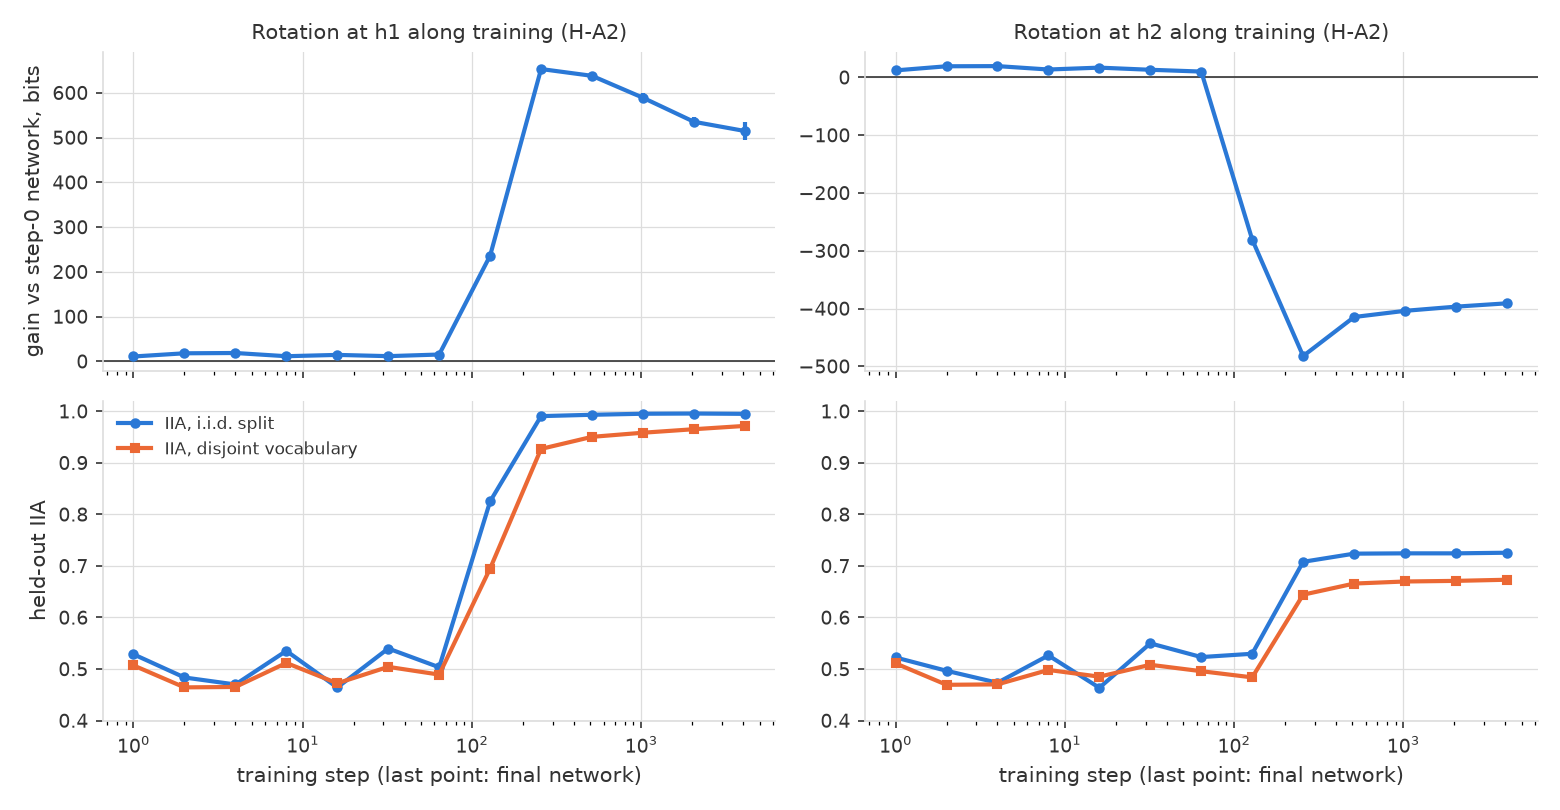
\includegraphics[width=\textwidth]{../stage1_toy/trajectory_dv4_mix4_rr.png}
\caption{Competence onset on hierarchical equality: gain of the rotation at $h_1$ (left) and $h_2$ (right) against the step-0 network along training (top), and held-out IIA on the i.i.d.\ and disjoint-vocabulary splits (bottom).}
\label{fig:trajectory}
\end{figure}

\paragraph{Competence onset in the code.} The competence-onset hypothesis says that the code gain of a valid alignment appears when the network becomes competent at the task. Figure~\ref{fig:trajectory} tests it by scoring the rotation at $h_1$ on each saved training checkpoint. Gains over label-only are within $+1.7$ to $+9.5$ bits for checkpoints 1--64, rise to $+226.9\pm3.2$ at step 128 (IIA 0.8 / 0.7 on the i.i.d.\ / shifted splits) and $+643.9\pm6.6$ at step 256 (IIA 1.0 / 0.9), then settle to $+628.7$, $+579.8$, $+526.1$ at steps 512, 1024, 2048 and $+505.5$ at the final network. Against the step-0 network the gain peaks at about $+650$ bits exactly at competence onset and stays positive ($+515$ at the end). Without the noise channel and with the single-map plug-in learner, the same curve had risen to $+375$ bits and then fallen to $-480$ as training continued (Section~\ref{sec:channel}); with the channel the readout's growing confidence no longer penalises the code. At $h_2$ the gain against step 0 goes from about $+10$ to about $-480$ bits between steps 64 and 256 ($-496.2$ over label-only at step 256 against $-13.9$ for the untrained network) as IIA rises only to 0.72: the code separates a correct from a mis-specified locus at the moment the network becomes competent.

\begin{figure}[htbp]
\centering
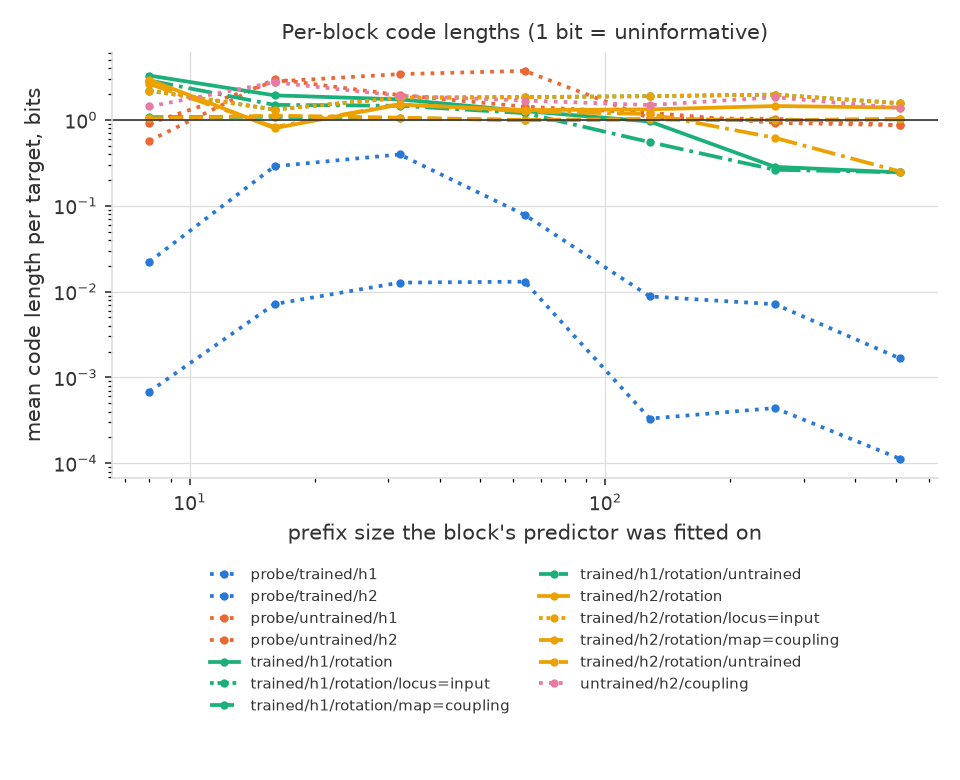
\includegraphics[width=0.8\textwidth]{../stage1_toy/block_losses_dv4_mix4_rr.png}
\caption{Per-block code lengths on hierarchical equality (bits per target as a function of the prefix the block's predictor was fitted on; 1 bit is uninformative for a binary target). The valid rotation at $h_1$ and the coupling maps on the trained network fall to about 0.25 bits per target; every control stays near or above 1 bit.}
\label{fig:toyblocks}
\end{figure}

\subsection{InterpBench case 18}
\label{sec:res:ib18}

\begin{table}[htbp]
\centering\small
\caption{InterpBench case 18, variable \texttt{freq}, three seeds, $\dv=4$ and $\dv=8$. Gains over the label-only code (1341.8 bits); IIA on the held-out i.i.d.\ split (InterpBench has no shifted split); log loss in nats. The wrong locus is \texttt{resid\_0} (attainable IIA 0.46 against 0.84 at \texttt{resid\_1} and 1.00 at \texttt{resid\_2}). The adversary is the coupling map (width 64, 2 blocks, 400 steps) on the untrained twin at \texttt{resid\_2}. The certified distortion bounds of the coupling maps are $10^{6}$--$10^{8}$ (not shown); those of the rotations are 1.}
\label{tab:ib18}
\resizebox{\textwidth}{!}{%
\begin{tabular}{lrrcc}
\toprule
configuration & $\dv=4$ & $\dv=8$ & IIA iid & log loss\\
\midrule
trained / \texttt{resid\_2} / rotation (valid) & $+982.6\pm11.2$ & $+995.9\pm7.7$ & 1.0 & 0.2\\
\quad wrong locus (\texttt{resid\_0}) & $-963.4\pm21.1$ & $-894.3\pm22.3$ & 0.4--0.5 & 1.5--1.6\\
\quad other family (coupling at \texttt{resid\_2}) & $+53.7\pm146.5$ & $+182.7\pm54.8$ & 0.8 & 0.3--0.5\\
\quad untrained twin & $-295.5\pm0.7$ & $-295.5\pm0.7$ & 0.4 & 1.1\\
trained / \texttt{resid\_1} / rotation & $+635.6\pm9.3$ & $+718.9\pm21.8$ & 0.9--1.0 & 0.2--0.3\\
\quad other family (coupling at \texttt{resid\_1}) & $-412.4\pm84.4$ & $-642.0\pm78.1$ & 0.5 & 1.2--1.3\\
\quad untrained twin & $-295.2\pm0.5$ & $-294.3\pm0.3$ & 0.4 & 1.1\\
untrained / \texttt{resid\_2} / coupling (adversary) & $-437.3\pm31.3$ & $-429.5\pm32.9$ & 0.6 & 0.9\\
\quad same on twin seed 8 & $-504.2\pm8.5$ & $-413.9\pm74.3$ & 0.6 & 0.8--0.9\\
\midrule
\multicolumn{5}{l}{\emph{gains against matched controls}}\\
\texttt{resid\_2} rotation vs.\ wrong locus & $+1946.1\pm10.7$ & $+1890.2\pm22.7$\\
\texttt{resid\_2} rotation vs.\ untrained twin & $+1278.1\pm10.5$ & $+1291.3\pm7.0$\\
\texttt{resid\_2} rotation vs.\ coupling & $+928.9\pm148.2$ & $+813.2\pm62.4$\\
\texttt{resid\_1} rotation vs.\ untrained twin & $+930.8\pm9.0$ & $+1013.2\pm21.6$\\
adversary vs.\ twin seed 8 & $+67.0\pm23.6$ & $-15.7\pm42.0$ & \multicolumn{2}{l}{per seed $+20,+92,+89$ / $-22,+60,-85$}\\
\bottomrule
\end{tabular}%
}
\end{table}

Table~\ref{tab:ib18} gives both widths. The valid rotation at \texttt{resid\_2} gains $+982.6\pm11.2$ ($\dv=4$) and $+995.9\pm7.7$ ($\dv=8$) bits over label-only, about $+1280$ over the untrained twin and about $+1900$ over the embedding locus, all decisive; its IIA is 1.0 on the held-out i.i.d.\ split. The two widths differ by $13\pm14$ bits, i.e.\ equivalent representational choices code equally here. The rotation at \texttt{resid\_1} (IIA 0.9 at $\dv=4$) is also strongly positive but codes about 350 bits longer than \texttt{resid\_2} at $\dv=4$. The coupling map on the trained network is only marginally better than label-only and has large seed variance. The adversary (IIA 0.6, so not convincing) codes about 430 bits longer than label-only and, against the same map on twin seed 8, gains $+67.0\pm23.6$ bits ($\dv=4$; below the 100-bit floor) and $-15.7\pm42.0$ ($\dv=8$).

\begin{figure}[htbp]
\centering
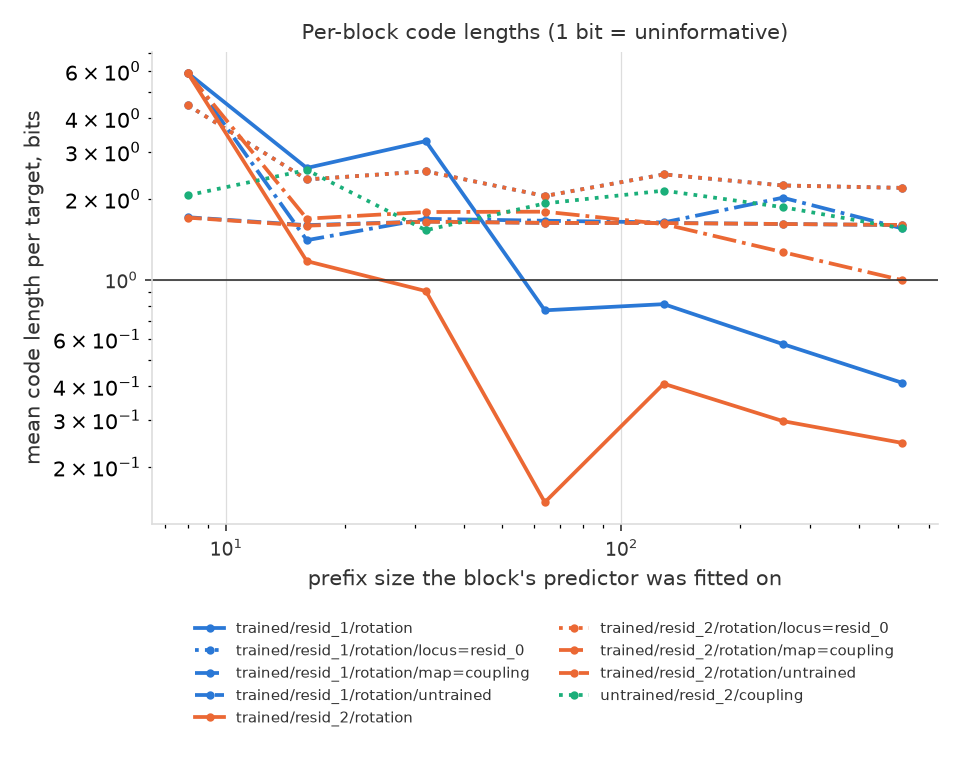
\includegraphics[width=0.8\textwidth]{../stage1_interpbench/case18_block_losses_dv4_mix4_rr.png}
\caption{Per-block code lengths on InterpBench case 18 at $\dv=4$. The valid rotation at \texttt{resid\_2} falls to 0.25--0.4 bits per target from the fourth block on; the rotation at \texttt{resid\_1} follows more slowly; every control stays above 1 bit.}
\label{fig:ibblocks}
\end{figure}

\subsection{InterpBench case 7}
\label{sec:ib7}

\begin{table}[htbp]
\centering\small
\caption{InterpBench case 7, variable \texttt{count}, three seeds, $\dv=4$. Gains over the label-only code (2700.0 bits); IIA on the held-out i.i.d.\ split. The wrong locus is \texttt{resid\_0} (attainable IIA 0.17 against 0.99 at \texttt{resid\_1} and 1.00 at \texttt{resid\_2}; probe accuracy 0.29 against 0.97--0.98). The adversary is the coupling map (width 64, 2 blocks, 400 steps) on the untrained twin at \texttt{resid\_2}; no second twin was scored on this case.}
\label{tab:ib7}
\resizebox{\textwidth}{!}{%
\begin{tabular}{lrccc}
\toprule
configuration & gain over label-only & IIA iid & log loss & dist.\ bound\\
\midrule
trained / \texttt{resid\_2} / rotation & $+2012.0\pm4.0$ & 1.0 & 0.3 & 1\\
\quad wrong locus (\texttt{resid\_0}) & $-2009.1\pm23.1$ & 0.2 & 3.4 & 1\\
\quad other family (coupling at \texttt{resid\_2}) & $+1700.0\pm23.2$ & 1.0 & 0.3 & $2.6\times10^{4}$\\
\quad untrained twin & $-802.3\pm0.7$ & 0.1 & 2.4 & 1\\
trained / \texttt{resid\_1} / rotation & $+1874.7\pm51.5$ & 1.0 & 0.5 & 1\\
\quad other family (coupling at \texttt{resid\_1}) & $-1010.4\pm461.6$ & 0.3 & 2.4 & $7.8\times10^{5}$\\
\quad untrained twin & $-791.9\pm1.3$ & 0.1 & 2.4 & 1\\
untrained / \texttt{resid\_2} / coupling (adversary) & $-865.3\pm67.0$ & 0.6 & 1.2 & $3\times10^{6}$\\
\midrule
\multicolumn{5}{l}{\emph{gains against matched controls}}\\
\texttt{resid\_2} rotation vs.\ wrong locus / untrained twin / coupling & \multicolumn{4}{l}{$+4021.1\pm23.2$ / $+2814.3\pm4.6$ / $+312.0\pm23.1$}\\
\texttt{resid\_1} rotation vs.\ wrong locus / untrained twin / coupling & \multicolumn{4}{l}{$+3883.8\pm74.6$ / $+2666.6\pm50.6$ / $+2885.1\pm466.0$}\\
\bottomrule
\end{tabular}%
}
\end{table}

Cases 7 and 52 were run after the preregistered evaluation had been decided (Section~\ref{sec:gate}), with the canonical learner and the protocol of case~18 (Section~\ref{sec:tb:ib}). Table~\ref{tab:ib7} gives case~7, whose variable \texttt{count} is the output itself. The rotation at \texttt{resid\_2} gains $+2012.0\pm4.0$ bits over label-only, $+2814.3\pm4.6$ over the untrained twin and $+4021.1\pm23.2$ over the embedding locus, all decisive, at IIA 1.0 on the held-out i.i.d.\ split; the rotation at \texttt{resid\_1} is also faithful (IIA 1.0) and codes about 140 bits longer (difference of the two means). Unlike on case~18, the rotation beats the coupling map at its own locus here ($+312.0\pm23.1$). The adversary reaches IIA 0.6 and codes $865.3\pm67.0$ bits longer than label-only: it is rejected under the absolute form of the rejection criterion (Section~\ref{sec:prereg}).

\subsection{InterpBench case 52}
\label{sec:ib52}

\begin{table}[htbp]
\centering\small
\caption{InterpBench case 52, variable \texttt{value}, three seeds, $\dv=4$. Gains over the label-only code (3535.2 bits); IIA on the held-out i.i.d.\ split. The wrong locus is \texttt{resid\_1}, selected by the causal rule; the original decodability rule had selected \texttt{resid\_2}, the locus of the valid hypothesis (see text). The \texttt{resid\_1} hypothesis sits at the selected locus and therefore has no wrong-locus control. The adversary is the coupling map (width 64, 2 blocks, 400 steps) on the untrained twin at \texttt{resid\_2}; no second twin was scored on this case.}
\label{tab:ib52}
\resizebox{\textwidth}{!}{%
\begin{tabular}{lrccc}
\toprule
configuration & gain over label-only & IIA iid & log loss & dist.\ bound\\
\midrule
trained / \texttt{resid\_2} / rotation (valid) & $+1186.8\pm126.4$ & 1.0 & 0.6 & 1\\
\quad wrong locus (\texttt{resid\_1}) & $-1244.1\pm30.7$ & 0.2 & 3.1 & 1\\
\quad other family (coupling at \texttt{resid\_2}) & $+1985.8\pm267.6$ & 0.8 & 0.6 & $3.5\times10^{3}$\\
\quad untrained twin & $+35.0\pm0.1$ & 0.1 & 2.4 & 1\\
trained / \texttt{resid\_1} / rotation (mis-specified) & $-1244.1\pm30.7$ & 0.2 & 3.1 & 1\\
\quad other family (coupling at \texttt{resid\_1}) & $-2682.5\pm48.6$ & 0.1 & 4.3 & $1.1\times10^{5}$\\
\quad untrained twin & $+35.5\pm0.1$ & 0.1 & 2.4 & 1\\
untrained / \texttt{resid\_2} / coupling (adversary) & $-93.1\pm26.4$ & 0.6 & 1.2 & $1.4\times10^{6}$\\
\midrule
\multicolumn{5}{l}{\emph{gains against matched controls}}\\
\texttt{resid\_2} rotation vs.\ wrong locus / untrained twin / coupling & \multicolumn{4}{l}{$+2430.9\pm151.1$ / $+1151.8\pm126.4$ / $-799.0\pm288.0$}\\
\texttt{resid\_1} rotation vs.\ untrained twin / coupling & \multicolumn{4}{l}{$-1279.6\pm30.7$ / $+1438.4\pm76.2$}\\
\bottomrule
\end{tabular}%
}
\end{table}

Table~\ref{tab:ib52} gives case~52, the elementwise square root, whose variable \texttt{value} is the input token at the output position. The rotation at \texttt{resid\_2} is the valid hypothesis (IIA 1.0 on the held-out i.i.d.\ split) and gains $+1186.8\pm126.4$ bits over label-only and $+1151.8\pm126.4$ over the untrained twin, decisive on size and on the all-seeds test, with a larger seed spread than on cases 7 and 18. Against its wrong-locus control at \texttt{resid\_1} it gains $+2430.9\pm151.1$ bits (peak running evidence $2432.3\pm150.7$ bits; every seed rejects the control at $\alpha=0.01$ by $n=345$; Section~\ref{sec:anytime}). The coupling map at the same locus codes $799.0\pm288.0$ bits shorter still ($+1985.8\pm267.6$ over label-only) at IIA 0.8: the other-family comparison again goes against the rotation, as on hierarchical equality. The hypothesis at \texttt{resid\_1} is mis-specified (IIA 0.2) and is correctly rejected: $1279.6\pm30.7$ bits behind the untrained twin and $1244.1\pm30.7$ behind label-only. The adversary (IIA 0.6) codes $93.1\pm26.4$ bits longer than label-only and gains nothing.

\paragraph{Why the wrong-locus rule was changed.} In neither case~7 nor case~52 is the variable computed by the network from other variables: in case~7 it is the output, and in case~52 it is a copy of an input token. We call the latter a \emph{copy variable}. The notion of ``a locus before $V$ is computed'' does not exist for such a variable, and case~52 showed that the original operationalisation by decodability fails on it. Because \texttt{value} is the input token itself, a held-out logistic probe decodes it perfectly from the embedding (accuracy 1.0 at \texttt{resid\_0}) and only slightly less well downstream (0.96 at \texttt{resid\_1}, 0.91 at \texttt{resid\_2}). The least-decodable rule therefore selected \texttt{resid\_2}---the locus of the valid hypothesis---as the ``wrong locus''. Under that rule the wrong-locus control of the \texttt{resid\_2} hypothesis coincided with the hypothesis and was not scored, and the ``wrong locus'' of the \texttt{resid\_1} hypothesis was the valid alignment, which is why the \texttt{resid\_1} rotation then lost $2430.9\pm151.1$ bits to its ``wrong locus'' (the same pair of codes that now appears, with the opposite sign, as the valid hypothesis's gain over its control). The verdicts did not rest on this control (they rest on label-only and the untrained twin), but the control was mis-specified for copy variables. After this failure, and post hoc, the rule was replaced by the causal rule of Section~\ref{sec:setup}: the wrong locus is the locus at which the hypothesis's own map family attains the lowest held-out IIA in two cold-start fits. On case~52 it selects \texttt{resid\_1}: attainable IIA 0.11 against 0.99 at the embedding and 0.64 at \texttt{resid\_2} in the check that fixed the rule, and 0.253 against 0.949 and 0.994 in the re-run that recomputed the case-52 wrong-locus records; both evaluations select \texttt{resid\_1}. On every other testbed the causal rule reproduces the original choice, so only case~52's wrong-locus records changed, and Table~\ref{tab:ib52} reports the recomputed ones. Decodability is still reported as a diagnostic.

\subsection{IOI in GPT-2 small}
\label{sec:res:ioi}

Recall from Section~\ref{sec:tb:ioi} that every GPT-2 prompt has the form ``When X and Y went to the PLACE, S gave a/the OBJECT to'' (the only two of the five templates that survive the equal-token-length filter), that the variable \texttt{io} is the identity of the indirect object and the output alphabet is the 32 single-token names ($K=32$), and that the locus \texttt{layer}$\ell$ is the residual stream entering block~$\ell$ at the final position: layer~0 is the token-plus-position embedding and layer~12 is the state after the final layer normalisation, which only the unembedding follows. The wrong locus is layer~0 (attainable IIA 0.072, 0.069, 0.093, 0.971, 0.997 and 0.973 at layers 0, 6, 9, 10, 11 and 12; loci within 0.02 of the minimum count as tied and the earliest wins).

\begin{table}[htbp]
\centering\small
\caption{IOI in GPT-2 small, variable \texttt{io}, subspace maps with $\dv=16$ at the final position, five seeds. Gains over the label-only code (4324.5 bits). IIA on the i.i.d.\ split and on the disjoint-name split. The main-run adversary is the coupling map (width 512, 4 blocks, 4000 steps) on the untrained twin at layer 6.}
\label{tab:gpt2}
\resizebox{\textwidth}{!}{%
\begin{tabular}{lrcccc}
\toprule
configuration & gain over label-only & IIA iid & IIA shifted & log loss & dist.\ bound\\
\midrule
trained / layer 10 / subspace (valid) & $+2974.6\pm3.0$ & 1.0 & 0.1 & 0.6 & 1\\
trained / layer 11 / subspace (valid) & $+3301.7\pm3.0$ & 1.0 & 0.1 & 0.5 & 1\\
trained / layer 12 / subspace (valid) & $+3145.0\pm2.6$ & 1.0 & 0.1 & 0.5 & 1\\
trained / layer 9 / subspace & $-2481.6\pm1.7$ & 0.1 & 0.1 & 4.5 & 1\\
trained / layer 6 / subspace & $-2492.1\pm12.1$ & 0.1 & 0.0 & 4.5 & 1\\
wrong locus: trained / layer 0 / subspace & $-3517.9\pm0.0$ & 0.1 & 0.1 & 5.4 & 1\\
untrained twin at layer 10 / 11 / 12 & $+22.4\pm1.4$ / $+45.5\pm1.4$ / $+63.2\pm1.8$ & 0.2 & 0.0 & 2.8--2.9 & 1\\
coupling on trained net at layer 10 & $+2902.7\pm17.2$ & 1.0 & 0.1 & 0.4 & $2.3\times10^{6}$\\
coupling on trained net at layer 11 & $+2896.0\pm9.3$ & 1.0 & 0.1 & 0.5 & $2.6\times10^{6}$\\
coupling on trained net at layer 12 & $+1812.7\pm19.2$ & 0.9 & 0.0 & 0.6 & $1.6\times10^{5}$\\
untrained / layer 6 / coupling (adversary) & $+60.5\pm137.9$ & 0.9 & 0.0 & $1.0\pm0.1$ & $1\times10^{16}$\\
\midrule
\multicolumn{6}{l}{\emph{gains against matched controls}}\\
layer 10 vs.\ layer 0 / untrained / coupling & \multicolumn{5}{l}{$+6492.5\pm3.0$ / $+2952.1\pm2.8$ / $+71.9\pm17.2$}\\
layer 11 vs.\ layer 0 / untrained / coupling & \multicolumn{5}{l}{$+6819.6\pm3.0$ / $+3256.2\pm2.6$ / $+405.7\pm10.0$}\\
layer 12 vs.\ layer 0 / untrained / coupling & \multicolumn{5}{l}{$+6662.9\pm2.6$ / $+3081.9\pm3.6$ / $+1332.4\pm20.2$}\\
\bottomrule
\end{tabular}%
}
\end{table}

Table~\ref{tab:gpt2} gives the main GPT-2 run. The three valid loci gain $+2974.6$, $+3301.7$ and $+3145.0$ bits over label-only, about $+3000$ over their untrained twins and $+6500$--$6800$ over the embedding locus, with standard errors of about 3 bits over five seeds and every seed positive. (The preregistered evaluation was decided on the first three seeds of the same run, whose layer-11 values are $+3299\pm3$ / $+3253\pm3$ / $+6816\pm3$ over label-only, the untrained twin and layer~0; the two further seeds changed the gains by at most 3 bits.) Their i.i.d.\ IIA is 1.0; their disjoint-name IIA is 0.1, i.e.\ no subspace map transfers to unseen names (Section~\ref{sec:limits}). Layers 6 and 9 behave like the wrong locus (IIA 0.1, held-out log loss about 4.5 nats per target), consistent with the learner-specification sweep (Section~\ref{sec:tb:ioi}). The coupling map on the trained network is close to the subspace map at layers 10 and 11 and well behind it at layer 12.

The three valid loci do not code equally: layer~11 codes $327\pm3$ bits shorter than layer~10 and $157\pm4$ bits shorter than layer~12 over five seeds. The shorter code belongs to the more faithful map (IIA 0.99 against 0.97, log loss 0.50 against 0.62 nats for layer~11 against layer~10). By code length the loci are ordered $11 < 12 < 10$.

\paragraph{No subspace illusion.}\label{sec:res:illusion} An interchange on a learned subspace can succeed through an illusion \cite{makelov2024}: a part that varies with the variable but is disconnected from the output, together with a dormant part that is connected, so that neither part works alone. The learned subspaces were checked for this on GPT-2 (layers 10--12), Pythia-1.4b (final checkpoint, layers 16, 18 and 20) and Qwen2.5-0.5B (layers 22 and 24), with one cold-start single-map fit of the $\dv=16$ subspace on the same 1024 targets for each of three seeds. The per-prompt Jacobians of the log-softmax over the 32 names with respect to the locus define the output-connected subspace $C$ that holds 99\% of their energy. The fitted subspace $U$ is split into its connected and disconnected parts, each part is patched alone, and its IIA is measured on the 1000 i.i.d.\ pairs; the directions of $U$ are profiled by their sensitivity, by their variance across prompts (dormancy) and by the share of that variance explained by the IO name. There is no illusion at any locus of the three models. The disconnected part alone is at the no-effect level 0.072 (the share of pairs whose counterfactual equals the base's own answer) everywhere, and the connected part alone reproduces the full IIA (0.93--1.00), except at Pythia layer~16 (0.80 against 0.93). The most sensitive direction of $U$ varies 6--43 times more across prompts than a random direction, and the IO name explains 82--91\% of its variance (random directions: 23--54\%). Between 21\% and 52\% of each $U$ lies outside $C$ and does nothing when patched, about half at the final loci (GPT-2 layer~12, Qwen2.5-0.5B layer~24). At a residual-stream locus every later layer reads the state, so the split is by local sensitivity at the base states, not by the row space of one linear map as in Makelov et al.; the check covers the learned subspaces on IOI only, not the coupling maps or the other testbeds.

\begin{figure}[htbp]
\centering
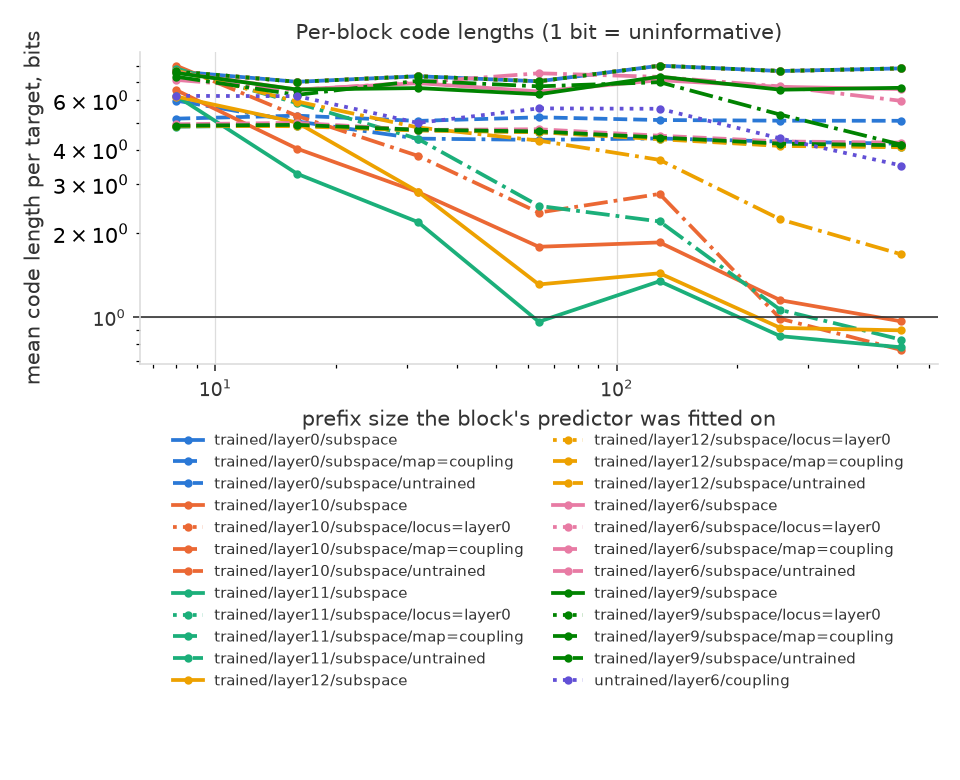
\includegraphics[width=0.8\textwidth]{../stage1_ioi/gpt2_block_losses_v2.png}
\caption{Per-block code lengths on IOI in GPT-2 small (1 bit per target is far from uninformative here: the uniform code over 32 names is 5 bits). The subspace maps at layers 10--12 fall below 1 bit per target from the sixth block on; the layer-6 adversary (dotted, purple) descends slowly from about 6 to 3.5 bits.}
\label{fig:gpt2blocks}
\end{figure}

\begin{figure}[htbp]
\centering
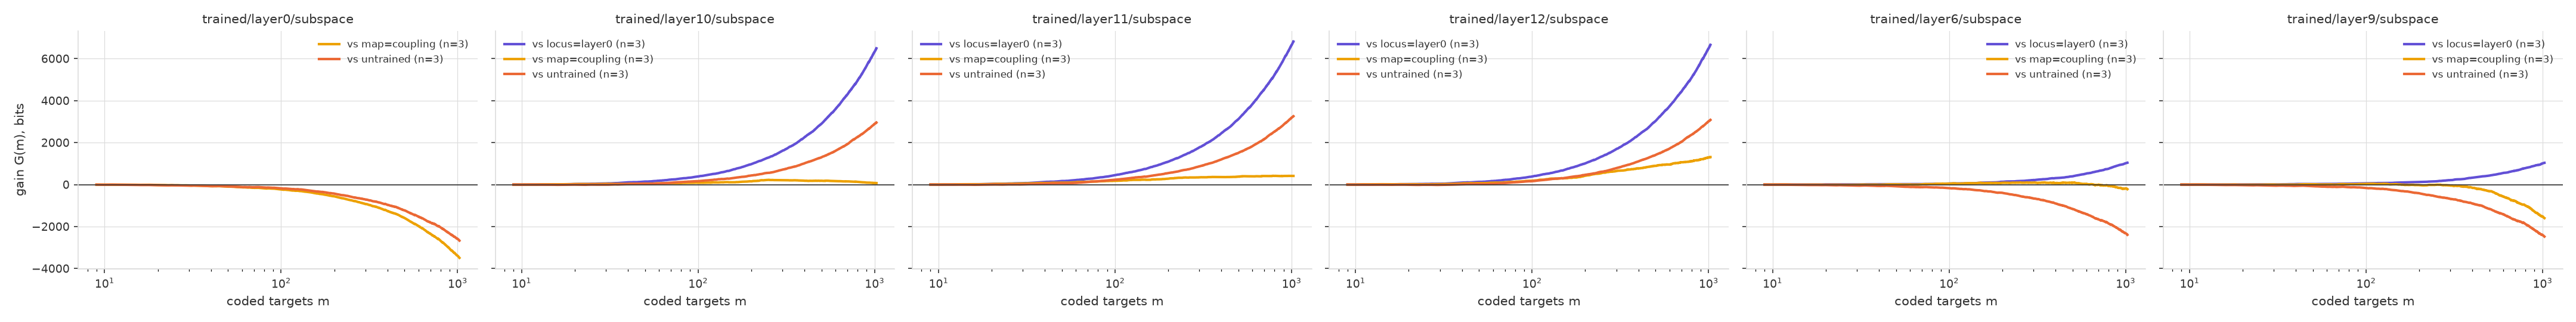
\includegraphics[width=\textwidth]{../stage1_ioi/gpt2_gain_curves_v2.png}
\caption{Cumulative gain $G(m)$ of each GPT-2 subspace hypothesis against its three controls as a function of the number of coded targets $m$ (three-seed version of the run). At layers 10--12 the gains against the wrong locus and the untrained twin grow without bound; at layers 0, 6 and 9 they are flat or negative.}
\label{fig:gpt2gains}
\end{figure}

\subsection{IOI in larger language models}
\label{sec:res:ioilm}

The GPT-2 protocol was run on Llama-3.1-8B, Qwen2.5-3B and Qwen3-1.7B without tuning (Section~\ref{sec:tb:ioilm}). The targets are those of GPT-2, so the label-only code is 4324.5 bits throughout. Llama-3.1-8B and Qwen2.5-3B have one seed under the single-map MAP learner; Qwen3-1.7B has three seeds under the mixture of four. Table~\ref{tab:ioilm} gives the gains over label-only with the i.i.d.\ IIA.

\begin{table}[htbp]
\centering\small
\caption{IOI in three larger language models, variable \texttt{io}, $\dv=16$, the targets of Table~\ref{tab:gpt2}. Gains over the label-only code (4324.5 bits), i.i.d.\ IIA in brackets. ``Twin'' is the same subspace family on the untrained twin, ``coupling'' the coupling family on the trained network, both at the same locus. The manufactured alignment is the coupling map with 4000 steps on the twin at the strongest valid locus. Lower block: gains of the valid subspace at the strongest locus against its controls, with the coded index by which the running evidence first exceeds $\log100$ ($\alpha=0.01$). For reference, GPT-2 layer~11 gains $+3384.6\pm4.9$ under the MAP learner and $+3301.7\pm3.0$ under the mixture.}
\label{tab:ioilm}
\resizebox{\textwidth}{!}{%
\begin{tabular}{lllll}
\toprule
model (learner, seeds) & locus & subspace & twin & coupling\\
\midrule
Llama-3.1-8B (MAP, 1) & layer 28 & $+3018$ (0.93) & $-537$ (0.27) & $+1635$ (0.89)\\
 & layer 30 & $+3101$ (0.92) & $-639$ (0.27) & $+1436$ (0.87)\\
 & layer 32 & $+1709$ (0.71) & $-606$ (0.33) & $+827$ (0.93)\\
 & layer 0 (wrong locus) & $-3527$ (0.07) & & \\
 & manufactured, layer 30 & \multicolumn{3}{l}{$-1830$ (0.51)}\\
\midrule
Qwen2.5-3B (MAP, 1) & layer 32 & $-445$ (0.24) & $+183$ (0.41) & $-667$ (0.67)\\
 & layer 34 & $+3129$ (0.94) & $+223$ (0.43) & $+1690$ (0.89)\\
 & layer 36 & $+2702$ (0.90) & $+188$ (0.42) & $+1385$ (0.90)\\
 & layer 0 (wrong locus) & $-3548$ (0.07) & & \\
 & manufactured, layer 34 & \multicolumn{3}{l}{$-1723$ (0.59)}\\
\midrule
Qwen3-1.7B-Base (mixture, 3) & layer 22 & $+712\pm2$ (0.40) & $+618\pm4$ (0.54) & $+1548\pm47$ (0.90)\\
 & layer 26 & $+3001\pm4$ (0.97) & $+660\pm3$ (0.56) & $+2318\pm61$ (0.97)\\
 & layer 28 & $+3042\pm3$ (0.99) & $+692\pm1$ (0.57) & $+2047\pm25$ (0.96)\\
 & layer 0 (wrong locus) & $-3137$ (0.07) & & \\
 & manufactured, layer 26 & \multicolumn{3}{l}{pending (jobs 1814205--1814207)}\\
\midrule
\multicolumn{5}{l}{\emph{valid subspace against its controls: twin / coupling / layer 0 (rejects at $\alpha=0.01$ by $n$)}}\\
Llama-3.1-8B, layer 30 & \multicolumn{4}{l}{$+3740$ (12) / $+1665$ (9) / $+6628$ (9)}\\
Qwen2.5-3B, layer 34 & \multicolumn{4}{l}{$+2906$ (20) / $+1439$ (11) / $+6678$ (13)}\\
Qwen2.5-3B, layer 32 & \multicolumn{4}{l}{$-628$ (never) / $+222$ (19) / $+3104$ (13)}\\
\bottomrule
\end{tabular}}
\end{table}

\paragraph{The verdicts transfer.} At the loci where the name is intervenable the valid subspace gains 3000--3130 bits over label-only on every model: $+3101$ on Llama-3.1-8B at layer~30 and $+3129$ on Qwen2.5-3B at layer~34 under the MAP learner, against $+3385$ for GPT-2 under the same learner, and $+3042\pm3$ on Qwen3-1.7B at layer~28 under the mixture, against $+3302$ for GPT-2. The single-seed gains clear the 216-bit size floor of the decisive-gain rule more than sixfold against every control; its significance clause needs several seeds and is not defined for one, and the anytime evidence carries the statistical statement instead: the valid alignment rejects the untrained twin, the other family and the wrong locus at $\alpha=0.01$ within the first 9--20 coded targets on both single-seed models. The manufactured alignment never beats label-only ($-1830$ and $-1723$ bits) although its IIA, 0.51 and 0.59, would pass an accuracy threshold of one half (Section~\ref{sec:adversary}). The intervenable loci are the last two to four layers of every model: layers 28--30 of 32 on Llama-3.1-8B, 34 of 36 on Qwen2.5-3B, 26--28 of 28 on Qwen3-1.7B.

\paragraph{The code charges the other family; IIA does not.} At the intervenable loci of Llama-3.1-8B and Qwen2.5-3B the coupling family on the trained network is 1300--1700 bits behind the subspace at the same locus, at an IIA at most 0.05 below the subspace's: on Llama-3.1-8B at layer~30 by 1665 bits (IIA 0.87 against 0.92), on Qwen2.5-3B at layer~34 by 1439 bits (0.89 against 0.94) and at layer~36 by 1317 bits at equal IIA (0.90). On Qwen3-1.7B under the mixture the gap is smaller, about 680 bits at layer~26 at equal IIA (0.97). At Llama's layer~32 the coupling map is the more faithful of the two (IIA 0.93 against 0.71) and still codes 882 bits longer. The plug-in code pays for the family's Fisher-weighted complexity (Section~\ref{sec:coef}), which IIA does not see.

\paragraph{A locus that is decodable but not intervenable.} Layer~32 of Qwen2.5-3B is read by a held-out probe with accuracy 0.90, but the attainable IIA of the subspace map there is 0.24. The code agrees with the interventions, not with the probe: the valid family codes 445 bits longer than label-only and loses 628 bits to its own untrained twin ($+183$), whose running evidence it never overcomes. This is the first locus in this paper at which the untrained twin beats the trained network. The coupling map reaches IIA 0.67 there and codes 667 bits longer than label-only.

\paragraph{The controls differ between models; the valid gain does not.} The untrained twin is weak on Llama-3.1-8B ($-537$ to $-639$ bits, IIA 0.27--0.33), close to label-only on Qwen2.5-3B ($+183$ to $+223$, IIA 0.41--0.43) and strong on Qwen3-1.7B ($+618$ to $+692$, IIA 0.54--0.57): the untrained Qwen3 residual stream carries the name tokens almost linearly, as Pythia's does (IIA 0.39, Section~\ref{sec:res:pythia}), and the valid alignment still beats it by about 2300 bits. The valid gain is nearly model-independent because it is dominated by $n$ times the loss gain of a near-perfect predictor on 1016 targets behind the 5\% channel; the models differ in the strength of the controls and in where the intervenable loci sit.

\paragraph{Gemma-2-2b.} The locus sweep on Gemma-2-2b gives subspace IIA on the i.i.d.\ split of 0.08--0.10 at layers 0--16, 0.52 and 0.58 ($\dv=16$ and 64) at layer~20, 0.64 and 0.70 at layer~22, 0.99 at layer~24, and 0.96 and 0.99 at layer~26. The coupling map does not learn at learning rate $10^{-2}$ on this model (loss 3.47 nats, IIA 0.08 at every layer), so a run of the score on Gemma IOI needs the coupling learning rate $10^{-3}$ used for the adversary, at loci 22, 24 and 26. It has not been run.

\subsection{Competence onset in Pythia-1.4b}
\label{sec:res:pythia}

The competence-onset hypothesis (Section~\ref{sec:tb:heq}) was tested on hierarchical equality along the training checkpoints of the MLP (Figure~\ref{fig:trajectory}). Pythia-1.4b gives the same test on a pretrained language model. Its IOI competence on our prompts appears between steps 1000 and 4000, i.e.\ between about 2 and 8 billion training tokens (Table~\ref{tab:pythia}): the share of prompts on which the IO outscores the subject among the 16 training names is 0.09 at step 1000 (chance is $1/16$), 0.43 at 2000, 0.95 at 4000 and 1.00 from step 8000 on, and the IO is the most probable token of the whole vocabulary on 0.00, 0.13, 0.68 and 0.99 of the prompts at the same steps. The score was run at seven checkpoints with the single-map MAP learner and one seed (Section~\ref{sec:tb:ioilm}); checkpoints 32000 and 64000 were not run. The untrained twin is a fresh initialisation under seed 7 and is therefore the same at every checkpoint, as is the manufactured alignment on it (the coupling map with 400 steps at layer~20).

\begin{table}[htbp]
\centering\small
\caption{Pythia-1.4b along training, IOI, single-map MAP code, one seed. Code lengths in bits on the 1016 coded targets (label-only 4324.5 bits), i.i.d.\ IIA in brackets. ``Accuracy'' is the share of 400 prompts on which the IO outscores the subject among the 16 training names (not measured at step 3000). Twin: the subspace map on the untrained twin at layer 20. Coupling: the coupling map on the trained checkpoint at layer 20. Manufactured: the 400-step coupling map on the twin at layer 20.}
\label{tab:pythia}
\begin{tabular}{rclllll}
\toprule
step & accuracy & valid, layer 16 & valid, layer 20 & twin & coupling & manufactured\\
\midrule
1000 & 0.09 & 4800 (0.15) & 4748 (0.15) & 3751 (0.39) & 5524 (0.61) & 4968 (0.78)\\
2000 & 0.43 & 2857 (0.57) & 2833 (0.58) & 3751 (0.39) & 4306 (0.75) & 4968 (0.78)\\
3000 & -- & 1544 (0.94) & 1451 (0.93) & 3751 (0.39) & 2778 (0.92) & 4968 (0.78)\\
4000 & 0.95 & 1755 (0.93) & 1551 (0.91) & 3751 (0.39) & 2873 (0.87) & 4968 (0.78)\\
8000 & 1.00 & 1023 (0.99) & 896 (1.00) & 3751 (0.39) & 1953 (0.97) & 4968 (0.78)\\
16000 & 1.00 & 1032 (0.99) & 853 (1.00) & 3751 (0.39) & 1796 (0.95) & 4968 (0.78)\\
143000 & 1.00 & 1545 (0.94) & 910 (0.99) & 3751 (0.39) & 2226 (0.95) & 4968 (0.78)\\
\bottomrule
\end{tabular}
\end{table}

\paragraph{The code tracks competence.} The valid alignment's code is 4750--4800 bits at step 1000, longer than the label-only code, with IIA 0.15; 2830--2860 bits at step 2000 (accuracy 0.43, IIA 0.57); 1450--1540 at step 3000 (IIA 0.93); 1550--1750 at step 4000 (accuracy 0.95); and 850--1030 from step 8000 on (accuracy 1.00, IIA 0.99--1.00). The name subspace becomes compressible when the task is solved, not before.

\paragraph{The code keeps shortening after the task is solved.} Between steps 4000 and 8000 the accuracy is already 0.95--1.00 and the IIA 0.91--0.93, yet the layer-20 code falls from 1551 to 896 bits: the name subspace goes on becoming cleaner after the task is solved, and the code registers it where accuracy has saturated. (At one seed the code also rises slightly between steps 3000 and 4000, from 1451 to 1551 bits.) On hierarchical equality the gain instead peaked at competence onset and settled afterwards (Section~\ref{sec:res:heq}).

\paragraph{The representation moves to later layers late in training.} At the final checkpoint the layer-20 code is unchanged (910 bits, IIA 0.99), while the layer-16 code is 50\% longer than at step 16000 (1545 against 1032 bits, IIA 0.94).

\paragraph{Controls along training.} The untrained twin's subspace codes the targets in 3751 bits (IIA 0.39): the untrained residual stream still carries the name tokens. It beats the trained network at step 1000, which by then has disrupted the raw copy without yet computing the task. The manufactured alignment on the twin reaches IIA 0.78 with 400 steps, close to the existence threshold of the preregistered evaluation, while its code is 640 bits longer than label-only. The coupling family on the trained network follows the subspace from step 3000 on, about 900--1300 bits behind it at the same locus.

\subsection{Two-digit addition in Llama-3.1-8B and Gemma-2-2b}
\label{sec:res:mib}

Table~\ref{tab:mib} gives the carry variable of MIB's two-digit addition (Section~\ref{sec:tb:mib}) on both models: one seed, the single-map MAP learner, gains over the label-only code with the i.i.d.\ IIA. The row of layer~0 is the trivial floor, the model's own answer, which is also the wrong-locus control; the reference for every alignment is this row, not zero.

\begin{table}[htbp]
\centering\small
\caption{MIB two-digit addition, variable \texttt{carry}, $\dv=16$, single-map MAP code, one seed. Gains over the label-only code (7602.7 bits for Llama-3.1-8B, 199 output symbols; 2280.9 bits for Gemma-2-2b, 10 symbols), i.i.d.\ IIA in brackets. Layer~0 is the trivial floor. The ``vs.'' rows give gains of the subspace map against the floor (layer~0) and against its other controls, with the coded index by which the running evidence first exceeds $\log100$ ($\alpha=0.01$) in brackets.}
\label{tab:mib}
\begin{tabular}{llll}
\toprule
locus & subspace & coupling, trained & untrained twin\\
\midrule
\multicolumn{4}{l}{\emph{Llama-3.1-8B} (label-only 7602.7 bits)}\\
layer 0 (floor) & $+2715$ (0.48) & $+2863$ (0.01) & $-1038$ (0.00)\\
layer 8 & $+2787$ (0.48) & $+2818$ (0.00) & $-904$ (0.00)\\
layer 16 & $+3375$ (0.47) & $+4429$ (0.69) & $-929$ (0.00)\\
layer 20 & $+3768$ (0.49) & $+1876$ (0.96) & $-997$ (0.00)\\
layer 24 & $+3764$ (0.51) & $+5063$ (0.94) & $-1035$ (0.00)\\
layer 28 & $+3528$ (0.49) & $+4085$ (0.86) & $-1056$ (0.00)\\
layer 32 & $+3156$ (0.44) & $+415$ (0.43) & $-1083$ (0.00)\\
manufactured, layer 24 & \multicolumn{3}{l}{$-2160$ (0.14)}\\
subspace vs.\ floor & \multicolumn{3}{l}{layer 16 $+660$ (66), 20 $+1053$ (41), 24 $+1049$ (112), 28 $+813$ (145)}\\
coupling, layer 24 & \multicolumn{3}{l}{$+2348$ against the floor, $+1299$ against the subspace}\\
\midrule
\multicolumn{4}{l}{\emph{Gemma-2-2b} (label-only 2280.9 bits)}\\
layer 0 (floor) & $+719$ (0.78) & $+686$ (0.78) & $-1354$ (0.09)\\
layer 8 & $+744$ (0.78) & $+800$ (0.88) & $-439$ (0.52)\\
layer 12 & $+770$ (0.78) & $+919$ (0.89) & $-542$ (0.50)\\
layer 16 & $+888$ (0.79) & $+814$ (0.86) & $-765$ (0.44)\\
layer 20 & $+1473$ (0.96) & $+1218$ (0.97) & $-878$ (0.42)\\
layer 24 & $+1116$ (0.84) & $+1054$ (0.95) & $-1082$ (0.35)\\
layer 26 & $+528$ (0.78) & $+643$ (0.92) & $-1320$ (0.33)\\
manufactured, layer 20 & \multicolumn{3}{l}{$-1075$ (0.62)}\\
layer-20 subspace vs.\ & \multicolumn{3}{l}{floor $+754$ (16), coupling $+255$ (18), twin $+2351$ (11)}\\
subspace vs.\ floor & \multicolumn{3}{l}{layer 8 $+25$, 12 $+52$, 16 $+169$, 24 $+397$, 26 $-191$}\\
\bottomrule
\end{tabular}
\end{table}

\paragraph{Gemma reads the carry linearly at one locus.} On Gemma-2-2b the subspace map at layer~20 of 26 lifts the IIA from the floor's 0.78 to 0.96 and codes 754 bits shorter than the floor; the loci before and after it fall back to the floor (IIA 0.78--0.84) and gain 25 to 397 bits on it, or lose 191 at layer~26. The layer-20 subspace rejects the floor, the coupling map and the untrained twin by $n=18$. The coupling family on the trained network reaches the same IIA at layer~20 (0.97) and codes 255 bits longer. The code locates the variable by a margin the controls cannot match.

\paragraph{Llama reads it only through the non-linear family.} On Llama-3.1-8B the 16-dimensional subspace never leaves the floor: its IIA is 0.44--0.51 at every layer, although a probe decodes the carry perfectly from layer~20 on, as in the MIB benchmark, where linear methods score near chance on this task and model. The 660--1050 bits it gains over the floor at layers 16--28 come from a better-calibrated predictor (held-out log loss 2.4--2.7 nats against 3.5 at the floor), not from reading the carry, and the running evidence needs 41--145 targets to reject the floor. The coupling family on the trained network does read it: IIA 0.94--0.96 at layers 20--24 and, at layer~24, the shortest code of the run, $+5063$ bits, 2348 bits ahead of the floor and 1299 ahead of the subspace. Its code at layer~20 is about 3200 bits worse than at layer~24 although the IIA is the same: the non-linear learner needs most of the 1024 targets to find the map at layer~20, and the prequential code charges for that. On the untrained twin the same family reaches IIA 0.14 and codes 2160 bits longer than label-only, so the layer-24 alignment is not an artefact of the family's expressiveness. At layers 0 and 8 the coupling map codes near the floor with IIA 0.00--0.01; code and IIA disagree there, and we do not interpret these two rows further.

\paragraph{The code ranks the families in opposite orders on the two models.} The subspace wins on Gemma-2-2b and the coupling map on Llama-3.1-8B, and in each case the winner is the family that is faithful at that locus. A single family, or a single IIA threshold, would have missed one of the two. The manufactured alignments reach IIA 0.14 (Llama-3.1-8B) and 0.62 (Gemma-2-2b, below its 0.78 floor) and never beat the label-only code.

\section{Manufactured alignments}
\label{sec:adversary}

The manufactured alignment of Section~\ref{sec:setup} is the construction of Sutter et al.~\cite{sutter2025}: an expressive invertible map (here the additive coupling map) trained with a large budget to realise the counterfactuals on the \emph{untrained} twin, where no valid alignment can exist. Its IIA is what an alignment search judged by accuracy alone would accept. This section reports how the code treats it.

\paragraph{The main-run adversary (layer 6).} The coupling map on the untrained GPT-2 twin at layer~6 reaches IIA 0.86 on the i.i.d.\ split on every seed and 0.00 on the disjoint-name split, so the accuracy baseline accepts it and a distribution-shift test rejects it. Its code is $60.5\pm137.9$ bits \emph{shorter} than label-only over five seeds (three-seed value $+22\pm98$, per seed $-83,+218,-69$): not decisive on any count, and $3241\pm139$ bits behind the valid hypothesis at layer~11 ($2914\pm139$ at layer~10, $3085\pm137$ at layer~12; paired over five seeds, computed from the per-seed records). With four times the budget (16000 steps, two seeds) it overfits the early blocks and codes $743.6\pm95.0$ bits longer than label-only.

\begin{table}[htbp]
\centering\small
\caption{Adversary sweep on GPT-2: the coupling map (width 512, 4 blocks) on the untrained twin (seed 7) and on a second untrained twin (seed 8), three seeds, gains over the label-only code (4324.5 bits). The unrounded i.i.d.\ IIA of the seed-7 adversary is 0.86 at layer 10 and 0.87 at layer 9. Second twins for layers 6, 11 and 12 were not run.}
\label{tab:adv}
\begin{tabular}{llrccc}
\toprule
locus & steps / twin & gain over label-only & IIA iid & IIA shifted & dist.\ bound\\
\midrule
layer 9 & 4000 / seed 7 & $+290.2\pm43.2$ & 0.9 & 0.0 & $7.2\times10^{11}$\\
layer 9 & 4000 / seed 8 & $+279.8\pm110.1$ & 0.8 & 0.0 & $1\times10^{11}$\\
layer 10 & 4000 / seed 7 & $+704.2\pm62.6$ & 0.9 & 0.0 & $4.1\times10^{16}$\\
layer 10 & 4000 / seed 8 & $+355.0\pm142.1$ & 0.8 & 0.0 & $3.2\times10^{10}$\\
layer 11 & 4000 / seed 7 & $+234.0\pm161.5$ & 0.9 & 0.0 & $1.8\times10^{11}$\\
layer 12 & 4000 / seed 7 & $-1007.6\pm337.7$ & 0.8 & 0.0 & $1\times10^{9}$\\
layer 6 & 16000 / seed 7 (2 seeds) & $-743.6\pm95.0$ & $0.8\pm0.1$ & 0.0 & $1.3\times10^{20}$\\
\midrule
\multicolumn{6}{l}{\emph{comparative form: seed-7 adversary against the seed-8 adversary}}\\
layer 9 & & $+10.5\pm82.3$ & \multicolumn{3}{l}{per seed $-62,+175,-82$}\\
layer 10 & & $+349.1\pm194.8$ & \multicolumn{3}{l}{per seed $+702,+30,+316$}\\
\bottomrule
\end{tabular}
\end{table}

\paragraph{The layer-10 adversary beats label-only.} Table~\ref{tab:adv} gives the sweep over loci. At layer~10 the same map on the untrained twin gains $+704.2\pm62.6$ bits over label-only on every seed, and at layer~9 $+290.2\pm43.2$: both clear the 216-bit floor, the 3-s.e.\ test and the all-seeds test, so under the preregistered rule as first drafted they are \emph{decisive} gains of a manufactured alignment over the reference code. The interpretation is that the untrained residual stream still carries the name tokens through the embedding and the residual connections, and a $1.9$~M-parameter invertible map can decode them within the 16 training names (IIA 0.86 i.i.d., 0.00 on new names). One diagnostic separates it from the valid alignment: the certified distortion bound is $4\times10^{16}$ against 1 for the subspace map. The distribution-shift test does not: the adversary's disjoint-name IIA is 0.00, but the valid subspace map's is 0.1, also at chance (Section~\ref{sec:limits}). The comparative verdicts stand: the valid alignment at layer~10 is ahead of this adversary by $2270\pm62$ bits (paired over the three common seeds: 2188, 2391, 2233; computed from the per-seed records), and the same coupling family on the \emph{trained} network at layer~10 gains $+2902.7\pm17.2$.

\paragraph{First reading and its revision.} The first reading of this result, recorded with the outcome of the preregistered evaluation (Section~\ref{sec:gate}), was that a plug-in code with a fixed training budget does not charge for the complexity of the map: the map's parameters are refitted from scratch at every block and only the labels are paid for, whereas a Bayes or Laplace code over the map family would pay for the parameters through the learning coefficient and the prior. Later runs revised this reading. Scored under single-map learners (one plug-in member, the MAP, or the MAP with a Langevin hedge), the same adversary codes about 1000--2000 bits \emph{longer} than label-only, and the Langevin hedge, the only ingredient that could charge for the parameters, moves the code by about 40 bits: the absolute verdict is decided by the number of maps averaged by the learner, not by a complexity charge (Section~\ref{sec:learner}, Table~\ref{tab:bylearner}). A converged Bayes code, moreover, charges the valid alignment as well, and by more than the label-only code saves (Section~\ref{sec:coef}).

\paragraph{The second-twin control.} The comparative form of the rejection criterion, adopted post hoc (Section~\ref{sec:gate}), scores the adversary against the same map, locus, learner and budget on a second random initialisation (twin seed 8). On hierarchical equality this gain is $-19.1\pm35.6$ bits (five seeds), on InterpBench case~18 $+67.0\pm23.6$ ($\dv=4$) and $-15.7\pm42.0$ ($\dv=8$), on GPT-2 at layer~9 $+10.5\pm82.3$ and at layer~10 $+349.1\pm194.8$ bits with per-seed values $+702$, $+30$, $+316$. The layer-10 case is narrow: it clears the 216-bit floor and every seed is positive, and fails only the 3-s.e.\ test ($349.1/194.8\approx1.8$ s.e.). Two random initialisations of GPT-2 can differ by several hundred bits under an expressive map; that is the noise floor of this control and is reported with the result. The anytime view of the same comparison (Section~\ref{sec:anytime}) shows the same weakness on the small testbeds: the running evidence of the adversary against its second twin crosses the 6.6-bit threshold late or not at all, or crosses early and does not persist.

\paragraph{A stronger manufactured alignment on the small testbeds.} The adversary of the main runs on hierarchical equality and on InterpBench is a coupling map of width 64 with 2 blocks and 400 steps, far below the GPT-2 adversary's $1.9$~M parameters and 4000 steps, so its failure to convince (IIA 0.5 and 0.6) could have been a matter of budget. On hierarchical equality the coupling map with width 256, 4 blocks and 4000 steps on the untrained network at $h_2$ (five seeds; the step-0 twin and twin seed 8) still reaches only IIA 0.5 on both splits, codes $607.6\pm47.2$ bits \emph{longer} than label-only (on twin 8: $453.9\pm58.6$ longer) and $153.7\pm71.1$ bits longer than the same map on its second twin, with a certified distortion bound of $4.5\times10^{14}$. The per-seed codes are $1457$--$1736$ bits on the step-0 twin and $1256$--$1584$ on twin 8 against the label-only $1021$ (gains $-436$ to $-715$ and $-235$ to $-563$; the seed means are the $-607.6\pm47.2$ and $-453.9\pm58.6$ above), at IIA $0.49$--$0.53$ on every seed and twin. The hidden layer of the untrained MLP does not carry the inputs in a form a map of this size decodes within the budget: hierarchical equality admits no convincing false explanation. The same strong adversary on InterpBench case~18 (width 256, 4 blocks, 4000 steps, three seeds, twins 7 and 8) is not convincing either: ten times the training budget leaves its IIA at $0.45$--$0.50$ (chance for the three-valued output is $0.33$; the 400-step version had $0.6$), and its code is $1476$, $1546$ and $2665$ bits on twin 7 and $1566$, $1720$ and $1623$ bits on twin 8 against the label-only $1342$, i.e.\ $134$--$1323$ bits \emph{longer} than label-only on every seed and both twins. The existence criterion (a convincing false explanation exists) therefore stays unmet on both small testbeds, it rests on GPT-2 alone, and the rejection criterion holds on the small testbeds trivially.

\paragraph{Manufactured alignments on the larger models.} The 4000-step coupling map on the untrained twin at the strongest valid locus reaches IIA 0.51 on Llama-3.1-8B (layer~30) and 0.59 on Qwen2.5-3B (layer~34) and codes 1830 and 1723 bits longer than label-only (Table~\ref{tab:ioilm}); the Qwen3-1.7B arm is still running (jobs 1814205--1814207). On Pythia-1.4b the 400-step version reaches IIA 0.78 and codes 640 bits longer than label-only at every checkpoint (Table~\ref{tab:pythia}). On two-digit addition the same 4000-step map reaches IIA 0.14 on Llama-3.1-8B (layer~24) and 0.62 on Gemma-2-2b (layer~20, below the 0.78 floor) and codes 2160 and 1075 bits longer than label-only (Table~\ref{tab:mib}). All of these runs use the single-map MAP learner, under which the GPT-2 layer-10 adversary also codes longer than label-only (Table~\ref{tab:bylearner}). None of them reaches the threshold IIA of 0.80 of the existence criterion, which therefore still rests on GPT-2 small; those at IIA 0.51--0.78 would pass an accuracy threshold of one half, and the code rejects every one of them.

\section{Outcome of the preregistered evaluation}
\label{sec:gate}

Section~\ref{sec:prereg} stated the question of our preregistered evaluation---does the score reject convincing false explanations that the strongest baselines accept, while retaining valid explanations up to equivalence?---and its five criteria as first drafted, with the decisive-gain rule of Section~\ref{sec:decisive}. This section records the outcome of each criterion on the three testbeds of the evaluation (hierarchical equality, InterpBench case~18 and IOI in GPT-2), the two amendments made post hoc by the authors after the GPT-2 results were seen, and the decision. InterpBench cases 7 and 52 were run after the decision with the same protocol; their outcomes (Sections~\ref{sec:ib7} and~\ref{sec:ib52}) agree with it but were not part of it. The same holds for the larger language models and MIB addition (Sections~\ref{sec:res:ioilm}--\ref{sec:res:mib}), where no manufactured alignment reaches the existence threshold (Section~\ref{sec:adversary}).

\begin{enumerate}
\item \textbf{Existence} (a manufactured alignment reaches IIA $\ge0.80$ on the i.i.d.\ split on at least one testbed). \emph{Met} on GPT-2 (IIA 0.86 on all seeds); not met on hierarchical equality (0.5; also 0.5 with a ten-times larger adversary, Section~\ref{sec:adversary}) or InterpBench case~18 (0.6; $0.45$--$0.50$ with the larger adversary), where the manufactured alignment is nevertheless scored.
\item \textbf{Rejection.} \emph{As first drafted} (on every testbed the manufactured alignment's gain over label-only is not decisive): held on hierarchical equality ($-571\pm20$), InterpBench ($-437\pm31$, $-430\pm33$) and GPT-2 at layer~6 ($+60\pm138$); \textbf{failed} for the coupling map on the untrained GPT-2 twin at layer~10 ($+704\pm63$, all seeds) and layer~9 ($+290\pm43$). \emph{As amended} (post hoc, after the adversary sweep had been seen): on every testbed the manufactured alignment's gain over the same map family, locus, learner and budget on a second random initialisation (twin seed 8) is not decisive, with the certified distortion bound reported next to the verdict as a diagnostic, not a criterion. Met everywhere (hierarchical equality $-19\pm36$; InterpBench $+67\pm24$, $-16\pm42$; GPT-2 layer~9 $+10\pm82$, layer~10 $+349\pm195$), the layer-10 case narrowly.
\item \textbf{Retention.} Met: hierarchical equality $+506\pm19$ / $+515\pm19$ / $+1251\pm26$ over label-only / untrained twin / wrong locus; InterpBench $\dv=4$ $+983\pm11$ / $+1278\pm11$ / $+1946\pm11$; GPT-2 layer~11 $+3302\pm3$ / $+3256\pm3$ / $+6820\pm3$ (layers 10 and 12 similar, all seeds positive).
\item \textbf{Equivalence.} \emph{As first drafted} (equivalent hypotheses---InterpBench $\dv=4$ vs.\ 8; GPT-2 layers 10, 11, 12---all satisfy the retention criterion \emph{and} the differences between their gains are not decisive): InterpBench met the agreement clause ($13\pm14$ bits); GPT-2 \textbf{did not} (layer~11 $327\pm3$ bits shorter than layer~10, $157\pm4$ shorter than layer~12). \emph{As amended} (post hoc): all equivalent valid hypotheses are retained, and the ordering of their codes is reported as a result, not judged. Met (InterpBench $+983$ and $+996$; GPT-2 $+2975$, $+3302$, $+3145$ over label-only, every seed decisive).
\item \textbf{Separation} (on the testbed where the accuracy baseline accepts the manufactured alignment, IIA $\ge0.80$, the valid hypothesis's gain over the manufactured alignment's code is decisive). Met on GPT-2. Paired differences (valid hypothesis's code minus manufactured alignment's code, computed from the per-seed records over common seeds): against the layer-6 adversary, layer~11 $3241\pm139$ bits (five seeds; per seed 3376, 3084, 3369, 2788, 3589), layer~10 $2914\pm139$, layer~12 $3085\pm137$; against the layer-10 adversary, layer~11 $2594\pm65$ (three seeds; 2513, 2722, 2548), layer~10 $2270\pm62$ (2188, 2391, 2233), layer~12 $2437\pm62$. All are decisive. The online-probe code is reported alongside but codes a different quantity and is not a criterion.
\end{enumerate}

\paragraph{Decision.} The evaluation \textbf{passes} under the amended criteria. Under the criteria as first drafted it would have failed on GPT-2 on two counts. Both amendments are logged as post hoc in the preregistration's change log, with the original outcomes kept, and the narrow layer-10 margin on the comparative rejection criterion is reported as such. A third post hoc change, made after the decision, replaced the decodability rule for the wrong-locus control by the causal rule (Section~\ref{sec:ib52}); it leaves the controls of the three evaluation testbeds unchanged.

\paragraph{What the two failures mean.} Both failures are results rather than defects of the score.
\begin{itemize}
\item \emph{An expressive map on an untrained network can beat the label-only code} (rejection criterion, absolute form). At the time of the decision this was read as showing that plug-in codes with a fixed budget do not charge for map complexity, which motivated Bayes or Laplace codes for the map family. That reading was revised by the runs of Section~\ref{sec:learner}: the absolute verdict on this adversary depends on the learner (it holds under every single-map learner and fails under the mixture of four), while the comparative verdict holds under every learner; and Section~\ref{sec:coef} shows that a Bayes code is not the remedy.
\item \emph{Equivalent loci do not code equally} (equivalence criterion, agreement clause). The code orders loci by faithfulness, $11<12<10$ by code length on GPT-2, and the shorter code belongs to the more faithful map (IIA 0.99 against 0.97, log loss 0.50 against 0.62 nats at layer~11 against layer~10), so the clause as first drafted penalised the score for ranking loci correctly.
\end{itemize}

\section{Methods findings}
\label{sec:methods}

This section collects findings about the method itself: an error in the first implementation of the score that reversed every verdict, a property of the target draw, and the difficulties of Bayes codes for the map family on trained networks, which end in the finding that the learner, not a complexity charge, decides the absolute verdict on the GPT-2 adversary.

\subsection{The noise channel}
\label{sec:channel}

The first runs of the score (hierarchical equality at $\dv=1$ and $\dv=4$, with single-map and mixture learners; InterpBench case~18 with a single map) coded the \emph{clean} label law: the predictor's probability of the observed label was $p(y)$, the network's intervened softmax, although 5\% of the labels had been replaced by uniform draws. The verdicts were uniformly wrong in sign: on hierarchical equality the $h_1$ rotation reached IIA 0.98--1.0 but coded longer than the untrained control (by about 480 bits at $\dv=4$ with a single map, $-97\pm141$ against label-only with the mixture), and on InterpBench the \texttt{resid\_2} rotation at IIA 1.0 was $301\pm10$ bits behind the untrained twin.

The per-block curves on InterpBench case~18 located the cause: the correct alignment coded the clean targets at 0.13 bits each but paid about 39 bits for every flipped label, which was 92\% of its code after position 128. The frozen readout is far sharper than the 5\% randomized response and an orthogonal map cannot temper it, so the confident predictor is punished exactly where it is right. In the corrected implementation every predictor codes the observed law~\eqref{eq:channel}; the label-only code, which already coded the observed labels, is unchanged. All runs made before the correction are superseded, and every number in this paper outside this subsection comes from the re-runs. With the channel, every verdict flipped to the predicted sign (Section~\ref{sec:results}).

\subsection{The quiet prefix of the target seed}
\label{sec:quietprefix}

The targets are drawn with a fixed seed (seed 1 for the training targets on every testbed): the target generator draws the base and source indices and then the mask of randomized-response draws from one pseudo-random stream with 1024 draws, and the mask does not depend on the pool size, so all three testbeds share the same flip positions. That stream places only three flipped labels among the first 128 targets and 53 in all 1024 (on InterpBench case~18, about a third of them keep the label, because the uniform redraw can return the original class). Under the clean-law coding this hid the artefact in the early blocks: the correct alignment looked excellent on the first prefix and then paid for the flips in bulk after position 128. With the channel the quiet prefix is harmless, but it is a reminder that a single target draw is not an i.i.d.\ sample of the noise process, that the per-block curves of the three testbeds share one realised flip pattern, and that they should be read with it in mind.

\subsection{Rotation versus gauge-free subspace for Bayes codes}
\label{sec:gauge}

In preparation for the test of the learning-coefficient hypothesis (Section~\ref{sec:ha3ib}), a Laplace-approximate Bayes learner---the MAP by L-BFGS plus a Gaussian posterior from the Hessian, with a Gaussian prior that makes the posterior proper along flat directions---was checked on the oracle testbed of Section~\ref{sec:tb:synthetic}, which has an exactly realizable law and a known learning coefficient $\lambda=\dv(d-\dv)/2$. The check used $d=6$, $\dv=1$ (so $\lambda=2.5$), noise rate 0.1 and four target seeds; the MAP uses a Gaussian prior of precision 1 and L-BFGS, and the slope is fitted after the batching correction (Section~\ref{sec:regretdef}). The Laplace code's log-slope is $2.75\pm0.13$ against $\lambda=2.5$ once the map is the gauge-free subspace map (fitted on $n\in[256,4096]$; the automated test of this property runs a geometric schedule with $r=1.25$ from 16 up to $n=2048$). With the rotation $Q=\exp(S)$ the same check fails: its flat directions are flat only to first order, so the Hessian does not see the Grassmannian of optima and the Bayes code is ruined. The plug-in and mixture codes of Section~\ref{sec:results} are unaffected, because they depend on the map only through its interchange.

\subsection{A Bayes code for the map family on saturated readouts}
\label{sec:bayescode}

The Laplace learner of Section~\ref{sec:gauge} was taken from the oracle to the two trained testbeds (InterpBench case~18 and GPT-2) as the first step towards a code that charges for the map. It failed there, and the failure and its repair are a methods result in their own right. Everything in this subsection is about the learner's diagnostics, not about the verdicts of Section~\ref{sec:results}; the numbers come from the project's progress log, from the records of the fixes and from one archived short test run (Appendix~\ref{app:provenance}), not from full runs of the score.

\paragraph{The Laplace Gaussian collapses to the prior.} The learner's posterior is $N(\theta_{\mathrm{MAP}},(H+\alpha I)^{-1})$, with $H$ the Hessian of the negative log-likelihood on the prefix, or the diagonal of its empirical Fisher,\footnote{In machine-learning usage the \emph{empirical Fisher} is the mean outer product of the per-example gradients of the log-likelihood, evaluated at the observed labels; it is a cheap stand-in for the Hessian and, unlike the Fisher information, is not an expectation over the model's own predictive distribution.} and $\alpha$ the prior precision. On the trained testbeds the readout is saturated: the network's intervened softmax puts almost all of its mass on one class for almost every pair, and the local curvature of the log-likelihood at the MAP is near zero in most directions of the map. The posterior variance along those directions is then the prior's $1/\alpha$, the sampled maps are random subspaces, and the posterior predictive has a held-out loss of about 2 nats per target, worse than the uniform predictor's $\ln 3=1.10$ nats on the three-class readout of case~18. The archived test run with the Gaussian posterior (prior precision 1, 16 samples, 48 targets, $\dv=4$) has held-out log loss 2.27 nats at IIA 0.44, in agreement. On the oracle (Section~\ref{sec:gauge}) the same construction gave the right learning coefficient, because there the law has finite logits and the likelihood keeps its curvature.

\paragraph{The gauge defect of the subspace map and the retraction.} The subspace map depends on its $d\times\dv$ frame only through the span, so a Gaussian prior on the raw frame pulls the frame norm towards zero without changing the map. In the InterpBench diagnostic at $n=64$ the prior had driven the MAP's frame norm to $1.6\times10^{-4}$; a perturbation of $10^{-6}$ then flips the span, which is what the posterior samples did. The repaired learner applies a QR retraction\footnote{A \emph{retraction} maps a point that has drifted off a constraint manifold back onto it. Here the frame $W$ is replaced by the orthonormal factor $Q$ of its QR decomposition $W=QR$, which has the same column span and unit scale.} of the frame after the MAP fit, after every Adam step and after every Langevin step, so that the Gaussian prior is effectively uniform on the Grassmannian and the samples stay well conditioned.

\paragraph{Langevin from the MAP; preconditioning is off.} The second repair replaces the Gaussian by a Langevin chain started at the MAP. The chain targets $\exp\{-(n\,\overline{\mathrm{NLL}}+\text{prior})\}$ on minibatches, where $\overline{\mathrm{NLL}}$ is the mean negative log-likelihood on the prefix; the readout's saturation keeps it in the basin the prefix constrains, and it wanders only along the directions the prefix does not constrain, which is where a posterior predictive should hedge. A fixed number of parameter vectors is taken evenly from the second half of 200 Langevin steps, and the MAP is restored afterwards. RMSprop preconditioning~\cite{li2016psgld}\footnote{\emph{RMSprop preconditioning} divides each coordinate's gradient step (and, in preconditioned Langevin dynamics, its injected noise) by the square root of a running average of that coordinate's squared gradient, so that coordinates with small gradients take relatively large steps.} is implemented but off by default: it rescales every direction by the inverse root of its gradient second moment and so amplifies the noise in exactly the flat directions that caused the collapse. An automated test requires the sampled predictive's held-out loss on the oracle to be within 0.05 nats of the MAP's.

\paragraph{The step size is a hedge knob, not a converged posterior.} With the retraction and plain Langevin, the sampler steps in units of each tensor's own scale, measured at the MAP (for the subspace map, after the retraction), so that one step size means the same relative perturbation on a 260-wide InterpBench frame, a 768-wide GPT-2 subspace and the weights of a coupling map (Section~\ref{sec:learner} records why the scale had to be measured at the MAP rather than at the initialisation). The step was calibrated on InterpBench case~18 at prefixes $n=64$ and $n=512$ (the first 64 and 512 targets of the seed-1 target set; prior precision 0.01, L-BFGS with 100 iterations for the MAP, 200 Langevin steps, 8 samples, 300 held-out targets drawn with seed 2): the sampled predictive equals the MAP's at relative step $10^{-6}$, hedges mildly at $10^{-5}$ and hedges at $10^{-4}$, also at the valid alignment's expense. On GPT-2 (layer-11 subspace, 256 targets, one seed) the relative step $10^{-5}$ changes nothing (349 against 348 bits for the MAP) and $10^{-4}$ costs 13 bits on the valid map (361 bits, IIA 0.98). The chain is not run to stationarity: with 200 steps the step size sets how far the samples spread from the MAP, and the sampled code is a MAP code with a tunable hedge rather than a Bayes code. This is a limitation of the sampled code as it stands, and the implementation exposes the step size explicitly as a hedge parameter.

\paragraph{Three optimiser defects.} All three are instances of one lesson: on a saturated readout the data gradient of the map is near zero, so anything that is added to it or divides it---prior, loss scaling, line search---dominates it.
\begin{enumerate}
\item \emph{The prior through Adam collapses the map.} The MAP learner's Adam path added the prior gradient to the data gradient before Adam's per-coordinate normalisation; a negligible prior gradient then dominates the near-zero data gradient and shrinks the map to zero within tens of steps. On GPT-2 this gave the coupling map IIA 0.42 against 0.99 for the plug-in learner with the same budget, and the layer-11 subspace map IIA 0.24, so the first GPT-2 run under the sampled code was invalid and was cancelled. In the repaired learner the prior enters as decoupled weight decay (AdamW~\cite{loshchilov2019adamw}\footnote{\emph{AdamW} is Adam with \emph{decoupled weight decay}: the shrinkage $\theta\leftarrow(1-\eta\,w)\,\theta$ that implements a Gaussian prior is applied directly to the parameters, outside Adam's per-coordinate rescaling of the gradient, instead of being added to the gradient before that rescaling.} with weight decay $\alpha/n$ on the mean loss); the MAP then matches the plug-in on both families, as it must, since with the decay decoupled the prior has no effect on the subspace map's predictions and a negligible one on the coupling map's (Section~\ref{sec:score:learners}), and the Langevin hedge is mild (held-out loss 0.25 against 0.26 nats).
\item \emph{The loss scaled by $n$ overflows float32.} Optimising $n\,\overline{\mathrm{NLL}}$ overflowed the float32 backward pass of the sharp network;\footnote{Single-precision (float32) floating-point numbers cannot represent magnitudes above about $3.4\times10^{38}$; larger intermediate values become infinite (\emph{overflow}), and arithmetic on infinities produces NaN (``not a number'') values that then propagate through every later computation.} Adam's second-moment estimate became infinite and the coupling map never left its identity initialisation (IIA at chance under the MAP learner against 0.99 under the plug-in with the same budget). The repaired Adam and Langevin paths optimise the mean loss with the prior divided by $n$, and the Langevin gradient is computed on the mean energy and scaled by $n$ after the backward pass.
\item \emph{L-BFGS overflows and leaves NaNs.} The full-batch L-BFGS line search\footnote{A \emph{line search} chooses the step length along a proposed descent direction by evaluating the objective at trial points; L-BFGS uses one at every iteration.} overflows on the coupling family and can leave non-finite parameters or a non-finite objective; the learner now treats either as a failed fit and falls back to Adam, and on InterpBench coupling maps are fitted with Adam under the Laplace learner from the start.
\end{enumerate}
The lesson is that every ingredient of a Bayes code---prior, curvature, sampler, optimiser---interacts with the near-zero gradients of a saturated readout, and that a code validated on an oracle with a finite-logit law does not transfer to a trained deterministic network without these repairs. Where a Bayes code is wanted, the genuine Bayes codes by HMC of Section~\ref{sec:coef} replace this learner (InterpBench case~18 in Section~\ref{sec:coef:gpt2}, hierarchical equality in Section~\ref{sec:coef:ladder}).

\subsection{The learner, not the hedge, decides the absolute verdict}
\label{sec:learner}

Section~\ref{sec:adversary} left open whether a code that charges for the map removes the layer-10 adversary's $+704$-bit gain over label-only. It was put to GPT-2 with the repaired learner; the answer is not the one the question presupposed.

\paragraph{Two invalid runs.} Two runs under the sampled code are not results and are reported only because they fix the design. The first (six GPU jobs; Langevin step $10^{-5}$, 200 steps, 8 samples, prior precision 0.01) fed the prior through Adam and collapsed the maps (defect~1 above) and was cancelled. The second, with the Adam defect fixed and the same \emph{absolute} step, gave the valid layer-11 subspace map IIA 0.25 against 0.99 under the plug-in learner (its two completed seeds coded 5372.9 and 5427.0 bits against the label-only 4324.5): a step that is a mild hedge on the 260-wide InterpBench frame wipes out the 768-wide GPT-2 subspace. The Langevin step and noise are therefore measured in units of each tensor's own scale (after the retraction, for the subspace map). On the layer-11 subspace with 256 targets and one seed the MAP alone codes 348 bits at IIA 0.98, the relative step $10^{-5}$ leaves the code unchanged (349 bits), $10^{-4}$ is a mild hedge (361 bits, IIA 0.98), and the absolute $10^{-5}$ step had given IIA 0.09.

\paragraph{The sampled code rejects the adversary.} The full run (relative step $10^{-4}$, cold start, 200 steps, 8 samples, prior precision 0.01, three seeds) gives the valid layer-11 subspace $+3349.9\pm6.6$ bits over label-only (plug-in mixture: $+3301.7\pm3.0$) at IIA 0.99, with its controls where the plug-in had them (untrained twin $+38.4\pm7.2$, embedding locus $-3517.9$, coupling map on the trained network $+2460.2\pm15.8$). The layer-10 coupling map on the untrained twin codes $1985.0\pm601.8$ bits \emph{longer} than label-only (per seed $-2784$, $-2365$, $-806$; on twin 8 $1776.6\pm553.7$ longer, per seed $-999$, $-1482$, $-2848$), all six negative, while its final IIA is still 0.83 (0.77 on twin 8). Per block it pays about 7 bits per target---confidently wrong on an alphabet whose uniform code is 5 bits---until the last block, where the plug-in mixture's adversary had come down to 2.6 bits. Under this learner the absolute form of the rejection criterion holds on GPT-2.

\paragraph{But the hedge did nothing.} The MAP-only arm (the same cold-start AdamW fit with no Langevin chain) reproduces the sampled arm to the bit on the adversary ($-1985.5\pm602.2$; per seed $-2786$, $-2365$, $-806$) and within 35 bits on the valid alignment ($+3384.6\pm4.9$ against $+3349.9\pm6.6$). In that run the sampler's scale had been measured at initialisation, where the coupling's weights are about $0.003$; the fit grows them a hundredfold, so a step relative to the initial scale was no step at all for the coupling, while it did hedge the subspace map, whose scale the retraction fixes. The rejection of the adversary under the ``sampled'' code was therefore the work of a single cold-start map, in effect fitted by maximum likelihood (the decay is negligible for the coupling map; Section~\ref{sec:score:learners}), not of a hedge. The scale is now measured at the MAP by default.

\begin{table}[htbp]
\centering\small
\caption{The GPT-2 layer-10 manufactured alignment (coupling map, width 512, 4 blocks, 4000 steps, untrained twin seed 7) under four learners, three seeds. Gains over the label-only code (4324.5 bits); IIA and log loss (nats) on the i.i.d.\ split; bits per target in each of the seven coded blocks (predictors fitted on prefixes $8,16,\dots,512$). The one-member arm is the canonical learner with a single member; the MAP-only arm is the same single-map learner with other random-number streams (the decay is negligible for the coupling map; Section~\ref{sec:score:learners}); the Langevin arm adds the Langevin hedge to it, with relative step $10^{-4}$, the scale measured at the MAP and 8 samples. For reference, the valid layer-11 subspace map gains $+3301.7\pm3.0$ under the mixture (five seeds), $+3384.6\pm4.9$ under the MAP alone and $+3349.9\pm6.6$ under MAP + Langevin with the step measured at initialisation.}
\label{tab:bylearner}
\resizebox{\textwidth}{!}{%
\begin{tabular}{lrlccl}
\toprule
learner & gain over label-only & per seed & IIA & log loss & bits per target, blocks 1--7\\
\midrule
plug-in mixture of 4 (canonical) & $+704.2\pm62.6$ & $780,\,580,\,752$ & 0.86 & 0.87 & 6.6, 5.8, 5.1, 4.8, 4.4, 4.3, 2.6\\
plug-in, one member & $-1084.6\pm319.3$ & $-1723,\,-762,\,-768$ & 0.58 & 1.65 & 6.8, 6.3, 6.3, 6.9, 6.1, 6.4, 4.3\\
MAP only (AdamW, cold start) & $-1985.5\pm602.2$ & $-2786,\,-2365,\,-806$ & 0.83 & 1.08 & 6.9, 6.7, 7.3, 7.2, 6.9, 6.7, 5.6\\
MAP + Langevin, MAP-scale step $10^{-4}$ & $-1947.5\pm589.9$ & $-2715,\,-2339,\,-788$ & 0.83 & 1.08 & 6.9, 6.7, 7.2, 7.2, 6.8, 6.7, 5.5\\
\bottomrule
\end{tabular}%
}
\end{table}

\paragraph{Four learners on one adversary.} Table~\ref{tab:bylearner} completes the comparison: the same coupling map, locus, budget, twin and seeds under the canonical mixture of four, under a single plug-in member, under the single MAP, and under the MAP with a Langevin hedge whose step is measured at the MAP (the actual test of the hedge). The hedge moves the code by about 40 bits ($-1947.5$ against $-1985.5$) at the chain lengths we can afford and leaves the verdict where it was. What changes the verdict is the number of maps averaged: one map, whether a plug-in member or the MAP, codes the adversary 1100--2000 bits behind label-only; the mixture of four codes it 704 bits ahead. The one-member and MAP-only arms are one learner up to random-number streams (the same cold start, steps, learning rate and minibatch; the decay is negligible for the coupling map), so their difference of about 900 bits, 1.3 combined standard errors, is the between-run spread of that learner on three seeds and not a learner effect. The per-block pattern says why. A single map pays 6--7 bits per target through every block---it predicts a wrong name with near-certainty, and the final IIA of 0.58--0.83 does not show it---whereas the average of four independently initialised maps, each confidently wrong on different pairs, spreads its mass and comes down to 2.6 bits per target by the last block. On the valid layer-11 alignment the same averaging barely matters ($+3302$ for the mixture, $+3385$ for the single MAP, $+3350$ with the hedge), because four maps that have found the subspace agree.

\paragraph{What this settles and what it does not.} The absolute form of the rejection criterion (a manufactured alignment does not beat label-only) holds on GPT-2 for the single-map learners and fails for the mixture; the comparative form (the valid alignment beats the manufactured one) holds under every learner, by about 2600 bits under the mixture and about 5300 bits under the single MAP (differences of the means in Table~\ref{tab:bylearner} and its reference line; the paired three-seed value under the mixture is $2594\pm65$, Section~\ref{sec:gate}). The learner specification thus governs the absolute verdict, which is a result in its own right: the mixture is the stronger learner for the adversary, because averaging confidently wrong maps is a hedge the adversary profits from and the valid map does not need. None of this is evidence of a Bayes complexity charge. The only ingredient that could charge for the parameters, the Langevin hedge, moves 40 bits; the arm that changes the verdict, the mixture, charges nothing for them. Whether a converged posterior over the $1.9$~M coupling parameters would charge the adversary is not settled by these runs, and the chain lengths it would need are beyond them (Section~\ref{sec:limits}). Section~\ref{sec:coef} changes the question: a converged Bayes code charges the valid alignment as well, and by more than the label-only code saves, because the charge is for prior mass along directions that carry no noise (Table~\ref{tab:ibhmc}).

%% ===================================================================
%% Part C: Sections 10-13 (learning-coefficient regret; learner versus
%% Bayes coefficients; Jacobian lens; discussion and conclusion)
%% ===================================================================

\section{Does the code's regret follow the learning coefficient?}
\label{sec:ha3ib}

Our research plan states a \emph{learning-coefficient hypothesis} for codes of map families: ``In map families whose learning coefficients are known, per-sample Bayes codes---or block codes corrected by the batching factor---have logarithmic gain coefficients that match $\Delta\lambda$ within stated error, and the prior-dependent terms are small enough at attainable $n$ for the match to be observable.'' For the gauge-free subspace family at a locus of width $d$ the nominal coefficient is $\lambda=\dv(d-\dv)/2$, half the dimension of the Grassmannian of $\dv$-planes. This section asks whether the regret of the code (Section~\ref{sec:regretdef}) grows like $\lambda\ln n$ on the testbeds of this paper, and why it does not at the nominal $\lambda$.

The investigation proceeds in four steps. On InterpBench case~18 the regret shows no $\lambda\ln n$ regime up to $n=1024$ (Section~\ref{sec:ha3ib:ib}). On the oracle of Section~\ref{sec:tb:synthetic}, where the answer is known, the coefficient the code actually exhibits counts only the directions the readout responds to (Section~\ref{sec:ha3eff}), and whether a regime of logarithmic growth exists at all depends on the readout's sharpness and on whether the variable has mass near the decision boundary (Section~\ref{sec:ha3sharp}). Runs with 8192 and 32768 targets on InterpBench then show that the regret does grow beyond $n=1024$, at a coefficient far below the nominal one, and a direct estimate of the local learning coefficient\footnote{The \emph{local learning coefficient} (LLC) of a parameter $w^*$ is the learning coefficient of the model restricted to a small neighbourhood of $w^*$. Lau et al.\ estimate it from samples of a posterior that is tempered and localised at $w^*$, drawn by stochastic-gradient Langevin dynamics \cite{lau2025llc}.} is tried as a cross-check (Section~\ref{sec:ha3concl}).

Two readings made in the course of this work were revised by later measurements, and both revisions are stated where they apply. First, the flat regret at the realizable InterpBench locus up to $n=1024$ was first read as saturation of the code once the aligned subspace is found; the runs with 8192 targets show that it was the interpolation regime of a map with more parameters than targets. Second, the coefficient that counts readable directions was first read as an \emph{effective learning coefficient} of the family; Section~\ref{sec:coef} shows that it is the plug-in learner's own coefficient $\kappa$, which differs from the Bayes learning coefficient $\lambda$ of the same family. Every slope in this section is the regret slope of the single-map MAP code of the subspace family, that is, a learner coefficient in the sense of Section~\ref{sec:regretdef}; the words ``effective coefficient'' and $\lambda_{\mathrm{eff}}$ below refer to that learner coefficient (Section~\ref{sec:coef:consequences}).

\subsection{InterpBench case 18 up to 1024 targets}
\label{sec:ha3ib:ib}

\paragraph{Run.} The code is the MAP code of the subspace family on InterpBench case~18 (Section~\ref{sec:tb:ib}): the Laplace learner of Section~\ref{sec:gauge} with the gauge-free subspace map, prior precision 0.01, 100 L-BFGS steps per block, warm-started (each block's fit is initialised at the previous block's fit), and no posterior averaging, so that the predictor is the MAP point. The labels pass through the 5\% channel, the schedule is geometric with $r=2$ from 8 to 1024, and there are three seeds, at $\dv=4$ and $\dv=1$. The locus width is $d=260$, so $\lambda=512$ and $129.5$; the $\dv=4$ frame has $260\cdot4=1040$ parameters and the $\dv=1$ frame 260. The regret, the batching-corrected slope on the block ends $n\ge64$ (five points), its standard error over the three per-seed slopes and the fit's own standard error are defined in Section~\ref{sec:regretdef}; the final fit on all targets stands in for the best predictor in the family. The run also scored the coupling-map configurations, but under this learner they are fitted by Adam after the L-BFGS overflow (Section~\ref{sec:bayescode}) and their regret rows are not meaningful; they are omitted here.

\begin{table}[t]
\centering
\footnotesize
\caption{The learning-coefficient hypothesis on InterpBench case~18 under the MAP subspace code: regret (nats, mean $\pm$ s.e.\ over three seeds) at the block ends of the geometric schedule, the batching-corrected slope against $\ln n$ on $n\ge64$ (seed s.e.; fit s.e.\ in brackets), and the learning coefficient $\lambda=\dv(d-\dv)/2$ the law would predict for the subspace family. \texttt{resid\_2} is the realizable locus, \texttt{resid\_1} the misspecified one, \texttt{resid\_0} the wrong locus (embedding); the untrained twin is scored at \texttt{resid\_2}. Coupling-map rows are omitted (see text).}
\label{tab:ha3ib}
\resizebox{\textwidth}{!}{%
\begin{tabular}{llrrrrrrrcc}
\toprule
$\dv$ & configuration & $n{=}16$ & 32 & 64 & 128 & 256 & 512 & 1024 & slope & $\lambda$ \\
\midrule
4 & subspace at \texttt{resid\_2} & $10.8\pm10.8$ & $10.9\pm10.8$ & $16.7\pm14.7$ & $18.8\pm16.1$ & $28.2\pm17.9$ & $37.9\pm21.5$ & $49.3\pm25.1$ & $8.4\pm2.9$ (1.4) & 512 \\
4 & subspace at \texttt{resid\_1} & $28.8\pm2.0$ & $59.7\pm1.4$ & $116.9\pm10.6$ & $185.4\pm20.4$ & $313.4\pm47.8$ & $430.7\pm51.7$ & $528.9\pm67.6$ & $106.9\pm14.7$ (7.7) & 512 \\
4 & subspace at \texttt{resid\_0} & $10.6\pm3.4$ & $28.7\pm2.2$ & $59.2\pm7.5$ & $112.9\pm2.0$ & $211.3\pm21.3$ & $334.0\pm17.4$ & $493.8\pm33.8$ & $109.0\pm10.0$ (16.7) & 512 \\
4 & untrained twin & $0.2$ & $0.9$ & $2.8$ & $4.5$ & $8.6$ & $16.7$ & $28.1$ & $6.3\pm0.0$ (1.6) & 512 \\
\midrule
1 & subspace at \texttt{resid\_2} & $25.5\pm1.4$ & $48.7\pm0.5$ & $103.7\pm0.5$ & $105.2\pm1.3$ & $109.0\pm1.3$ & $133.5\pm2.8$ & $148.1\pm2.8$ & $11.7\pm1.1$ (3.8) & 129.5 \\
1 & subspace at \texttt{resid\_1} & $20.8\pm2.2$ & $43.4\pm3.2$ & $89.2\pm5.4$ & $187.4\pm12.6$ & $296.4\pm57.0$ & $495.1\pm132.2$ & $600.9\pm133.6$ & $133.1\pm38.4$ (14.0) & 129.5 \\
1 & subspace at \texttt{resid\_0} & $5.2\pm3.6$ & $13.3\pm5.8$ & $26.0\pm7.7$ & $58.1\pm5.5$ & $114.2\pm12.7$ & $163.6\pm14.5$ & $213.0\pm26.0$ & $47.9\pm5.9$ (3.0) & 129.5 \\
1 & untrained twin & $0.1$ & $0.7$ & $1.5$ & $2.6$ & $5.6$ & $9.7$ & $17.6$ & $3.9\pm0.0$ (1.1) & 129.5 \\
\bottomrule
\end{tabular}}
\end{table}

\paragraph{Flat regret at the realizable locus up to $n=1024$.} At \texttt{resid\_2}, where the $\dv=4$ subspace map has IIA 1.0 and the MAP code gains $+1051.5\pm33.8$ bits over label-only, the regret does not grow like $\lambda\ln n$ (Table~\ref{tab:ha3ib}).\footnote{At $\dv=1$ the same configuration has IIA 0.9, held-out log loss 0.5 nats and a gain of $+345.0\pm4.1$ bits over label-only.} At $\dv=4$ two of the three seeds have zero regret from $n=16$ on and the third carries 32.5 nats from its first blocks and little more afterwards (per-seed regret at $n=1024$: 40.7, 10.9, 96.4 nats); the seed mean is $49.3\pm25.1$ nats at $n=1024$ and the corrected slope $8.4\pm2.9$ against $\lambda=512$. Between $n=64$ and $1024$ the law would add $512\ln16\approx1420$ nats; the regret grows by 33. At $\dv=1$ the map spends about 100 nats finding the direction by $n=64$ ($103.7\pm0.5$ nats) and then flattens to $148.1\pm2.8$ nats at $n=1024$, slope $11.7\pm1.1$ against $\lambda=129.5$ (the law would add $129.5\ln16\approx359$ nats; the regret grows by 44). The final fit's own loss is about 152 nats ($\dv=4$) and 543 nats ($\dv=1$) over the 1016 coded targets, 0.15 and 0.53 nats per target.

This range was first read as \emph{saturation}: once the prefix has pinned the aligned subspace, the code stops paying. That reading, which the rest of this subsection and Section~\ref{sec:ha3sharp} develop as it was first made, is revised by the runs with 8192 targets in Section~\ref{sec:ha3concl}. The $\dv=4$ frame has $260\cdot4=1040$ parameters against 1024 targets, so these fits were partly interpolating, and the regret grows again once $n$ exceeds the parameter count.

\paragraph{Growth at the misspecified locus.} At \texttt{resid\_1} the regret grows steadily through the whole range: $528.9\pm67.6$ nats at $n=1024$ with slope $106.9\pm14.7$ at $\dv=4$, and $600.9\pm133.6$ nats with slope $133.1\pm38.4$ at $\dv=1$. These slopes are not $\lambda$. When the family is misspecified the final fit is not the best predictor on every prefix, and the difference between the prefix-fitted map's loss and the final map's loss on the same targets accumulates as an \emph{excess-loss drift} $R_n$, the part of a code's excess that is neither the linear term of a loss difference nor the logarithmic term of a learning coefficient. Its slope against $\ln n$ has no reason to equal a learning coefficient, and it is large here because the misspecified map's errors move as the prefix grows. The wrong locus \texttt{resid\_0} behaves alike (slopes $109.0\pm10.0$ and $47.9\pm5.9$), and the untrained twin, whose map has nothing to find, has a regret below 31 nats with slopes between 4 and 7.

\paragraph{First interpretation, and its revision.} The learning-coefficient law describes a likelihood whose dependence on the parameters survives at order $1/\sqrt n$ around the optimum, so that the posterior concentrates at rate $n^{-1/2}$ in each of the $\dv(d-\dv)$ non-flat directions and each costs $\tfrac12\ln n$. On a trained deterministic network with external label noise this is not the situation. The readout is deterministic given the span: once the prefix has pinned the span, every map in the optimal set predicts the same labels with the same (saturated) confidence, and the residual loss is the channel's floor---the cost of coding the flipped labels under the observed law~\eqref{eq:channel}---which does not depend on the parameters beyond terms exponentially small in the logit margins (Section~\ref{sec:bg:rr}). On this reading, what the MAP code pays at the realizable locus up to $n=1024$ is the search cost of locating the span, and what it pays at the misspecified locus is the drift. The oracle of Section~\ref{sec:gauge} has a finite-logit law, its likelihood stays parameter-dependent at order $1/\sqrt n$, and there the slope was $2.75\pm0.13$ against $\lambda=2.5$. Up to $n=1024$, therefore, the code on these testbeds is governed by the search cost and the drift rather than by the nominal $\lambda$, and a test of the hypothesis on trained networks needs a likelihood that keeps its parameter dependence (a tempered or hedged predictive; the sampled code of Section~\ref{sec:bayescode} is a candidate, but its hedge is a step-size choice rather than a posterior).

This was the reading at $n\le1024$, and it is revised in one respect by the runs with 8192 targets: the flatness was the interpolation regime of the 1040-parameter frame, and beyond it the regret does grow logarithmically, with a coefficient of roughly 45 rather than 512 (Section~\ref{sec:ha3concl}). The misspecified locus and its drift are unchanged.

\subsection{Readable directions: the plug-in's effective coefficient}
\label{sec:ha3eff}

\paragraph{Hypothesis.} The nominal $\lambda=\dv(d-\dv)/2$ counts every direction of the Grassmannian as a direction in which the likelihood is curved. Singular learning theory does not count directions along which the likelihood is flat: if the trained readout responds to only $k$ of the $d-\dv$ complementary directions, then rotating the aligned subspace into the remaining ones changes no prediction, those directions are flat, and the coefficient the law predicts is $\lambda_{\mathrm{eff}}=\dv\,k/2$ rather than $\dv(d-\dv)/2$. Under this reading the flat InterpBench regret of Table~\ref{tab:ha3ib} is not a failure of the law but a measurement of how few directions the trained network reads.

The hypothesis was formulated and tested as a statement about the learning coefficient of the family. Section~\ref{sec:coef:oracle} revises it: it is true of the plug-in (MAP) code and not of the Bayes code. Its premise is also inexact on the oracle: rotating the frame into a direction the data do not occupy does change predictions, at second order in the angle, so those directions are not flat but quartic (Section~\ref{sec:tb:synthetic}). The empirical minimiser sits at zero in them without sampling variance, so the plug-in pays nothing for them, while a Bayes code pays $\tfrac14\ln n$ for each. The measurements below are those of the MAP code and stand as such.

\paragraph{Fisher spectrum on InterpBench case~18.} The empirical Fisher of the map parameters at the fitted $\dv=4$ subspace on the realizable locus \texttt{resid\_2} (Grassmannian dimension $1024$) puts $90\%$ of its trace in 7 directions and $99\%$ in 22; its participation ratio (an effective number of directions) is 4.6, five eigenvalues exceed a tenth of the top one (16 exceed a hundredth, 31 a thousandth, 46 a ten-thousandth), the top eigenvalue is $2.3\times10^{-4}$ and the mean per-example gradient norm is $1.1\times10^{-4}$, i.e.\ the readout is saturated and the likelihood is curved in a handful of directions out of 1024. Taken at face value the spectrum puts $\lambda_{\mathrm{eff}}$ at about 3--10, against the measured slope $8.4\pm2.9$ on $n\le1024$ and the nominal 512. The run with 8192 targets, where the fit is no longer interpolating, gives a slope of roughly 45 over the last two doublings (Section~\ref{sec:ha3concl}), so the spectrum at the 1024-target fit undercounts the directions the data constrain once there are more targets than parameters.

At the misspecified locus \texttt{resid\_1} the picture inverts between the two widths: the $\dv=4$ family has one dominant direction ($90\%$ of the trace in 1 direction, $99\%$ in 6, participation ratio 1.1, top eigenvalue 304, gradient norm $0.035$), whereas the $\dv=1$ family has 24 directions for $90\%$ and 49 for $99\%$, participation ratio 15.8, 17 eigenvalues above a tenth of the top and a gradient norm of 6.7: many constrained directions, consistent with the large drift slope of $133.1\pm38.4$ measured there.

Two caveats. The Hessian, which would separate curved from flat directions with signs, was unusable at this locus: it is non-finite through the QR completion of the subspace map at $\dv=1$, and at $\dv=4$ half of its eigenvalues are negative, so the Fisher is the only spectrum reported. And the spectrum at $\dv=1$ on \texttt{resid\_2} was computed at a cold fit that failed: its training loss is $1.875$ nats per target, against $0.149$ for the $\dv=4$ fit and $0.53$ per target for the warm-started MAP run of Table~\ref{tab:ha3ib}, so its row (participation ratio 1.2; 2 directions for $90\%$) describes a bad optimum and is not used here.

\paragraph{The oracle with $k$ readable directions.} The hypothesis is tested where the answer is known. The oracle of Section~\ref{sec:tb:synthetic} has a parameter $k$: the hidden state varies along the $V$ direction and along only $k$ of the other $d-1$ coordinates of the oracle's rotation $Q_0$, so the remaining $d-1-k$ Grassmannian directions are unreadable and quartic: the effective coefficient of the plug-in code of the $\dv=1$ subspace family is $k/2$, its Bayes learning coefficient is $k/2+(d-1-k)/4$, and the nominal $(d-1)/2$ is unchanged. The MAP subspace code of Section~\ref{sec:ha3ib:ib} (Laplace learner, gauge-free subspace map, no posterior averaging) was fitted at $d=12$, $n=2048$, noise rate $0.1$, geometric schedule of ratio $1.25$ from 16, four seeds, with the regret measured against the known randomized-response law and the batching-corrected slope fitted on block ends $n\ge256$. The setting is the validated one of Section~\ref{sec:gauge}: the oracle's readout already carries the noise, and the learner applies no channel on top (Section~\ref{sec:ha3sharp} says why this matters).

Table~\ref{tab:ksweep} gives the result: the MAP code's slope follows $k/2$, and neither the nominal 5.5 nor the Bayes coefficient $k/2+(11-k)/4$ (Figure~\ref{fig:oracleeff}; the Bayes code's slope on the same oracle follows the latter, Section~\ref{sec:coef:oracle}). It is within one standard error of $k/2$ at $k=1$, $2$ and $4$, below it at $k=7$ ($2.24\pm0.25$ against 3.5) and $k=11$ ($4.49\pm0.68$ against 5.5), and nowhere near the nominal value or the Bayes coefficient except at $k=11$, where the three coincide.

\begin{table}[t]
\centering
\footnotesize
\caption{The oracle with $k$ of $d-1=11$ readable directions ($d=12$, $n=2048$, four seeds, MAP subspace code without the learner's channel): effective coefficient $k/2$ of the plug-in code, Bayes learning coefficient $k/2+(d-1-k)/4$ (equal to the nominal $(d-1)/2=5.5$ only at $k=11$; Section~\ref{sec:tb:synthetic}), batching-corrected regret slope against $\ln n$ on $n\ge256$ (mean $\pm$ s.e.\ over seeds) and the seed-mean regret at $n=2048$.}
\label{tab:ksweep}
\begin{tabular}{rrrrr}
\toprule
$k$ & $\lambda_{\mathrm{eff}}=k/2$ & Bayes $\lambda=k/2+(11-k)/4$ & corrected slope & regret at $n{=}2048$ (nats) \\
\midrule
1 & 0.5 & 3.00 & $0.53\pm0.15$ & 3.3 \\
2 & 1.0 & 3.25 & $1.46\pm0.38$ & 5.7 \\
4 & 2.0 & 3.75 & $1.94\pm0.57$ & 8.2 \\
7 & 3.5 & 4.50 & $2.24\pm0.25$ & 13.1 \\
11 & 5.5 & 5.50 & $4.49\pm0.68$ & 18.3 \\
\bottomrule
\end{tabular}
\end{table}

\begin{figure}[htbp]
\centering
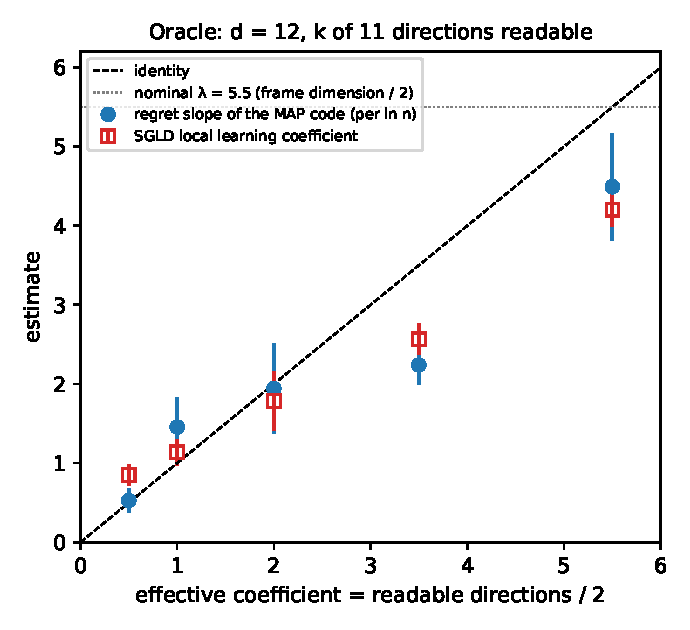
\includegraphics[width=0.6\textwidth]{../talk_slt/oracle_effective_coefficient.pdf}
\caption{The oracle with $k$ of 11 readable directions ($d=12$, $n=2048$): the MAP code's regret slope (Table~\ref{tab:ksweep}) and the SGLD local learning coefficient (step $10^{-4}$, localisation 10; Section~\ref{sec:ha3concl}) against $k/2$. Both track $k/2$ rather than the nominal 5.5 or the Bayes coefficient $k/2+(11-k)/4$ (3.0 to 5.5); Section~\ref{sec:coef:oracle} shows that the Bayes code of the same family follows the latter.}
\label{fig:oracleeff}
\end{figure}

\subsection{Readout sharpness and margin}
\label{sec:ha3sharp}

\paragraph{The double-noise pitfall.} The first attempt at a sharpness sweep exposed a misspecification that the earlier oracle runs had avoided by construction. The oracle's readout is the observed label law itself: its logit scale $\beta$ is set so that the readout's probability of the observed label equals the randomized-response law at the chosen noise rate (Section~\ref{sec:tb:synthetic}). If the learner applies its channel~\eqref{eq:channel} on top, the predictor codes a law that is noisier than the one generating the labels, and this double noise inflates the regret and its slope: at $d=6$, $k=5$ ($\lambda=2.5$) the matched readout without the channel has slope $3.39\pm0.31$ (regret 9.9 nats at $n=2048$) and with the channel $12.00\pm2.09$ (32.3 nats). All oracle regret figures in this section are therefore taken without the learner's channel unless the readout has been sharpened far enough that the channel is the only source of noise, and then the regret is measured against the oracle's own counterfactual law rather than the fixed randomized-response formula.

\paragraph{The $\pm1$ coordinate is trivially separable.} In the original oracle the $V$ coordinate takes the values $\pm1$, so no point lies near the decision boundary (the set of states at which the readout's two classes are equally likely). Sharpening the readout by a factor $10$ (multiplying $\beta$ by 10, with the channel) then gives a regret of exactly 0.0 nats and slope $0.00\pm0.00$: once the span is found no mistake is ever made. At a factor $100$ (and $1000$) the MAP fit fails, with slope $1024.61\pm23.22$ and a regret of 2644 nats, the vanishing-gradient collapse of a saturated readout (Section~\ref{sec:bayescode}). Neither outcome tests the law, so the sharpness study moved to a continuous $V$ coordinate.

\paragraph{Continuous $V$: a sharper readout raises the cost per $\ln n$.} With a continuous coordinate, $V\sim\mathcal N(0,1)$ instead of $\pm1$, points near the boundary exist and a sharpened readout is genuinely saturated there; the regret is measured against the oracle's own counterfactual law. At $d=6$, $k=5$ ($\lambda_{\mathrm{eff}}=\lambda=2.5$), $n=2048$: at the matched sharpness the corrected slope is $1.53\pm0.50$ without the channel (regret 10.0 nats) and $1.03\pm0.36$ with it (7.2 nats); with the channel at sharpness $\times3$, $\times10$, $\times30$ and $\times100$ the slopes are $1.26\pm0.25$, $2.09\pm0.56$, $6.53\pm0.84$ and $14.21\pm1.72$, with regrets 9.2, 20.4, 38.6 and 113.6 nats. Below sharpness $\times10$ the slope is of the order of $\lambda_{\mathrm{eff}}$; above it the cost per $\ln n$ grows with the sharpness, to six times $\lambda$ at $\times100$. The interpretation is that a small angular error in the fitted direction flips the predicted label of the points nearest the boundary, and a sharp readout flips them \emph{confidently}: each such point costs the channel floor, about 3 nats at the 10\% rate ($-\ln(\mathrm{rate}/2)$), rather than a fraction of a nat. These are hard mistakes whose number decreases with $n$ only as the angular error does, a pre-asymptotic regime in which the regret is governed not by the curvature count but by the number of boundary points times the floor.

\paragraph{Margin control.} If this reading is right, removing the boundary points should remove the excess. The continuous coordinate was resampled with a forbidden band $|v|<m$, at sharpness $\times10$ and $\times30$, six seeds. A margin of $0.3$ lowers the $\times30$ slope from $6.53\pm0.84$ to $2.70\pm1.24$ (per seed 0.0, 0.0, 6.7, 5.0, 4.5, 0.0; regret 34.5 nats), and at $\times10$ gives $4.56\pm1.37$ (per seed 1.4, 9.6, 3.9, 7.2, 4.5, 0.8; regret 23.4 nats).\footnote{A second comparison at $\times30$ with the channel and margins 0, 0.3 and 1.0 gave slopes $6.53\pm0.84$, $2.93\pm1.73$ and $508.28\pm292.52$; its seed count is not recorded.} A margin of $1.0$ at $\times10$ gives a seed-mean regret of 3.9 nats with per-seed final regrets of $0.7$, $2.7$, $19.8$, $0.0$, $0.0$, $0.0$ nats and per-seed slopes $0.21$, $-0.0$, $11.37$, $0.0$, $0.0$, $0.0$: on three of the six seeds the regret is exactly zero, on two more it is a few nats paid in the first blocks and flat afterwards, and one seed pays 19.8 nats. At $\times30$ with margin $1.0$ the six seeds split: three saturate at $5.8$, $14.7$ and $23.6$ nats (slopes 3.2, 0.0, 7.2), and three collapse to about 2700 nats ($2688$, $2709$, $2730$; slopes about 1000), which is the same vanishing-gradient failure of the MAP learner seen at $\times100$ with the $\pm1$ coordinate and on the saturated transformer readouts of Section~\ref{sec:bayescode}; the seed mean, $1361.8$ nats with slope $519\pm231$, is the average of two populations and means nothing by itself.

Where the fit does not collapse, then, a sharp readout with a margin pays a search cost and nothing after the span is found, the pattern the realizable InterpBench locus shows up to $n=1024$ in Table~\ref{tab:ha3ib}. The analogy was first taken to explain the InterpBench flatness. It does not hold beyond that range: the InterpBench flatness was the interpolation regime (Section~\ref{sec:ha3concl}).

\subsection{Beyond the interpolation regime: three regimes of the plug-in code}
\label{sec:ha3concl}

\paragraph{InterpBench with 8192 targets: the growth resumes.} The MAP subspace code of Section~\ref{sec:ha3ib:ib} (the same learner: 100 L-BFGS steps per block, warm start, prior precision 0.01, the 5\% channel, three seeds) was rerun on case~18 with the geometric schedule extended to 8192 targets, at $\dv=4$ and $\dv=1$. The 8192 targets are a new draw from the same pool with the same seed, not an extension of the 1024-target set (only the first 1024 base inputs coincide), and the regret is measured against the final fit on all 8192, so the block-end values are not those of Table~\ref{tab:ha3ib}; the slopes are batching-corrected least-squares fits against $\ln n$ on the block ends $n\ge64$ and $n\ge512$ (Table~\ref{tab:ha3ib8192}).

The regret of the valid alignment at \texttt{resid\_2} does not saturate. At $\dv=4$ the seed-mean regret at the block ends $n=16,32,\dots,8192$ is $7.8$, $15.2$, $19.3$, $34.8$, $42.2$, $60.9$, $71.2$, $83.5$, $115.8$ and $144.1$ nats, and the local slope per $\ln n$ between consecutive block ends is $10.6$, $5.9$, $22.4$, $10.6$, $27.0$, $14.9$, $17.7$, $46.6$, $40.9$: 10--27 nats per $\ln n$ up to $n=1024$, as in Table~\ref{tab:ha3ib}, and 41--47 over the last two doublings. The corrected slope is $16.8\pm2.8$ on $n\ge64$ and $21.1\pm1.7$ on $n\ge512$, against $8.4\pm2.9$ on the 1024-target run. At $\dv=1$ the block-end regrets are $16$, $41$, $64$, $94$, $113$, $138$, $192$, $208$, $245$ and $285$ nats with local slopes $36$, $33$, $43$, $28$, $36$, $78$, $23$, $54$, $57$, a corrected slope of $31.5\pm8.8$ on $n\ge64$ and $34.8\pm5.8$ on $n\ge512$, against $11.7\pm1.1$ before. The misspecified locus \texttt{resid\_1} grows much faster, as before ($90.9\pm18.4$ and $114.7\pm11.0$ on $n\ge64$; 684 and 876 nats at $n=8192$), from the excess-loss drift of Section~\ref{sec:ha3ib:ib}; the ordering by faithfulness is unchanged.

\begin{table}[t]
\centering
\footnotesize
\caption{The learning-coefficient hypothesis on InterpBench case~18 with 8192 targets under the MAP subspace code (three seeds): batching-corrected regret slopes against $\ln n$ on the block ends $n\ge64$ and $n\ge512$ (mean $\pm$ seed s.e.), the seed-mean regret at $n=8192$, the nominal $\lambda=\dv(d-\dv)/2$, and the slope of the 1024-target run (Table~\ref{tab:ha3ib}, $n\ge64$). The regret is against the final fit on all 8192 targets. \texttt{resid\_2} is the realizable locus, \texttt{resid\_1} the misspecified one.}
\label{tab:ha3ib8192}
\begin{tabular}{llrrrcr}
\toprule
$\dv$ & configuration & slope $n\ge64$ & slope $n\ge512$ & regret at $n{=}8192$ & $\lambda$ & slope, $n\le1024$ run \\
\midrule
4 & subspace at \texttt{resid\_2} & $16.8\pm2.8$ & $21.1\pm1.7$ & 144 & 512 & $8.4\pm2.9$ \\
4 & subspace at \texttt{resid\_1} & $90.9\pm18.4$ & $109.4\pm27.6$ & 684 & 512 & $106.9\pm14.7$ \\
\midrule
1 & subspace at \texttt{resid\_2} & $31.5\pm8.8$ & $34.8\pm5.8$ & 285 & 129.5 & $11.7\pm1.1$ \\
1 & subspace at \texttt{resid\_1} & $114.7\pm11.0$ & $144.7\pm11.5$ & 876 & 129.5 & $133.1\pm38.4$ \\
\bottomrule
\end{tabular}
\end{table}

\paragraph{The earlier flatness was the interpolation regime.} The explanation of the flat range is in the MAP's own training loss, which rises from $0.149$ nats per target on 1024 targets to $0.170$ on 8192. The $\dv=4$ frame has $260\cdot4=1040$ parameters against 1024 targets, so the 1024-target fits were partly interpolating, and the saturation read off Table~\ref{tab:ha3ib} was measured inside the interpolation regime, in which a map with more parameters than targets fits every prefix and the regret has no room to grow. This \emph{revises} the reading of Sections~\ref{sec:ha3ib:ib} and~\ref{sec:ha3sharp} that the regret at the realizable locus saturates once the span is found: it was flat in the range observed, up to $n=1024$, and the logarithmic growth resumes once $n$ exceeds the number of map parameters. Beyond $n\approx2000$ the data constrain the map and the regret at $\dv=4$ grows at roughly 45 nats per $\ln n$, which, read as a learning coefficient, means about 90 constrained directions: 9\% of the frame's parameters, far below the nominal $\lambda=512$, and more than the five to seven directions that carry 90\% of the empirical Fisher trace at the 1024-target fit (Section~\ref{sec:ha3eff}). The $\dv=1$ run is analogous (local slopes 54 and 57 over the last two doublings against a nominal 129.5). Whether the slope settles at this value cannot be read from two doublings, and the runs were extended to $n=32768$.

\paragraph{InterpBench with 32768 targets.} With the subspace map (same learner, three seeds; slopes on $n\ge64$, $\ge512$ and $\ge2048$; Table~\ref{tab:ha3ib32768}) the valid alignment's coefficient keeps rising slowly with the fit range: $22.6\pm4.1$, $27.1\pm5.7$ and $31.7\pm8.4$ at $\dv=4$ (against $8.4\pm2.9$ on the 1024-target run and $16.8\pm2.8$ on the 8192-target run, both on $n\ge64$), and $32.6\pm2.0$, $40.5\pm0.1$ and $42.0\pm0.0$ at $\dv=1$ (against $11.7\pm1.1$ and $31.5\pm8.8$). The 8192-target run's ``about 45 over the last doublings'' is thus confirmed as the local value beyond $n\approx2000$: with 1040 frame parameters the subspace family on InterpBench has a plug-in coefficient of roughly 30--40 on $n\in[2048,32768]$, 6--8\% of the nominal 512, consistent with GPT-2's 35--50 of 6016 (Section~\ref{sec:coef:scale}). Whether it settles is still open at this range. The misspecified locus is four to six times higher ($159\pm15$, $186\pm18$ and $178\pm20$ at $\dv=4$; $121\pm15$, $120\pm12$ and $135\pm17$ at $\dv=1$).

A methods note on these runs. The first 32768-target runs were launched with the InterpBench runner's default \emph{rotation} family instead of the subspace map. The rotation's warm-started L-BFGS MAP does not track across blocks: those runs returned regret slopes of about 1000--1250 at $n=32768$ with IIA 1.00, identical over seeds because the rotation's initialisation (the identity) does not depend on the seed. They are kept as a learner-failure note and not used. The same mistake affected the first HMC jobs of Section~\ref{sec:coef:gpt2}; both were rerun with the subspace map.

\begin{table}[t]
\centering
\footnotesize
\caption{The learning-coefficient hypothesis on InterpBench case~18 with 32768 targets under the MAP subspace code (three seeds): batching-corrected regret slopes against $\ln n$ on the block ends $n\ge64$, $n\ge512$ and $n\ge2048$ (mean $\pm$ seed s.e.), with the $n\ge64$ slopes of the 1024- and 8192-target runs (Tables~\ref{tab:ha3ib} and~\ref{tab:ha3ib8192}).}
\label{tab:ha3ib32768}
\begin{tabular}{llrrrrr}
\toprule
$\dv$ & configuration & $n\ge64$ & $n\ge512$ & $n\ge2048$ & 1024-target run & 8192-target run \\
\midrule
4 & subspace at \texttt{resid\_2} & $22.6\pm4.1$ & $27.1\pm5.7$ & $31.7\pm8.4$ & $8.4\pm2.9$ & $16.8\pm2.8$ \\
4 & subspace at \texttt{resid\_1} & $159\pm15$ & $186\pm18$ & $178\pm20$ & $106.9\pm14.7$ & $90.9\pm18.4$ \\
\midrule
1 & subspace at \texttt{resid\_2} & $32.6\pm2.0$ & $40.5\pm0.1$ & $42.0\pm0.0$ & $11.7\pm1.1$ & $31.5\pm8.8$ \\
1 & subspace at \texttt{resid\_1} & $121\pm15$ & $120\pm12$ & $135\pm17$ & $133.1\pm38.4$ & $114.7\pm11.0$ \\
\bottomrule
\end{tabular}
\end{table}

\paragraph{Three regimes of the MAP code.} The investigation leaves three regimes for the MAP subspace code, distinguished by the readout's sharpness and by whether the variable has mass near the decision boundary.
\begin{itemize}
\item \emph{Smooth readout, boundary mass.} The regret grows like $\lambda_{\mathrm{eff}}\ln n$, where $\lambda_{\mathrm{eff}}$ counts half the directions the readout responds to and not the dimension of the Grassmannian (Table~\ref{tab:ksweep}: slopes $0.53$ to $4.49$ for $k/2$ from $0.5$ to $5.5$ at a nominal 5.5). This is the plug-in code's coefficient; the Bayes code of the same family reads $1.98$ to $4.72$ on the same sweep, and $3.05$ to $5.43$ with 16384 targets, against its learning coefficient $k/2+(11-k)/4$ from $3.0$ to $5.5$ (Section~\ref{sec:coef:oracle}).
\item \emph{Sharp readout, boundary mass.} The cost per $\ln n$ rises above $\lambda_{\mathrm{eff}}$, to $14.2\pm1.7$ against $2.5$ at sharpness $\times100$, because the boundary points flip confidently at the channel floor: a pre-asymptotic regime of hard mistakes, not a learning coefficient. The Bayes code's own coefficient also rises there, from $2.4$ to $5.3$, i.e.\ from $k/2$ to $k$, as a one-dimensional quadrature predicts; the MAP code's $14.2$ is two to three times that, a learner excess (Section~\ref{sec:coef:oracle}). With 16384 targets the Bayes coefficient at $\times100$ falls back to $3.55\pm0.47$ while the MAP code's stays at $10.34\pm4.49$: the Bayes code's excess is a finite-$n$ crossover, the MAP code's a learner effect that persists.
\item \emph{Sharp readout with a margin}, the situation of discrete tokens. The regret saturates once the span is found (exact zeros on three of six seeds at $\times10$; 6 to 24 nats on the seeds whose fit survives at $\times30$), and a MAP learner on such a readout can also fail outright by vanishing gradients.
\end{itemize}
Up to $n=1024$ the trained transformer looked like the last case with few readable directions (five to seven dominant of 1024 at the realizable InterpBench locus), and its regret was both flat and small. The runs with 8192 and 32768 targets show that this flatness was the interpolation regime of the map and not saturation; what remains of the first reading is that the coefficient at which the growth resumes is a small fraction of the nominal one.

\paragraph{A direct estimate of the learning coefficient is unstable on the transformer.} The regret slope is one estimator of the effective coefficient; the local learning coefficient of singular learning theory is another, and a stochastic-gradient Langevin (SGLD) estimator of it was built to cross-check the first: a tempered posterior\footnote{A \emph{tempered} posterior at inverse temperature $\beta$ has density proportional to the prior times the likelihood raised to the power $\beta$; for $\beta<1$ it is flatter than the posterior. \emph{Localisation} adds a quadratic penalty $\tfrac{\gamma}{2}\|w-w^*\|^2$ to the energy, which keeps the samples near the point $w^*$ at which the coefficient is to be estimated.} at $\beta=1/\ln n$, localised at the MAP with a strength given in units of each tensor's scale, four chains, and $\hat\lambda=n\beta\,(\mathbb{E}[L_n]-L_n^*)$ with the expectation over the second half of each chain \cite{lau2025llc}. On the oracle $k$-sweep of Table~\ref{tab:ksweep} ($d=12$, $n=2048$; step $10^{-4}$, localisation 10, 1000 steps) it reads $0.85\pm0.13$, $1.14\pm0.17$, $1.78\pm0.37$, $2.57\pm0.19$ and $4.20\pm0.21$ for $k=1,2,4,7,11$, against $\lambda_{\mathrm{eff}}=k/2$ from $0.5$ to $5.5$ and regret slopes from $0.53$ to $4.49$: the two estimators agree with each other and with $k/2$ to within 20--30\%, while a smaller step or a tighter localisation under-mixes and underestimates (0.1 to 1.5 in the same sweep).

On the InterpBench transformer the same estimator is not stable. At the fitted $\dv=4$ subspace on \texttt{resid\_2} ($n=1024$ targets, training loss $0.149$ nats per target) it reads $0.96\pm0.69$ with step $10^{-4}$, localisation 10 and 1000 steps; $12.65\pm12.32$ with 2000 steps, one chain drifting to 49.6; $27.36\pm13.94$ at step $10^{-3}$, with chains at 23.6, 66.9, 17.1 and 1.9; and $2.22\pm0.18$ under tight localisation (strength 1), the only stable reading, whose value is then set by the localiser as much as by the landscape. At the misspecified locus \texttt{resid\_1} the same four settings give $6.39\pm0.99$, $18.22\pm2.75$, $64.90\pm14.28$ and $13.03\pm1.94$. The growth with chain length and with step size says that the chains are drifting along the flat directions of the saturated readout rather than equilibrating, and that the localisation does not confine them within 1000--2000 steps. What the estimator reproduces is the ordering, the misspecified locus higher in every setting as its regret slope is, and the order of magnitude at the valid locus, a few readable directions against the five to seven of the Fisher spectrum; what it does not reproduce is the number. The LLC is therefore reported as a diagnostic together with its sensitivity and not as a summary column, and the regret slope of the MAP code remains our estimator of the code's coefficient.

The per-chain loss traces confirm this reading: in no setting does a chain reach a plateau. At the valid locus with step $10^{-4}$ and localisation 10, three chains sit at $0.0$--$0.8$ for all 2000 steps while the fourth leaves the flat region after about 600 steps and grows without bound ($4.5$ to $85$ between steps 800 and 1800); with localisation 1 all four grow steadily from 0 to $7$--$21$; at step $10^{-5}$ nothing moves. The loss is exactly flat around the MAP over the localisation scale, since moving the span changes no prediction until a target crosses the decision boundary, so the tempered posterior at $\beta=1/\ln n$ is not a local object at this $n$, and the sampler measures the extent and the boundary of the flat region rather than a power law at a point. On a MAP fitted to 8192 targets the same pathology is stronger, the drift term being six times larger: $88\pm36$ at step $10^{-4}$ (two chains near 0, two escaping to $160$--$220$), $0.01$ at $10^{-5}$, $173\pm50$ with localisation 100, no setting near the regret slope of 17--45. On reduced-rank regression, where $\lambda$ is known, the same estimator reads it (Section~\ref{sec:coef:rrr}), on the oracle it tracks $k/2$ (Figure~\ref{fig:oracleeff}), and Section~\ref{sec:coef} explains why, even if it converged, it would not return the regret slope on the trained testbeds: the two measure different coefficients there.

\section{Learner coefficients, Bayes coefficients and the information equality}
\label{sec:coef}

Every slope in Section~\ref{sec:ha3ib} is the regret slope of the MAP subspace code: the cumulative excess of one predictor sequence, the L-BFGS fit on each prefix, over the final fit on the same targets, per $\ln n$. It is a \emph{learner coefficient} $\kappa$ (Section~\ref{sec:regretdef}), and singular learning theory describes it only through a comparison with the Bayes learning coefficient $\lambda$ of the family, which is the coefficient of the Bayes predictive \cite{watanabe2009}. Our research plan lists this comparison as an open question: ``Conditions under which a learner's coefficient $\kappa$ equals $\lambda$, and singular families in which plug-in predictors have $\kappa\neq\lambda$.'' Section~\ref{sec:ha3ib} read its slopes as effective learning coefficients without making the distinction. This section makes it, on three testbeds in order of decreasing control, and finds that it decides the interpretation of everything measured so far.

In reduced-rank regression, where $\lambda$ is known exactly, the Bayes code's slope is $\lambda$ and the plug-in's is the regular $MN/2$ (Section~\ref{sec:coef:rrr}). On the oracle, where a genuine Bayes code of the subspace map can be run by Hamiltonian Monte Carlo (HMC) next to the MAP code, the two coefficients differ in both directions, and the Hessian and the Fisher at the MAP say why; with 16384 targets the Bayes code's slope reaches the family's learning coefficient $k/2+(d-1-k)/4$, which counts the directions the data do not occupy at $1/4$ each (they are quartic, not flat), and the plug-in's stays at $k/2$ (Section~\ref{sec:coef:oracle}). On GPT-2 the same mechanism is a hundredfold stronger: the subspace family is regular on its Grassmannian with the nominal coefficient 6016, the Fisher is two per cent of the Hessian, the plug-in's coefficient is predicted at 71 from the two matrices and measured at 45--50, and a genuine Bayes code of the valid InterpBench alignment is longer than the label-only code at 1024 targets (Section~\ref{sec:coef:gpt2}); across subspace dimensions 4 to 64 the plug-in's coefficient stays at 49--79 while the nominal Bayes coefficient grows fifteenfold. On hierarchical equality, where the nominal coefficient is 56, a genuine Bayes code is the shorter one, which places the three trained testbeds on a ladder in $n$ against $\lambda$ (Section~\ref{sec:coef:ladder}). Section~\ref{sec:coef:scale} gives the scale dependence of the plug-in's coefficient to 32768 targets on both trained testbeds, and Section~\ref{sec:coef:consequences} states what follows for the score and how it revises the wording of Section~\ref{sec:ha3eff}.

\paragraph{Notation.} Throughout, $H$ is the Hessian of the mean loss at the MAP, and $F$ the \emph{empirical Fisher} there: the mean outer product of the per-example gradients, i.e.\ their uncentred second moment. (An earlier version of this analysis described $F$ as the covariance of the per-example gradients; the computation does not subtract the mean gradient. The two differ by the outer product of the mean gradient, which is small where the MAP is close to stationary.) The two predictions set against the measured slopes are the plug-in's $\tfrac12\,\mathrm{tr}(FH^{-1})$ (with the pseudo-inverse on the gauge directions) and, for a Bayes code at finite $n$, the Laplace count $\tfrac12\sum_i n h_i/(n h_i+\alpha)$ over the eigenvalues $h_i$ of $H$ with prior precision $\alpha$, which tends to half the number of curved directions once $n$ resolves them all. The plug-in prediction assumes the exact minimiser on every prefix. The two agree when $F=H$, the information equality of a correctly specified regular model; what the subsections below measure is where it fails.

\subsection{The exact example: reduced-rank regression}
\label{sec:coef:rrr}

\paragraph{Family and codes.} The family is $y=UVx+e$ with $U$ of size $M\times H$ and $V$ of size $H\times N$, unit Gaussian inputs and noise, an $\mathcal N(0,1)$ prior on every entry, and a true law of rank $r$ (Section~\ref{sec:tb:synthetic}); its learning coefficient $\lambda$ and multiplicity $m$ are those of Aoyagi and Watanabe \cite{aoyagiwatanabe2005}, and the regular count is $MN/2$. Three codes were run on the same data: the Bayes code by HMC on the sufficient statistics (64 chains of 200 samples per block, 300 warm-up iterations, thinning 2), the least-squares plug-in code, and a Langevin estimate of the local learning coefficient at the MAP. The regret is against the true law, the schedule is geometric with ratio 2 from 8 to $n=65536$, the slopes are batching-corrected least-squares fits on $n\ge256$, and there are 16 seeds.

\begin{table}[t]
\centering
\footnotesize
\caption{Reduced-rank regression, $n=65536$, 16 seeds: the Aoyagi--Watanabe coefficient $\lambda$ and multiplicity $m$ of the family $(M,N,H,r)$, the regular count $MN/2$, and the batching-corrected regret slopes on $n\ge256$ of the least-squares plug-in code and of the Bayes code by HMC (mean $\pm$ s.e.\ over seeds). The plug-in slope is the same number for every $H$ and $r$ at fixed $(M,N)$. The lower block is the rank-restricted families run for the between-family gains.}
\label{tab:rrr}
\begin{tabular}{lrrrrr}
\toprule
$(M,N,H,r)$ & $\lambda$ & $m$ & $MN/2$ & plug-in slope & Bayes slope \\
\midrule
(2,2,2,2) & 2.0 & 1 & 2.0 & $2.11\pm0.18$ & $2.09\pm0.19$ \\
(2,2,2,0) & 1.5 & 1 & 2.0 & $2.11\pm0.18$ & $1.53\pm0.15$ \\
(3,3,3,0) & 3.5 & 2 & 4.5 & $4.31\pm0.26$ & $3.05\pm0.21$ \\
(3,3,3,1) & 4.0 & 1 & 4.5 & $4.31\pm0.26$ & $3.72\pm0.23$ \\
(4,4,4,0) & 6.0 & 1 & 8.0 & $8.29\pm0.31$ & $6.04\pm0.27$ \\
(4,4,4,2) & 7.5 & 1 & 8.0 & $8.29\pm0.31$ & $7.58\pm0.29$ \\
(4,2,4,0) & 3.5 & 1 & 4.0 & $3.81\pm0.17$ & $3.22\pm0.16$ \\
\midrule
(3,3,1,1) & 2.5 & 1 & 4.5 & $4.31\pm0.26$ & $2.48\pm0.15$ \\
(4,4,2,2) & 6.0 & 1 & 8.0 & $8.29\pm0.31$ & $6.06\pm0.23$ \\
(4,4,1,1) & 3.5 & 1 & 8.0 & $8.29\pm0.31$ & $3.51\pm0.15$ \\
(4,4,4,1) & 7.0 & 2 & 8.0 & $8.29\pm0.31$ & $6.91\pm0.27$ \\
(4,4,1,0) & 2.0 & 2 & 8.0 & $8.29\pm0.31$ & $1.99\pm0.20$ \\
\bottomrule
\end{tabular}
\end{table}

\paragraph{Bayes slope equals $\lambda$, plug-in slope equals $MN/2$.} Table~\ref{tab:rrr} answers the learner-versus-Bayes question numerically for this family. The Bayes code's coefficient is the Aoyagi--Watanabe $\lambda$ on all twelve shapes, to within one standard error on most of them ($2.09\pm0.19$ for $\lambda=2$, $1.53\pm0.15$ for $1.5$, $6.04\pm0.27$ for 6, $7.58\pm0.29$ for $7.5$, $3.51\pm0.15$ for $3.5$, $1.99\pm0.20$ for 2) and within about two on the rest ($3.72\pm0.23$ for 4, $3.22\pm0.16$ for $3.5$). The shape $(3,3,3,0)$ with multiplicity $m=2$ sits $0.45$ below its $\lambda=3.5$ (and $(4,4,4,1)$, also $m=2$, $0.09$ below 7), which we attribute to the sign and, at these $n$, the size of the $-(m-1)\ln\ln n$ term. The plug-in's coefficient is the regular $MN/2$ whatever the true rank: $2.11\pm0.18$ against $2.0$, $4.31\pm0.26$ against $4.5$, $8.29\pm0.31$ against $8$, $3.81\pm0.17$ against $4$. Whenever the true rank is deficient the two codes have different coefficients, and the gap $MN/2-\lambda$ (0.5 for $(2,2,2,0)$, 1.0 for $(3,3,3,0)$, 2.0 for $(4,4,4,0)$, 0.5 for $(3,3,3,1)$, $(4,4,4,2)$ and $(4,2,4,0)$) is the predicted one within the errors. This is the clean form of the statement the rest of the section finds on the alignment families: the plug-in pays a regular count for the parameters it fits, the Bayes code pays the singular $\lambda$ of the family, and the two coincide only at full rank.

\paragraph{Gains between two families on the same data grow like $\Delta\lambda\ln n$.} The learning-coefficient hypothesis is a statement about the \emph{gain} between two configurations that both contain the truth. On the same data the Bayes code of a rank-restricted family was compared with that of the full family (Table~\ref{tab:rrr}, lower block against the matching upper rows), and the regret difference was fitted against $\ln n$ on $n\ge256$ over 16 seeds: for $(3,3,1,1)$ against $(3,3,3,1)$ the predicted $\Delta\lambda=1.5$ and the measured gain slope $1.23\pm0.15$; for $(4,4,2,2)$ against $(4,4,4,2)$, $1.5$ and $1.52\pm0.13$; for $(4,4,1,1)$ against $(4,4,4,1)$, $3.5$ and $3.40\pm0.21$ (multiplicities 1 and 2); for $(4,4,1,0)$ against $(4,4,4,0)$, $4.0$ and $4.05\pm0.14$ (multiplicities 2 and 1). Three of the four are within one standard error of $\Delta\lambda$; the first is $1.8$ s.e.\ below. On this family, where $\lambda$ is known, the hypothesis holds for the Bayes code.

\paragraph{The batching correction holds for a singular Bayes code.} The batching correction of Section~\ref{sec:regretdef}, the factor $(r-1)/\ln r$ by which geometric blocks of ratio $r$ multiply the logarithmic coefficient of a learner with expected excess loss $\kappa/m$ after $m$ examples, was derived in our research plan and checked exactly there for the Gaussian mean, a regular family. On reduced-rank regression ($n=4096$, 8 seeds, slopes on $n\ge128$) the corrected Bayes slopes under per-sample coding, doubling blocks and quadrupling blocks are $3.15$ / $3.13$ / $2.84$ for $(3,3,3,0)$, $5.75$ / $6.00$ / $6.24$ for $(4,4,4,0)$, $2.11$ / $1.94$ / $1.98$ for $(2,2,2,2)$ and $7.18$ / $7.44$ / $7.68$ for $(4,4,4,2)$, with standard errors between $0.25$ and $1.0$: the three schedules agree after the correction, for a singular family and not only for the regular one.

\paragraph{The Langevin local learning coefficient.} At $n=4096$ the estimator at the MAP (step $10^{-4}$, pull 1, 4000 steps) reads $3.38$, $6.25$, $2.16$ and $7.91$ for $\lambda=3.5$, $6$, $2$ and $7.5$. At $n=65536$ the same step overshoots or diverges ($9.40\pm0.07$ for $\lambda=2$; non-finite for the $4\times4$ shapes), because the drift $n\beta\nabla L$ grows with $n$ and the step has to shrink with it; the LLC is reported at $n=4096$ only. On a family where $\lambda$ is known, then, the sampler reads it, with the usual sensitivity to the step; its failure on the InterpBench transformer (Section~\ref{sec:ha3concl}) is not a failure of the estimator as such.

\subsection{The oracle: Bayes and MAP coefficients, sharp readouts and quartic directions}
\label{sec:coef:oracle}

\paragraph{A genuine Bayes code by HMC.} The MAP subspace code of Sections~\ref{sec:ha3eff} and~\ref{sec:ha3sharp} was run again on the same oracle settings next to a Bayes code of the subspace map: a Gaussian prior $\mathcal N(0,1)$ on the raw frame, HMC with four chains of 100 samples after 200 warm-up iterations, ten leapfrog steps,\footnote{HMC moves a sample by simulating Hamiltonian dynamics in which the negative log posterior is the potential energy; a \emph{leapfrog step} is one step of the symplectic integrator used for the simulation, and a Metropolis test at the end of each trajectory corrects the discretisation error \cite{neal2011hmc}.} the step size adapted during warm-up towards an acceptance rate of about 0.7 (it is multiplied by 1.05 on acceptance and by 0.9 on rejection, which equilibrates at about 0.68), and chains that continue across blocks; the predictor on each block is the average of the sampled maps' predictive distributions. The regret is against the oracle's own law, the schedule is geometric with ratio $1.25$ from 16, the batching-corrected slope is fitted on $n\in[256,2048]$, four seeds. Table~\ref{tab:oraclebayes} gives both coefficients for the sharpness sweep ($d=6$, $k=5$ readable directions, continuous $V$, channel 0.1, $\lambda_{\mathrm{eff}}=k/2=2.5$) and for the $k$-sweep ($d=12$, sharpness $\times1$, no channel); Figure~\ref{fig:oraclebayes} plots them.

\begin{table}[t]
\centering
\footnotesize
\caption{The oracle: batching-corrected regret slopes per $\ln n$ on $n\in[256,2048]$ of the MAP subspace code (the learner coefficient $\kappa$) and of the Bayes code by HMC ($\lambda$), four seeds; HMC acceptance 0.48--0.79. Left: sharpness sweep at $d=6$, $k=5$, continuous $V$, randomized-response channel 0.1 ($k/2=2.5$; the first row is without the learner's channel). Right: $k$-sweep at $d=12$, sharpness $\times1$, no channel, with the Bayes learning coefficient $k/2+(11-k)/4$, the plug-in prediction $\tfrac12\mathrm{tr}(FH^{+})$ and the Laplace count (averaged over $n=256$ to 2048, prior precision 1) from the Hessian and empirical Fisher at the MAP; the Laplace count mis-models the $11-k$ quartic directions and is superseded by the learning coefficient (see text).}
\label{tab:oraclebayes}
\resizebox{\textwidth}{!}{%
\begin{tabular}{lrrrrrrrrr}
\toprule
sharpness & MAP ($\kappa$) & Bayes ($\lambda$) & $k$ & $k/2$ & $k/2+\tfrac{11-k}{4}$ & MAP ($\kappa$) & Bayes ($\lambda$) & $\tfrac12\mathrm{tr}(FH^{+})$ & Laplace count \\
\midrule
$\times1$, no channel & $1.53\pm0.50$ & $2.28\pm0.53$ & 1 & 0.5 & 3.00 & $0.53\pm0.15$ & $1.98\pm0.26$ & 1.10 & 1.33 \\
$\times1$ & $1.03\pm0.36$ & $2.40\pm0.35$ & 2 & 1.0 & 3.25 & $1.46\pm0.38$ & $2.88\pm0.46$ & 1.08 & 4.29 \\
$\times3$ & $1.26\pm0.25$ & $2.44\pm0.32$ & 4 & 2.0 & 3.75 & $1.94\pm0.57$ & $3.16\pm0.83$ & 2.41 & 3.29 \\
$\times10$ & $2.09\pm0.56$ & $2.95\pm0.57$ & 7 & 3.5 & 4.50 & $2.24\pm0.25$ & $3.19\pm0.41$ & 3.26 & 5.37 \\
$\times30$ & $6.53\pm0.84$ & $4.41\pm0.60$ & 11 & 5.5 & 5.50 & $4.49\pm0.68$ & $4.72\pm0.68$ & 4.47 & 5.49 \\
$\times100$ & $14.21\pm1.72$ & $5.32\pm0.59$ & & & & & & & \\
\bottomrule
\end{tabular}}
\end{table}

\begin{figure}[htbp]
\centering
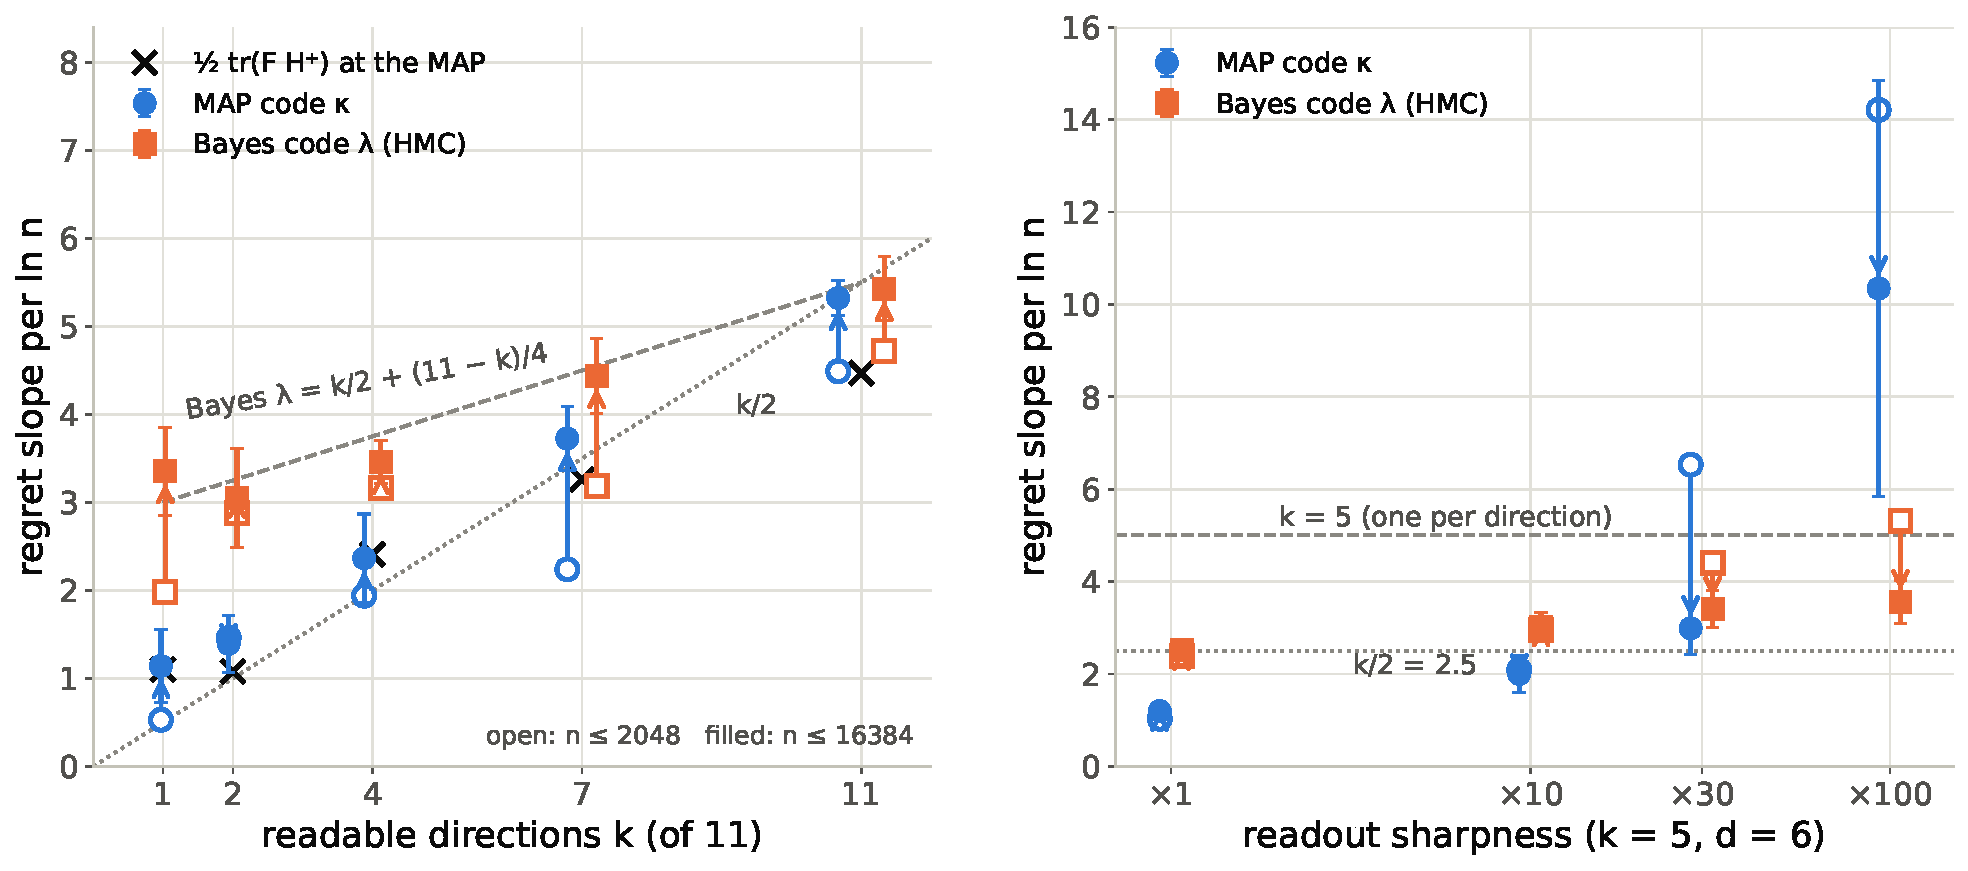
\includegraphics[width=\textwidth]{../talk_slt/oracle_kappa_vs_lambda.pdf}
\caption{The oracle, MAP code (circles, $\kappa$) against Bayes code by HMC (squares), slopes on $n\le2048$ (open; Table~\ref{tab:oraclebayes}) and on $n\le16384$ (filled; Table~\ref{tab:oracle16384}), with arrows from the first to the second; four seeds. Left: $k$-sweep at $d=12$, with the Bayes learning coefficient $k/2+(11-k)/4$ (dashed), $k/2$ (dotted) and $\tfrac12\mathrm{tr}(FH^{+})$ at the MAP (crosses). The MAP code follows $k/2$ and $\tfrac12\mathrm{tr}(FH^{+})$; the Bayes code is below its learning coefficient on $n\le2048$ and reaches it on $n\le16384$. Right: sharpness sweep at $d=6$, $k=5$, with $k/2=2.5$ (dotted) and $k=5$ (dashed); on $n\le2048$ the Bayes coefficient rises from $k/2$ to $k$ and the MAP code's to two to three times that; on $n\le16384$ the Bayes coefficient falls back towards $k/2$ and the MAP code's stays large at $\times100$ (sharpness $\times3$, not repeated at 16384 targets, is not shown).}
\label{fig:oraclebayes}
\end{figure}

\paragraph{Sharp readouts: the Bayes coefficient goes from $k/2$ to $k$, and the MAP code overshoots it.} Under the sharpness sweep the Bayes coefficient rises from $2.28\pm0.53$ and $2.40\pm0.35$ at $\times1$, the smooth value $k/2=2.5$, through $2.95\pm0.57$ at $\times10$ and $4.41\pm0.60$ at $\times30$ to $5.32\pm0.59$ at $\times100$, which is $k=5$: one per decision-relevant direction. This is what a one-parameter quadrature predicts. For $P(y=1\mid x)=(1-\varepsilon)\,\sigma(s(x-w))+\varepsilon/2$ with $x\sim\mathcal N(0,1)$, $\varepsilon=0.1$ and true $w_0=0$, the population KL divergence $K(w)$ is quadratic for $|w|\ll1/s$ and linear for $|w|\gg1/s$, so the local slope of the free energy $F_n=-\log\int e^{-nK(w)}\,dw$ against $\ln n$ is $1/2$ throughout for $s\le10$, starts at $0.71$ for $s=100$ and reaches $1/2$ by $n=2^{10}$, starts at $0.95$ for $s=1000$ and reaches $1/2$ only beyond $2^{14}$, and stays near 1 to $2^{14}$ for $s=10^4$; the crossover grows roughly like $s^{1.3}$. The asymptotic coefficient of the analytic sigmoid model is $1/2$ per direction; the value near 1 is a finite-$n$, scale-dependent coefficient, and $n\le2048$ with $k=5$ is the regime in which the Bayes slope should lie between $2.5$ and $5$, which it does. The MAP code's $6.53\pm0.84$ at $\times30$ and $14.21\pm1.72$ at $\times100$ (Section~\ref{sec:ha3sharp}) are therefore not $\lambda$ at any $n$: they are the learner's own coefficient, two to three times the Bayes code's, the price of a point estimate in a sharp landscape ($\kappa>\lambda$). Below $\times10$ the MAP code pays slightly \emph{less} than the Bayes code ($1.0$--$2.1$ against $2.4$--$3.0$).

\paragraph{Readable and quartic directions: the Bayes coefficient does not follow $k/2$.} Under the $k$-sweep the MAP code follows $k/2$ ($0.53$ to $4.49$, Table~\ref{tab:ksweep}), but the Bayes code does not: it reads $1.98\pm0.26$ at $k=1$ where $k/2=0.5$, and grows to $4.72\pm0.68$ at $k=11$. The directions of the frame outside the data's $(k+1)$-dimensional subspace are not flat for the Bayes code: a frame tilted by $\phi$ towards one of them swaps $\cos^2\!\phi$ of the difference in $V$, so the population loss grows as $\phi^4$ there (Section~\ref{sec:tb:synthetic}). They are quartic, with Fisher information and population Hessian both zero, and a quartic direction has learning coefficient $1/4$ (the volume of $\{\phi^4<\epsilon\}$ in $m$ such directions scales as $\epsilon^{m/4}$), a readable one $1/2$; the Bayes learning coefficient is $\lambda=k/2+(11-k)/4$, from $3.0$ at $k=1$ to $5.5$ at $k=11$, and on $n\le2048$ the measured Bayes slopes are below it at every $k$. The empirical minimiser sits at zero in the quartic directions on every sample, since no example favours a nonzero component, so the plug-in has no sampling variance there and pays nothing.

The Hessian and the empirical Fisher at the MAP of the $\dv=1$ map ($d=12$, $n=2048$, prior precision 1) show exactly this. The tangent-space Hessian has 11 positive eigenvalues for every $k$: $k$ large ones ($0.8$--$1.1$); one weakly curved extra direction at $k=1$ ($h=0.064$) and at $k=4$ ($h=0.15$), whose Fisher equals its Hessian; and in the remaining directions ($10-k$ at $k=1$ and 4, $11-k$ at $k=2$ and 7) small eigenvalues, identical across those directions: $9\times10^{-5}$, $0.004$, $4\times10^{-4}$ and $0.03$ at $k=1$, 2, 4 and 7. The small eigenvalues are not population curvature. With the population loss $K\approx a|\phi_r|^2+c(|\phi_r|^2+|\phi_e|^2)^2$ in the readable components $\phi_r$ and the unreadable $\phi_e$ of the tilt, $\partial^2K/\partial\phi_e^2=4c|\phi_r|^2$: the cross term, evaluated at a MAP whose readable components carry sampling error, which vanishes as $n$ grows. The Fisher in the large and extra directions is of the same size as the Hessian ($F_{ii}/h_i$ between 0.65 and 1.2) and in the small ones $10^{-16}$ (at most $2\times10^{-6}$). The plug-in prediction $\tfrac12\mathrm{tr}(FH^{+})$ is $1.1$, $1.1$, $2.4$, $3.3$, $4.5$ for $k=1,2,4,7,11$ against the measured MAP slopes $0.53$, $1.46$, $1.94$, $2.24$, $4.49$ (the $k=1$ value is low because the weakly curved second direction, $h=0.064$, is not resolved by 100 warm-started L-BFGS steps per block). The Laplace count built on these eigenvalues, averaged over $n=256$ to 2048, is $1.3$, $4.3$, $3.3$, $5.4$, $5.5$ against the measured Bayes slopes $2.0$, $2.9$, $3.2$, $3.2$, $4.7$. It mis-models the directions with small eigenvalues: a Gaussian approximation counts each at $0$ or $\tfrac12$ according to whether $nh$ is below or above 1, whereas they are quartic and count $\tfrac14$ at any $n$, and their $h$ is a sampling artefact of the MAP. The Laplace count is therefore superseded by $\lambda=k/2+(11-k)/4$.

The plug-in's prequential coefficient $\tfrac12\mathrm{tr}(FH^{+})=k/2$ is thus below the Bayes learning coefficient, which counts every direction in which the population loss rises, whatever $F$: at $\tfrac12$ in the readable directions, where $F=H$, and at $\tfrac14$ in the deterministically constrained ones, where $F$ and $H$ both vanish in the population and the loss is quartic. The statement ``$\lambda_{\mathrm{eff}}=k/2$'' of Section~\ref{sec:ha3eff} describes the plug-in code: the Bayes coefficient of the subspace family on this oracle is $k/2+(d-1-k)/4$, between $k/2$ and the nominal $(d-1)/2$ and equal to the latter only at $k=d-1$ (Table~\ref{tab:oracle16384}). Three regimes of the relation between the learner's coefficient and the Bayes coefficient are now measured: $\kappa_{\mathrm{MAP}}<\lambda$ on smooth, deterministically constrained families; $\kappa_{\mathrm{MAP}}>\lambda$ on sharp readouts; $\kappa_{\mathrm{OLS}}>\lambda$ for the least-squares plug-in in reduced-rank regression.

\paragraph{To 16384 targets: the Bayes coefficient approaches its $\lambda$, the plug-in's stays at $k/2$.} Both sweeps were repeated with 16384 targets (four seeds, slopes on $n\in[256,16384]$; Table~\ref{tab:oracle16384}, Figure~\ref{fig:oraclebayes}). In the $k$-sweep the Bayes slope reaches $\lambda=k/2+(11-k)/4$ at every $k$: $3.35\pm0.50$, $3.05\pm0.56$, $3.46\pm0.24$, $4.44\pm0.43$ and $5.43\pm0.36$ for $k=1$, 2, 4, 7 and 11 against $3.0$, $3.25$, $3.75$, $4.5$ and $5.5$, within $0.7$ seed standard errors at $k=1$, 2, 7 and 11 and $1.2$ at $k=4$. The movement from $n\le2048$, where the slopes ($1.98$ to $4.72$) are below $\lambda$ at every $k$, is the finite-$n$ approach to the asymptotic coefficient; at $k=1$ the value $3.35$ is the quartic count $3.0$, not a step towards the nominal $5.5$. A decisive test is running: a Bayes code by HMC at 65536 targets for $k=1$, 4 and 7 with slopes on $n\ge1024$, where $\lambda$ predicts $3.0$, $3.75$ and $4.5$ and a coefficient tending to the nominal value would give $5.5$. The plug-in's coefficient stays near $\tfrac12\mathrm{tr}(FH^{-1})$: $1.14\pm0.42$ at $k=1$ is the predicted $1.1$ (the weakly curved extra direction, $h=0.064$, which 100 L-BFGS steps per block did not resolve on $n\le2048$, is resolved at this $n$), and the values at $k=7$ and 11, $3.73$ and $5.32$, are the readable count over two within the errors. In the sharpness sweep the Bayes coefficient at $\times100$ falls from $5.32$ back to $3.55\pm0.47$, towards $k/2$ and still above it, and at $\times1$ it is $2.51\pm0.08$, $k/2$ to the second decimal. The sharp-readout excess of the Bayes code is thus the finite-$n$ crossover of the one-dimensional quadrature, resolved once $n$ exceeds roughly $s^{1.3}$. The MAP code's coefficient at $\times30$ falls from $6.53$ to $2.99\pm0.57$, but at $\times100$ it stays large, $10.34\pm4.49$, with a seed-to-seed spread of the same size: in a sharp landscape the plug-in's excess is a learner effect that does not go away with $n$.

\begin{table}[t]
\centering
\footnotesize
\caption{The oracle with 16384 targets: batching-corrected regret slopes per $\ln n$ of the MAP subspace code ($\kappa$) and of the Bayes code by HMC ($\lambda$), four seeds, fitted on $n\in[256,2048]$ (from Table~\ref{tab:oraclebayes}) and on $n\in[256,16384]$. Upper block: sharpness sweep at $d=6$, $k=5$, continuous $V$, channel 0.1 ($k/2=2.5$; sharpness $\times3$ was not repeated). Lower block: $k$-sweep at $d=12$, sharpness $\times1$, no channel. Last column: the asymptotic Bayes learning coefficient, $k/2=2.5$ in the sharpness sweep (one half per direction for the analytic sigmoid) and $k/2+(11-k)/4$ in the $k$-sweep.}
\label{tab:oracle16384}
\begin{tabular}{lrrrrr}
\toprule
 & MAP, $n\le2048$ & MAP, $n\le16384$ & Bayes, $n\le2048$ & Bayes, $n\le16384$ & $\lambda$\\
\midrule
sharpness $\times1$ & $1.03$ & $1.20\pm0.05$ & $2.40$ & $2.51\pm0.08$ & 2.5\\
sharpness $\times10$ & $2.09$ & $2.00\pm0.39$ & $2.95$ & $3.03\pm0.31$ & 2.5\\
sharpness $\times30$ & $6.53$ & $2.99\pm0.57$ & $4.41$ & $3.41\pm0.40$ & 2.5\\
sharpness $\times100$ & $14.21$ & $10.34\pm4.49$ & $5.32$ & $3.55\pm0.47$ & 2.5\\
\midrule
$k=1$ ($k/2=0.5$) & $0.53$ & $1.14\pm0.42$ & $1.98$ & $3.35\pm0.50$ & 3.00\\
$k=2$ ($1.0$) & $1.46$ & $1.39\pm0.32$ & $2.88$ & $3.05\pm0.56$ & 3.25\\
$k=4$ ($2.0$) & $1.94$ & $2.37\pm0.50$ & $3.16$ & $3.46\pm0.24$ & 3.75\\
$k=7$ ($3.5$) & $2.24$ & $3.73\pm0.37$ & $3.19$ & $4.44\pm0.43$ & 4.50\\
$k=11$ ($5.5$) & $4.49$ & $5.32\pm0.20$ & $4.72$ & $5.43\pm0.36$ & 5.50\\
\bottomrule
\end{tabular}
\end{table}

\subsection{The language model: the full Hessian and Fisher of the subspace loss}
\label{sec:coef:gpt2}

\paragraph{Spectrum.} The dense Hessian of the learned $\dv=16$ subspace's mean loss on GPT-2 IOI at layer~11 (12288 frame parameters, 1024 targets, prior precision 0.01, the MAP of 100 L-BFGS steps) was computed from 12288 Hessian-vector products\footnote{A \emph{Hessian-vector product} $Hv$ is computed by automatic differentiation of the gradient in the direction $v$, at the cost of about two gradient evaluations and without forming $H$; one product per coordinate vector gives the dense matrix column by column.} with an exact eigendecomposition, and the empirical Fisher as the mean outer product of the 1024 per-example gradients at the same point (their uncentred second moment; mean gradient norm $10^{-2}$: the MAP is not exactly stationary). The spectrum has 12032 positive eigenvalues and 256 at zero ($\dv^2$, the gauge directions $W\to WA$). The positive part is nearly flat: top $1.04$, median $0.051$, minimum $2\times10^{-5}$, with 12014 directions above one per cent of the top. Every direction that moves the span costs loss at a comparable rate, so at this point the subspace family is a \emph{regular} model on the Grassmannian with the nominal coefficient $\dv(d-\dv)/2=6016$. The Fisher's trace is $15.0$ against the Hessian's $683$ ($2.2\%$); in the Hessian's eigendirections $F_{ii}/h_i$ has median $0.005$, mean $0.012$ and a 10--90\% range of $0.003$--$0.011$, reaching $0.3$--$0.6$ only in the top dozen directions (Figure~\ref{fig:gpt2fisher}).

\begin{figure}[htbp]
\centering
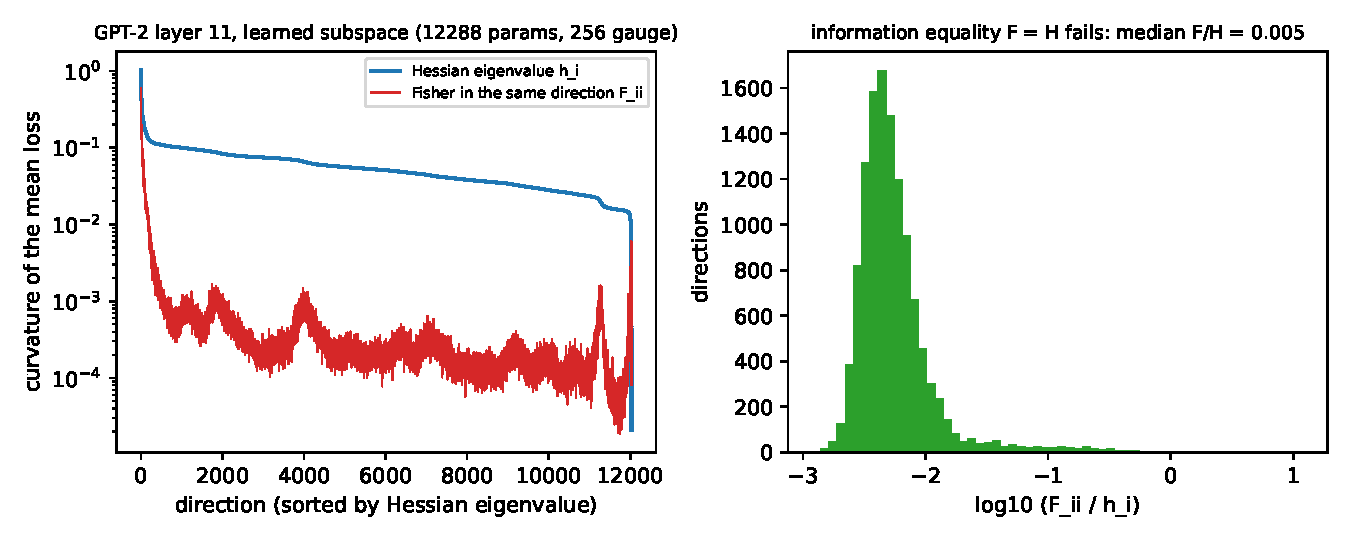
\includegraphics[width=\textwidth]{../talk_slt/gpt2_hessian_vs_fisher.pdf}
\caption{GPT-2 layer~11, learned $\dv=16$ subspace at its MAP on 1024 targets. Left: Hessian eigenvalues $h_i$ of the mean loss (12032 positive, 256 gauge zeros) and the empirical Fisher $F_{ii}$ in the same directions. Right: distribution of $\log_{10}(F_{ii}/h_i)$ over the curved directions, median $0.005$.}
\label{fig:gpt2fisher}
\end{figure}

\paragraph{Predicted and measured coefficients.} From the two matrices, a Laplace Bayes code of this family would pay $\tfrac12\sum_i nh_i/(nh_i+\alpha)=6016$ per $\ln n$ at every $n\ge1024$ (all directions resolved), i.e.\ about $65{,}000$ nats at $n=1024$, twenty times the label-only code; the plug-in's $\tfrac12\mathrm{tr}(FH^{-1})$ is $71$, of which 14 come from the top 100 directions and 24 from the top 1000. The measured coefficient of the MAP code, which on the subspace family is a maximum-likelihood single-map code (Section~\ref{sec:score:learners}) and so the plug-in code the formula describes, is $49\pm2$ on $n\le1024$ (Table~\ref{tab:gpt2ladder}), $45$ at 8192 and $37$ / $31$ / $19$ at 32768 on the three fit ranges (Section~\ref{sec:coef:scale}): the plug-in prediction is within a factor $1.5$ of the measurement, and the formula assumes the exact minimiser and the training-set Fisher. The second assumption was removed by recomputing the empirical Fisher on the 1000 i.i.d.\ evaluation targets at the same MAP: trace $14.0$ against $683$ ($2.0\%$), $F/H$ median $0.007$ and mean $0.012$ ($0.16$--$0.39$ in the top dozen), prediction $70.6$ against $71.2$ with the training-set Fisher. The mean gradient on fresh targets is $0.24$, so the fit does not generalise perfectly, but the second moment of the gradients is nearly the same: the generalisation Fisher of the subspace family is two per cent of its Hessian and the plug-in code's complexity is about 70, not 6016.

\paragraph{Mechanism.} The language model shares one mechanism with the oracle of Section~\ref{sec:coef:oracle}: the plug-in pays nothing in directions in which every example pushes the fit identically, so that the per-example gradients do not vary. On the oracle those directions are quartic, with $F=H=0$ in the population; on GPT-2 they are curved, but the information equality fails in almost every direction, $F$ being about one per cent of $H$. Moving the span in a typical direction changes the loss of every target in the same way, a deterministic cost, so the empirical minimiser has almost no sampling variance there and the plug-in pays nothing for those directions; the Bayes code must pay for the prior mass of the right 16-plane in a 12032-dimensional Grassmannian, which is astronomically small, while the plug-in finds the plane by gradient descent along directions that carry no noise. This is why the Laplace and Langevin codes of Sections~\ref{sec:bayescode} and~\ref{sec:learner} collapsed onto the prior and why no Bayes complexity charge ever appeared on the trained testbeds. The ordering of explanations under the plug-in code is correspondingly an ordering by Fisher-weighted curvature and not by nominal dimension: the coupling map with $1.9$~M parameters has $\kappa\approx170$--$225$ and the manufactured alignment $650$--$990$ (Section~\ref{sec:coef:scale}), because their Fisher is large in many more directions, every new base/source pair moving their fit.

\paragraph{Across loci and subspace dimensions.} The dense Hessian and the held-out empirical Fisher (on the 1000 i.i.d.\ targets, prior precision 0.01) were computed in the same way at layers 10 and 12 with $\dv=16$ and at layer~11 with $\dv=4$ and $\dv=64$, and the single-map MAP code was run at layer~11 with $\dv=4$ and $\dv=64$ (two seeds each, the protocol of the $\dv=16$ run). Table~\ref{tab:gpt2curv} sets the plug-in prediction $\tfrac12\mathrm{tr}(FH^{-1})$ against the measured plug-in coefficient $\kappa$ and against the nominal Bayes coefficient $\dv(d-\dv)/2$ of each family; Table~\ref{tab:gpt2dv} gives the measured coefficients of every configuration at the three widths. Three entries are pending: the eigendecomposition of the $49{,}152$-dimensional Hessian at $\dv=64$ and the MAP-code runs at layers 10 and 12 (job 1820081, running).

\begin{table}[t]
\centering
\footnotesize
\caption{GPT-2 IOI, valid subspace at its MAP on 1024 targets: Hessian spectrum, Fisher-to-Hessian ratio in the top dozen eigendirections (held-out Fisher), the plug-in prediction $\tfrac12\mathrm{tr}(FH^{-1})$, the measured plug-in coefficient $\kappa$ of the single-map MAP code (batching-corrected regret slope on $n=64$ to 1024; three seeds at $\dv=16$, two at $\dv=4$ and 64), and the nominal Bayes coefficient $\dv(d-\dv)/2$. ``Non-positive'' counts the gauge zeros ($\dv^2$) and, at layer~12, numerically negative eigenvalues.}
\label{tab:gpt2curv}
\resizebox{\textwidth}{!}{%
\begin{tabular}{lrrrcrrr}
\toprule
locus, $\dv$ & frame parameters & positive / non-positive & top $h$ & $F/H$, top dozen & predicted $\tfrac12\mathrm{tr}(FH^{-1})$ & measured $\kappa$ & nominal Bayes coefficient\\
\midrule
layer 10, 16 & 12{,}288 & 12{,}032 / 256 & 3.2 & 0.23--0.39 & 52.5 & pending & 6016\\
layer 11, 4 & 3072 & 3056 / 16 & 7.1 & 0.47--2.1 & 75.0 & $79.0\pm4.6$ & 1528\\
layer 11, 16 & 12{,}288 & 12{,}032 / 256 & 1.0 & 0.16--0.39 & 70.6 & $48.9\pm1.7$ & 6016\\
layer 11, 64 & 49{,}152 & pending & pending & pending & pending & $55.9\pm1.6$ & 22{,}528\\
layer 12, 16 & 12{,}288 & 11{,}328 / 960 & 24.2 & 0.29--0.78 & 111.7 & pending & 6016\\
\bottomrule
\end{tabular}}
\end{table}

\begin{table}[t]
\centering
\footnotesize
\caption{GPT-2 IOI, plug-in coefficients $\kappa$ of the single-map MAP code (batching-corrected regret slope per $\ln n$ on $n=64$ to 1024) at three subspace widths; three seeds at $\dv=16$ (Table~\ref{tab:gpt2ladder}), two at $\dv=4$ and 64. The coupling map interchanges the first $\dv$ of its coordinates. Last row: the MAP code's gain of the valid subspace over the label-only code (bits).}
\label{tab:gpt2dv}
\begin{tabular}{lrrr}
\toprule
configuration & $\dv=4$ & $\dv=16$ & $\dv=64$\\
\midrule
valid subspace, layer 11 & $79.0\pm4.6$ & $48.9\pm1.7$ & $55.9\pm1.6$\\
coupling map, layer 11 (trained network) & $389\pm12$ & $225.5\pm1.8$ & $160\pm3$\\
untrained twin, subspace, layer 11 & $26.7\pm0.3$ & $44.4\pm1.1$ & $48.4\pm2.4$\\
manufactured (coupling on the twin, layer 10) & $817\pm16$ & $988\pm93$ & $652\pm4$\\
coupling at layer 0 & $12.3\pm1.3$ & $12.3\pm0.9$ & $13.7\pm4.2$\\
\midrule
gain of the valid subspace over label-only & $+132$ (IIA 0.27) & $+3385$ & $+3499$\\
\bottomrule
\end{tabular}
\end{table}

The plug-in prediction is within a factor 1.1 of the measurement at $\dv=4$ (75 against 79) and within 1.45 at $\dv=16$ (71 against 49), the accuracy it has on the oracle. The measured coefficient of the valid subspace barely moves with the dimension of the family, 79, 49 and 56 at $\dv=4$, 16 and 64, while the nominal Bayes coefficient grows fifteenfold, from 1528 to 22{,}528. The plug-in pays for the Fisher-weighted directions, whose number is set by the data (how many name directions carry sampling noise), not by the parameter count. What the family's size does change is the loss term: a 4-plane cannot carry 16 names (IIA 0.27) and gains only 132 bits, while the 16- and 64-dimensional families gain 3385 and 3499 bits at almost the same coefficient. At layer~12, the state after the final normalisation, the loss is sharper (top eigenvalue 24 against 1) and 960 directions are numerically negative: the final normalisation makes the map's loss non-convex along the radial directions. The predicted coefficient there, 112, is the largest of the five; its measurement is pending. The controls scale the other way: the manufactured alignment's coefficient is 817, 988 and 652 and the trained coupling map's 389, 226 and 160 at $\dv=4$, 16 and 64, three to twenty times the valid subspace's at every width.

\paragraph{Confirmation: a genuine Bayes code of the InterpBench alignment is longer than label-only.} The HMC learner of Section~\ref{sec:coef:oracle} was run on InterpBench case~18 with the $\dv=4$ subspace map ($\mathcal N(0,1)$ prior on the frame, four chains of 100 samples after 200 warm-up iterations, 20 leapfrog steps), three seeds at 1024 targets and one seed at 8192 for the two subspace loci, with the regret measured against the MAP run's final fit on the same targets. Unlike on the oracle, the chains do \emph{not} continue across blocks here: at every block the learner starts fresh chains from draws of the prior, moves them by 200 Adam steps on the energy, resets the step size, and then runs the 200 warm-up iterations and draws the 100 samples per chain. (An earlier version of this analysis stated that the chains continued across blocks; the runner restarts them.) Each block's posterior sample therefore comes from chains that have run only that block's warm-up.

Table~\ref{tab:ibhmc} gives the codes. At 1024 targets the Bayes code of the \emph{valid} alignment is $1526$, $2370$ and $1898$ bits on the three seeds, longer than the label-only code of $1342$ bits, where the plug-in codes gain about a thousand bits ($+983\pm11$ under the mixture, $+1051.5\pm33.8$ under the MAP code), and its regret against the plug-in's final fit grows at $269\pm43$ per $\ln n$ against the plug-in's $8\pm3$ (Table~\ref{tab:ha3ib}). The misspecified locus codes $1935$--$2158$ bits at the same slope ($271\pm10$); the wrong locus \texttt{resid\_0} gains nothing ($2531$--$2620$ bits, slope $-6$ to $-8$); the untrained twin's $1633$ bits on every seed is the prior predictive, the chains never leaving the prior because there is nothing to learn. HMC acceptance is $0.52$--$0.82$ throughout, and the final IIA of the sampled predictive is $0.98$ on two valid seeds and $0.48$ on the third: the posterior has not concentrated by $n=1024$. At 8192 targets it has (IIA $1.00$, $3707$ bits against a label-only code of about $10{,}700$), and the valid Bayes code still trails the plug-in's by about $1175$ nats, with the misspecified locus at $10{,}530$ bits. This is what the Hessian and Fisher analysis predicts: the subspace family is regular on its 1024-dimensional Grassmannian, a Bayes code pays for the prior mass of the right 4-plane, of order $\lambda\ln n$ with $\lambda$ up to 512, and the plug-in finds the plane along Fisher-free directions at no charge.

\begin{table}[t]
\centering
\footnotesize
\caption{InterpBench case~18, $\dv=4$ subspace family: the Bayes code by HMC (bits on the coded targets, per seed at 1024 targets; label-only 1342 bits) and its batching-corrected regret slope against the MAP run's final fit, next to the single-map MAP code's gain over label-only and slope from Sections~\ref{sec:results} and~\ref{sec:ha3ib:ib}. The HMC chains restart at every block.}
\label{tab:ibhmc}
\resizebox{\textwidth}{!}{%
\begin{tabular}{llrr}
\toprule
configuration & Bayes code (bits, 3 seeds) & slope vs.\ MAP reference & MAP code: gain / slope \\
\midrule
valid subspace at \texttt{resid\_2} & 1526 / 2370 / 1898 & $269\pm43$ & $+1051.5\pm33.8$ / $8\pm3$ \\
misspecified subspace at \texttt{resid\_1} & 1935 / 1949 / 2158 & $271\pm10$ & slope $\approx107$ \\
wrong locus \texttt{resid\_0} & 2531--2620 & $-6$ to $-8$ & \\
untrained twin (\texttt{resid\_1}, \texttt{resid\_2}) & 1633 (all seeds) & 6 & \\
coupling at \texttt{resid\_2} (trained) & 1802 / 1837 & 236 & slope 474 \\
manufactured (coupling on the twin) & 2045 (1 seed) & 263 & slope 255 \\
\midrule
8192 targets, valid (1 seed) & 3707 (IIA 1.00) & 161 / 107 ($n\ge64$ / $\ge512$) & \\
8192 targets, misspecified (1 seed) & 10530 & 746 / 1173 & \\
\bottomrule
\end{tabular}}
\end{table}

\subsection{Where the Bayes code is the right instrument: hierarchical equality, and a ladder in $n$ against $\lambda$}
\label{sec:coef:ladder}

\paragraph{Run.} The HMC learner was run on hierarchical equality (Section~\ref{sec:tb:heq}) with the rotation family: the configurations of Table~\ref{tab:toy} except the second twin, five seeds, the same 1024 targets and label-only code (1021.1 bits), an $\mathcal N(0,1)$ prior on the map parameters, four chains of 100 samples after 200 warm-up iterations, 20 leapfrog steps and initial step $0.01$. As on InterpBench the chains restart at every block. The rotation at a hidden layer of width 32 with $\dv=4$ has 496 parameters and the nominal coefficient $\dv(d-\dv)/2=4\cdot28/2=56$. The gauge defect of Section~\ref{sec:gauge} concerns the Laplace Gaussian at the mode, whose Hessian does not follow the curved fibres of $\exp(S)$; HMC samples the posterior itself, so this is a genuine Bayes code of the rotation family, under the pushforward of the $\mathcal N(0,1)$ prior on the skew entries, which is not the uniform distribution on the Grassmannian. The nominal coefficient 56 is the Grassmannian's; the rotation family shares it wherever the map from $S$ to the span of the first $\dv$ columns of $\exp(S)$ is a submersion, which holds almost everywhere, but its prior, and with it the $O_p(1)$ terms of~\eqref{eq:watanabe}, differ. The regret slopes are taken against the sampled predictive's own final fit, so they estimate the Bayes coefficient, here in the interpolation regime ($n\le1024$ against 496 parameters). Table~\ref{tab:toyhmc} sets the Bayes code against the canonical mixture of four of Table~\ref{tab:toy}.

\begin{table}[t]
\centering
\footnotesize
\caption{Hierarchical equality, $\dv=4$ rotation family: the Bayes code by HMC against the plug-in mixture of four (Table~\ref{tab:toy}), five seeds, same targets. Gains over the label-only code (1021.1 bits), mean $\pm$ s.e., i.i.d.\ IIA in brackets. Lower block: gains of the valid alignment against its controls, the Bayes code's regret slopes per $\ln n$ against its own final fit ($n\ge64$), and the competence-onset trajectory.}
\label{tab:toyhmc}
\resizebox{\textwidth}{!}{%
\begin{tabular}{lll}
\toprule
configuration & Bayes code (HMC) & plug-in (mixture of four)\\
\midrule
valid: $h_1$ rotation & $+733.0\pm0.8$ (1.00) & $+505.5\pm19.3$ (1.0)\\
misspecified: $h_2$ rotation & $+80.7\pm43.1$ (0.68) & $-404.9\pm2.2$ (0.7)\\
wrong locus (input) & $-76.3\pm47.5$ (0.72) & $-745.5\pm32.7$ (0.6)\\
untrained twin at $h_1$ / $h_2$ & $-13.8$ / $-14.2$ (0.5) & $-9.1$ / $-13.9$ (0.5)\\
coupling at $h_1$, trained network & $-322.2\pm36.0$ (0.5) & $+586.5\pm6.2$ (1.0)\\
manufactured (coupling on the twin, $h_2$) & $-380.9\pm34.6$ (0.5) & $-570.9\pm19.8$ (0.5)\\
\midrule
valid vs.\ twin / coupling / wrong locus & $+747\pm1$ / $+1055\pm35$ / $+809\pm47$ & $+514.6$ / $-81.0$ / $+1251.0$\\
regret slope: valid / coupling / wrong locus / twin & $12.9\pm0.1$ / $22.8\pm7.7$ / $58.5\pm15.3$ / $0.17$ & \\
valid $h_1$ at checkpoints 128 / 256 / 1024 & $+184$ / $+697$ / $+730$ & $+227$ / $+644$ / $+580$\\
\bottomrule
\end{tabular}}
\end{table}

\paragraph{Here the Bayes code is the shorter one.} The Bayes code of the valid alignment gains $+733.0\pm0.8$ bits over label-only, about 230 bits more than the plug-in mixture. The posterior predictive hedges where the plug-in maps overfit the early blocks, and the complexity it must pay (regret 88 nats at $n=1024$, slope $12.9\pm0.1$, a quarter of the nominal 56) is small against the loss gain on 1000 targets. All five seeds reject the twin, the coupling map and the wrong locus at $\alpha=0.01$ by $n=35$--75.

\paragraph{The Bayes code charges the other family; the plug-in does not.} The coupling family at $h_1$ gains $+586.5$ bits as a plug-in and loses $322.2\pm36.0$ bits as a Bayes code: the prior mass of the faithful coupling maps is tiny, the posterior has not concentrated after 1024 targets, and the predictive stays near the prior (IIA 0.5). Under the plug-in the coupling map codes 81 bits shorter than the valid rotation (Section~\ref{sec:res:heq}); under the Bayes code the rotation is 1055 bits ahead. The Bayes code orders the two families by their Bayes coefficients, the ordering the learning-coefficient hypothesis describes. The misspecified locus $h_2$ moves from $-405$ (plug-in) to $+81$ bits: the hedged predictive is better than label-only on the 68\% of targets it gets right and does not pay the plug-in's overconfident losses. Along training the Bayes gain does not fall back after competence onset ($+697$ at step 256, $+730$ at step 1024), where the plug-in's does ($+644$, $+580$).

\begin{table}[t]
\centering
\footnotesize
\caption{The ladder in $n$ against $\lambda$: the valid alignment's Bayes code and plug-in code at 1024 targets on three testbeds of increasing width. Bayes regret slopes are against the sampled predictive's own final fit on hierarchical equality and against the MAP run's final fit on InterpBench; on GPT-2 the Bayes coefficient is the Laplace count of Section~\ref{sec:coef:gpt2} and the Bayes code was not run.}
\label{tab:ladder}
\setlength{\tabcolsep}{4pt}
\begin{tabular}{llll}
\toprule
 & hierarchical equality & InterpBench case~18 & GPT-2 IOI, layer 11\\
\midrule
locus width $d$, $\dv$ & 32, 4 & 260, 4 & 768, 16\\
nominal Bayes coefficient & 56 & 512 & 6016\\
Bayes code at 1024 targets & $+733.0\pm0.8$ bits & 1526 / 2370 / 1898 bits & not run\\
 & & (label-only 1342) & (about $65{,}000$ nats predicted)\\
Bayes regret slope & $12.9\pm0.1$ & $269\pm43$ & 6016 (Laplace count)\\
plug-in code at 1024 targets & $+505.5\pm19.3$ (mixture) & $+1051.5\pm33.8$ (MAP) & $+3384.6\pm4.9$ (MAP)\\
plug-in $\kappa$ & -- & $8.4\pm2.9$ & $48.9\pm1.7$\\
\bottomrule
\end{tabular}
\end{table}

\paragraph{The ladder.} Together with InterpBench case~18 (Table~\ref{tab:ibhmc}) and GPT-2 (Section~\ref{sec:coef:gpt2}), the three testbeds form a ladder in $n$ against $\lambda$ (Table~\ref{tab:ladder}). At a nominal coefficient of 56 the Bayes code is shorter than the plug-in and charges the expressive family. At 512 it is longer than the label-only code at 1024 targets and concentrates only by 8192, where it still trails the plug-in by about 1175 nats. At 6016 it would cost about $65{,}000$ nats at 1024 targets, twenty times the label-only code. The Bayes code is the right instrument when $\lambda\ln n$ is small against the loss gain, uncompetitive when $\lambda$ is a few hundred at $n=1024$, and unusable at thousands. The plug-in's coefficient $\tfrac12\mathrm{tr}(FH^{-1})$ stays at tens on every rung, which is why the plug-in is the operative code of this paper.

\subsection{Scale dependence of the plug-in's coefficient}
\label{sec:coef:scale}

\paragraph{Learner coefficients at 1024 targets.} Table~\ref{tab:gpt2ladder} collects the regret slopes of the single-map MAP code for every recorded configuration on GPT-2 and InterpBench at $n\le1024$, the numbers behind the complexity ladder of Section~\ref{sec:jlens}. The manufactured alignment's coefficient is twenty times the valid alignment's on GPT-2 ($988$ against $49$) and thirty times on InterpBench ($255$ against $8$): the expressive map on the untrained network keeps paying for every block, the valid subspace stops paying once its span is found. The same coupling family on the \emph{trained} network has a coefficient of $225$ (GPT-2) and $474$ (InterpBench), so the family's coefficient depends on the network it is attached to, i.e.\ on the data distribution, as a learning coefficient should. The Langevin-hedged arm of Section~\ref{sec:learner} reproduces every GPT-2 slope within 2 nats. Both valid subspaces were measured below their parameter count here (12288 and 1040 frame parameters at $n\le1024$); the larger runs follow.

\begin{table}[t]
\centering
\footnotesize
\caption{Learner coefficients of the single-map MAP code (batching-corrected regret slope per $\ln n$ on $n=64$ to 1024, three seeds) and regret at $n=1024$ for every recorded configuration. GPT-2: width 768, $\dv=16$, nominal Grassmannian $\lambda=6016$, 12288 frame parameters, coupling map $1.9$~M parameters. InterpBench case~18, variable \texttt{freq}, $\dv=4$: width 260, nominal $\lambda=512$, 1040 frame parameters.}
\label{tab:gpt2ladder}
\resizebox{\textwidth}{!}{%
\begin{tabular}{llrrl}
\toprule
testbed & configuration & slope & regret at 1024 (nats) & note \\
\midrule
GPT-2 & valid subspace, layer 11 & $48.9\pm1.7$ & 279 & $n<$ frame parameters \\
GPT-2 & coupling map at layer 11 (trained network) & $225.5\pm1.8$ & 1102 & \\
GPT-2 & untrained twin, subspace, layer 11 & $44.4\pm1.1$ & 205 & learns the twin's name copy \\
GPT-2 & manufactured alignment (coupling, twin 7, layer 10) & $988\pm93$ & 4323 & IIA 0.86 on the training names \\
GPT-2 & manufactured alignment (coupling, twin 8, layer 10) & $950\pm82$ & 4174 & \\
GPT-2 & layer 0, subspace (trained or twin) & $0.0$ & 0 & predictor identical in every block \\
GPT-2 & layer 0, coupling & $12.3\pm0.9$ & 89 & \\
\midrule
InterpBench & valid subspace at \texttt{resid\_2} & $8.4\pm2.9$ & 49 & interpolation regime \\
InterpBench & coupling at \texttt{resid\_2} (trained network) & $474\pm1$ & 2114 & \\
InterpBench & manufactured alignment (coupling, twin, \texttt{resid\_2}) & $255\pm130$ & 1108 & \\
InterpBench & misspecified subspace at \texttt{resid\_1} & $107\pm15$ & 529 & excess-loss drift \\
InterpBench & wrong locus \texttt{resid\_0} & $109\pm10$ & 494 & \\
\bottomrule
\end{tabular}}
\end{table}

\paragraph{InterpBench to 32768 targets.} The 32768-target MAP runs on case~18 are reported in Section~\ref{sec:ha3concl} (Table~\ref{tab:ha3ib32768}). The valid alignment's coefficient keeps rising slowly with the fit range, $22.6\pm4.1$, $27.1\pm5.7$, $31.7\pm8.4$ on $n\ge64$, $\ge512$, $\ge2048$ at $\dv=4$ and $32.6\pm2.0$, $40.5\pm0.1$, $42.0\pm0.0$ at $\dv=1$, so the plug-in coefficient of the 1040-parameter subspace family on InterpBench is roughly 30--40 on $n\in[2048,32768]$, 6--8\% of the nominal 512. The misspecified locus is four to six times higher ($120$--$186$). The caveat specific to InterpBench is the interpolation regime: below the frame's 1040 parameters the fits interpolate and the regret is flat (Figure~\ref{fig:ibregret}), so the coefficient can only be read beyond $n\approx2000$, and whether it settles is still open at this range.

\begin{figure}[htbp]
\centering
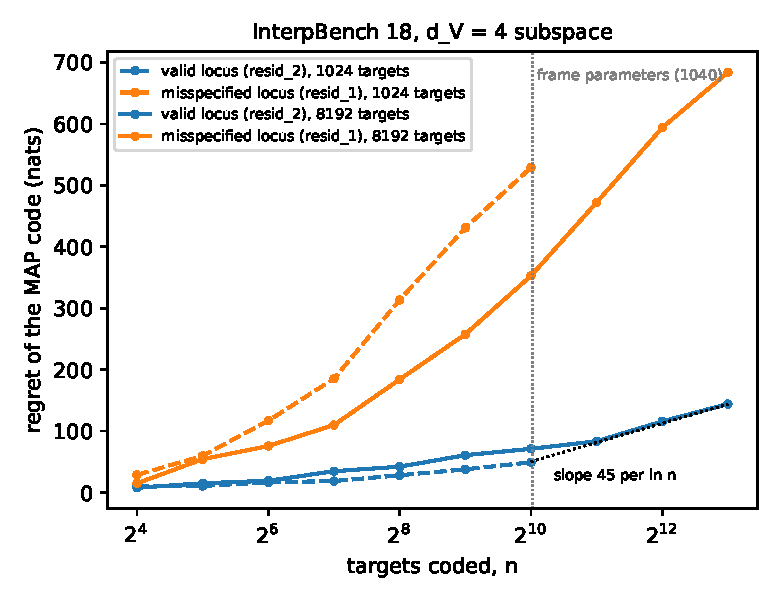
\includegraphics[width=0.8\textwidth]{../talk_slt/interpbench_regret_vs_n.pdf}
\caption{InterpBench case~18, $\dv=4$ subspace, regret of the MAP code at the valid and the misspecified locus, 1024- and 8192-target runs (Tables~\ref{tab:ha3ib} and~\ref{tab:ha3ib8192}). The regret is flat below the frame's 1040 parameters and grows at about 45 per $\ln n$ beyond; the misspecified locus grows from the excess-loss drift.}
\label{fig:ibregret}
\end{figure}

\paragraph{GPT-2 to 32768 targets.} The single-map MAP code on GPT-2 IOI (Sections~\ref{sec:score:learners} and~\ref{sec:learner}; layers 0 and 11, the adversary at layer~10) was run with 8192 and 32768 targets on one seed, and the 32768-target run was repeated on two further seeds. Table~\ref{tab:gpt2largen} gives the batching-corrected slopes on several fit ranges, and Figure~\ref{fig:gpt2regret} the regret curves. The valid subspace's coefficient is stable at roughly 45--50 per $\ln n$ from $n=32$ to $16384$ on the one-seed run (block-end regrets $21$, $35$, $75$, $109$, $147$, $172$, $224$, $278$, $312$, $358$, $389$, $365$ nats; local slopes $20$, $57$, $50$, $54$, $37$, $75$, $77$, $50$, $66$, $46$, $-36$), i.e.\ about 100 constrained directions of the 12288-parameter frame, and on three seeds $41.6\pm5.0$, $40.9\pm9.2$ and $34.6\pm14.6$ on $n\ge64$, $\ge1024$ and $\ge4096$ with $419$ nats at 32768. There is no interpolation plateau on GPT-2, unlike InterpBench, although $n$ crosses the parameter count only at 12288: the regret grows at the same rate below and above it. The negative last step is the final fit on 32768 targets being slightly worse than the block predictor (400 Adam steps from a cold start on minibatches of 256 of the 32768 pairs), a limitation of the best-in-family proxy and not of the code.

The manufactured alignment pays $6775$ nats by 32768 targets on the one-seed run and $7081$ on three seeds, 17--19 times the valid alignment; its local coefficient peaks at $1700$--$2450$ between $n=512$ and 2048, where new base/source combinations expose what the expressive map memorised, and settles near $600$--$1300$ afterwards (block-end regrets $38$, $130$, $290$, $488$, $1066$, $2242$, $3943$, $4374$, $4896$, $5605$, $6526$, $6775$). The same coupling family on the trained network pays $165$--$195$ per $\ln n$ on the one seed and $129$--$146$ on three; the untrained twin's own subspace code grows faster at large $n$ ($41$ to $66$), the twin's copy of the name tokens being read out progressively. The coupling at layer~0, where the subspace map learns nothing (slope 0 at every $n$), grows from $12$ to $152$ with the fit range.

\begin{table}[t]
\centering
\footnotesize
\caption{GPT-2 IOI, single-map MAP code: batching-corrected regret slopes per $\ln n$ of every configuration at 1024 targets (three seeds), 8192 targets (one seed, $n\ge64$) and 32768 targets (one seed, three fit ranges; then three seeds), and the seed-mean regret at 32768. Layer~0 with the subspace map has slope 0 at every $n$ (the predictor is identical in every block).}
\label{tab:gpt2largen}
\resizebox{\textwidth}{!}{%
\begin{tabular}{lrrrrrr}
\toprule
configuration & $n{=}1024$ & 8192 & 32768, $n\ge64$ & $n\ge1024$ & $n\ge4096$ & regret at 32768 \\
\midrule
valid subspace, layer 11 & $48.9\pm1.7$ & $44.6\pm7.9$ & $37.0\pm3.3$ & $30.9\pm8.6$ & $19\pm17$ & 365 \\
\quad three seeds & & & $41.6\pm5.0$ & $40.9\pm9.2$ & $34.6\pm14.6$ & 419 \\
coupling map, layer 11 (trained) & $225.5\pm1.8$ & $195.1\pm7.2$ & $174.8\pm8.7$ & $163\pm11$ & $167\pm15$ & 1803 \\
\quad three seeds & & & $146\pm18$ & $131\pm29$ & $129\pm40$ & 1523 \\
untrained twin, subspace, layer 11 & $44.4\pm1.1$ & $41.4\pm3.6$ & $41.1\pm4.1$ & $52.8\pm8.0$ & $66\pm13$ & 442 \\
manufactured (coupling on the twin, layer 10) & $988\pm93$ & $912\pm87$ & $798\pm66$ & $609\pm60$ & $656\pm138$ & 6775 \\
\quad three seeds & & & $826\pm35$ & $726\pm63$ & $795\pm70$ & 7081 \\
coupling at layer 0 & $12.3\pm0.9$ & $7.0$ & $48.5$ & $95.6$ & $152$ & 530 \\
\bottomrule
\end{tabular}}
\end{table}

\begin{figure}[htbp]
\centering
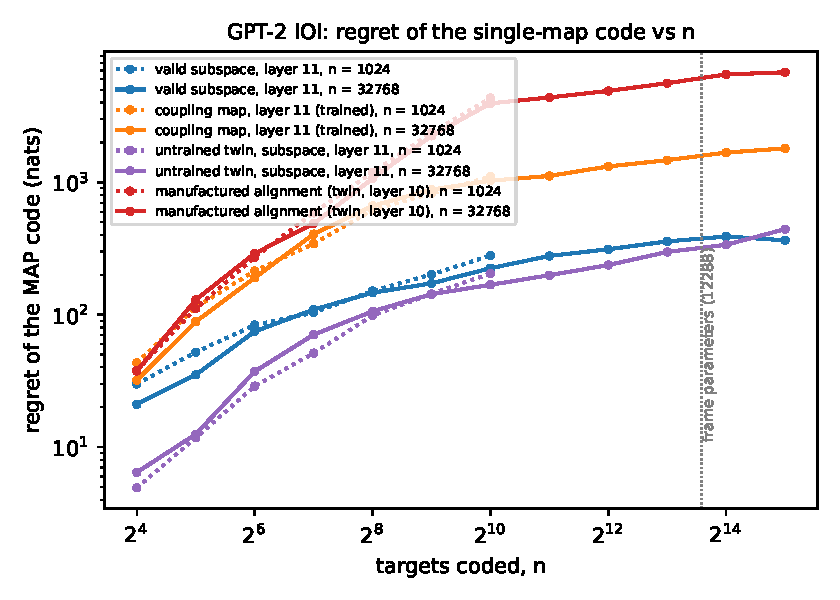
\includegraphics[width=0.8\textwidth]{../talk_slt/gpt2_regret_vs_n.pdf}
\caption{GPT-2 IOI, regret of the single-map MAP code against $n$ for the valid subspace, the coupling map on the trained network, the untrained twin's subspace and the manufactured alignment, 1024- and 32768-target runs (Table~\ref{tab:gpt2largen}). No interpolation plateau at the frame's 12288 parameters.}
\label{fig:gpt2regret}
\end{figure}

\subsection{Consequences}
\label{sec:coef:consequences}

\begin{enumerate}
\item \emph{The plug-in's $\kappa$ is the operative complexity of an explanation.} The score of this paper is a plug-in (or mixture-of-plug-ins) code, and its regret slope is $\tfrac12\mathrm{tr}(FH^{-1})$ up to the approximations noted: a count of the directions in which the data move the fit, weighted by how much. On GPT-2 this is about 70 predicted and 45--50 measured for the valid subspace, $130$--$225$ for the coupling map on the trained network and $600$--$990$ for the manufactured alignment, against a nominal $\lambda$ of 6016 for the subspace family alone. It does not grow with the family: 79, 49 and 56 at $\dv=4$, 16 and 64 against nominal Bayes coefficients from 1528 to 22{,}528 (Table~\ref{tab:gpt2curv}). The ordering of explanations the code produces is an ordering by this quantity, and it is the ordering that separates valid from manufactured alignments by a factor of 20 on GPT-2 and 30 on InterpBench (Table~\ref{tab:gpt2ladder}).
\item \emph{At the widths of InterpBench and GPT-2 the Bayes learning coefficient of an alignment family is real, large, and not what makes explanations short.} On reduced-rank regression the Bayes code's slope is Aoyagi--Watanabe's $\lambda$ exactly; on the oracle it is measurable by HMC and differs from the MAP code's in both directions; on GPT-2 it is 6016 by the Laplace count, and on InterpBench the genuine Bayes code of the valid alignment is longer than the label-only code at 1024 targets. A Bayes code of an alignment family attached to a trained network pays for prior mass on a Grassmannian along directions that carry no noise, and that payment does not distinguish a valid alignment from a manufactured one in the direction the preregistered evaluation needs (Table~\ref{tab:ibhmc}: the valid, the misspecified, the coupling and the manufactured codes all have slopes $236$--$271$ against the plug-in reference). The question raised by the layer-10 adversary in Section~\ref{sec:adversary}, whether a Bayes or Laplace code for the map family restores the absolute form of the rejection criterion, is therefore answered in the negative for the right reason: not because the chains were too short (Section~\ref{sec:learner}) but because the quantity such a code would charge is the wrong one. Hierarchical equality marks the limit of this statement: there the nominal coefficient is 56, $\lambda\ln n$ is small against the loss gain, the Bayes code of the valid alignment is about 230 bits shorter than the plug-in's, and it turns the coupling family's $+586.5$ bits under the plug-in into $-322.2$ (Section~\ref{sec:coef:ladder}).
\item \emph{The ``effective coefficient'' of Section~\ref{sec:ha3eff} is the plug-in code's.} The statement that the law holds with $\lambda_{\mathrm{eff}}=\dv k/2$, half the readable directions, was verified with the MAP code (Table~\ref{tab:ksweep}: slopes $0.53$ to $4.49$ for $k/2$ from $0.5$ to $5.5$) and is correct for it, as $\tfrac12\mathrm{tr}(FH^{+})$ confirms; the Bayes coefficient of the same family on the same oracle is $k/2+(11-k)/4$, from $3.0$ to $5.5$, which counts the unreadable directions as quartic at $1/4$ each; the Bayes code's slopes reach it with 16384 targets ($3.05$ to $5.43$) after $1.98$ to $4.72$ on $n\le2048$ (Table~\ref{tab:oracle16384}). The three regimes of Section~\ref{sec:ha3concl} are likewise regimes of the MAP code: in the sharp-readout regime the Bayes coefficient itself rises from $k/2$ to $k$ on $n\le2048$ and falls back to $3.55$ with 16384 targets, while the MAP's $14.2$ is a learner excess over it that stays at $10.3$. The measured numbers of Sections~\ref{sec:ha3eff}--\ref{sec:ha3concl} stand; the words ``learning coefficient'' and ``$\lambda_{\mathrm{eff}}$'' there are to be read as the learner coefficient $\kappa$ of the plug-in code, which revises the reading under which those sections were first written.
\item \emph{The LLC sampler and the regret slope estimate different things on the trained testbeds.} On reduced-rank regression the Langevin LLC reads $\lambda$ (Section~\ref{sec:coef:rrr}). On the oracle it reads $0.85$ to $4.20$ (Section~\ref{sec:ha3concl}; Figure~\ref{fig:oracleeff}), close to $k/2$ and to the MAP code's slope, and below the Bayes learning coefficient $k/2+(11-k)/4$ at every $k$ ($3.0$ at $k=1$, where the Bayes code's slope is $1.98\pm0.26$ on $n\le2048$ and $3.35\pm0.50$ on $n\le16384$); only at $k=11$ do the LLC, the MAP code's slope and the Bayes code's slope on $n\le2048$ nearly coincide ($4.20$, $4.49$ and $4.72$). An earlier version of this item stated that the LLC reads $\lambda$ on the oracle as well, which predates the Bayes code by HMC and holds only where $\kappa$ and $\lambda$ are close. On InterpBench the sampler fails for its own reason (Section~\ref{sec:ha3concl}: no plateau, the chains measure the extent of the flat region), and even a converged sampler would return a Bayes quantity of order hundreds, not the plug-in's 8--45. The regret slope of the code is therefore not an LLC estimator on trained networks, and is not reported as one.
\end{enumerate}

\section{The Jacobian lens: the parameter-free floor of the complexity ladder}
\label{sec:jlens}

\paragraph{Construction.} The Jacobian lens of Gurnee et al.\ \cite{gurnee2026workspace} reads a mid-layer state through the network's own averaged Jacobian.\footnote{The Jacobian lens was introduced to study which content of a mid-layer state of a language model is \emph{verbalizable}, i.e.\ expressed as output tokens later in the computation; its originators call it an imperfect tool \cite{gurnee2026workspace}.} Its coordinate swap is a distributed interchange intervention whose subspace is given analytically rather than learned, so it is an alignment family with no fitted parameters, and we add it to the comparison as the floor of the complexity ladder. For a layer $\ell$ let $J_\ell$ be the Jacobian of the final-layer state with respect to the layer-$\ell$ state, averaged over prompts and positions, and $v_w=(W_UJ_\ell)_w$ the J-vector of token $w$, where $W_U$ is the unembedding matrix: the average direction at layer $\ell$ that makes $w$ more likely later. For a variable with token values $w_1,\dots,w_m$, let $V_J$ have the unit-normalised $v_{w_j}$ as columns and $Q$ be an orthonormal basis of the complement of their span; the J-lens alignment is the linear bijection $\phi_J(h)=(V_J^{+}h,\,Q^{\!\top}h)$, whose interchange intervention transplants the J-coordinates of the source into the base and leaves the base's complement untouched. Its distortion is $\mathrm{cond}(V_J)$, a property of the network alone, and the interchange itself is an isometry.

The averaged Jacobian also splits the sensitivity of an intervention pair into a predicted part and a residual. The \emph{Jacobian consistency} $\mathrm{JC}=\|\delta-W_UJ_\ell\Delta\|/\|\delta\|$, with $\Delta$ the difference of two intervened states (one base with two sources) and $\delta$ the actual logit difference, is small when the intervention acts through the directions the downstream computation uses on average and large when it relies on local sensitivity the average does not show, which is what a manufactured alignment paying through off-manifold sensitivity must do.

\paragraph{Hypothesis.} The Jacobian-lens hypothesis of our research plan makes three claims: on token-valued variables the J-lens reaches an IIA within the margin of the best rotation at loci where the value is verbalizable, at zero parametric cost, with $\mathrm{cond}(V_J)$ below a small constant; on untrained networks it fails for copied variables such as the indirect-object name, where learned reversible maps succeed, because it has no freedom to route; and manufactured alignments that pass held-out IIA show Jacobian consistency well above that of valid ones on the same pairs.

\paragraph{Run.} On GPT-2 IOI (Section~\ref{sec:tb:ioi}) the J-vectors were taken as the gradient of each name's final logit (among the 32 name logits) with respect to the residual state at the locus at the final position, averaged in double precision over the first 1000 prompts of the pool, all of which use training names. At layer~12, the state after the final layer normalisation, only the unembedding follows, so the J-vectors there are the unembedding rows of the names and the lens reduces to the logit lens.\footnote{The \emph{logit lens} reads an intermediate state by applying the network's final unembedding to it directly, as if the remaining layers were absent.} The frame is the span of the unit J-vectors (their left singular vectors with singular value above $10^{-6}$ times the top one), completed to an orthonormal basis, in two variants: ``all'', the 32 names of the output alphabet (rank 32), and ``train'', the 16 training names (rank 16), the latter being the fair comparison with the learned maps, which see only the training names. Since nothing is fitted, the prequential code is one predictor's loss on every target and the learner coefficient is exactly 0. The targets and the label-only code ($4324.5$ bits) are those of every GPT-2 run of this paper. The Jacobian consistency is computed on 500 triples (a base with two sources) from the i.i.d.\ evaluation split, for the J-lens, for a single learned subspace map ($\dv=16$, 400 Adam steps, learning rate $10^{-2}$, fitted on all 1024 targets) on the trained network, and for a coupling map (4 blocks of width 512, 4000 steps, learning rate $10^{-3}$) on the untrained twin, whose consistency is computed with the twin's own averaged Jacobian. Table~\ref{tab:jlens} gives the run. Its layer-0 row is corrected from an earlier version of this table, which repeated the layer-9 code (7591 bits, $-3267$) from the report file; the stored record gives 7842 bits ($-3518$, $\mathrm{cond}(V_J)=420$). The layer-6 gain, earlier given as about $-3200$ bits, is $-3520$, and the twin's condition numbers span 1.3--2.4 rather than 1.3--1.5 once layers 0 and 6 are included.

\begin{table}[t]
\centering
\footnotesize
\caption{The Jacobian-lens alignment on GPT-2 IOI (variable \texttt{io}): condition number of $V_J$, code in bits on the 1016 coded targets, gain over the label-only code (4324.5 bits), and IIA on the i.i.d.\ and disjoint-name splits. Learned maps on the same targets for comparison. Lower block: Jacobian consistency (median / mean / 90th percentile over 500 triples from the i.i.d.\ split); the manufactured alignment's consistency is computed on the twin's own averaged Jacobian. The layer-6 row, omitted, also fails (IIA 0.07, gain $-3520$ bits, $\mathrm{cond}(V_J)=162$).}
\label{tab:jlens}
\begin{tabular}{lllrrrcc}
\toprule
network & names & locus & $\mathrm{cond}(V_J)$ & code & gain over label-only & IIA iid & IIA shifted \\
\midrule
trained & all & layer 0 & 420 & 7842 & $-3518$ & 0.07 & 0.06 \\
trained & all & layer 9 & 121 & 7592 & $-3267$ & 0.07 & 0.06 \\
trained & all & layer 10 & 119 & 1504 & $+2821$ & 0.80 & 0.78 \\
trained & train & layer 10 & 75 & 1530 & $+2794$ & 0.78 & 0.06 \\
trained & all & layer 11 & 111 & 795 & $+3529$ & 0.98 & 0.99 \\
trained & train & layer 11 & 68 & 800 & $+3525$ & 0.98 & 0.07 \\
trained & all & layer 12 & 7.6 & 698 & $+3626$ & 1.00 & 0.99 \\
trained & train & layer 12 & 4.6 & 707 & $+3618$ & 1.00 & 0.07 \\
untrained twin & any & any & 1.3--2.4 & 5169--5180 & $-845$ to $-855$ & 0.04 & 0.00 \\
\midrule
\multicolumn{8}{l}{\emph{learned maps, gain over label-only}:}\\
\multicolumn{8}{l}{\quad subspace $\dv=16$ at layer 11 $+3302\pm3$ (mixture, 5 seeds), $+3385\pm5$ (MAP, 3 seeds);}\\
\multicolumn{8}{l}{\quad layer 10 $+2975$, layer 12 $+3145$ (mixture); coupling at layer 11, trained, $+2459\pm16$ (MAP);}\\
\multicolumn{8}{l}{\quad manufactured, layer 10, $+704\pm63$ (mixture), $-1985\pm602$ (MAP)}\\
\midrule
\multicolumn{8}{l}{\emph{Jacobian consistency}, layer 10: J-lens $0.26$ / $0.37$ / $0.82$ (IIA 0.80); learned subspace $0.38$ / $0.49$ / $0.93$ (0.97);}\\
\multicolumn{8}{l}{\quad manufactured $2.05$ / $2.58$ / $4.84$ (0.80)}\\
\multicolumn{8}{l}{layer 11: J-lens $0.15$ / $0.21$ / $0.42$ (0.98); learned subspace $0.24$ / $0.29$ / $0.56$ (0.99);}\\
\multicolumn{8}{l}{\quad manufactured $2.24$ / $2.48$ / $4.04$ (0.84)}\\
\bottomrule
\end{tabular}
\end{table}

\paragraph{The hypothesis holds on all three claims.} At the loci where the name is verbalizable the parameter-free alignment is as faithful as the learned subspace, IIA $0.98$ at layer~11 and $1.00$ at layer~12, and its code is \emph{shorter}: $+3529$ and $+3626$ bits over label-only (``all''; $+3525$ and $+3618$ with the 16 training names) against $+3302$ and $+3145$ for the learned subspace under the mixture code and $+3385$ for the single MAP map at layer~11. At layer~10 the learned map wins ($+2975$ against $+2821$; IIA $0.97$ against $0.80$), and at layer~9 and below the lens fails (IIA $0.07$, chance for 16 names), where the learned subspace also fails. On the untrained twin it fails everywhere (IIA $0.04$, code about 850 bits longer than label-only), as predicted for a copied variable the twin cannot route. And the Jacobian-consistency statistic separates the manufactured alignment from both valid ones by a factor of six to ten at the median, $2.0$--$2.2$ against $0.15$--$0.38$: the manufactured map moves the output through local sensitivity that the network's averaged Jacobian does not show. The hypothesis also asks that $\mathrm{cond}(V_J)$ stay below a small constant: the measured distortion of $\phi_J$ is $68$--$121$ at layers 9--11 on the trained network, $4.6$--$7.6$ at the final locus and $1.3$--$2.4$ on the twin, which we record without reading it against that clause, since the hypothesis does not fix the constant; the interchange itself is an isometry.

\paragraph{Fairness of the name frames.} The ``all'' variant generalises to the 16 unseen names (shifted IIA $0.99$) because their directions are in its frame; the ``train'' variant, which sees only what the learned maps see, matches the learned map's failure on unseen names ($0.07$). Generalisation across names is a property of which directions are in the frame, not of learning, and the disjoint-name failure discussed in Section~\ref{sec:limits} is to be read with this in mind: the 16-name lens and the 16-name learned subspace fail alike, and the comparison of codes above is made on the i.i.d.\ targets, where the two variants differ by 5--8 bits.

\begin{figure}[htbp]
\centering
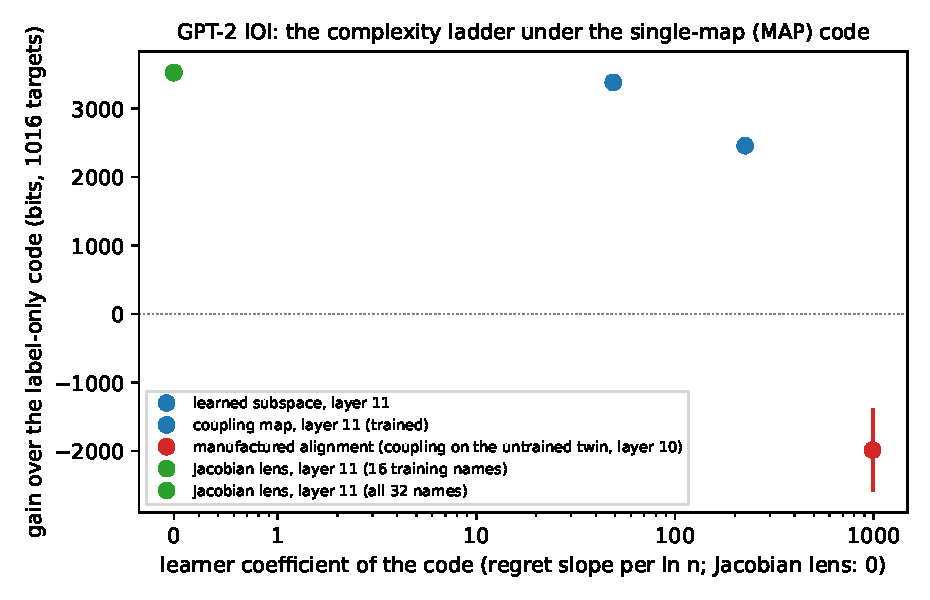
\includegraphics[width=0.8\textwidth]{../talk_slt/gpt2_complexity_ladder.pdf}
\caption{GPT-2 IOI, the complexity ladder under the single-map MAP code: gain over the label-only code against the learner coefficient of the code (regret slope per $\ln n$ on $n\le1024$; the Jacobian lens has none). The lens at coefficient 0 codes shortest; the learned subspace pays 49 without buying a shorter code; the coupling map pays 226 for a longer one; the manufactured alignment pays 988 and codes longer than label-only.}
\label{fig:ladder}
\end{figure}

\paragraph{The complexity ladder.} Figure~\ref{fig:ladder} places the four explanations of the same variable on one plot, gain over label-only against the learner coefficient of the MAP code (Section~\ref{sec:coef}). The lens sits at coefficient 0 with the shortest code of all; the learned subspace pays its coefficient of 49 without buying a shorter code; the coupling map on the trained network and the manufactured alignment pay 226 and 988 for longer ones. This is the floor of the ladder: the shortest explanation of the indirect-object name in GPT-2 is one with no parameters at all, read off the network's own Jacobian, and the code finds it so; what the code charges the learned explanations for is the Fisher-weighted search for a frame the network already supplies.

\paragraph{Four language models.} The lens was computed in the same way on Qwen2.5-0.5B (24 blocks), Pythia-1.4b (final checkpoint, 24 blocks) and Qwen3-1.7B-Base (28 blocks), on the IOI targets of every GPT-2 run (label-only 4324.5 bits), with the untrained twins under seed 7. Table~\ref{tab:jlensmodels} gives the loci around the readable range on all four models; the GPT-2 rows repeat Table~\ref{tab:jlens}.

\begin{table}[t]
\centering
\footnotesize
\caption{The Jacobian lens on four language models, IOI, variable \texttt{io}: condition number of $V_J$ (all 32 names), gain over the label-only code (4324.5 bits) with the frame from all 32 names and from the 16 training names, IIA on the i.i.d.\ split, and IIA on the 16 unseen names of the shifted split (all / train). Layer~0 fails on every model (IIA 0.07, gains $-3137$ to $-3723$ bits). The untrained twins fail at every locus.}
\label{tab:jlensmodels}
\resizebox{\textwidth}{!}{%
\begin{tabular}{llrrcc}
\toprule
model (blocks) & locus & $\mathrm{cond}(V_J)$ & gain, all / train & IIA iid & IIA unseen names, all / train\\
\midrule
GPT-2 small (12) & layer 10 & 119.3 & $+2821$ / $+2794$ & 0.80 / 0.78 & 0.78 / 0.06\\
 & layer 11 & 110.6 & $+3529$ / $+3525$ & 0.98 & 0.99 / 0.07\\
 & layer 12 & 7.6 & $+3626$ / $+3618$ & 1.00 & 0.99 / 0.07\\
 & untrained twin & 1.4--2.4 & $-844$ to $-855$ & 0.04 & \\
\midrule
Qwen2.5-0.5B (24) & layer 20 & 5.7 & $-3364$ / $-3366$ & 0.07 & 0.06 / 0.06\\
 & layer 22 & 4.0 & $+3334$ / $+3331$ & 0.94 & 0.90 / 0.06\\
 & layer 24 & 3.6 & $+3662$ / $+3657$ & 1.00 & 1.00 / 0.06\\
 & untrained twin & 1.4--2.9 & $-1033$ to $-1065$ & 0.03--0.06 & \\
\midrule
Pythia-1.4b (24) & layer 16 & 4.1 & $+2145$ / $+2143$ & 0.53 / 0.54 & 0.67 / 0.06\\
 & layer 18 & 3.3 & $+3498$ / $+3495$ & 1.00 & 1.00 / 0.06\\
 & layer 20 & 3.2 & $+3662$ / $+3659$ & 1.00 & 1.00 / 0.06\\
 & layer 24 & 2.8 & $+3715$ / $+3714$ & 1.00 & 1.00 / 0.06\\
 & untrained twin & 1.2--1.8 & $-1022$ to $-1070$ & 0.00--0.01 & \\
\midrule
Qwen3-1.7B-Base (28) & layer 22 & 5.4 & $-1046$ / $-1063$ & 0.08 & 0.07 / 0.06\\
 & layer 26 & 4.0 & $+3405$ / $+3406$ & 0.94 & 0.92 / 0.06\\
 & layer 28 & 3.4 & $+3593$ / $+3589$ & 0.98 & 0.99 / 0.06\\
 & untrained twin & 1.2--3.4 & $-1180$ to $-1211$ & 0.04--0.05 & \\
\bottomrule
\end{tabular}}
\end{table}

The parameter-free alignment is faithful at the last two to four layers of every model: GPT-2 layers 11--12 (IIA 0.98--1.00), Qwen2.5-0.5B layers 22--24 (0.94--1.00), Pythia-1.4b layers 18--24 (1.00) and Qwen3-1.7B layers 26--28 (0.94--0.98). There it codes the targets 3330--3715 bits shorter than label-only. It fails on every untrained twin (IIA 0.00--0.06, codes 1020--1210 bits longer than label-only on the three newer models). The frame built from all 32 names generalises to the 16 unseen names (0.90--1.00) wherever it is faithful; the training-name frame never does (0.06). Generalisation across names is a property of which directions are in the frame on every model, not only on GPT-2. The condition number of $V_J$ is 2.8--4.0 at the faithful loci of the newer models against 68--121 at GPT-2's layers 9--11: GPT-2's name directions are far less orthogonal. Where a learned subspace was scored at the same locus, the lens again codes shorter: on Qwen3-1.7B $+3593$ at layer~28 and $+3405$ at layer~26 against $+3042\pm3$ and $+3001\pm4$ for the learned subspace under the mixture (Table~\ref{tab:ioilm}), and on the final Pythia-1.4b checkpoint 663 bits at layer~20 against the learned subspace's 910 bits under the MAP code (Table~\ref{tab:pythia}). The Jacobian-lens hypothesis holds on all four models.


\section{Discussion, limitations and open questions}
\label{sec:limits}

This section states what is known at present about the open points the results raise, and what remains open.

\subsection{Limitations and open questions}

\paragraph{A complexity charge for the map family.} The layer-10 adversary on GPT-2 gains $+704\pm63$ bits over the label-only code under the canonical mixture learner (Section~\ref{sec:adversary}): a fixed-budget plug-in code does not charge for the $1.9$~M parameters of the coupling map in the way a Bayes or Laplace code over the map family would, through $\lambda\log n$ and the prior. We pursued such a charge in three steps. The Laplace learner, validated on the oracle (Section~\ref{sec:gauge}), fails on the saturated readouts of trained networks: its Gaussian collapses onto the prior, and the repaired, sampled code is a MAP code with a tunable hedge (Section~\ref{sec:bayescode}). On GPT-2 the absolute verdict on the adversary is then decided by whether one map or four are averaged, and the hedge at affordable chain lengths moves about 40 bits (Section~\ref{sec:learner}). Finally, a genuine Bayes code of the subspace family, run by HMC on InterpBench, is longer than the label-only code for the \emph{valid} alignment at 1024 targets, and the Hessian and empirical Fisher of the GPT-2 subspace loss show why: a regular family with nominal $\lambda=6016$ and a Fisher two per cent of its Hessian (Section~\ref{sec:coef}). At the widths of InterpBench and GPT-2 the Bayes learning coefficient of an alignment family is therefore not the complexity that makes an explanation short; the plug-in's $\tfrac12\mathrm{tr}(FH^{-1})$ is. On the 32-wide MLP of hierarchical equality the Bayes code is affordable, shorter than the plug-in, and charges the coupling family that the plug-in accepts (Section~\ref{sec:coef:ladder}); where along the ladder the crossover lies has not been measured. The next step is to report that quantity, or the regret slope that estimates it, as a summary column for every configuration rather than to build a Bayes code. Whether a converged posterior over the $1.9$~M coupling parameters would charge the adversary remains open; the chain lengths it would need are beyond these runs.

\paragraph{The learning-coefficient hypothesis on trained networks.} Where $\lambda$ is known, the hypothesis holds for the Bayes code: on reduced-rank regression the gains between two families that both contain the truth grow like $\Delta\lambda\ln n$, and the batching correction holds for a singular family (Section~\ref{sec:coef:rrr}). On the trained testbeds it has been examined through the regret of the MAP code. On InterpBench case~18 ($\dv=4$ and $\dv=1$) no $\lambda\ln n$ regime appears up to $n=1024$ (Section~\ref{sec:ha3ib:ib}), which is the interpolation regime of the map; beyond it the growth resumes, at a coefficient of roughly 45 against the nominal 512 on the run with 8192 targets, and at 23--42 on the runs to 32768 targets, still rising slowly with the fit range (Table~\ref{tab:ha3ib32768}). Whether it settles is open. The direct test of the hypothesis between two equivalent configurations on InterpBench, a Laplace code at $\dv=4$ against $\dv=8$, where the plug-in codes agree to $13\pm14$ bits, was originally planned and has not been run; the MAP-code runs at $\dv=4$ and $\dv=1$ were made instead. The SGLD estimator of the local learning coefficient, which reads $\lambda$ on reduced-rank regression, does not converge on the InterpBench transformer (Section~\ref{sec:ha3concl}). On the oracle the Bayes code's slope approaches its learning coefficient $k/2+(11-k)/4$ only with 16384 targets, from below on $n\le2048$; a run to 65536 targets that tests this against the nominal value is pending (Section~\ref{sec:coef:oracle}). On GPT-2 the plug-in prediction $\tfrac12\mathrm{tr}(FH^{-1})$ has been checked against the measurement at layer~11 only; the measurements at layers 10 and 12 and the Hessian at $\dv=64$ are pending (job 1820081).

\paragraph{Larger language models and MIB addition.} The runs on Llama-3.1-8B, Qwen2.5-3B, the Pythia-1.4b checkpoints and MIB addition have one seed each. The significance clause of the decisive-gain rule cannot be applied to them, and their statistical statements are the anytime ones. The manufactured-alignment arm on Qwen3-1.7B is still running (jobs 1814205--1814207). Gemma-2-2b IOI has been swept but not scored, because its coupling map needs a smaller learning rate. MIB addition has no distribution-shifted split, and the benchmark's other tasks need prompts of variable length, which the network adapter does not yet support. On Llama-3.1-8B no 16-dimensional subspace realises the carry at any of seven layers although a probe decodes it perfectly; whether a wider subspace or another position does is open. The Pythia series has one seed per checkpoint and omits checkpoints 32000 and 64000.

\paragraph{The disjoint-name failure.} No subspace map on GPT-2 transfers to unseen names: the shifted IIA of the valid hypotheses is 0.1 (chance for 16 names) at every width below $\dv=256$ in the sweep, the same as the adversary's 0.00. The distribution-shift test of Sutter et al.\ \cite{sutter2025} therefore does not separate the valid alignment from the manufactured one on this testbed, and the separation reported in Section~\ref{sec:adversary} rests on the code and on the distortion bound. The Jacobian lens shows that the failure is a matter of which directions are in the frame: the lens built from all 32 names transfers (shifted IIA 0.99), the lens built from the 16 training names fails like the learned map (0.07; Section~\ref{sec:jlens}), and the same holds on all four language models of Table~\ref{tab:jlensmodels}. Whether a larger $\dv$, a different position, or a name-invariant variable (the \texttt{order} variable of the IOI algorithm) gives a transferring learned alignment is open.

\paragraph{The noise floor between two random initialisations.} The comparative form of the rejection criterion compares the adversary on the untrained twin (seed 7) against the same map on a second twin (seed 8). On GPT-2 at layer~10 the two differ by $+349\pm195$ bits with per-seed values of $+702$, $+30$ and $+316$: the comparison is dominated by variance from the pair of initialisations, and three seeds cannot resolve it. More seeds and more twin initialisations are needed before the comparative form can be called a reliable test. A code that charges for the map is not a remedy at present: the sampled code at affordable chain lengths does not charge (Section~\ref{sec:learner}), and a genuine Bayes code charges valid alignments as well (Section~\ref{sec:coef:consequences}). Second twins at layers 6, 11 and 12 were not run.

\paragraph{The wrong-locus rule.} The wrong-locus control was first chosen as the locus at which a held-out probe for $V$ is least accurate. On InterpBench case~52, whose variable is a copy of the input token, decodable with accuracy 1.0 at the embedding and 0.91--0.96 downstream, that rule selected the locus of the valid hypothesis (Section~\ref{sec:ib52}). It was replaced, post hoc and logged as such, by a causal rule: the wrong locus is the locus at which the hypothesis's own map family attains the lowest held-out IIA (Section~\ref{sec:setup}). The causal rule reproduces the probe rule's choices on hierarchical equality, InterpBench cases 18 and 7 and GPT-2, and selects \texttt{resid\_1} on case~52. For copy variables the notion both rules operationalise, a locus before $V$ is computed, does not exist, and the causal rule replaces it by a locus at which the counterfactual cannot be realised. Having been adopted after the failure was seen, the causal rule has not yet been applied to a testbed chosen after it was fixed.

\paragraph{Variables that determine the output.} On InterpBench and IOI the aligned variable fixes the output by itself, and the counterfactual target is the source's own output: on case~18 the output is a function of \texttt{freq} alone, case~7's variable is the output, case~52's is a copy of the input token, and IOI's \texttt{io} is the source's answer, aligned at the final position (Sections~\ref{sec:tb:ib} and~\ref{sec:tb:ioi}). An interchange at the valid loci is then close to patching the output, and on these testbeds the evidence is carried by the controls (untrained twin, wrong locus, manufactured alignment): they are positive controls of the instrument, not tests of whether the code identifies an intermediate variable distinct from the output. Among the testbeds only hierarchical equality ($V_1=[a=b]$, with output $[V_1=V_2]$) and the carry of MIB addition, whose counterfactual combines the source's carry with the base's digit sums (one seed per model), test such a variable.

\paragraph{Other open points.} The other-map-family comparison is not a criterion of the preregistered evaluation and goes against the valid rotation on hierarchical equality ($-81\pm15$ bits at $h_1$) and on InterpBench case~52 (Section~\ref{sec:ib52}); the evaluation does not say what should happen when two faithful families of different expressiveness are compared. A code that charges map complexity is the natural resolution, and Section~\ref{sec:coef} indicates that the relevant charge is the plug-in's Fisher-weighted coefficient rather than a Bayes $\lambda$. The unmapped-variable test of Méloux et al.\ is not realised by our CAE: for a single-variable alignment on hierarchical equality the complement legitimately carries $V_2$, the complement interchange is the mapped one with base and source exchanged, and the CAE equals $1-\mathrm{IIA}$; a test on genuinely unmapped coordinates needs $V_2$ aligned as well. The subspace-illusion check covers only the learned subspaces on IOI, split by local sensitivity rather than by a row space; the coupling maps and the other testbeds are not checked (Section~\ref{sec:res:illusion}). On InterpBench cases 18 and 7 the wrong-locus control is a locus at which the map reaches IIA 0.2--0.5 only; on hierarchical equality the input locus was first chosen as merely the least decodable one, and the causal rule confirms it (attainable IIA 0.50 at the input against 0.99 at $h_1$ and 0.73 at $h_2$).

\subsection{Conclusion}
\label{sec:conclusion}

On all testbeds the valid alignments code decisively shorter than the label-only reference, their untrained twins and the wrong locus (for example $+506\pm19$ bits over label-only on hierarchical equality, $+983\pm11$ on InterpBench case~18 and $+3302\pm3$ at layer~11 of GPT-2). The manufactured alignment on GPT-2 reaches IIA 0.86 and is accepted by the accuracy baseline, but at layer~6 it codes no shorter than label-only ($+60\pm138$ bits); at layer~10 its absolute verdict depends on the learner ($+704\pm63$ bits under the mixture of four, about 1000 to 2000 bits longer than label-only under single-map learners; Section~\ref{sec:learner}), while the comparison with the valid alignment holds under every learner. Equivalent loci are ordered by faithfulness, and none of this holds unless every predictor codes the observed, noisy label law.

The verdicts carry over without retuning. In Llama-3.1-8B, Qwen2.5-3B and Qwen3-1.7B the valid IOI alignment gains 3000--3130 bits over label-only; on the two single-seed models the manufactured alignment codes 1700--1830 bits longer than label-only and at the strongest locus the coupling family on the trained network is 1440--1670 bits behind the subspace at an IIA 0.05 lower. On MIB's two-digit addition the model's own answer is the reference: the code finds the carry in a linear subspace of Gemma-2-2b at layer~20 and only through the non-linear family in Llama-3.1-8B at layer~24, ranking the two families in opposite orders and each time in favour of the faithful one. Along the training of Pythia-1.4b the code appears with task competence and keeps shortening after the accuracy saturates.

Beyond the preregistered evaluation the results say three things. The score orders explanations of a variable by the plug-in's Fisher-weighted complexity $\tfrac12\mathrm{tr}(FH^{-1})$, a learner coefficient that is 45--50 for the valid GPT-2 subspace against a nominal Bayes coefficient of 6016, that stays at 49--79 as the subspace dimension grows from 4 to 64, and that separates valid from manufactured alignments twentyfold. The Bayes learning coefficient of an alignment family is real and exactly measurable where $\lambda$ is known (reduced-rank regression, the oracle), but on trained networks as wide as InterpBench and GPT-2 it charges for prior mass along noise-free directions and makes even the valid alignment's code longer than label-only; on the 32-wide MLP of hierarchical equality it is affordable, gives the shorter code and charges the expressive family. On the oracle the Bayes code's slope reaches the learning coefficient $k/2+(d-1-k)/4$ with 16384 targets, which counts the directions the data do not occupy as quartic, while the plug-in's stays at $\tfrac12\mathrm{tr}(FH^{-1})=k/2$. And the shortest explanation of the indirect-object name in GPT-2, and in every other language model where the lens and a learned subspace were both scored, is the parameter-free Jacobian lens, at learning coefficient 0, and the code finds it so. What remains open at this scale is whether the plug-in coefficient settles on InterpBench beyond 32768 targets, whether the comparative adversary criterion can be made reliable with more initialisations, whether a name-invariant variable gives a transferring alignment, whether the plug-in prediction holds at GPT-2's layers 10 and 12 (pending), and how the score behaves on the MIB tasks that need prompts of variable length.
\appendix

\section{Hyperparameters}
\label{app:hyper}

Tables~\ref{tab:hyper}--\ref{tab:hyper:other} list the settings of every learner, map family and analysis. Unless stated otherwise they apply to all runs on hierarchical equality (HEQ), InterpBench (IB) and GPT-2 IOI.

\begin{table}[htbp]
\centering
\footnotesize
\caption{Schedule, channel and learners.}
\label{tab:hyper}
\begin{tabular}{p{0.24\textwidth}p{0.70\textwidth}}
\toprule
setting & value\\
\midrule
schedule & geometric, ratio $r=2$, first boundary 8, block ends $8,16,\dots,1024$ (7 blocks, 1016 coded targets); larger-$n$ runs continue to 8192 or 32768\\
final fit & every learner is refitted once on all targets after the prequential pass\\
channel & randomized response, $\varepsilon=0.05$, uniform over $K$ classes; every predictor codes $(1-\varepsilon)p+\varepsilon/K$\\
targets & 1024 training targets (seed 1); i.i.d.\ split 1000 pairs (seed 2); shifted split 1000 pairs (seed 3; HEQ and IOI only)\\
label-only code & Dirichlet$(1,\dots,1)$--categorical posterior predictive, frozen at block boundaries\\
\midrule
plug-in learner & fresh map at every block (cold start); Adam, no weight decay; 400 steps; minibatch $\min(256,\text{prefix})$ drawn with replacement; loss: mean negative log observed-law probability; learning rate $10^{-2}$ (HEQ and IB rotation and coupling; GPT-2 subspace), $10^{-3}$ (GPT-2 coupling)\\
mixture of four (canonical) & four plug-in members with independent seeds, equal-weight average of their observed-law predictive distributions; rotation members all start at the identity, subspace and coupling members at independent random initialisations; map size and distortion bound reported for the first member\\
manufactured alignment & coupling map on the untrained twin: HEQ and IB width 64, 2 blocks, 400 steps, learning rate $10^{-2}$; strong version width 256, 4 blocks, 4000 steps, $10^{-2}$; GPT-2 width 512, 4 blocks, 4000 steps (also 16{,}000), $10^{-3}$\\
wrong-locus rule & per locus two cold-start single-map plug-in fits (seeds 0 and 1) on all 1024 training targets; attainable IIA = best i.i.d.\ IIA; lowest wins, ties within 0.02 go to the earliest locus\\
\midrule
MAP learner & objective: negative log-likelihood of the prefix plus $\tfrac\alpha2\|\theta\|^2$, $\alpha=0.01$ (oracle: 1); IB subspace: L-BFGS (step 1, at most 100 iterations, strong-Wolfe line search, history 20), warm start from the previous block, fallback to Adam for 400 steps if the objective or parameters become non-finite; GPT-2, the larger language models and MIB (all families) and IB coupling: Adam on the mean loss with the prior as decoupled weight decay $\alpha/n$, the configuration's steps, learning rate and minibatch of 256, cold start; subspace frame re-orthonormalised after every step and after the fit. On the subspace family the prior changes only the frame's scale, a gauge direction, so the learner is a maximum-likelihood single-map (plug-in) learner; on coupling maps the decay per Adam step is at most $1.25\times10^{-6}$ (Section~\ref{sec:score:learners})\\
Laplace Gaussian (superseded) & $\mathcal N(\theta_{\rm MAP},(H+\alpha I)^{-1})$, exact Hessian up to 2000 parameters, otherwise diagonal empirical Fisher on 256 examples\\
MAP + Langevin & 200 Langevin steps from the MAP, minibatch 512, gradient of $n\cdot(\text{mean loss})+\text{prior}$, step $\eta\,\sigma_T^2$ per parameter tensor $T$ with $\sigma_T$ the standard deviation of $T$ at the MAP (floor $10^{-3}$), no preconditioning; samples evenly spaced over the second half; 8 samples (GPT-2), 16 (IB default); relative step $\eta=10^{-5}$ (default) or $10^{-4}$ (GPT-2 runs)\\
HMC Bayes code & $\mathcal N(0,1)$ prior on the raw map parameters; full-batch energy over the prefix; 4 chains, each started from a prior draw followed by 200 Adam steps (learning rate $10^{-2}$); 200 warm-up iterations with the step (initially $10^{-2}$) multiplied by 1.05 on acceptance and 0.9 on rejection; 100 samples per chain, keeping every second state; 20 leapfrog steps (HEQ, IB), 10 (oracle); on HEQ and IB the chains restart at every block, on the oracle they continue across blocks; predictor: average of the sampled maps' predictive distributions\\
\bottomrule
\end{tabular}
\end{table}

\begin{table}[htbp]
\centering
\footnotesize
\caption{Map families and their parameter counts.}
\label{tab:hyper:maps}
\resizebox{\textwidth}{!}{%
\begin{tabular}{lrrrr}
\toprule
testbed (width $d$, $\dv$) & rotation & subspace & coupling ($2\times64$) & strong ($4\times256$)\\
\midrule
HEQ ($d=32$ at $h_1,h_2$; 16 at input; $\dv=4$) & 496 (input: 120) & -- & 4{,}720 & 34{,}288\\
IB 18 ($d=260$; $\dv=4$, 8) & 33{,}670 & 1{,}040 / 2{,}080 & 67{,}078 & 300{,}934\\
IB 7 ($d=170$; $\dv=4$) & 14{,}365 & -- & 36{,}253 & --\\
IB 52 ($d=40$; $\dv=4$) & 780 & -- & 6{,}028 & --\\
GPT-2 ($d=768$; $\dv=16$) & -- & 12{,}288 & \multicolumn{2}{r}{coupling $4\times512$: 1{,}869{,}440}\\
oracle ($d=6$ or 12; $\dv=1$) & -- & 6 or 12 & -- & --\\
\bottomrule
\end{tabular}}

\medskip
\begin{minipage}{0.94\textwidth}\footnotesize
Rotation: $Q=\exp(S)$, $d(d-1)/2$ parameters, initialised at the identity. Subspace: $d\times\dv$ frame with $\mathcal N(0,1)$ initialisation, completed by QR with a fixed random complement. Coupling: blocks $x_2\leftarrow x_2+W_2\,\mathrm{ReLU}(W_1x_1+c_1)$ on alternating halves (split at $\lfloor d/2\rfloor$), default initialisation with both weight matrices scaled by 0.1, followed by a rotation initialised at the identity; the GPT-2 coupling map's rotation alone has 294{,}528 parameters. Interchange: $\phi^{-1}(z_V(\text{source}),z_\perp(\text{base}))$ with $z_V$ the first $\dv$ coordinates.
\end{minipage}
\end{table}

\begin{table}[htbp]
\centering
\footnotesize
\caption{Networks, synthetic testbeds and analyses.}
\label{tab:hyper:other}
\begin{tabular}{p{0.24\textwidth}p{0.70\textwidth}}
\toprule
setting & value\\
\midrule
HEQ network training & Adam, learning rate $10^{-2}$, minibatch 128 with replacement, cross-entropy, 4000 steps on 20{,}000 inputs from vocabulary $\mathcal A$; checkpoints at 0, $2^0,\dots,2^{11}$ and 4000\\
untrained twins & HEQ: step-0 checkpoint (first twin); uniform $\pm1/\sqrt{\text{fan-in}}$ re-draw with seed 8 (second twin). IB: weights $\mathcal N(0,\sigma^2)$ with the model's initialisation scale, biases 0, seeds 7 and 8. GPT-2: standard library initialisation under seeds 7 and 8\\
\midrule
oracle & noise rate 0.1; subspace map $\dv=1$; MAP: L-BFGS with at most 100 iterations, prior precision 1, warm start; geometric schedule of ratio 1.25 from 16; slopes on $n\ge256$; pool of $3n$ inputs; no learner channel unless stated\\
oracle LLC & tempered posterior $\beta=1/\ln n$; Langevin step $10^{-4}$ (also $10^{-5}$), localisation 10 (also 100), 1000 steps, 4 chains; MAP by L-BFGS with at most 300 iterations, cold start\\
reduced-rank regression & least-squares plug-in from a prefix of $N+2$; Bayes code by HMC on the sufficient statistics: 64 chains of 200 samples (every second state kept), 300 warm-up iterations, 20 leapfrog steps, chains initialised at a balanced factorisation of the least-squares matrix plus $0.1\times$ prior noise, step $\min(0.05,0.5/\sqrt{\lambda_{\max}(S_{xx})})$ adapted by 1.05 / 0.9 around acceptance 0.7 during warm-up; LLC at the MAP (gradient descent from 8 restarts, 2000 iterations): 32 Langevin chains, $\beta=1/\ln n$, 4000 steps, step $10^{-4}$, localisation 1; schedule check: 32 chains of 60 samples, 100 warm-up iterations\\
\midrule
online probe code (HEQ) & multinomial logistic regression with intercept, ridge $10^{-2}$, L-BFGS-B from zero, at most 200 iterations, refitted at every block\\
CAE (HEQ) & 1000 i.i.d.\ pairs, final map; complement interchange scored against $A(s;V_1\leftarrow V_1(b))$; random-direction swap: a random rotation (seed 0)\\
D1 (HEQ) & locus states of the 795 distinct base inputs among the 1024 training targets; margin ratios, no permutation null\\
D2 (HEQ) & up to 100 triples (seed 0); segment sensitivity at 3 points by 30 power iterations; $\Lambda_{\rm nat}$ = median Jacobian norm over 64 random pool states\\
\midrule
Jacobian lens (GPT-2; also Qwen2.5-0.5B, Pythia-1.4b, Qwen3-1.7B-Base) & J-vectors: gradient of each name's logit at the final position with respect to the locus state at the final position, averaged over the first 1000 pool prompts (minibatch 64, accumulated in 64-bit floating point); frame: left singular vectors of the unit J-vectors with singular value above $10^{-6}$ times the largest, completed by QR with a seed-0 random matrix; no fitted parameters\\
Jacobian consistency & 500 triples from the i.i.d.\ split (seed 5); reference maps: one subspace map ($\dv=16$, 400 Adam steps, learning rate $10^{-2}$, seed 0, all 1024 targets) and one coupling map ($4\times512$, 4000 steps, $10^{-3}$, seed 0) on the twin\\
curvature (GPT-2) & layer 11, $\dv=16$ subspace (also layers 10 and 12 at $\dv=16$ and layer 11 at $\dv=4$ and 64, with the held-out Fisher); MAP by L-BFGS (at most 100 iterations, prior precision 0.01, cold start, seed 0) on the 1024 training targets; dense Hessian of the mean loss from 12{,}288 Hessian-vector products; empirical Fisher = mean outer product of the per-example gradients, on the 1024 training targets or the 1000 i.i.d.\ targets, evaluated in the Hessian's eigendirections\\
\midrule
larger language models (IOI) & Llama-3.1-8B and Qwen2.5-3B in bfloat16, Qwen3-1.7B-Base and Pythia-1.4b in float32; subspace $\dv=16$ (learning rate $10^{-2}$, 400 steps), coupling $4\times512$ ($10^{-3}$); single-map MAP learner (AdamW, prior precision 0.01, cold start, no samples) for Llama-3.1-8B, Qwen2.5-3B and Pythia-1.4b, mixture of four for Qwen3-1.7B-Base; manufactured alignment 4000 steps (Pythia-1.4b: 400) on the seed-7 twin\\
MIB addition & prompts starting ``Q: How much is'' with two-digit operands; MIB training split (training targets, i.i.d.\ split) and validation split; alphabet: distinct first tokens of ``0''--``198''; bfloat16; maps and learner as in the row above (MAP learner); manufactured alignment 4000 steps at layer 24 (Llama-3.1-8B) and 20 (Gemma-2-2b)\\
HMC on hierarchical equality & rotation family at $h_1$, $h_2$ and the input, coupling $2\times64$; the HMC settings of Table~\ref{tab:hyper}; five seeds\\
\bottomrule
\end{tabular}
\end{table}

\section{Correspondence with the project record}
\label{app:labels}

The results were produced under internal names that appear in the code, the result directories and the project's progress log. Table~\ref{tab:labels} maps them to the names used in this paper, so that every reported number can be traced to its source (Appendix~\ref{app:provenance}).

\begin{table}[htbp]
\centering
\footnotesize
\caption{Internal labels of the project record and their names in this paper.}
\label{tab:labels}
\begin{tabular}{p{0.30\textwidth}p{0.64\textwidth}}
\toprule
project record & this paper\\
\midrule
\raggedright Stage~1 & the score of this paper (``alignment sample efficiency''); Stage~2, coding the network's own behaviour, is not part of it\tabularnewline
\raggedright gate G-A1 & the preregistered evaluation (Sections~\ref{sec:prereg} and~\ref{sec:gate}); \file{preregistration/G-A1.md} is its preregistration file\tabularnewline
\raggedright H-A1 & the hypothesis behind the evaluation: the gains reject manufactured alignments that pass distribution-shifted held-out tests and the causal abstraction error, while retaining valid explanations up to equivalence\tabularnewline
\raggedright H-A2 & the competence-onset hypothesis (Section~\ref{sec:tb:heq}; on a language model, Section~\ref{sec:res:pythia})\tabularnewline
\raggedright H-A3 & the learning-coefficient hypothesis (Section~\ref{sec:regretdef})\tabularnewline
\raggedright H-A8, H-A9 & the hypotheses behind the stretch and separation diagnostics D1--D2 (Section~\ref{sec:score:faith})\tabularnewline
\raggedright H-A10 & the Jacobian-lens hypothesis (Section~\ref{sec:jlens})\tabularnewline
\raggedright T3 (proof target) & the batching correction (Section~\ref{sec:regretdef})\tabularnewline
\raggedright T4 (proof target) & the question when a learner's coefficient $\kappa$ equals the Bayes $\lambda$ (Sections~\ref{sec:regretdef} and~\ref{sec:coef})\tabularnewline
\raggedright criterion 1 / 2 / 3 / 4 / 5 & existence / rejection / retention / equivalence / separation (Section~\ref{sec:prereg})\tabularnewline
\raggedright ``the toy'' & hierarchical equality, the MLP testbed\tabularnewline
\raggedright the user's decision & the authors' decision (amendments are marked post hoc)\tabularnewline
\raggedright run suffix \texttt{\_rr} & runs with the randomized-response channel in every predictor (all reported verdict runs)\tabularnewline
\raggedright \texttt{mix4} & the mixture-of-four learner\tabularnewline
\raggedright \texttt{dv4}, \texttt{dv8}, \texttt{dv1} & subspace width $\dv=4$, 8, 1\tabularnewline
\raggedright \texttt{map}, \texttt{map0} & the single-map MAP learner (no posterior samples)\tabularnewline
\raggedright \texttt{sgld4}, \texttt{sgld5} & MAP + Langevin with relative step $10^{-4}$, $10^{-5}$\tabularnewline
\raggedright \texttt{sgld4map} & the same with the step scale measured at the MAP\tabularnewline
\raggedright \texttt{plugin1} & the plug-in learner with one member\tabularnewline
\raggedright \texttt{hmc} & the Bayes code by HMC\tabularnewline
\raggedright \texttt{twin=8}, \texttt{second\_twin\_seed} & the second untrained twin\tabularnewline
\raggedright \texttt{locus=}$\cdot$, \texttt{map=coupling}, \texttt{/untrained} & the wrong-locus, other-family and untrained-twin controls of a hypothesis\tabularnewline
\raggedright \texttt{least\_decodable\_locus} / \texttt{least\_intervenable\_locus} & the probe rule / the causal rule for the wrong locus\tabularnewline
\raggedright \texttt{SubspaceMap}, \texttt{Rotation}, \texttt{AdditiveCoupling} & subspace map, rotation, coupling map\tabularnewline
\raggedright \texttt{MixtureAlignmentLearner}, \texttt{GradientAlignmentLearner}, \texttt{LaplaceAlignmentLearner}, \texttt{HmcAlignmentLearner} & mixture-of-four, plug-in, MAP / Laplace / MAP + Langevin, HMC learners\tabularnewline
\raggedright \texttt{NoiseChannel} & the observed-law channel~\eqref{eq:channel}\tabularnewline
\raggedright \texttt{k\_relevant}, \texttt{beta\_scale}, \texttt{v\_continuous}, \texttt{v\_margin} & readable directions $k$, sharpness $s$, continuous $v$, margin $m$ of the oracle\tabularnewline
\raggedright \texttt{--sgld-lr} & the relative Langevin step $\eta$\tabularnewline
\raggedright tier-2 models & the larger language models (Sections~\ref{sec:tb:ioilm} and~\ref{sec:res:ioilm})\tabularnewline
\raggedright MIB arithmetic, \texttt{--task arith} & two-digit addition of the MIB causal-variable track (Sections~\ref{sec:tb:mib} and~\ref{sec:res:mib})\tabularnewline
\raggedright trivial floor & the model's own answer on the base, measured by the wrong-locus control at layer~0 (Section~\ref{sec:tb:mib})\tabularnewline
\raggedright competence-onset series, \texttt{pythia\_ckpt} & Pythia-1.4b along training (Section~\ref{sec:res:pythia})\tabularnewline
\raggedright the ladder toy / InterpBench / GPT-2 & the ladder in $n$ against $\lambda$ (Section~\ref{sec:coef:ladder})\tabularnewline
\raggedright \texttt{laplace[\dots,S=0,adam,\dots]} & the single-map MAP learner with AdamW, no posterior samples (Sections~\ref{sec:learner} and~\ref{sec:tb:ioilm})\tabularnewline
\bottomrule
\end{tabular}
\end{table}

\section{Provenance of the reported numbers}
\label{app:provenance}
\sloppy

Every number in this paper was read from a file in the project repository or computed from the per-seed records stored there. This appendix gives, section by section, the file each number comes from, the job or commit that produced it where relevant, and the notes on discrepancies between sources. Paths are relative to the repository root. The package source is \file{src/bitsev/}; result directories are under \file{results/} (one \file{settings.json} and one record per configuration and seed in \file{records/}); human-readable summaries are under \file{reports/}; \file{PLAN.md} is the project's dated progress log, cited by entry date; \file{preregistration/G-A1.md} is the preregistration file; the research plan is \file{research_plan_synthesis_v7_2.tex} and \file{research_plan_synthesis_v7_3.tex} (identical in every passage cited here except the Jacobian-lens additions of version 7.3, which are also in \file{appendix_jlens.tex}). Job numbers are those of the cluster's batch scheduler; commit hashes refer to the repository's history. A general caveat: every runner rewrites \file{settings.json} on every invocation, including summary-only rebuilds and later wrong-locus re-runs, so fields such as \texttt{seeds} or \texttt{wrong\_locus} describe the last invocation; the records are authoritative where the two differ. Where a correction to the earlier record was verified against the code, it is noted as ``corrected from the earlier record''.

\subsection*{Sections~\ref{sec:intro} and~\ref{sec:background}}

The research question, the dilemma reading by minimax regret, the role of randomized response, the decomposition~\eqref{eq:gain} and its three regimes, the learner-coefficient statements and the e-value statements are from the research plan (version 7.3, Sections ``Background'', ``Stage 1: alignment sample efficiency'' (\texttt{sec:stage1}), ``What prequential scores measure'' and Appendix~B). The numbers in the introduction and the abstract are those of Sections~\ref{sec:results}--\ref{sec:jlens} and carry their provenance there. The description of the causal abstraction error follows the docstring of \file{src/bitsev/baselines/cae.py}; the attribution of hierarchical equality follows \file{notes/testbeds_survey.md} and the module docstring of \file{src/bitsev/testbeds/hierarchical_equality.py} (``Hierarchical equality (Geiger et al.)''). The research plan cites no source for randomized response, for SGLD, for HMC or for Ville's inequality; the references \cite{warner1965,wellingteh2011,li2016psgld,neal2011hmc,ville1939} were added for this paper and their bibliographic details have not been checked against the publications.

\subsection*{Section~\ref{sec:setup}: the score}

\paragraph{Score and schedule.} Definition: research plan, Section ``Stage 1: alignment sample efficiency'' (\texttt{sec:stage1}); \file{preregistration/G-A1.md}, ``The score''; schedule \texttt{codes/schedule.geometric}; prequential pass \file{src/bitsev/codes/prequential.py}; final fit \texttt{score\_configuration} in \file{src/bitsev/alignment/score.py}. Target construction: \texttt{make\_targets} and \texttt{randomized\_response} in \file{src/bitsev/alignment/targets.py}.

\paragraph{Channel.} \file{src/bitsev/alignment/targets.py}, class \texttt{NoiseChannel}: ``every predictor codes the observed label law $(1-\mathrm{rate})\,p(y)+\mathrm{rate}/K$ rather than the clean law $p(y)$ \dots\ without the channel each flipped label costs tens of bits against a correct alignment.''

\paragraph{Label-only code.} Values from the headers of \file{reports/stage1_toy/summary_dv4_mix4_rr.md}, \file{reports/stage1_interpbench/case18_summary_dv4_mix4_rr.md}, \file{case7_summary_dv4_mix4_rr.md}, \file{case52_summary_dv4_mix4_rr.md} and \file{reports/stage1_ioi/gpt2_summary_v2.md}. Corrected from the earlier record: the label-only code is the Dirichlet$(\alpha=1)$--categorical Bayes (posterior-predictive) code, not a plug-in (\texttt{label\_only\_learner} in \file{src/bitsev/alignment/controls.py}; \texttt{DirichletCategorical} with \texttt{alpha=1.0} in \file{src/bitsev/codes/conjugate.py}); \file{preregistration/G-A1.md} and the earlier write-up called it a plug-in. The relabelling-invariance statement is proof target T2 of the research plan (status there: proved).

\paragraph{Map families and learners.} \file{src/bitsev/alignment/maps.py}, docstrings of \texttt{SubspaceMap}, \texttt{Rotation} and \texttt{AdditiveCoupling}; the distortion bound is research plan Appendix~D.8 (subsection ``Relation to the code lengths of Stage 1''). Mixture learner: \file{src/bitsev/alignment/learners.py}, class \texttt{MixtureAlignmentLearner} (the motivation in the text paraphrases its docstring); budget \file{preregistration/G-A1.md}, ``The score''; adoption as canonical \file{PLAN.md}, entries 2026-10-15 (afternoon, evening, decisions implemented). Learning rates and budgets are confirmed by the learner tags stored in the records, e.g.\ \texttt{mixture4:grad[rotation,cold,steps=400,lr=0.01,rr=0.05]}. Corrected from the earlier record: with the rotation family the four mixture members all start at the identity (\texttt{init\_scale=0.0}) and differ only in their minibatch sequences; subspace and coupling members have random initialisations. The MAP, Laplace, Langevin and HMC learners: \texttt{LaplaceAlignmentLearner} and \texttt{LaplaceBudget} in \file{src/bitsev/alignment/learners.py}, \file{src/bitsev/alignment/hmc.py}.

\paragraph{Controls.} Untrained twins: \texttt{reinitialised\_twin} in \file{src/bitsev/alignment/network.py}, \texttt{TLTransformer.reinitialised} in \file{src/bitsev/testbeds/tl_transformer.py}, \texttt{HFNetwork.reinitialised} in \file{src/bitsev/alignment/hf_network.py}. Corrected from the earlier record: on hierarchical equality the untrained twin is the step-0 checkpoint of the training run (\texttt{network\_at(net, run, 0)} in \file{src/bitsev/experiments/run_stage1_toy.py}, module docstring), not a seed-7 re-initialisation; the seed-8 second twin is a genuine re-initialisation. On InterpBench and GPT-2 the first twin is a seed-7 re-initialisation, as previously stated. Wrong locus: the probe rule is \texttt{probe\_accuracies} and \texttt{least\_decodable\_locus}, the causal rule \texttt{least\_intervenable\_locus} with the tolerance in \texttt{\_earliest\_within}, all in \file{src/bitsev/alignment/controls.py}; the copy-variable caveat is \file{PLAN.md}, entry 2026-10-15 (late); the redefinition is \file{PLAN.md}, entry 2026-10-19 (decision), and the change log of \file{preregistration/G-A1.md} (commits \texttt{d7d8454}, \texttt{b5177e3}). Corrected from the earlier record: the earlier write-up described the probe rule as the rule in force; the causal rule has been in force since 2026-10-19, and only case~52's wrong-locus records changed (recomputed by job 1812245; the superseded records are kept in \file{results/stage1_ib52_dv4_mix4_rr/records_superseded_probe_rule/}). The attainable IIA values quoted in the text are those of \file{PLAN.md} (entry 2026-10-19, decision) and \file{preregistration/G-A1.md}. The \file{settings.json} files record attainable IIA 0.498 / 0.99 / 0.727 (hierarchical equality, \file{results/stage1_toy_dv4_mix4_rr/wrong_locus.json}), 0.456 / 0.842 / 0.998 (case~18) and 0.168 / 0.992 / 0.999 (case~7), in agreement; for case~52 \file{results/stage1_ib52_dv4_mix4_rr/settings.json}, written by the recomputation job, records \texttt{resid\_0} 0.949, \texttt{resid\_1} 0.253, \texttt{resid\_2} 0.994, which differ from the 0.99 / 0.11 / 0.64 of the progress log but select the same locus. For GPT-2, \file{results/stage1_ioi_gpt2_v2/settings.json} records \texttt{"wrong\_locus": "layer6"}: it was written by the wrong-locus re-run job 1812247 before the 0.02-tolerance clause was added; under the rule as stated the choice is layer~0, which is what every GPT-2 record uses. Probe accuracies: \texttt{probe\_accuracy} in the same \file{settings.json} files. Manufactured alignment: \file{preregistration/G-A1.md}, ``Testbeds, hypotheses and controls''; parameter count from the status of criterion~2 there and from the records' \texttt{map\_params}.

\paragraph{Faithfulness measures and diagnostics.} \file{src/bitsev/alignment/score.py}, \texttt{Faithfulness} and \texttt{faithfulness}; \file{src/bitsev/baselines/probing_mdl.py} and \texttt{probe\_records} in \file{src/bitsev/experiments/run_stage1_toy.py}; \file{src/bitsev/baselines/cae.py}; \file{src/bitsev/diagnostics/separation.py} (D1) and \file{src/bitsev/diagnostics/stretch.py} (D2); stretch budget: research plan Appendix~D. Corrected CAE (complement prediction) and D1 (margin ratios on distinct bases): commit \texttt{bb77a66}; numbers from \file{reports/stage1_toy/diagnostics_corrected.txt} (table and ``Reading'' (1)--(3)), run \file{results/stage1_toy_dv4_mix4_rr_diag} (job 1827641), which repeats the fits of \file{results/stage1_toy_dv4_mix4_rr} with identical code lengths; the CAE and D1 values of the earlier record (CAE 0.2 against 0.5; permutation $p=0.0099$ everywhere) are superseded. Corrected from the earlier record: InterpBench has no shifted split; the runner copies the i.i.d.\ faithfulness into the ``shifted'' slot (\file{src/bitsev/experiments/run_stage1_interpbench.py}), so every ``shifted'' InterpBench value in the summaries equals the i.i.d.\ value.

\paragraph{Decisive gains.} \file{preregistration/G-A1.md}, ``Criteria'' (rule unchanged since the first draft, commit \texttt{1969de6}). The floors for cases 7 and 52 are 5\% of their label-only codes.

\paragraph{Anytime evidence.} Definition: function \texttt{summarise} in \file{src/bitsev/experiments/run_stage1_toy.py} (the index is the first crossing of $\log 100$ nats by the cumulative sum of the per-item loss differences, offset by the first boundary, maximised over seeds); the same definition precedes each gains table, e.g.\ in \file{reports/stage1_toy/summary_dv4_mix4_rr.md}. Values: \file{reports/stage1_toy/summary_dv4_mix4_rr.md}, \file{reports/stage1_interpbench/case18_summary_dv4_mix4_rr.md} and \file{case18_summary_dv8_mix4_rr.md}, columns ``peak evidence'' and ``rejects $\alpha=0.01$ by $n$''; the manufactured-alignment rows are \texttt{untrained/.../coupling} against \texttt{coupling/twin=8}. The caveat is \file{PLAN.md}, entry 2026-10-19 (later); \file{src/bitsev/codes/evalues.py}.

\paragraph{Regret and learner coefficients.} \file{src/bitsev/experiments/h_a3.py}, module docstring and \texttt{regret\_curve} (reference: \texttt{extra.final\_item\_nats}, optionally from a reference run given by \texttt{--reference-run}, with a check of equal target hashes); \file{src/bitsev/codes/gain.py}, \texttt{fit\_log\_slope} and \texttt{LogFit.corrected\_slope}; \texttt{batching\_factor} in \file{src/bitsev/codes/schedule.py}. Batching correction: research plan, proof target T3 and Appendix ``batch'' (Gaussian-mean check). Learner coefficients: research plan, ``What prequential scores measure'' and proof target T4. Learning-coefficient hypothesis: research plan, hypothesis H-A3. LLC: \file{src/bitsev/alignment/llc.py}.

\subsection*{Section~\ref{sec:testbeds}: testbeds, data and networks}

\paragraph{Targets.} \texttt{make\_targets} in \file{src/bitsev/alignment/targets.py}; \texttt{TargetSet.content\_hash} (sha256 over bases, sources, clean and noisy labels, variable, rate, $K$ and seed). Target hashes, all reproduced: hierarchical equality \texttt{ef53ae7ab6d7890b}, case~18 \texttt{39c60f6b5e9ca439}, case~7 \texttt{6fd5ea486de804ae}, case~52 \texttt{5db132df67c67ae7}, GPT-2 \texttt{927e660f3575b1b1}. Label counts and channel change rates recomputed from the target sets.

\paragraph{Hierarchical equality.} \file{src/bitsev/testbeds/hierarchical_equality.py} (\texttt{make\_disjoint\_vocabularies}, \texttt{sample}), \file{src/bitsev/testbeds/training.py} (\texttt{train\_classifier}), \file{src/bitsev/alignment/network.py} (\texttt{mlp}), \file{src/bitsev/alignment/algorithms.py} (\texttt{HierarchicalEquality}), \file{src/bitsev/experiments/run_stage1_toy.py} (\texttt{parse}, \texttt{build\_world}, \texttt{configurations}; seeds \texttt{default\_rng(20261014)} and \texttt{torch.manual\_seed(20261014)}). Reported run \file{results/stage1_toy_dv4_mix4_rr} (job 1762771). Training curve: \file{results/stage1_toy_dv4_mix4_rr/training.json}; held-out accuracies 1.000 and 0.9905 re-computed by re-running \texttt{build\_world}. Hypotheses and seeds: \file{preregistration/G-A1.md}, ``Testbeds, hypotheses and controls''. Competence-onset hypothesis: research plan, hypothesis H-A2.

\paragraph{InterpBench.} \file{src/bitsev/testbeds/interpbench.py} (download from the Hugging Face repository \texttt{cybershiptrooper/InterpBench}, licence CC-BY-4.0; \texttt{Tokens}; \texttt{\_build\_18}, \texttt{\_build\_7}, \texttt{\_build\_52}; \texttt{task\_accuracy}; \texttt{VERIFIED = \{"52","7","18"\}}), \file{src/bitsev/testbeds/tl_transformer.py} (re-implemented forward pass; docstring: ``matches TransformerLens 1.19 to 1e-3 on all four cases''), \file{src/bitsev/experiments/run_stage1_interpbench.py}. Architectures from the released configuration files; the training method of the released models from the benchmark's metadata (\texttt{training\_args}, e.g.\ \texttt{model\_pair = 'strict'}). Reported runs \file{results/stage1_ib18_dv4_mix4_rr} (job 1762772), \file{results/stage1_ib18_dv8_mix4_rr}, \file{results/stage1_ib7_dv4_mix4_rr} (job 1804344) and \file{results/stage1_ib52_dv4_mix4_rr} (job 1804343); their \file{settings.json} files record \texttt{task\_accuracy} 1.0, \texttt{coupling\_width} 64, \texttt{coupling\_blocks} 2, \texttt{map\_steps} 400, \texttt{members} 4, \texttt{seeds} 3. The case-18 variable and the circuit are those of \texttt{\_build\_18} and of the ground-truth edges stored in \file{settings.json} (e.g.\ \texttt{blocks.0.hook\_mlp\_out} $\to$ \texttt{blocks.1.hook\_mlp\_in}). Case~13 discarded: \file{PLAN.md}, entry 2026-10-15 (evening). Cases 7 and 52 were run on 2026-10-18 and 2026-10-19 (\file{PLAN.md}, entries of those dates).

\paragraph{IOI in GPT-2 small.} \file{src/bitsev/testbeds/ioi.py} (\texttt{TEMPLATES}, \texttt{NAMES}, \texttt{PLACES}, \texttt{OBJECTS}, \texttt{build\_prompts}, \texttt{IOIAlgorithm}), \file{src/bitsev/alignment/hf_network.py}, \file{src/bitsev/experiments/run_stage1_ioi.py} (\texttt{parse}, \texttt{build}, \texttt{\_targets\_within}, \texttt{main}; \texttt{--n-names 16}, \texttt{--layers 0 6 9 10 11 12}, seed \texttt{default\_rng(20261016)}). Main run \file{results/stage1_ioi_gpt2_v2} (jobs 1785940--1785942 for seeds 0--2 and 1796197--1796198 for seeds 3--4); adversary sweep \file{results/stage1_ioi_gpt2_adversaries} (jobs 1801917--1801919). Corrected from the earlier record: only 2 of the 5 templates survive the equal-token-length filter (template lengths 14, 14, 18, 16 and 15 tokens; of the 3214 kept prompts 1622 use ``gave a'' and 1592 ``gave the''), GPT-2 prompts carry no beginning-of-sequence token (GPT-2's tokenizer adds none), layer~0 is the token-plus-position embedding and layer~12 the state after the final layer normalisation (verified against the model's hidden states). Corrected from the earlier record: the main run has five seeds in its records; its \file{settings.json} says \texttt{seeds: 3} because it was last written by a re-run. Accuracy: \texttt{model\_ioi\_accuracy\_among\_names = 0.99609375} in \file{results/stage1_ioi_gpt2_v2/settings.json}, the argmax over the 32 name logits on the first 1024 pool prompts; the 99.7\% in \file{PLAN.md}, entry 2026-10-15 (decisions implemented), was an earlier check after a template fix on a different name set. The 32 names are a hand-picked list in the code; how they were chosen is not documented. The model is loaded without a pinned revision. Learner-specification sweep: \file{src/bitsev/experiments/ioi_map_sweep.py} (512 training targets, 500 evaluation pairs, seed 0), results \file{results/ioi_map_sweep/} (\file{sweep.json}, \file{sweep_layer6.json} and the per-layer \file{layer*/sweep.json}; job 1785790); the first GPT-2 run and the sweep's conclusions are \file{PLAN.md}, entries 2026-10-16 and 2026-10-16 (evening). The range 0.10--0.35 of the widest maps' shifted IIA is read from the per-layer sweep files.

\paragraph{Larger language models (Section~\ref{sec:tb:ioilm}).} \file{src/bitsev/alignment/hf_network.py} (module docstring: locus \texttt{layer}$\ell$ is the residual entering decoder layer $\ell$, $\ell=0$ the embedding output, $\ell=L$ the final post-norm state; \texttt{HFNetwork.reinitialised}, the untrained twin built by \texttt{from\_config} under the seed; the bfloat16 comment in \texttt{\_\_init\_\_}); \file{src/bitsev/experiments/run_stage1_ioi.py}. Widths and depths from the \texttt{hidden\_size} and \texttt{num\_hidden\_layers} fields of the models' \file{config.json} in the local Hugging Face cache. Run settings from \file{results/stage1_ioi_llama31_8b/settings.json}, \file{results/stage1_ioi_qwen25_3b/settings.json}, \file{results/stage1_ioi_qwen3_17b/settings.json} and \file{results/pythia_ckpt/step*/settings.json} (\texttt{model}, \texttt{revision}, \texttt{dtype}, \texttt{layers}, \texttt{learner}, \texttt{laplace\_samples} 0, \texttt{prior\_precision} 0.01, \texttt{adversary\_steps}, \texttt{adversary\_layer}, \texttt{token\_length}, \texttt{targets\_hash}, \texttt{model\_ioi\_accuracy\_among\_names}, \texttt{attainable\_iia}, \texttt{probe\_accuracy}); learner tags in the records, e.g.\ \path{laplace[subspace,alpha=0.01,S=0,adam,steps=400,cold,rr=0.05]} (Llama-3.1-8B, Qwen2.5-3B, Pythia-1.4b, MIB) and \path{mixture4:grad[subspace,cold,steps=400,lr=0.01,rr=0.05]} (Qwen3-1.7B-Base). Locus sweeps: \file{reports/stage1_ioi/map_sweep_llama31_8b.json}, \file{map_sweep_qwen25_3b.json}, \file{map_sweep_qwen3_17b.json}, \file{map_sweep_pythia14.json} and \file{map_sweep_gemma2_2b.json} in the same directory. \file{PLAN.md}, entries 2026-10-21 (strong adversaries, tier-2 sweeps; Llama-3.1-8B runs on the H100s; late; afternoon archive). \emph{Corrected from the report file:} \file{reports/stage1_ioi/tier2_models.txt} states that every model was run with the mixture-of-4 learner; the settings and the record tags show that Llama-3.1-8B and Qwen2.5-3B (and, as \file{reports/stage1_ioi/pythia14_checkpoint_series.txt} states, every Pythia checkpoint) were run with the single-map MAP learner, and only Qwen3-1.7B-Base with the mixture. The text follows the records.

\paragraph{MIB addition (Section~\ref{sec:tb:mib}).} \file{src/bitsev/testbeds/mib.py}: module docstring (prompt form, track variable, alphabet of distinct first tokens of ``0''--``198'', one token per answer for Llama~3, the first digit for Gemma), \texttt{build\_arithmetic} (the template filter and the six templates of different token lengths), \texttt{ArithmeticAlgorithm} (variables and output; the counterfactual for \texttt{carry}); \file{src/bitsev/experiments/run_stage1_ioi.py}, \texttt{\_build\_arith} (training-split prompts for the training targets and the i.i.d.\ split, validation-split prompts for the ``shifted'' split). Settings \file{results/stage1_arith_llama31_8b/settings.json} and \file{results/stage1_arith_gemma2_2b/settings.json} (\texttt{layers}, \texttt{dtype} bfloat16, \texttt{learner}, \texttt{adversary\_layer}, \texttt{model\_ioi\_accuracy\_among\_names} 0.985 and 0.993, which for this task is the accuracy on the answer token, \texttt{attainable\_iia}, \texttt{probe\_accuracy}). Label-only codes and target hashes: headers of \file{reports/stage1_mib/arith_llama31_8b_summary.md} and \file{reports/stage1_mib/arith_gemma2_2b_summary.md}. The trivial floor and the comparison with MIB's 52\% for DAS: \file{reports/stage1_mib/arithmetic.txt}, paragraph ``The trivial floor''. \file{PLAN.md}, entries 2026-10-21 (afternoon launches; MIB arithmetic; Llama-3.1-8B runs on the H100s; late; afternoon archive). \emph{Corrected from the report file:} the header of \file{reports/stage1_mib/arithmetic.txt} names the mixture-of-4 learner; both runs used the single-map MAP learner (settings and record tags).

\paragraph{Synthetic testbeds.} Oracle: \file{src/bitsev/testbeds/oracle.py} (\texttt{OracleNetwork}, \texttt{OracleAlgorithm}, \texttt{make\_oracle} and its docstring: ``the effective learning coefficient is \texttt{k\_relevant / 2} instead of \texttt{(d - 1) / 2}''; \texttt{true\_counterfactual\_log\_probs}; the \texttt{beta\_scale} factor in \texttt{OracleNetwork.\_\_init\_\_}; the \texttt{while v\_margin > 0} loop), \file{src/bitsev/experiments/oracle_lambda_sweep.py} (defaults \texttt{--d 12}, \texttt{--ks 1 2 4 7 11}, \texttt{--growth 1.25}, \texttt{--seeds 4}, \texttt{--eps 0.1}, \texttt{--n-min 256}, \texttt{--channel none}; help text of \texttt{--channel}), \file{tests/test_laplace_oracle.py} (gauge check), \file{PLAN.md}, entries 2026-10-15 (decisions implemented), 2026-10-19 (afternoon, night) and 2026-10-20. The command lines of the stored oracle sweeps were not saved; their settings ($d$, $k$, $n$, ratio, sharpness, margin) are inferred from the contents of the stored \file{sweep.json} files and from \file{reports/oracle/}; the margin control's six seeds are those listed in \file{reports/oracle/margin_control_per_seed.txt}. Reduced-rank regression: \file{src/bitsev/testbeds/rrr.py} (\texttt{RrrTask}), \file{src/bitsev/experiments/rrr_codes.py} (\texttt{OlsLearner}, \texttt{RrrBayesLearner}), \file{src/bitsev/exact/rrr.py} (\texttt{aoyagi\_watanabe}, \texttt{ols\_kappa}); run settings from the headers of \file{reports/rrr/codes_summary.txt} (job 1813528), \file{reports/rrr/gain_summary.txt} (job 1813605) and \file{results/rrr_persample/tasks.txt} (job 1813692); \file{reports/rrr/README.md}.

\paragraph{Compute and software.} Batch scripts \file{slurm/stage1_toy.sbatch}, \file{slurm/stage1_interpbench.sbatch}, \file{slurm/stage1_ioi.sbatch}, \file{slurm/gpu.sbatch}, \file{slurm/cpu_array.sbatch}; GPU model as logged by \texttt{nvidia-smi} in the job logs (NVIDIA A100-SXM4-40GB); wall times and GPU types of the larger-model runs from the headers of \file{reports/stage1_ioi/tier2_models.txt} and \file{reports/stage1_mib/arithmetic.txt}; other wall times from the scheduler's accounting for jobs 1762771, 1762772, 1804344, 1804343, 1785940--1785942, 1796197--1796198, 1801917--1801919, 1813832 and 1813999. Installed versions in the run environment: Python 3.12.15, torch 2.14.1+cu130, transformers 5.19.0, huggingface-hub 2.2.0, accelerate 1.15.0, safetensors 0.8.0, numpy 2.5.4, scipy 1.18.1, pandas 3.0.6, gudhi 3.13.0; transformer-lens 4.2.0 is installed but not used (the InterpBench forward pass is re-implemented). Lower bounds declared in \file{pyproject.toml}: Python $\ge$ 3.11, numpy $\ge$ 1.26, scipy $\ge$ 1.11, torch $\ge$ 2.2.

\subsection*{Section~\ref{sec:prereg}: the preregistered evaluation}

The question is the research plan's gate G-A1 (\file{research_plan_synthesis_v7_2.tex}, ``Gates and outputs''; the same text in version 7.3), with its consequences (method paper if it passes; report and a bounded feasibility budget if it fails). The preregistration is \file{preregistration/G-A1.md}: first draft commit \texttt{1969de6} (2026-10-16, 09:53 +0200), drafted after the channel fix (commit \texttt{c39b208}) and the IOI map sweep (\file{results/ioi_map_sweep}); the criteria as first drafted are those of that commit (lines 62--82), including the status lines recording what was known (existence: IIA 0.86--0.90 on seeds 0--1 of the superseded GPT-2 run; rejection: GPT-2 $-83$ bits on one seed). Amendments: commits \texttt{1be8019} and \texttt{553d022} (2026-10-17); decision commit \texttt{ef7661b} (2026-10-17, 16:33; code at commit \texttt{6af7b3f}); wrong-locus redefinition commits \texttt{d7d8454} and \texttt{b5177e3} (2026-10-19). The pass/fail rule is unchanged since the first draft (``The gate passes if criteria 1--5 all hold. If criterion 1 fails everywhere, the gate is undecided, not failed \dots''). The superseded GPT-2 run's numbers are \file{PLAN.md}, entry 2026-10-16. The nominal date of the evaluation in the research plan was the end of its week 6 (mid-November 2026).

\subsection*{Appendices~\ref{app:hyper} and~\ref{app:labels}}

Settings from the dataclasses \texttt{TrainingBudget}, \texttt{LaplaceBudget} and \texttt{HmcBudget} (\file{src/bitsev/alignment/learners.py}, \file{src/bitsev/alignment/hmc.py}), from the runners' argument defaults, and from the \file{settings.json} files of the runs, which override the dataclass defaults (e.g.\ \texttt{--map-steps 400} against the default 300; \texttt{--prior-precision 0.01} against the default 1.0). Parameter counts were verified by instantiating the maps and agree with the records' \texttt{map\_params}. Corrected from the earlier record: the HMC Bayes codes on hierarchical equality and InterpBench restart their chains at every block (fresh prior draw, 200 Adam steps, 200 warm-up iterations, 100 samples per chain), because the runners pass \texttt{warm\_start=False} through \texttt{score\_configuration}; only the oracle HMC sweep continues the chains across blocks. The equilibrium acceptance of the multiplicative step adaptation is about 0.68; the \texttt{target\_accept=0.7} field of \texttt{HmcBudget} is not used by it. The configuration tag \texttt{laplace[rotation,\dots]} of the subspace configurations in \file{results/stage1_ib18_dv4_map} is cosmetic: the runner passes the family name ``rotation'' for both map choices, and \texttt{map\_params} identifies the subspace map. Internal labels: research plan (hypotheses H-A1 to H-A10, proof targets T1--T7, gate G-A1) and \file{preregistration/G-A1.md} (criteria 1--5).
% ---------------------------------------------------------------------------
% Part B provenance: entries for Sections 6-9 (appended inside
% \section{Provenance of the reported numbers}\label{app:provenance})
% Paths are relative to the repository root; source paths without a prefix
% are under src/bitsev/.
% ---------------------------------------------------------------------------

\subsection*{Results (Section~\ref{sec:results})}

\paragraph{All runs.} Every result of Section~\ref{sec:results} comes from the re-runs made after the noise-channel fix; in the project record they carry the run suffix \texttt{\_rr} (e.g.\ \file{results/stage1_toy_dv4_mix4_rr}), and their learner tags in the records read, for example, \texttt{mixture4:grad[rotation,cold,steps=400,lr=0.01,rr=0.05]}. The wrong-locus rule in force for all reported controls is \texttt{least\_intervenable\_locus} in \file{src/bitsev/alignment/controls.py} (commits \texttt{d7d8454} and \texttt{b5177e3}, 2026-10-19); the original rule is \texttt{least\_decodable\_locus} in the same file, and the probe accuracies are \texttt{probe\_accuracies} there.

\paragraph{Hierarchical equality (Table~\ref{tab:toy}, Figures~\ref{fig:trajectory} and~\ref{fig:toyblocks}).} Run \file{results/stage1_toy_dv4_mix4_rr} (job 1762771); summary \file{reports/stage1_toy/summary_dv4_mix4_rr.md}, including the trajectory rows \texttt{trained@<step>/h1/rotation} and the section ``Online probe codes''. The per-seed values of the adversary against twin seed 8 are from \file{reports/stage1_ioi/second_twin_check.txt}. The attainable IIA of the wrong-locus rule (input 0.498, $h_1$ 0.99, $h_2$ 0.727; probe accuracies 0.461, 1.0, 1.0) is in \file{results/stage1_toy_dv4_mix4_rr/wrong_locus.json}. Figures: \file{reports/stage1_toy/trajectory_dv4_mix4_rr.png} and \file{reports/stage1_toy/block_losses_dv4_mix4_rr.png}.
\emph{Corrected from the earlier record:} the untrained twin on hierarchical equality was described as a re-initialisation with seed 7; it is the step-0 checkpoint of the training run (\file{src/bitsev/experiments/run_stage1_toy.py}, \texttt{main}: \texttt{untrained = network\_at(net, run, 0)}); the second twin (seed 8) is a genuine re-initialisation (\texttt{reinitialised\_twin}).
\emph{Corrected from the earlier record:} D2 was described as ``share of non-positive block gains''; the summary column ``D2 share$\le$0'' is \texttt{share\_network\_term\_nonpositive} of the stretch budgets (\file{src/bitsev/experiments/run_stage1_toy.py}, \texttt{rivals\_and\_diagnostics}; \file{src/bitsev/diagnostics/stretch.py}), i.e.\ the share of sampled triples whose network term is non-positive.

\paragraph{InterpBench case 18 (Table~\ref{tab:ib18}, Figure~\ref{fig:ibblocks}).} Summaries \file{reports/stage1_interpbench/case18_summary_dv4_mix4_rr.md} and \file{reports/stage1_interpbench/case18_summary_dv8_mix4_rr.md} (the coupling maps' distortion bounds of $10^{6}$--$10^{8}$ are there); runs \file{results/stage1_ib18_dv4_mix4_rr} (job 1762772) and \file{results/stage1_ib18_dv8_mix4_rr}. Per-seed values of the adversary against twin seed 8: \file{reports/stage1_ioi/second_twin_check.txt}. Attainable IIA and probe accuracies: \texttt{attainable\_iia} (\texttt{resid\_0} 0.456, \texttt{resid\_1} 0.842, \texttt{resid\_2} 0.998) and \texttt{probe\_accuracy} (0.336, 0.965, 0.953) in \file{results/stage1_ib18_dv4_mix4_rr/settings.json}. Figure: \file{reports/stage1_interpbench/case18_block_losses_dv4_mix4_rr.png}.
\emph{Corrected from the earlier record:} InterpBench has no shifted split; the runner copies the i.i.d.\ faithfulness into the ``shifted'' slot of the summaries (\file{src/bitsev/experiments/run_stage1_interpbench.py}, \texttt{main}). The earlier tables showed ``IIA iid/shifted'' entries such as ``1.0 / 1.0'' and the text said ``on both splits''; Tables~\ref{tab:ib18}, \ref{tab:ib7} and~\ref{tab:ib52} now show the i.i.d.\ value once.

\paragraph{InterpBench case 7 (Table~\ref{tab:ib7}).} Summary \file{reports/stage1_interpbench/case7_summary_dv4_mix4_rr.md}; run \file{results/stage1_ib7_dv4_mix4_rr} (job 1804344), whose \file{settings.json} records \texttt{task\_accuracy} 1.0, \texttt{coupling\_width} 64, \texttt{coupling\_blocks} 2, \texttt{map\_steps} 400, \texttt{members} 4, \texttt{seeds} 3, \texttt{wrong\_locus} \texttt{resid\_0}, \texttt{probe\_accuracy} (0.289, 0.973, 0.977) and \texttt{attainable\_iia} (0.168, 0.992, 0.999). Programs: \file{src/bitsev/testbeds/interpbench.py}, module docstring and \texttt{\_build\_7}, \texttt{\_build\_52}. The runs of cases 7 and 52 were in flight on 2026-10-18 and are logged in \file{PLAN.md}, entries 2026-10-18 and 2026-10-19; the statement that the adversary is rejected under the absolute form is from \file{PLAN.md}, entry 2026-10-19.

\paragraph{InterpBench case 52 (Table~\ref{tab:ib52}).} Summary \file{reports/stage1_interpbench/case52_summary_dv4_mix4_rr.md} (current, causal rule; it gives the \texttt{resid\_2} rotation against \texttt{locus=resid\_1} as $2430.9\pm151.1$ bits, peak evidence $2432.3\pm150.7$, rejection by $n=345$; against the untrained twin peak $1153.0\pm126.7$, rejection by $n=634$; the \texttt{resid\_1} rotation against the coupling map peak $1441.3\pm74.1$, rejection by $n=24$). Run \file{results/stage1_ib52_dv4_mix4_rr} (job 1804343); the wrong-locus records were recomputed under the causal rule (job 1812245) and the records selected by the probe rule are kept in \file{results/stage1_ib52_dv4_mix4_rr/records_superseded_probe_rule/}. The rule change is logged in \file{PLAN.md}, entry 2026-10-19 (decision), and in the change log of \file{preregistration/G-A1.md} (2026-10-19), both as post hoc. The same \file{PLAN.md} entry notes that a single 256-target fit was not a reliable estimate of attainable IIA (case 52 \texttt{resid\_2}: 0.18 for one seed), hence two seeds on the full target set.
\emph{Discrepancy kept:} the attainable IIA of case 52 is 0.99 / 0.11 / 0.64 at \texttt{resid\_0} / \texttt{resid\_1} / \texttt{resid\_2} in \file{PLAN.md} (entry 2026-10-19) and \file{preregistration/G-A1.md} (control~2), and 0.949 / 0.253 / 0.994 in \texttt{attainable\_iia} of \file{results/stage1_ib52_dv4_mix4_rr/settings.json}, written by the re-run that recomputed the records. Both select \texttt{resid\_1}. The probe accuracies (1.0, 0.955, 0.908) are \texttt{probe\_accuracy} in the same settings file.
\emph{Corrected from the earlier record:} the earlier table and text presented the probe-rule control (\texttt{resid\_2}, i.e.\ the valid hypothesis, as the ``wrong locus'' of the \texttt{resid\_1} hypothesis, with a row ``\texttt{resid\_1} rotation vs.\ \texttt{resid\_2} rotation $-2430.9\pm151.1$''); Table~\ref{tab:ib52} now presents the causal-rule control, and the probe rule's failure is given as the reason for the change.

\paragraph{IOI in GPT-2 small (Table~\ref{tab:gpt2}, Figures~\ref{fig:gpt2blocks} and~\ref{fig:gpt2gains}).} Summary \file{reports/stage1_ioi/gpt2_summary_v2.md} (five seeds); run \file{results/stage1_ioi_gpt2_v2}, jobs 1785940--1785942 (seeds 0--2) and 1796197--1796198 (seeds 3--4). The preregistration quotes the three-seed values of the same run (layer~11: $+3299\pm3$ / $+3253\pm3$ / $+6816\pm3$); that seeds 3--4 changed the gains by at most 3 bits is in \file{PLAN.md}, entry 2026-10-17. The ordering of the equivalent loci and the IIA/log-loss comparison are from \file{preregistration/G-A1.md}, status of criterion~4. Figures: \file{reports/stage1_ioi/gpt2_block_losses_v2.png} and \file{reports/stage1_ioi/gpt2_gain_curves_v2.png} (the latter from the three-seed state of the run).
\emph{Corrected from the earlier record:} the run has five seeds in its records; \file{results/stage1_ioi_gpt2_v2/settings.json} says \texttt{seeds: 3} because it was rewritten by a later re-run (every runner rewrites its settings file on every invocation). The same file says \texttt{"wrong\_locus": "layer6"}: it was written by the wrong-locus re-run (job 1812247) before the 0.02-tolerance clause (ties go to the earliest locus) was added; under the current rule the choice is layer~0, which is what the records contain (\texttt{trained\_layer\{6,9,10,11,12\}\_subspace\_locus=layer0}). The attainable IIA values are from \file{PLAN.md}, entry 2026-10-19 (decision).
\emph{Corrected from the earlier record:} the prompts were described as following ``the ABBA/BABA templates''; only two of the five templates of \file{src/bitsev/testbeds/ioi.py} survive the modal-token-length filter with the GPT-2 tokenizer, so every prompt reads ``When X and Y went to the PLACE, S gave a/the OBJECT to''; GPT-2 prompts carry no beginning-of-sequence token; layer~0 is the token-plus-position embedding and layer~12 the state after the final layer normalisation (\file{src/bitsev/alignment/hf_network.py}).
\emph{Corrected from the earlier record:} the earlier text said that layers 6 and 9 code at ``about 4.5 bits per target''; the 4.5 in Table~\ref{tab:gpt2} is the held-out log loss in nats.

\paragraph{Subspace-illusion check (Section~\ref{sec:res:illusion}).} \file{src/bitsev/experiments/ioi_illusion.py}; \file{reports/stage1_ioi/subspace_illusion.txt} (table and ``Reading'' (1)--(4)); results \file{results/ioi_illusion_gpt2}, \file{results/ioi_illusion_pythia14} and \file{results/ioi_illusion_qwen05} (\file{illusion.json}); jobs 1827642--1827644. One cold-start single-map fit per locus and seed (Adam, 400 steps, learning rate $10^{-2}$, minibatch 256, observed-law loss); $C$ from the Jacobians at 256 training bases.

\paragraph{IOI in larger language models (Section~\ref{sec:res:ioilm}, Table~\ref{tab:ioilm}).} \file{reports/stage1_ioi/tier2_models.txt} (tables and ``Reading'' (1)--(3)); summaries \file{reports/stage1_ioi/llama31_8b_summary.md} and \file{reports/stage1_ioi/qwen25_3b_summary.md} (gains against matched controls, peak evidence, ``rejects $\alpha=0.01$ by $n$''); runs \file{results/stage1_ioi_llama31_8b} (job 1816979), \file{results/stage1_ioi_qwen25_3b} (job 1817690) and \file{results/stage1_ioi_qwen3_17b} (jobs 1814205--1814207; three seeds read from the records, the manufactured-alignment records not yet written). Probe accuracy 0.90 and attainable IIA 0.24 at Qwen2.5-3B layer~32: \file{results/stage1_ioi_qwen25_3b/settings.json}. The Qwen3-1.7B gaps to the coupling map (about 680 bits at layer~26) are differences of the table's means. Gemma-2-2b sweep: \file{reports/stage1_ioi/map_sweep_gemma2_2b.json} (job 1815535) and the paragraph on it in \file{tier2_models.txt}. The GPT-2 reference values are those of Tables~\ref{tab:gpt2} and~\ref{tab:bylearner}; the report file compares the single-map models with GPT-2's MAP value (3385), as the text does.

\paragraph{Pythia-1.4b along training (Section~\ref{sec:res:pythia}, Table~\ref{tab:pythia}).} Codes: \file{reports/stage1_ioi/pythia14_checkpoint_series.txt} (array 1814386; table and ``Reading''); runs \file{results/pythia_ckpt/step*/} with \file{summary.md} per checkpoint. Accuracies: \file{reports/stage1_ioi/pythia14_checkpoints.txt} (job 1814216; 400 prompts, 16 training names; both columns). The step-1000-to-4000 window in tokens is that file's ``2--8 B tokens''. The 900--1300-bit gap of the coupling map is the report file's figure; computed from the table it is 943--1327 bits from step 3000 on. \file{PLAN.md}, entries 2026-10-20 (Pythia-1.4b checkpoints), 2026-10-21 (competence onset) and 2026-10-21 (afternoon archive).

\paragraph{MIB addition (Section~\ref{sec:res:mib}, Table~\ref{tab:mib}).} \file{reports/stage1_mib/arithmetic.txt} (tables and ``Reading'' (1)--(3)); \file{reports/stage1_mib/arith_llama31_8b_summary.md} and \file{reports/stage1_mib/arith_gemma2_2b_summary.md} (all rows; held-out log losses; gains against matched controls and rejection indices); runs \file{results/stage1_arith_llama31_8b} (job 1816980) and \file{results/stage1_arith_gemma2_2b} (job 1817691). Probe accuracies from the \texttt{probe\_accuracy} fields of the two settings files. \emph{Discrepancy kept:} the report file says that the coupling map's code at Llama layer~20 is 1900 bits worse than at layer~24; the two gains in its table ($+1876$ and $+5063$) differ by 3187 bits, which the text gives as about 3200 (the 1892 bits by which the subspace beats the coupling map at layer~20 is the other number of that size in the summary).

\subsection*{Manufactured alignments (Section~\ref{sec:adversary})}

\paragraph{Main-run adversary.} \file{reports/stage1_ioi/gpt2_summary_v2.md}; the three-seed values ($+22\pm98$; per seed $-83,+218,-69$) are from \file{PLAN.md}, entry 2026-10-16 (evening). The paired differences against the valid loci were computed from the per-seed records of \file{results/stage1_ioi_gpt2_v2}. The parameter count $1.9$~M of the GPT-2 coupling map is $1{,}869{,}440$ (from the status of criterion~2 in \file{preregistration/G-A1.md} and the records' \texttt{map\_params}).

\paragraph{Table~\ref{tab:adv}.} \file{reports/stage1_ioi/gpt2_adversaries_summary.md}; per-seed values and the unrounded IIA (0.86 at layer 10, 0.87 at layer 9) from \file{reports/stage1_ioi/second_twin_check.txt}. Run \file{results/stage1_ioi_gpt2_adversaries} (jobs 1801917--1801919, about 4~h 52~min per seed on one A100). The layer-10 paragraph and its paired comparison are recorded in \file{PLAN.md}, entry 2026-10-17 (overnight).

\paragraph{Second-twin control.} \file{reports/stage1_ioi/second_twin_check.txt}; \file{preregistration/G-A1.md}, status of criterion~2. Hierarchical-equality adversary-only twin-8 run: job 1801958; InterpBench case~18: job 1801959.

\paragraph{Stronger adversary on the small testbeds.} Hierarchical equality: \file{reports/stage1_toy/summary_dv4_strong_adversary.md} and \file{reports/stage1_toy/strong_adversary.txt} (table: gains $-436$ to $-715$ on the first twin, $-235$ to $-563$ on twin 8); settings in \file{results/stage1_toy_dv4_strong_adversary/settings.json} (\texttt{coupling\_width} 256, \texttt{coupling\_blocks} 4, \texttt{map\_steps} 4000, \texttt{seeds} 5, \texttt{second\_twin\_seed} 8); 34{,}288 map parameters. The report file labels the first twin ``twin 7''; in the hierarchical-equality runner the first twin is the step-0 checkpoint (see the correction under Table~\ref{tab:toy}). InterpBench case~18: \file{reports/stage1_interpbench/case18_strong_adversary.txt} (job 1812148), table and ``Reading''; \file{results/stage1_ib18_dv4_strong_adversary/settings.json} (\texttt{coupling\_width} 256, \texttt{coupling\_blocks} 4, \texttt{map\_steps} 4000, \texttt{seeds} 3, \texttt{second\_twin\_seed} 8, \texttt{members} 4); 300{,}934 map parameters. The InterpBench job first timed out at the 6-hour limit with two of its six records written, was resubmitted with a longer limit and finished after 8.7 hours. \file{PLAN.md}, entries 2026-10-18, 2026-10-19 and 2026-10-21 (strong adversaries).
\emph{Discrepancy kept:} the headers of both report files describe the map as width 64 with 2 blocks; the settings files, followed in the text, record width 256 and 4 blocks, as do the records' parameter counts.

\paragraph{Manufactured alignments on the larger models.} \file{reports/stage1_ioi/tier2_models.txt}, \file{reports/stage1_ioi/pythia14_checkpoint_series.txt} and \file{reports/stage1_mib/arithmetic.txt}; record tags \path{laplace[coupling,alpha=0.01,S=0,adam,steps=4000,cold,rr=0.05]} for the \texttt{untrained\_layer*\_coupling} records of \file{results/stage1_ioi_llama31_8b}, \file{results/stage1_ioi_qwen25_3b}, \file{results/stage1_arith_llama31_8b} and \file{results/stage1_arith_gemma2_2b}. The Qwen3-1.7B arm is running in jobs 1814205--1814207 (\file{reports/HANDOFF_2026-10-21.md}).

\subsection*{Outcome of the preregistered evaluation (Section~\ref{sec:gate})}

\paragraph{Sources.} The evaluation is called gate G-A1 in the project record; its question is quoted from \file{research_plan_synthesis_v7_2.tex}, ``Gates and outputs''. The preregistration is \file{preregistration/G-A1.md}, drafted and frozen on 2026-10-16 (commit \texttt{1969de6}) after the channel fix (commit \texttt{c39b208}) and the IOI map sweep (\file{results/ioi_map_sweep}), with the hierarchical-equality and InterpBench statuses already observed and the GPT-2 run submitted but not returned. Criteria 1--5 of the record are, in order, the existence, rejection, retention, equivalence and separation criteria. The amendments of the rejection and equivalence criteria were made on 2026-10-17, post hoc, by the authors' decision after the GPT-2 adversary sweep; the wrong-locus amendment on 2026-10-19. The decision was recorded on 2026-10-17 (commit \texttt{ef7661b}; code at commit \texttt{6af7b3f} plus the preregistration file); see \file{preregistration/G-A1.md}, ``Decision'' and ``Change log''. The separation differences were computed from the per-seed records of \file{results/stage1_ioi_gpt2_v2} and \file{results/stage1_ioi_gpt2_adversaries} over common seeds. The preregistration file records the GPT-2 retention status with the three-seed values ($+3299\pm3$ / $+3253\pm3$ / $+6816\pm3$); the text gives the five-seed values.

\subsection*{Methods findings (Section~\ref{sec:methods})}

\paragraph{Noise channel (Section~\ref{sec:channel}).} \file{PLAN.md}, entries 2026-10-15 (afternoon, late, night, noise channel) and 2026-10-16. The fix is commit \texttt{c39b208} (2026-10-15): class \texttt{NoiseChannel} in \file{src/bitsev/alignment/targets.py}, whose docstring reads ``every predictor codes the observed label law $(1-\mathrm{rate})\,p(y)+\mathrm{rate}/K$ rather than the clean law $p(y)$ \dots\ without the channel each flipped label costs tens of bits against a correct alignment''; learner names carry \texttt{rr=0.05}. The archived summaries without the \texttt{\_rr} suffix in \file{reports/stage1_toy/} and \file{reports/stage1_interpbench/} are the superseded runs; see \file{reports/README.md}.

\paragraph{Quiet prefix.} \file{PLAN.md}, entry 2026-10-15 (noise channel); \file{src/bitsev/alignment/targets.py}, \texttt{make\_targets} (base and source indices, then the flip mask, from \texttt{numpy.random.default\_rng(1)}).

\paragraph{Rotation versus subspace (Section~\ref{sec:gauge}).} \file{PLAN.md}, entry 2026-10-15 (decisions implemented); \file{src/bitsev/alignment/maps.py}, docstring of \texttt{SubspaceMap}; \file{src/bitsev/alignment/learners.py}, \texttt{LaplaceBudget}; \file{tests/test_laplace_oracle.py}.

\paragraph{Bayes code on saturated readouts (Section~\ref{sec:bayescode}).} The Laplace learner was taken to the trained testbeds on 2026-10-17. \file{PLAN.md}, entries 2026-10-17 (evening), 2026-10-17 (late), 2026-10-17 (night) and 2026-10-18; commits \texttt{9182ac6}, \texttt{8cfb4cb}, \texttt{469c890}, \texttt{f70b9d3}, \texttt{89e2363}, \texttt{755c45c}, \texttt{bc67973}, \texttt{00b8b6b}, \texttt{e253cc5}, \texttt{06e0834}, \texttt{5d20c39} (\texttt{git log -- src/bitsev/alignment/learners.py src/bitsev/alignment/maps.py}). The archived short test run (``smoke run'') is \file{results/stage1_ib18_smoke_laplace/}; the held-out log loss 2.27 nats at IIA 0.44 is in \file{results/stage1_ib18_smoke_laplace/records/trained_resid_1_subspace__seed0.json}.
Retraction: \file{src/bitsev/alignment/maps.py}, docstring of \texttt{SubspaceMap.retract}; \file{src/bitsev/alignment/learners.py}, \texttt{\_retract}; commit \texttt{8cfb4cb}.
Langevin: \file{src/bitsev/alignment/learners.py}, \texttt{LaplaceBudget} (fields \texttt{sampler="sgld"}, \texttt{sgld\_steps}, \texttt{sgld\_lr}, \texttt{sgld\_precondition}) and docstring of \texttt{\_sgld\_samples}; commit \texttt{9182ac6}; the oracle test is \texttt{test\_sgld\_sampler\_keeps\_the\_map\_quality\_on\_the\_oracle} in \file{tests/test_laplace_oracle.py}.
Step size: commits \texttt{469c890}, \texttt{e253cc5}, \texttt{06e0834}, \texttt{5d20c39}; the runners \file{src/bitsev/experiments/run_stage1_interpbench.py} and \file{src/bitsev/experiments/run_stage1_ioi.py} expose the step as \texttt{--sgld-lr}, described in the option's help text as ``a hedge knob''. The GPT-2 numbers are the 256-target validation runs \file{results/stage1_ioi_gpt2_lapcheck2_map/}, \file{results/stage1_ioi_gpt2_lapcheck2_sgld5/} and \file{results/stage1_ioi_gpt2_lapcheck2_sgld4/} (\texttt{n\_targets} 256; \texttt{laplace\_samples} 0, 8, 8; \texttt{sgld\_lr} $10^{-5}$, $10^{-5}$, $10^{-4}$).
Defect 1: commit \texttt{755c45c}; \file{src/bitsev/alignment/learners.py}, docstring of \texttt{\_adam\_map}; the IIA 0.24 of the layer-11 subspace map is in the log of the cancelled job, \file{slurm_logs/bitsev-ioi-lap-s0_1803715.out}. Defect 2: commit \texttt{89e2363}; \texttt{\_sgld\_samples}. Defect 3: commits \texttt{f70b9d3}, \texttt{bc67973}, \texttt{00b8b6b}; \file{PLAN.md}, entry 2026-10-17 (night).

\paragraph{The learner decides the absolute verdict (Section~\ref{sec:learner}, Table~\ref{tab:bylearner}).} Invalid runs: the first was six A100 jobs submitted on 2026-10-17; the second (absolute step) ran as jobs \texttt{bitsev-ioi-lap-s0..2} (1803866, 1803868, 1803870) and \texttt{bitsev-ioi-lap8-s0..2} (1803867, 1803869, 1803871), logs \file{slurm_logs/bitsev-ioi-lap*_18038*.out}, settings and records kept in \file{results/stage1_ioi_gpt2_sgld_unscaled_superseded/}; none of its numbers is a result. Scale per tensor since commit \texttt{e253cc5}, after the retraction since \texttt{06e0834}; \file{PLAN.md}, entries 2026-10-17 (late) and 2026-10-18.
Sampled code: \file{reports/stage1_ioi/sampled_code_comparison_sgld4.txt} and \file{reports/stage1_ioi/gpt2_summary_sampled_code_sgld4.md}; settings in \file{results/stage1_ioi_gpt2_sgld4/settings.json} (\texttt{sgld\_lr} $10^{-4}$, \texttt{sgld\_steps} 200, \texttt{laplace\_samples} 8, \texttt{prior\_precision} 0.01, \texttt{warm\_start} false); per-block bits from \file{reports/stage1_ioi/adversary_by_learner.txt}; \file{PLAN.md}, entry 2026-10-18 (morning).
MAP-only arm: \file{reports/stage1_ioi/single_map_comparison_map0.txt}; \file{results/stage1_ioi_gpt2_map0/settings.json} (\texttt{laplace\_samples} 0); \file{PLAN.md}, entry 2026-10-18 (midday). Since commit \texttt{5d20c39} the scale is measured at the MAP by default (runner option \texttt{sgld\_scale}).
Table~\ref{tab:bylearner}: \file{reports/stage1_ioi/adversary_by_learner.txt}, all four rows and the reference line. The one-member arm is \file{results/stage1_ioi_gpt2_plugin1/} (\texttt{members} 1), the Langevin arm \file{results/stage1_ioi_gpt2_sgld4map/} (\texttt{sgld\_scale} map, \texttt{sgld\_lr} $10^{-4}$, \texttt{laplace\_samples} 8). The comparison of the four learners is recorded in \file{PLAN.md}, entries 2026-10-18 (midday) and 2026-10-19.
%% ===================================================================
%% Part C provenance: entries for Sections 10-13
%% (appended after Part A's and Part B's entries in app:provenance)
%% Paths are relative to the repository root unless stated otherwise.
%% ===================================================================

\subsection*{Section~\ref{sec:ha3ib}: does the code's regret follow the learning coefficient?}

\paragraph{Internal names.} The learning-coefficient hypothesis is H-A3 of the research plan, \file{research_plan_synthesis_v7_3.tex}, lines 627--633 (\file{research_plan_synthesis_v7_2.tex}, lines 625--631); the quotation in the section opening is verbatim from the hypothesis box. The record called the section ``Why the nominal learning-coefficient law is absent on trained networks'' and described every slope as ``a learner coefficient in the sense of the plan's proof target T4''. The two revisions stated in the section opening are recorded in \file{PLAN.md}, entries 2026-10-20 (8192 targets) and 2026-10-20 (oracle Bayes code by HMC), and \file{PLAN.md}, entry 2026-10-21 (overnight results).

\paragraph{Section~\ref{sec:ha3ib:ib}, run.} Settings: \file{results/stage1_ib18_dv4_map/settings.json} and \file{results/stage1_ib18_dv1_map/settings.json}. The learner name in the records is \texttt{laplace[rotation,alpha=0.01,S=0,lbfgs,steps=100,warm,rr=0.05]}, where \texttt{rotation} is the runner's configuration label only (the runner passes the family name ``rotation'' for both choices of \texttt{--map}); \texttt{map\_params} $=1040=260\cdot4$ and $260=260\cdot1$ identify the gauge-free \texttt{SubspaceMap} with $d=260$. The codes are summarised in \file{reports/stage1_interpbench/case18_summary_dv4_map.md} and \file{reports/stage1_interpbench/case18_summary_dv1_map.md}. Regret and slope: \file{src/bitsev/experiments/h_a3.py} (module docstring and \texttt{regret\_curve}; command \texttt{bitsev-h-a3}) and \file{src/bitsev/codes/gain.py} (\texttt{LogFit.corrected\_slope}). The records keep the final predictor's loss on every target in \texttt{extra.final\_item\_nats}. The run was made on 2026-10-17.

\paragraph{Table~\ref{tab:ha3ib}.} Fits archived in \file{reports/stage1_interpbench/case18_h_a3_dv4.json} and \file{reports/stage1_interpbench/case18_h_a3_dv1.json} (fields \texttt{corrected\_slope}, \texttt{seed\_se}, \texttt{fit\_se}, \texttt{final\_regret\_nats}); the table was computed from the records in \file{results/stage1_ib18_dv4_map/records/} and \file{results/stage1_ib18_dv1_map/records/} with \texttt{regret\_curve}.

\paragraph{Flat regret at the realizable locus.} IIA and gain from \file{reports/stage1_interpbench/case18_summary_dv4_map.md}, row \texttt{trained/resid\_2/subspace}; the $\dv=1$ values (IIA 0.9, log loss 0.5 nats, gain $+345.0\pm4.1$) from the same row of \file{reports/stage1_interpbench/case18_summary_dv1_map.md}. Per-seed values and final-fit totals computed from \file{results/stage1_ib18_dv4_map/records/trained_resid_2_subspace__seed0.json} (and seeds 1, 2) and the $\dv=1$ counterparts (\texttt{item\_losses}, \texttt{extra.final\_item\_nats}).

\paragraph{Growth at the misspecified locus; first interpretation.} \file{PLAN.md}, entry 2026-10-17 (night); \file{reports/stage1_interpbench/case18_h_a3_dv4.json} and \file{reports/stage1_interpbench/case18_h_a3_dv1.json}. The record called $R_n$ ``what the plan calls the excess-loss drift'', referring to the gain decomposition in the research plan's keybox on what prequential scores measure (\texttt{eq:gain}).

\paragraph{Section~\ref{sec:ha3eff}.} Hypothesis: \file{PLAN.md}, entry 2026-10-19 (afternoon); \file{src/bitsev/experiments/oracle_lambda_sweep.py}, module docstring; \file{src/bitsev/testbeds/oracle.py}, docstring of \texttt{make\_oracle}. Fisher spectrum at \texttt{resid\_2}: \file{reports/stage1_interpbench/case18_fisher_spectrum.txt}, row \texttt{resid\_2 d\_V=4} (``participation ratio 4.6; directions for 90\%/99\% of trace 7/22; n(eig $>$ thr*max) \{0.1: 5, 0.01: 16, 0.001: 31, 0.0001: 46\}; Fisher top eigenvalue 0.000225; mean per-example grad norm 0.000114''); eigenvalues in \file{reports/stage1_interpbench/case18_fisher_spectrum.json} (also \file{results/ib18_fisher_spectrum.json} and \file{results/ib18_hessian_spectrum.json}). The script that produced these spectra was not located when the provenance was checked, so whether this InterpBench Fisher is centred has not been verified (the GPT-2 and oracle Fisher matrices are uncentred, see Section~\ref{sec:coef}). The reading $\lambda_{\mathrm{eff}}\approx3$--$10$ is \file{PLAN.md}, entry 2026-10-19 (afternoon). Rows \texttt{resid\_1 d\_V=4} and \texttt{resid\_1 d\_V=1} of the same file. The Hessian's failure is recorded in \file{PLAN.md}, entry 2026-10-19 (afternoon); the Hessian values themselves are not archived in a report file. The failed cold fit is row \texttt{resid\_2 d\_V=1} (\texttt{train NLL/target 1.875}).

\paragraph{Oracle with $k$ readable directions; Table~\ref{tab:ksweep}.} \file{src/bitsev/testbeds/oracle.py}, \texttt{make\_oracle} and its docstring (``Hence two coefficients (\texttt{OracleWorld}): the plug-in's \texttt{(1/2) tr(F H\^{}+) = k / 2} and the Bayes \texttt{lambda = k / 2 + (d - 1 - k) / 4}, which equals the nominal \texttt{(d - 1) / 2} only when every direction is readable''; the parameter is \texttt{k\_relevant}, and the world object carries $0.5k$ as \texttt{lam} and $k/2+(d-1-k)/4$ as \texttt{lam\_bayes}). The earlier docstring stated only ``the effective learning coefficient is \texttt{k\_relevant / 2} instead of \texttt{(d - 1) / 2}'' and called the unreadable directions exactly flat. Correction of the oracle's learning coefficient (quartic unreadable directions, $\lambda=k/2+(d-1-k)/4$; review of 2026-10-22): \file{reports/oracle/bayes_code_hmc.txt}, correction note at its end; \file{reports/oracle/hessian_vs_fisher.txt}, ``Correction (2026-10-22)''; regression test \file{tests/test_oracle_directions.py} (doubling $\phi$ multiplies the divergence by 4.0 towards a readable coordinate and by 16.3--16.4 towards an unreadable one, $d=12$, $k=1$). An earlier version of Section~\ref{sec:coef:oracle} counted these directions as curved but Fisher-free, at $\tfrac12$ each once resolved, and read the 16384-target $k$-sweep as a growth of the Bayes coefficient towards the nominal $(d-1)/2$. Settings: \file{src/bitsev/experiments/oracle_lambda_sweep.py}, argument defaults (\texttt{--d 12}, \texttt{--ks 1 2 4 7 11}, \texttt{--growth 1.25}, \texttt{--seeds 4}, \texttt{--eps 0.1}, \texttt{--n-min 256}, \texttt{--channel none}); $n=2048$ and the block ends 20 to 2048 are the \texttt{ends} field of \file{reports/oracle/effective_lambda_sweep.json} (the script's default $n$ is 4096; the exact command lines of the oracle sweeps were not stored, and their settings are inferred from the stored sweep files). Table numbers: \file{reports/oracle/effective_lambda_sweep.json} (fields \texttt{lambda\_effective}, \texttt{lambda\_nominal}, \texttt{corrected\_slope}, \texttt{seed\_se}, \texttt{final\_regret\_nats}); the same numbers in \file{reports/oracle/effective_lambda_and_sharpness_v1.txt}, block ``k-sweep, no channel''; results in \file{results/oracle_lambda_sweep}. In the record this table had a footnote text without a footnote mark.

\paragraph{Figure~\ref{fig:oracleeff}.} \file{reports/talk_slt/oracle_effective_coefficient.pdf}; LLC values from \file{reports/oracle/llc_vs_regret_slope.txt}.

\paragraph{Section~\ref{sec:ha3sharp}.} Double noise: \file{reports/oracle/effective_lambda_and_sharpness_v1.txt}, block ``sharpness sweep, d=6 k=5'', rows \texttt{beta x1, channel none} and \texttt{beta x1, channel rr}; \file{src/bitsev/experiments/oracle_lambda_sweep.py}, help text of \texttt{--channel} (``the oracle readout already carries the noise \dots\ double noise unless beta-scale is large enough to saturate the readout'') and of \texttt{--v-continuous}; \file{src/bitsev/testbeds/oracle.py}, \texttt{OracleNetwork.true\_counterfactual\_log\_probs} and the \texttt{beta\_scale} factor in \texttt{OracleNetwork.\_\_init\_\_}. The $\pm1$ coordinate: rows \texttt{beta x10, channel rr}, \texttt{beta x100, channel rr} and \texttt{beta x1000, channel rr} of the same file; \file{PLAN.md}, entry 2026-10-19 (night). Continuous $V$ (option \texttt{v\_continuous}): \file{src/bitsev/testbeds/oracle.py}, \texttt{make\_oracle}, branch \texttt{if v\_continuous}; \file{reports/oracle/readout_sharpness_continuous_v.txt}, all six rows; the hard-mistakes reading is \file{PLAN.md}, entry 2026-10-20 (``a small angular error flips boundary points confidently at the channel floor ($\sim$3 nats each), a pre-asymptotic `hard mistakes' regime'').

\paragraph{Margin control.} Option \texttt{v\_margin}: \file{src/bitsev/testbeds/oracle.py}, \texttt{make\_oracle}, the \texttt{while v\_margin > 0} loop; numbers from \file{reports/oracle/margin_control_per_seed.txt}, rows \texttt{beta x30, margin 0.3}, \texttt{beta x10, margin 0.3}, \texttt{beta x10, margin 1.0} and \texttt{beta x30, margin 1.0} with their \texttt{per seed} lines (the last: \texttt{final regret [2688.3, 5.8, 2708.9, 14.7, 23.6, 2729.5]}). The file's second block repeats the $\times30$ comparison as \texttt{channel rr, margin 0 / 0.3 / 1.0}; its seed count is not recorded in the file. The six seeds of the margin control are taken from the record and the file; they were not checked in the code. \emph{Discrepancy kept:} \file{PLAN.md}, entry 2026-10-20 (margin control), states ``exactly 0.0 on four seeds (0.7 and 19.8 on the others)''; the file lists three exact zeros and a fourth seed at 2.7 nats with slope $-0.0$, and the file is followed in the text.

\paragraph{Section~\ref{sec:ha3concl}, 8192 targets; Table~\ref{tab:ha3ib8192}.} Runs \file{results/stage1_ib18_dv4_map_n8192} and \file{results/stage1_ib18_dv1_map_n8192}; slopes in \file{reports/stage1_interpbench/case18_h_a3_dv4_n8192.json} and \file{reports/stage1_interpbench/case18_h_a3_dv1_n8192.json} (the archived fits are those on $n\ge512$; the $n\ge64$ slopes, the block-end regrets, the local slopes and the reading are \file{reports/stage1_interpbench/case18_h_a3_n8192.txt}, including its ``Reading''); \file{PLAN.md}, entry 2026-10-20 (8192 targets). The larger target sets are drawn by \texttt{make\_targets} (\file{src/bitsev/alignment/targets.py}) with the same seed 1 on the same pool, so only the first 1024 base inputs coincide with the 1024-target set. The 32768-target jobs were first submitted as \texttt{bitsev-ib-ha3x-dv4} and \texttt{bitsev-ib-ha3x-dv1}.

\paragraph{32768 targets; Table~\ref{tab:ha3ib32768}.} \file{reports/stage1_interpbench/case18_h_a3_n32768.txt}, table and ``Reading''; fits in \file{reports/stage1_interpbench/case18_h_a3_dv4_n32768.json} and \file{reports/stage1_interpbench/case18_h_a3_dv1_n32768.json}; \file{PLAN.md}, entry 2026-10-21 (overnight results). The rotation-family runs were launched without the runner option \texttt{--map subspace}; they are \file{results/stage1_ib18_dv4_map_n32768/} and \file{results/stage1_ib18_dv1_map_n32768/} (discarded), and the subspace runs are \file{results/stage1_ib18_dv4_map_n32768_subspace/} and \file{results/stage1_ib18_dv1_map_n32768_subspace/} (jobs 1814013/4); \file{PLAN.md}, entry 2026-10-20 (late).

\paragraph{Three regimes.} \file{PLAN.md}, entries 2026-10-19 (afternoon) (``InterpBench with 8192 targets (log growth or true saturation?)'') and 2026-10-20 (margin control), closing paragraph; the numbers are those of Sections~\ref{sec:ha3eff} and~\ref{sec:ha3sharp}; the 16384-target values added to the first two items are \file{reports/oracle/bayes_code_hmc.txt}, blocks ``k sweep at 16384 targets'' and ``Sharpness sweep at 16384 targets''.

\paragraph{LLC estimates.} Estimator: \file{src/bitsev/alignment/llc.py}; oracle cross-check \file{src/bitsev/experiments/oracle_llc_check.py} (MAP by 300 L-BFGS steps, prior precision 1, cold start; $\beta=1/\ln n$; four chains). Oracle values: \file{reports/oracle/llc_vs_regret_slope.txt}, rows \texttt{lr=0.0001 gamma=10} (the rows with \texttt{lr=1e-05} or \texttt{gamma=100} are the under-mixed ones); \file{PLAN.md}, entry 2026-10-20 (LLC cross-check). InterpBench: \file{reports/stage1_interpbench/case18_llc.txt}, table, ``Reading'', ``Per-chain traces'' and ``Sampler on a MAP fitted to 8192 targets''; \file{reports/stage1_interpbench/case18_llc_traces.txt} and \file{reports/stage1_interpbench/case18_llc_traces_n8192.txt}; per-chain loss traces were added to the estimator (\texttt{LLCEstimate.traces}) to separate drift from plateau; \file{PLAN.md}, entries 2026-10-20 (Gemma, LLC on a transformer) and 2026-10-20 (SLT focus). \emph{Editorial change:} the record said the two oracle estimators agree ``with the truth'' and that ``on families where $\lambda$ is known the same estimator reads it (\dots; Figure~\ref{fig:oracleeff})''; since the oracle's Bayes coefficient (Table~\ref{tab:oraclebayes}) is not $k/2$, the text now says ``with $k/2$'' and separates reduced-rank regression (reads $\lambda$) from the oracle (tracks $k/2$).

\subsection*{Section~\ref{sec:coef}: learner coefficients, Bayes coefficients and the information equality}

\paragraph{Internal names.} The question when a learner's coefficient $\kappa$ equals the Bayes $\lambda$ is proof target T4 of \file{research_plan_synthesis_v7_3.tex}, keybox ``Proof targets'' (lines 731--733; \file{research_plan_synthesis_v7_2.tex}, lines 729--731): ``Conditions under which a learner's coefficient $\kappa$ equals $\lambda$, and singular families in which plug-in predictors have $\kappa\neq\lambda$. Status: open.'' The batching correction is proof target T3 (v7.3 lines 727--730). The record titled this section ``What the code's coefficient is: learner coefficients, Bayes coefficients and the information equality''.

\paragraph{Notation; corrected from the earlier record.} The plug-in formula and the Laplace count are those used in \file{reports/oracle/hessian_vs_fisher.txt} and \file{reports/stage1_ioi/curvature_gpt2.txt}. \emph{Corrected from the earlier record:} the record called $F$ ``the covariance of the per-example gradients''; \file{src/bitsev/experiments/ioi_curvature.py} computes, in each Hessian eigendirection $u_i$, $F_{ii}=\mathrm{mean}_{\text{examples}}(g\cdot u_i)^2$, the uncentred second moment (empirical Fisher). The same holds for the oracle analysis in \file{reports/oracle/hessian_vs_fisher.txt}.

\paragraph{Section~\ref{sec:coef:rrr}; Table~\ref{tab:rrr}.} \file{reports/rrr/README.md}; \file{src/bitsev/testbeds/rrr.py} and \file{src/bitsev/experiments/rrr_codes.py} (command \texttt{bitsev-rrr-codes}); summary \file{reports/rrr/codes_summary.txt} (job 1813528; header ``n = 65536, growth 2.0, start 8, slopes on n $>=$ 256, 16 seeds; HMC 64 chains x 200 samples (thin 2, warmup 300)''), rows in \file{reports/rrr/codes_rows.json}; run summaries \file{results/rrr_codes/summary.txt} and \file{results/rrr_gain/summary.txt}; \file{PLAN.md}, entries 2026-10-20 (SLT investigations) and 2026-10-21 (overnight results). Table: \file{reports/rrr/codes_summary.txt} (upper block) and \file{reports/rrr/gain_summary.txt} (lower block, job 1813605), columns \texttt{lambda}, \texttt{m}, \texttt{MN/2}, \texttt{OLS slope}, \texttt{Bayes slope}; the same numbers in \file{reports/rrr/README.md}. The attribution of the $m=2$ shortfall to the $\ln\ln n$ term is the README's ``Reading''. Gains between families: \file{reports/rrr/gain_between_families.txt}, all four rows (``Bayes gain of the small family over the large one on the SAME data (regret difference, slope per ln n on n $>=$ 256, 16 seeds)''); rows in \file{reports/rrr/gain_rows.json}. Batching check: \file{reports/rrr/README.md}, ``Schedule check (job 1813692; n = 4096, 8 seeds, slopes on n $>=$ 128)''; settings \file{results/rrr_persample/tasks.txt}. Langevin LLC: \file{reports/rrr/README.md}, ``Langevin LLC''; the $n=65536$ column \texttt{LLC at MAP} of \file{reports/rrr/codes_summary.txt}.

\paragraph{Section~\ref{sec:coef:oracle}; Table~\ref{tab:oraclebayes}; Figure~\ref{fig:oraclebayes}.} HMC learner \file{src/bitsev/alignment/hmc.py} (\texttt{--learner hmc} in \file{src/bitsev/experiments/oracle_lambda_sweep.py}); \file{reports/oracle/bayes_code_hmc.txt} (array job 1813587), header, blocks ``Sharpness sweep'' and ``k sweep'' (HMC acceptance 0.48--0.79), and ``Reading'' (1)--(3), superseded for the unreadable directions by the correction note at the file's end; per-run JSON in \file{reports/oracle/hmc/}; results in \file{results/oracle_hmc/}. MAP-code numbers from \file{reports/oracle/readout_sharpness_continuous_v.txt} and \file{reports/oracle/effective_lambda_sweep.json}. Hessian and Fisher: \file{reports/oracle/hessian_vs_fisher.txt}, the per-$k$ eigenvalue, Fisher and ratio lines, columns \texttt{pred Bayes slope n=256..2048}, \texttt{pred plug-in (1/2)tr(F H+)}, \texttt{measured MAP}, \texttt{measured Bayes}, ``Reading (2026-10-20)'' and ``Correction (2026-10-22)'' (the \texttt{pred Bayes slope} column is superseded there). Quadrature: \file{reports/talk_slt/sharp_readout_1d_quadrature.txt}, table of local slopes of $F_n$ for $s=1,10,100,1000,10^4$ and ``Reading''. \file{PLAN.md}, entry 2026-10-20 (oracle Bayes code by HMC). Step adaptation: in \file{src/bitsev/alignment/hmc.py} the warm-up multiplies the step by 1.05 on acceptance and 0.9 on rejection (equilibrium acceptance about 0.68); a \texttt{target\_accept=0.7} field exists but is not used by this adaptation. The record described the step as ``adapted to an acceptance of 0.7''. The oracle sweep uses the learner's default \texttt{warm\_start=True}, so its chains do continue across blocks. Figure file: \file{reports/talk_slt/oracle_kappa_vs_lambda.pdf}, produced by \file{reports/talk_slt/scripts/fig_oracle_coefficients.py} (it replaces the hand-made \file{oracle_bayes_vs_map.pdf} and \file{oracle_bayes_vs_map_n.pdf}, which drew the nominal $(d-1)/2$ as the Bayes reference).

\paragraph{Section~\ref{sec:coef:oracle}, 16384 targets; Table~\ref{tab:oracle16384}; Figure~\ref{fig:oraclebayes}.} \file{reports/oracle/bayes_code_hmc.txt}, blocks ``k sweep at 16384 targets'' (array 1815759; per-run files in \file{reports/oracle/hmc_n16384/}) and ``Sharpness sweep at 16384 targets'' (array 1817688; \file{reports/oracle/sharp_n16384/}), with their readings (the $k$-sweep reading as corrected on 2026-10-22); \file{PLAN.md}, entries 2026-10-21 (oracle at 16384 targets) and 2026-10-21 (sharp readout at 16384 targets). Figure file \file{reports/talk_slt/oracle_kappa_vs_lambda.pdf} (filled markers). The pending run at 65536 targets is array 1831396.

\paragraph{Section~\ref{sec:coef:gpt2}, spectrum and predictions; Figure~\ref{fig:gpt2fisher}.} \file{src/bitsev/experiments/ioi_curvature.py}; \file{reports/stage1_ioi/curvature_gpt2.txt} (job 1813999), header, ``Spectrum'', ``Fisher'', ``Predicted coefficients'', ``Reading'' (1)--(3) and ``Held-out Fisher (job 1814362)''; \file{reports/stage1_ioi/curvature_gpt2_layer11_full.json} and \file{reports/stage1_ioi/curvature_gpt2_layer11_full_heldout_fisher.json}; results \file{results/ioi_curvature_gpt2_full} and \file{results/ioi_curvature_gpt2_full_iid}. The log of job 1813999 gives 12032 resolved directions, a Laplace slope of 6014--6016 and a plug-in prediction of 71.2. Each dense-Hessian job took about 42 minutes on one A100 (96 GB host memory). An earlier top-200 Lanczos computation is job 1813984/7 (\file{results/ioi_curvature_gpt2}). Figure file: \file{reports/talk_slt/gpt2_hessian_vs_fisher.pdf}.

\paragraph{Section~\ref{sec:coef:gpt2}, loci and subspace dimensions; Tables~\ref{tab:gpt2curv} and~\ref{tab:gpt2dv}.} \file{reports/stage1_ioi/curvature_gpt2.txt}, block ``Across loci and subspace dimensions'' (array 1817689) and its ``Reading'' (1)--(4); \file{reports/stage1_ioi/curvature_gpt2_layer10_full_heldout_fisher.json}, \file{curvature_gpt2_layer12_full_heldout_fisher.json} and \file{curvature_gpt2_layer11_dv4_full_heldout_fisher.json} in the same directory; results \file{results/ioi_curvature_gpt2_l10}, \file{_l12}, \file{_l11_dv4}, \file{_l11_dv64}. Measured coefficients and gains at $\dv=4$ and 64: \file{reports/stage1_ioi/regret_slopes_map_code.txt}, block ``GPT-2 IOI, subspace dimension 4 and 64'' (two seeds; \file{reports/stage1_ioi/h_a3_gpt2_map_dv4.json} and \file{h_a3_gpt2_map_dv64.json}; runs \file{results/stage1_ioi_gpt2_map_dv4} and \file{_dv64}). Pending: the $\dv=64$ eigendecomposition and the MAP-code runs at layers 10 and 12 (array 1820081, running; \file{results/ioi_curvature_gpt2_l11_dv64}, \file{results/stage1_ioi_gpt2_map_l10_l12}; \file{reports/HANDOFF_2026-10-21.md}). The column ``positive / gauge'' of the report file counts at layer~12 960 directions that its reading calls numerically negative; the table labels them non-positive. \emph{Editorial change:} the report file's reading says the two controls are ``an order of magnitude above'' the valid subspace at every $\dv$; the trained coupling map's ratios are 2.9--4.9, and the text says three to twenty times.

\paragraph{Section~\ref{sec:coef:gpt2}, Bayes code by HMC on InterpBench; Table~\ref{tab:ibhmc}.} \file{reports/stage1_interpbench/case18_bayes_code_hmc.txt} (jobs 1814015--9), table and ``Reading''; fits in \file{reports/stage1_interpbench/case18_hmc_h_a3_vs_map.json} and \file{reports/stage1_interpbench/case18_hmc_n8192_h_a3_vs_map.json}; runs \file{results/stage1_ib18_hmc_subspace/} (one seed per job) and \file{results/stage1_ib18_hmc_subspace_n8192/}. The first HMC jobs were launched with the runner's default rotation family by mistake and were discarded with the first 32768-target MAP runs (\file{PLAN.md}, entry 2026-10-20 (late)); \file{results/stage1_ib18_hmc/records/} was empty when checked. The plug-in gains are \file{reports/stage1_interpbench/case18_summary_dv4_mix4_rr.md} and \file{reports/stage1_interpbench/case18_summary_dv4_map.md}, row \texttt{trained/resid\_2/subspace}. \emph{Discrepancy kept:} \file{reports/stage1_interpbench/case18_bayes_code_hmc.txt} quotes the MAP code's gain as $+983$ bits, which is the mixture's value; the single-map MAP gain $+1051.5\pm33.8$ used in the table is from \file{reports/stage1_interpbench/case18_summary_dv4_map.md}. The MAP-code slopes of the coupling rows are \file{reports/stage1_ioi/regret_slopes_map_code.txt}, block ``InterpBench 18''. The label-only code at 8192 targets (about $10{,}700$ bits) is from the ``Reading'' of \file{reports/stage1_interpbench/case18_bayes_code_hmc.txt}. \emph{Corrected from the earlier record:} the record stated that the InterpBench HMC chains ``continued across blocks''. In the Stage~1 runners the HMC learner is built by \texttt{score\_configuration} in \file{src/bitsev/alignment/score.py}, which passes \texttt{warm\_start} with default \texttt{False} (the InterpBench runner passes its \texttt{--warm-start} value only to the Laplace learner), so every block starts fresh chains (prior draw, 200 Adam steps on the energy, step size reset to $10^{-2}$, then warm-up and sampling). Only the oracle sweep continues chains across blocks.

\paragraph{Section~\ref{sec:coef:ladder}; Tables~\ref{tab:toyhmc} and~\ref{tab:ladder}.} \file{reports/stage1_toy/bayes_code_hmc.txt} (jobs 1813700 and 1815596; table, regret slopes, trajectory and ``Reading'' (1)--(4)); summary \file{reports/stage1_toy/summary_dv4_hmc.md} (all rows, gains against matched controls and rejection indices); regret slopes \file{reports/stage1_toy/h_a3_hmc.json}; run \file{results/stage1_toy_hmc} (\file{settings.json}: \texttt{learner} hmc, \texttt{hmc\_chains} 4, \texttt{hmc\_warmup} 200, \texttt{hmc\_samples} 100, \texttt{hmc\_leapfrog} 20, \texttt{hmc\_step} 0.01, \texttt{prior\_var} 1.0, \texttt{seeds} 5). The plug-in column is Table~\ref{tab:toy}. The GPT-2 rung is \file{reports/stage1_ioi/curvature_gpt2.txt}, ``Reading'' (2). \file{PLAN.md}, entry 2026-10-21 (afternoon archive). \emph{Corrected from the report file:} \file{reports/stage1_toy/bayes_code_hmc.txt} states that the chains continue across blocks; the hierarchical-equality runner calls \texttt{score\_configuration} without a warm-start argument, whose default is \texttt{False}, so the chains restart at every block, as on InterpBench. \emph{Corrected from the report file:} its reading says the valid rotation beats the coupling map by ``81 bits under the plug-in''; in Table~\ref{tab:toy} the coupling map is $81.0\pm14.6$ bits \emph{shorter} than the rotation, and the text gives that sign. The report file attributes the plug-in's early overfitting to ``the single map''; the plug-in here is the mixture of four, and the text says ``the plug-in maps''.

\paragraph{Section~\ref{sec:coef:scale}; Tables~\ref{tab:gpt2ladder} and~\ref{tab:gpt2largen}; Figures~\ref{fig:ibregret} and~\ref{fig:gpt2regret}.} Coefficients at 1024 targets: \file{reports/stage1_ioi/regret_slopes_map_code.txt} (\texttt{bitsev-h-a3 <run> --n-min 64} on \file{results/stage1_ioi_gpt2_map0}, \file{results/stage1_ioi_gpt2_sgld4} and \file{results/stage1_ib18_dv4_map}), both blocks and ``Reading'' (1)--(3). InterpBench to 32768 targets: \file{reports/stage1_interpbench/case18_h_a3_n32768.txt}, table and ``Reading''. GPT-2 to 32768 targets: \file{reports/stage1_ioi/h_a3_gpt2_large_n.txt} (jobs 1813482, 1813552, 1813981, 1813982), both tables, the block-end regrets and ``Reading'' (1)--(4); fits in \file{reports/stage1_ioi/h_a3_gpt2_n8192.json}, \file{reports/stage1_ioi/h_a3_gpt2_n32768.json} and \file{reports/stage1_ioi/h_a3_gpt2_n32768_3seeds.json}; run \file{results/stage1_ioi_gpt2_map_n32768/}. The 32768-target job ran in 2.3 hours once the adapter evaluated intervened prompts in chunks of 1024 (\file{PLAN.md}, entries 2026-10-20 (SLT investigations) and 2026-10-20 (GPT-2 MAP code to 32768 targets)). The 1024-target column of Table~\ref{tab:gpt2largen} is \file{reports/stage1_ioi/regret_slopes_map_code.txt}, block ``GPT-2 IOI''. Figure files: \file{reports/talk_slt/interpbench_regret_vs_n.pdf} and \file{reports/talk_slt/gpt2_regret_vs_n.pdf}.

\paragraph{Section~\ref{sec:coef:consequences}.} Item 1: \file{reports/stage1_ioi/regret_slopes_map_code.txt}, ``Reading'' (1)--(2); \file{reports/stage1_ioi/curvature_gpt2.txt}, ``Reading'' (3). Item 1, dependence on $\dv$: \file{reports/stage1_ioi/curvature_gpt2.txt}, ``Across loci and subspace dimensions''. Item 2: \file{reports/stage1_interpbench/case18_bayes_code_hmc.txt}, ``Reading''; the limit set by hierarchical equality, \file{reports/stage1_toy/bayes_code_hmc.txt}, ``Reading'' (1)--(2); \file{reports/stage1_ioi/curvature_gpt2.txt}, ``Reading'' (2); the record phrased the question as ``the first open question of Section~\ref{sec:limits}, whether a Bayes or Laplace code for the map family restores the absolute form of criterion~2''. \emph{Editorial change in item 4:} the record stated ``On reduced-rank regression and on the oracle the Langevin LLC reads $\lambda$ \dots; on the oracle the MAP code's slope happens to be close because $\kappa$ and $\lambda$ are close there below $k=11$''. That sentence predates the oracle Bayes code by HMC; against Table~\ref{tab:oraclebayes} the oracle LLC values ($0.85$--$4.20$) track $k/2$ and the MAP slopes, not the Bayes code's slopes ($1.98$--$4.72$) or the Bayes learning coefficient $k/2+(11-k)/4$ ($3.0$--$5.5$), and the text now says so. The author should confirm this reading.

\subsection*{Section~\ref{sec:jlens}: the Jacobian lens}

\paragraph{Construction and hypothesis.} \file{appendix_jlens.tex}, subsection ``The Jacobian lens as a parameter-free alignment'' (equations \texttt{eq:topo-jlens}, \texttt{eq:topo-jlens-dist}, \texttt{eq:topo-jc}; hypothesis box H-A10), merged into \file{research_plan_synthesis_v7_3.tex}, lines 2034--2139 (hypothesis box at lines 2129--2138); version 7.3 of the research plan added the Jacobian lens. The record's section opened ``Version 7.3 of the plan adds the Jacobian lens''. Implementation: \file{src/bitsev/alignment/jlens.py} (``At the final locus (post-norm state, unembedding only) the J-vectors are the unembedding rows: the logit lens'').

\paragraph{Run; Table~\ref{tab:jlens}.} \file{src/bitsev/experiments/ioi_jlens.py}; \file{reports/stage1_ioi/jlens_gpt2.txt} (job 1813832; command \texttt{python -m bitsev.experiments.ioi\_jlens --jc --jc-layers 10 11 --out results/ioi\_jlens\_gpt2}, 17 minutes on one A100), header, main table, the block ``Learned maps on the same targets'' and the block ``Jacobian consistency''; \file{results/ioi_jlens_gpt2/}, \file{jlens_gpt2.json} and \file{jlens_gpt2_jacobian_consistency.json} in that directory. The layer-6 row and the exact layer-0 and layer-6 rows are in \file{jlens_gpt2.json}. J-vectors use \texttt{--n-jac-prompts 1000}, batch 64, float64 accumulation; the triples for the Jacobian consistency are drawn with seed 5, and the learned subspace and coupling maps used there are fitted with seed 0.

\paragraph{Readings and ladder; Figure~\ref{fig:ladder}.} \file{reports/stage1_ioi/jlens_gpt2.txt}, ``Reading'' (1)--(5) and the \texttt{train} rows; \file{PLAN.md}, entry 2026-10-20 (Jacobian lens); coefficients from \file{reports/stage1_ioi/regret_slopes_map_code.txt}. Figure file \file{reports/talk_slt/gpt2_complexity_ladder.pdf}. The record's ladder paragraph framed the floor of the ladder as a point ``for the talk'' (material in \file{reports/talk_slt}).

\paragraph{Four language models; Table~\ref{tab:jlensmodels}.} \file{reports/stage1_ioi/jlens_models.txt} (table and ``Reading''); per-row values in \file{reports/stage1_ioi/jlens_Qwen_Qwen2.5-0.5B.json}, \file{jlens_EleutherAI_pythia-1.4b.json}, \file{jlens_Qwen_Qwen3-1.7B-Base.json} and \file{jlens_gpt2.json} in the same directory (results \file{results/ioi_jlens_Qwen_Qwen2.5-0.5B}, \file{results/ioi_jlens_EleutherAI_pythia-1.4b}, \file{results/ioi_jlens_Qwen_Qwen3-1.7B-Base}); \file{PLAN.md}, entry 2026-10-21 (Jacobian lens across models). The ranges in the text (condition numbers 2.8--4.0 at the faithful loci, twin codes 1020--1210 bits longer than label-only) are read from the rows of these files; the report file's reading gives 2--6 and 1020--1230. The learned-subspace comparisons are Tables~\ref{tab:ioilm} and~\ref{tab:pythia}. \emph{Corrected from the earlier record:} the layer-0 row of Table~\ref{tab:jlens} was copied from \file{reports/stage1_ioi/jlens_gpt2.txt}, whose layer-0 line repeats the layer-9 code; \file{reports/stage1_ioi/jlens_gpt2.json} and \file{results/ioi_jlens_gpt2/jlens.json} give 7842.4 bits, gain $-3517.9$, $\mathrm{cond}(V_J)=419.9$ at layer~0, 7844.9 bits ($-3520.4$, 161.6) at layer~6, 698.5 bits at layer~12, and twin condition numbers 1.25--2.38.

\subsection*{Section~\ref{sec:limits}: discussion, limitations and open questions}

\paragraph{Changes from the record.} The record's section ``Limitations and next steps'' listed the Bayes or Laplace code and the learning-coefficient test on InterpBench as next steps, followed by parenthetical updates (``Section~\ref{sec:bayescode} reports what happened when it was'', ``Run on 2026-10-17 at $\dv=4$ and $\dv=1$ with the MAP code''). These are rewritten as the current state. The planned test of the learning-coefficient hypothesis with the Laplace learner at $\dv=4$ against $\dv=8$ on InterpBench case~18 was the record's ``next run''; it was not run, and the MAP-code runs \file{results/stage1_ib18_dv4_map} and \file{results/stage1_ib18_dv1_map} were made on 2026-10-17 instead.

\paragraph{Larger language models and MIB addition.} \file{reports/stage1_ioi/tier2_models.txt} (Gemma learning rate; Qwen3 arm pending), \file{reports/stage1_mib/arithmetic.txt} (``Open'': no disjoint split for digits; other MIB tasks need variable-length prompts in the network adapter), \file{reports/stage1_ioi/pythia14_checkpoint_series.txt} (checkpoints 32000 and 64000 not run), \file{reports/HANDOFF_2026-10-21.md} (jobs still running). The pending GPT-2 curvature entries: array 1820081.

\paragraph{Disjoint names; noise floor.} Sweep \file{results/ioi_map_sweep} (\file{PLAN.md}, entries 2026-10-16 and 2026-10-16 (evening)); second-twin values \file{reports/stage1_ioi/second_twin_check.txt}.

\paragraph{Wrong-locus rule.} \file{PLAN.md}, entry 2026-10-19; \file{results/stage1_ib52_dv4_mix4_rr/settings.json} (\texttt{probe\_accuracy}, \texttt{wrong\_locus}); \file{preregistration/G-A1.md}, change log entry 2026-10-19 (the causal rule, adopted post hoc; choices unchanged on the toy, case 18, case 7 and GPT-2; case-52 wrong-locus records recomputed, job 1812245); \file{src/bitsev/alignment/controls.py} (\texttt{least\_decodable\_locus}, the original rule; \texttt{least\_intervenable\_locus}, the causal rule). Attainable IIA on hierarchical equality from \file{results/stage1_toy_dv4_mix4_rr/wrong_locus.json} (input 0.498, $h_1$ 0.99, $h_2$ 0.727, rounded in the text to 0.50 / 0.99 / 0.73). The record's sentence ``on the toy the input locus is only the least decodable one'' was written under the probe rule and is revised in the text.

\paragraph{Conclusion.} All numbers are those of Sections~\ref{sec:results}, \ref{sec:adversary}, \ref{sec:learner}, \ref{sec:coef} and~\ref{sec:jlens}; the record's conclusion opened ``With Sections~\ref{sec:coef} and~\ref{sec:jlens} the record says three things beyond the gate''. The paragraph on the larger models and MIB addition summarises Sections~\ref{sec:res:ioilm}--\ref{sec:res:mib} and carries their provenance.
\begin{thebibliography}{99}

\bibitem{aoyagiwatanabe2005} M.~Aoyagi and S.~Watanabe. Stochastic
complexities of reduced rank regression in Bayesian estimation.
\emph{Neural Networks} 18(7):924--933, 2005.

\bibitem{ayonrinde2024}\unv{} K.~Ayonrinde, M.~T.~Pearce and L.~Sharkey.
Interpretability as compression: reconsidering SAE explanations of neural
activations with MDL-SAEs. Preprint, arXiv:2410.11179, 2024.

\bibitem{blierollivier2018} L.~Blier and Y.~Ollivier. The description
length of deep learning models. \emph{NeurIPS 31}, 2018. arXiv:1802.07044.

\bibitem{cai2026} Y.~Cai. Bypassing minimization bias: a shift-invariant
variance estimator for off-equilibrium local learning coefficients.
Preprint, arXiv:2606.22389, 2026.

\bibitem{clarkebarron1990} B.~S.~Clarke and A.~R.~Barron.
Information-theoretic asymptotics of Bayes methods. \emph{IEEE
Transactions on Information Theory} 36(3):453--471, 1990.

\bibitem{dawid1984} A.~P.~Dawid. Present position and potential
developments: some personal views. Statistical theory: the prequential
approach. \emph{Journal of the Royal Statistical Society A}
147(2):278--292, 1984.

\bibitem{dinh2015}\unv{} L.~Dinh, D.~Krueger and Y.~Bengio. NICE: non-linear
independent components estimation. ICLR 2015 workshop; arXiv:1410.8516.

\bibitem{dinh2017}\unv{} L.~Dinh, J.~Sohl-Dickstein and S.~Bengio. Density
estimation using Real NVP. \emph{ICLR 2017}; arXiv:1605.08803.

\bibitem{donoway2026} E.~Donoway, H.~Joren, F.~Roger and J.~Leike. Excess
description length of learning generalizable predictors. Preprint,
arXiv:2601.04728, 2026.

\bibitem{gauderis2026} W.~Gauderis, T.~Dooms, S.~T.~Holmer, K.~Ayonrinde
and G.~A.~Wiggins. From mechanistic to compositional interpretability.
ICML 2026; arXiv:2605.08934. (The third author's surname is spelled
differently across listings.)

\bibitem{geiger2023relational}\unv{} A.~Geiger, A.~Carstensen, M.~C.~Frank and
C.~Potts. Relational reasoning and generalization using nonsymbolic neural
networks. \emph{Psychological Review} 130(2):308--333, 2023.

\bibitem{geiger2024das}\unv{} A.~Geiger, Z.~Wu, C.~Potts, T.~Icard and
N.~D.~Goodman. Finding alignments between interpretable causal variables
and distributed neural representations. \emph{CLeaR 2024};
arXiv:2303.02536.

\bibitem{geiger2025ca}\unv{} A.~Geiger, D.~Ibeling, A.~Zur, et al. Causal
abstraction: a theoretical foundation for mechanistic interpretability.
Preprint, arXiv:2301.04709.

\bibitem{gross2024}\unv{} J.~Gross et al. Compact proofs of model
performance via mechanistic interpretability. \emph{NeurIPS 2024};
arXiv:2406.11779.

\bibitem{grunwald2007} P.~D.~Gr\"unwald. \emph{The Minimum Description
Length Principle}. MIT Press, 2007.

\bibitem{grunwald2024safe} P.~Gr\"unwald, R.~de Heide and W.~M.~Koolen.
Safe testing. \emph{Journal of the Royal Statistical Society B}
86(5):1091--1128, 2024.

\bibitem{guo2017calibration}\unv{} C.~Guo, G.~Pleiss, Y.~Sun and
K.~Q.~Weinberger. On calibration of modern neural networks. \emph{ICML 2017};
arXiv:1706.04599.

\bibitem{gurnee2026workspace} W.~Gurnee, N.~Sofroniew, A.~Pearce,
M.~Piotrowski, I.~Kauvar, R.~Chen, A.~Soligo, P.~Bogdan, E.~Ong, R.~Wang,
T.~B.~Thompson, D.~Abrahams, S.~Kantamneni, E.~Ameisen, J.~Batson and
J.~Lindsey. Verbalizable representations form a global workspace in language
models. Transformer Circuits Thread, Anthropic, 6 July 2026.
\url{https://transformer-circuits.pub/2026/workspace/index.html}

\bibitem{hewittliang2019} J.~Hewitt and P.~Liang. Designing and
interpreting probes with control tasks. \emph{EMNLP 2019};
arXiv:1909.03368.

\bibitem{hilton2024}\unv{} J.~Hilton. Formal verification, heuristic
explanations and surprise accounting. Alignment Research Center blog,
2024.

\bibitem{hitchcock2025} R.~Hitchcock and J.~Hoogland. From global to local:
a scalable benchmark for local posterior sampling. Preprint,
arXiv:2507.21449 (v2, August 2026).

\bibitem{interpbench2024} R.~Gupta, I.~Arcuschin, T.~Kwa and
A.~Garriga-Alonso. InterpBench: semi-synthetic transformers for evaluating
mechanistic interpretability techniques. \emph{NeurIPS 2024 Datasets and
Benchmarks}; arXiv:2407.14494.

\bibitem{kingma2015adam}\unv{} D.~P.~Kingma and J.~Ba. Adam: a method for
stochastic optimization. \emph{ICLR 2015}; arXiv:1412.6980.

\bibitem{lau2025llc} E.~Lau, Z.~Furman, G.~Wang, D.~Murfet and S.~Wei. The
local learning coefficient: a singularity-aware complexity measure.
\emph{AISTATS 2025}, PMLR 258; arXiv:2308.12108.

\bibitem{li2016psgld}\unv{} C.~Li, C.~Chen, D.~Carlson and L.~Carin.
Preconditioned stochastic gradient Langevin dynamics for deep neural
networks. \emph{AAAI 2016}; arXiv:1512.07666.

\bibitem{liu1989lbfgs}\unv{} D.~C.~Liu and J.~Nocedal. On the limited memory
BFGS method for large scale optimization. \emph{Mathematical Programming}
45:503--528, 1989.

\bibitem{loshchilov2019adamw}\unv{} I.~Loshchilov and F.~Hutter. Decoupled
weight decay regularization. \emph{ICLR 2019}; arXiv:1711.05101.

\bibitem{ma2026} S.~Ma, Y.~Luo, Zhangji, C.~Xiao, A.~Gao, W.-H.~Huang, W.~Wang,
Q.~Wu, X.~Li, J.~Wei and Q.~Zhang. Hidden APIs in language models:
discovering reusable causal interfaces from forked futures. Preprint,
arXiv:2607.27617, 2026.

\bibitem{makelov2024}\unv{} A.~Makelov, G.~Lange and N.~Nanda. Is this the
subspace you are looking for? An interpretability illusion for subspace
activation patching. \emph{ICLR 2024}; arXiv:2311.17030.

\bibitem{meloux2025ident}\unv{} M.~M\'eloux, S.~Maniu, F.~Portet and
M.~Peyrard. Everything, everywhere, all at once: is mechanistic
interpretability identifiable? \emph{ICLR 2025}; arXiv:2502.20914.

\bibitem{meloux2026} M.~M\'eloux, T.~Pimentel, F.~Portet and M.~Peyrard.
Validating causal abstraction metrics on simulated complex systems.
Preprint, arXiv:2607.00267, 2026.

\bibitem{mib2025} A.~Mueller, A.~Geiger, S.~Wiegreffe, et al. MIB: a
mechanistic interpretability benchmark. \emph{ICML 2025};
arXiv:2504.13151.

\bibitem{neal2011hmc}\unv{} R.~M.~Neal. MCMC using Hamiltonian dynamics. In
S.~Brooks, A.~Gelman, G.~L.~Jones and X.-L.~Meng (eds.), \emph{Handbook of
Markov Chain Monte Carlo}, ch.~5. Chapman \& Hall/CRC, 2011.

\bibitem{pimentel2020info} T.~Pimentel, J.~Valvoda, R.~H.~Maudslay,
R.~Zmigrod, A.~Williams and R.~Cotterell. Information-theoretic probing
for linguistic structure. \emph{ACL 2020}; arXiv:2004.03061.

\bibitem{pimentel2020pareto} T.~Pimentel, N.~Saphra, A.~Williams and
R.~Cotterell. Pareto probing: trading off accuracy for complexity.
\emph{EMNLP 2020}; arXiv:2010.02180.

\bibitem{radford2019}\unv{} A.~Radford, J.~Wu, R.~Child, D.~Luan, D.~Amodei and
I.~Sutskever. Language models are unsupervised multitask learners. OpenAI
technical report, 2019.

\bibitem{ramdas2023}\unv{} A.~Ramdas, P.~Gr\"unwald, V.~Vovk and G.~Shafer.
Game-theoretic statistics and safe anytime-valid inference.
\emph{Statistical Science} 38(4):576--601, 2023.

\bibitem{rissanen1986} J.~Rissanen. Stochastic complexity and modeling.
\emph{The Annals of Statistics} 14(3):1080--1100, 1986.

\bibitem{shtarkov1987} Yu.~M.~Shtarkov. Universal sequential coding of
single messages. \emph{Problems of Information Transmission}
23(3):175--186, 1987.

\bibitem{sutter2025} D.~Sutter, J.~Minder, T.~Hofmann and T.~Pimentel. The
non-linear representation dilemma: is causal abstraction enough for
mechanistic interpretability? \emph{NeurIPS 2025}; arXiv:2507.08802.

\bibitem{teshima2020}\unv{} T.~Teshima, I.~Ishikawa, K.~Tojo, K.~Oono,
M.~Ikeda and M.~Sugiyama. Coupling-based invertible neural networks are
universal diffeomorphism approximators. \emph{NeurIPS 2020};
arXiv:2006.11469.

\bibitem{tracr2023}\unv{} D.~Lindner, J.~Kram\'ar, S.~Farquhar, M.~Rahtz,
T.~McGrath and V.~Mikulik. Tracr: compiled transformers as a laboratory
for interpretability. \emph{NeurIPS 2023}; arXiv:2301.05062.

\bibitem{urdshals2025} E.~Urdshals, E.~Lau, J.~Hoogland, S.~van Wingerden
and D.~Murfet. Compressibility measures complexity: minimum description
length meets singular learning theory. Preprint, arXiv:2510.12077, 2025.

\bibitem{ville1939}\unv{} J.~Ville. \emph{\'Etude critique de la notion de
collectif}. Gauthier-Villars, Paris, 1939.

\bibitem{voita2020} E.~Voita and I.~Titov. Information-theoretic probing
with minimum description length. \emph{EMNLP 2020}; arXiv:2003.12298.

\bibitem{wang2023ioi}\unv{} K.~Wang, A.~Variengien, A.~Conmy, B.~Shlegeris and
J.~Steinhardt. Interpretability in the wild: a circuit for indirect object
identification in GPT-2 small. \emph{ICLR 2023}; arXiv:2211.00593.

\bibitem{warner1965}\unv{} S.~L.~Warner. Randomized response: a survey technique
for eliminating evasive answer bias. \emph{Journal of the American
Statistical Association} 60(309):63--69, 1965.

\bibitem{wasserman2020}\unv{} L.~Wasserman, A.~Ramdas and S.~Balakrishnan.
Universal inference. \emph{Proceedings of the National Academy of
Sciences} 117(29):16880--16890, 2020.

\bibitem{watanabe2009} S.~Watanabe. \emph{Algebraic Geometry and
Statistical Learning Theory}. Cambridge University Press, 2009.

\bibitem{watanabe2018} S.~Watanabe. \emph{Mathematical Theory of Bayesian
Statistics}. CRC Press, 2018.

\bibitem{wellingteh2011}\unv{} M.~Welling and Y.~W.~Teh. Bayesian learning via
stochastic gradient Langevin dynamics. \emph{ICML 2011}, pp.~681--688.

\bibitem{xu2020} Y.~Xu, S.~Zhao, J.~Song, R.~Stewart and S.~Ermon. A theory
of usable information under computational constraints. \emph{ICLR 2020};
arXiv:2002.10689.

\end{thebibliography}
\end{document}
